\documentclass[a4paper,12pt]{article}

\usepackage{epsf, amssymb,amsmath,dsfont}
\usepackage{epsfig}
\usepackage{hyperref}

\setlength{\parskip}{0ex}
%\advance\voffset by -1.5cm
%\advance\hoffset by -2.1cm
\setlength{\textwidth}{15.5cm}%{17.3cm}
\setlength{\textheight}{21cm}
\setlength{\topmargin}{ -.5cm}
\setlength{\oddsidemargin}{-.125cm}
\setlength{\evensidemargin}{-.125cm}


  

\makeatletter
\renewcommand\section{\@startsection {section}{1}{\z@}%
                                   {-3.5ex \@plus -1ex \@minus -.2ex}%nn
                                   {2.3ex \@plus.2ex}%
                                   {\normalfont\large\bfseries}}


\renewcommand\subsection{\@startsection{subsection}{2}{\z@}%
                                     {-3.25ex\@plus -1ex \@minus -.2ex}%
                                     {1.5ex \@plus .2ex}%
                                     {\normalfont\bfseries}}


\renewcommand{\theequation}{\thesection.\arabic{equation}}

\makeatother

\let\non\nonumber



\newcommand{\bea}{\begin{eqnarray}}
\newcommand{\eea}{\end{eqnarray}}
\newcommand{\be}{\begin{equation}}
\newcommand{\ee}{\end{equation}}
\newcommand{\bem}{\begin{pmatrix}}
\newcommand{\eem}{\end{pmatrix}}
\newcommand{\bl}{\begin{align}}
\newcommand{\el}{\end{align}}
\newcommand{\eq}[1]{(\ref{#1})}
\newcommand{\is}{&\!=\! &}

%%% Greek alphabet %%%
\def\a{\alpha}
\def\b{\beta}
\def\c{\gamma}
\def\d{\delta}
\def\dil{\d_{D}}
\def\e{\epsilon}
\def\f{\phi}               %       \varphi
\def\vf{\varphi}
\def\g{\gamma}
\def\h{\eta}
\def\i{\iota}
\def\im{\mathrm{Im}}
\def\inf{\infty}
\def\j{\psi}
\def\k{\kappa}             % Also, \varkappa (see below)
\def\l{\lambda}
\def\m{\mu}
\def\n{\nu}
\def\na{\nabla}
\def\o{\omega}  \def\w{\omega}
\def\p{\pi}
\def\pa{\partial}
\def\re{\mathrm{Re}}                %     \vartheta
\def\r{\rho}                                     %     \varrho
\def\s{\sigma}                                   %     \varsigma
\def\t{\tau}
\def\th{\theta}
\def\til{\tilde}
\def\u{\upsilon}
\def\v{\varphi}
\def\x{\xi}
\def\we{\wedge}
\def\z{\zeta}
\def\zb{\bar{z}}
\def\D{\Delta}
\def\F{\Phi}
\def\G{\Gamma}
\def\J{\Psi}
\def\L{\Lambda}
\def\O{\Omega}
\def\P{\Pi}
\def\Q{\Theta}
\def\S{\Sigma}
\def\T{\Theta}
\def\U{\Upsilon}
\def\X{\Xi}


%%% Calligraphic letters  %%%

\def\ca{{\cal A}}
\def\cb{{\cal B}}
\def\cc{{\cal C}}
\def\cd{{\cal D}}
\def\ce{{\cal E}}
\def\cf{{\cal F}}
\def\cg{{\cal G}}
\def\ch{{\cal H}}
\def\ci{{\cal I}}
\def\cj{{\cal J}}
\def\ck{{\cal K}}
\def\cl{{\cal L}}
\def\cm{{\cal M}}
\def\cn{{\cal N}}
\def\co{{\cal O}}
\def\cp{{\cal P}}
\def\cq{{\cal Q}}
\def\car{{\cal R}}
\def\cs{{\cal S}}
\def\ct{{\cal T}}
\def\cu{{\cal U}}
\def\cv{{\cal V}}
\def\cw{{\cal W}}
\def\cx{{\cal X}}
\def\cy{{\cal Y}}
\def\cz{{\cal Z}}
\def \nn {{\mathbb N}}
\def \zz {{\mathbb Z}}
\def \cc {{\mathbb C}}
\def \rr {{\mathbb R}}


\def \yf {\mathsf{y}}
\def \tf {\mathsf{t}}
\def \Lf {\mathsf{L}}
\def \Qf {\mathsf{Q}}
\def \Hf {\mathsf{H}}
\def \hf {\mathsf{h}}
\def \rf {\mathsf{r}}
\def \Sf {\mathsf{S}}
\def \xf {\mathsf{x}}

\begin{document} 
\begin{titlepage}
\begin{center} 
${}$
\thispagestyle{empty}

\vskip 1.2cm {\LARGE {\bf Emergent Gravity\\[4mm]
and the Dark Universe}}
%\footnote{} 
\vskip 1.2cm  { Erik Verlinde\footnote{
e.p.verlinde@uva.nl} }\\
{\vskip 0.5cm  Delta-Institute for Theoretical Physics \\ 
Institute of Physics, \\ University of Amsterdam\\ 
Science Park 904, 
1090 GL Amsterdam\\ The Netherlands}

\vspace{1cm}

\begin{abstract}
\baselineskip=16pt
 Recent theoretical progress indicates that spacetime and gravity emerge \break together from
the entanglement structure of an underlying microscopic theory. These~ideas are best understood in Anti-de Sitter space, where they rely~on~the area law for entanglement entropy.  The extension to de Sitter space requires taking into account the entropy and temperature
associated with  the cosmological horizon. Using insights from string theory, black hole physics and quantum information theory we argue that the positive dark energy leads to a thermal volume law contribution to the entropy that overtakes the area law precisely at the cosmological horizon.  Due to the competition between area and volume law entanglement the microscopic de Sitter states do not thermalise at sub-Hubble scales: they exhibit memory effects in the form of an entropy displacement caused by matter. The emergent laws of gravity contain an additional  `dark' gravitational force describing the `elastic' response due to the entropy displacement.  We derive an estimate of the strength of this extra force in terms of the baryonic mass, Newton's constant and the Hubble acceleration scale $a_0 =cH_0$, and provide  evidence for the fact that this additional `dark gravity~force' explains the observed phenomena in galaxies and clusters currently attributed to dark~matter.  
\end{abstract}
\end{center}
\newpage
\end{titlepage}
\tableofcontents
\newpage

\def\spc{\hspace{.5pt}}

\date{\today}

\section{Introduction and Summary}

According to Einstein's theory of general relativity  spacetime has  no intrinsic properties other than its curved geometry: it is merely a stage, albeit a dynamical one, on which matter moves under the influence of forces. There are well motivated reasons, coming from theory as well as observations, to challenge this conventional point of view. From the observational side, the fact that 95$\%$ of our Universe consists of mysterious forms of energy or matter gives sufficient motivation to reconsider this basic starting point. And from a theoretical perspective, insights from black hole physics and string theory indicate that our `macroscopic' notions of spacetime and gravity are emergent from an underlying microscopic description in which they have no a priori meaning. 

\subsection{Emergent spacetime and gravity from quantum information}
The first indication of the emergent nature of spacetime and gravity comes from the laws of black hole thermodynamics \cite{Bardeen}. A central role herein is played by the Bekenstein-Hawking entropy \cite{Bekenstein,Hawking} and Hawking temperature  \cite{Davies,Unruh} given by
\be
\label{BH-ent}
S 
= {A
\over 4G\hbar} 
\qquad\quad\mbox{and}\qquad\quad
T= {\hbar \kappa\over 2\pi}.
\ee
Here $A$ denotes the area of the horizon and  $\kappa$ equals the surface acceleration.  
In the past decades the theoretical understanding of the Bekenstein-Hawking formula 
has advanced significantly, starting with the explanation of its 
microscopic origin in string theory \cite{StromVafa} and the subsequent 
development of the AdS/CFT correspondence~\cite{AdS-CFT}.  In the latter context it was realized that this same formula also determines the amount of quantum entanglement in the vacuum 
\cite{RyuTakayanagi}. It was subsequently argued that   quantum entanglement plays a central 
role in explaining the connectivity of the classical spacetime \cite{vanRaamsdonk}. These 
important insights formed the starting point of the recent theoretical advances that have revealed 
a deep connection between key concepts of quantum information theory and the 
emergence of spacetime and gravity. 

Currently the first steps are being taken towards a new theoretical framework 
in which spacetime geometry is viewed as representing the entanglement 
structure of the microscopic quantum state. Gravity emerges from 
this quantum information theoretic viewpoint as describing the change in  
entanglement caused by matter. These novel ideas are best understood in Anti-de Sitter space,
where the description in terms of a dual conformal field theory allows one to 
compute the microscopic entanglement in a well 
defined setting. In this way it was proven \cite{CasiniMyers, 
MaldaLewko} that the entanglement entropy indeed obeys (\ref{BH-ent}), when the vacuum state is divided into two parts separated by a 
Killing horizon. This fact was afterwards used to extend earlier work on the emergence of gravity \cite{Jacobson, Padma,MyNewtonPaper} by deriving the (linearized) Einstein equations from general quantum information theoretic principles \cite{Raamsdonketal, Swingle-vR, Jacobson2}.  


The fact that the entanglement entropy of the spacetime 
 vacuum obeys an area law has motivated various proposals that represent spacetime 
 as a network of entangled units of quantum information, called `tensors'. The 
first proposal of this kind is the MERA approach 
\cite{MERA, Swingle-Mera} in which the boundary quantum state is (de-)constructed 
by a multi-scale entanglement renormalization procedure. More recently it was proposed that the bulk spacetime operates as a holographic error correcting code 
\cite{HarlowPreskill, Haydenetal}. In this approach the tensor network representing the emergent spacetime produces a unitary bulk to boundary map defined by entanglement.  The language of quantum error correcting codes and tensor networks gives useful insights into the entanglement structure of spacetime. In particular, it suggests that the microscopic constituents from which spacetime emerges should be thought of as basic units of quantum information whose short range entanglement gives rise to the Bekenstein-Hawking area law and provides the microscopic `bonds' or `glue' responsible for the connectivity of spacetime.  %These tensor network models provide useful insights into 
%the entanglement structure of space time, Even though these models are still lacking clear dynamical rules.


\subsection{Emergent gravity in de Sitter space}

The conceptual ideas behind the emergence of spacetime and gravity appear to be general and are in principle applicable to other geometries than Anti-de Sitter space.  Our goal is to 
identify these general principles and apply them to a universe closer to our 
own, namely de Sitter space. Here we have less theoretical control, since at present there is no 
complete(ly) satisfactory microscopic description of spacetimes with a positive cosmological
constant. Our strategy will be to apply the same general logic as in AdS, but to make appropriate adjustments to take into account the differences that occur in dS spacetimes. 
The most important aspect we have to deal with is that de Sitter space has a cosmological horizon. Hence, it carries a finite entropy and temperature  given by  (\ref{BH-ent}), where the surface acceleration $\kappa$ is given in terms of the Hubble parameter $H_0$ and Hubble scale $L$ by \cite{Gibbons-Hawking}
\be
\kappa = cH_0 = {c^2\over L}=a_0.
\ee
The acceleration scale $a_0$ will play a particularly important role in this paper.\footnote{In most of this paper we set $c=1$, but in the later sections we take a non-relativistic limit and write our equations in terms of $a_0$ so that they are dimensionally correct without having to introduce~$c$. } 


The fact that de Sitter space has no boundary at spatial infinity casts doubt on the possible 
 existence of a holographic description. One may try to overcome this difficulty by viewing dS as 
 an analytic continuation of AdS and use a temporal version of the holographic 
correspondence \cite{dS-CFT} or use the ideas of \cite{Banks}. We will not adopt such a holographic approach, since we interpret the presence of the cosmological horizon and the absence of spatial (or null) infinity as signs that 
the entanglement structure of de Sitter space differs in an essential way from that of AdS (or flat space).  The horizon entropy and temperature indicate that microscopically de Sitter space corresponds to a thermal state in which part of the microscopic degrees of freedom are being `thermalized'. %, or even become `deconfined' \cite{wittenthermal}. Physical processes in the near-horizon region are believed to be affected by this thermalization. It is a logical possibility that similar effects take place for cosmological horizons.

An important lesson that has come out of the complementarity, firewall \cite{AMPS} and ER=EPR \cite{ER=EPR} discussions  is that the quantum information counted by 
the Bekenstein-Hawking entropy is not localized on the horizon itself \cite{Giddings}, but either represents the entanglement entropy across the horizon (two-sided case) or is interpreted as a thermodynamic entropy (one-sided case) which is stored non-locally . 
In the latter situation, the quantum states associated with the horizon entropy are maximally entangled with bulk excitations carrying a typical energy set by the temperature. In this paper we will argue that this one-sided perspective also applies to de Sitter space. Furthermore, we propose that the thermal excitations responsible for the de Sitter entropy constitute the positive dark energy.  %Figure 1 illustrates this idea, along the lines of \cite{ER=EPR}, as an `inverted octopus' with entanglement legs from the horizon to the bulk.  
In this physical picture the positive dark energy and accelerated expansion are caused by the slow thermalization of the emergent spacetime \cite{EPV2011, FastScrambler}.

\begin{figure}[btp]
\begin{center}
\vspace{-1 cm}
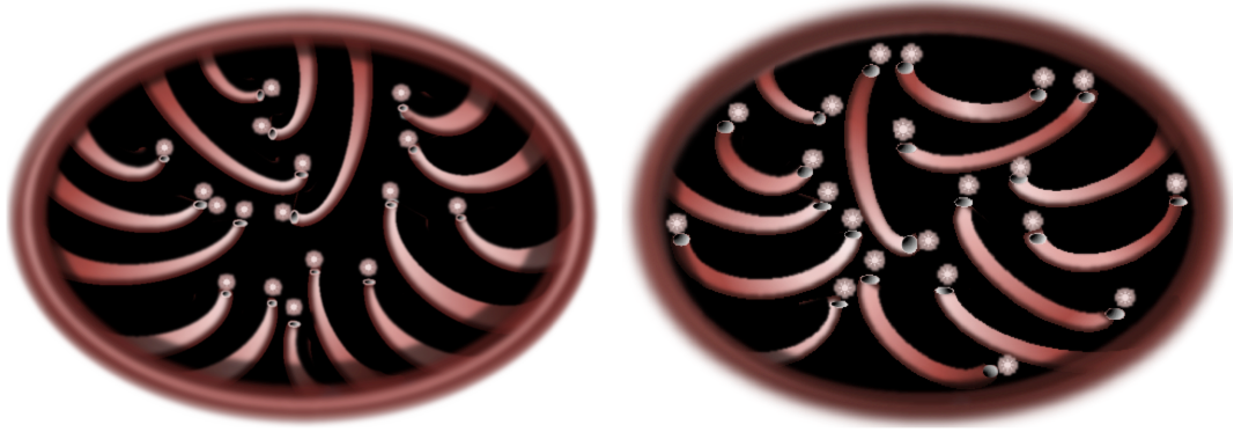
\includegraphics[scale=0.60]{SelfEntangledUniverse5.pdf}
\vspace{-0.2  cm}
\caption{\small \it Two possible quantum entanglement patterns of de Sitter space with a one-sided horizon. The entanglement between EPR pairs is represented pictorially by tiny ER-bridges. The entanglement is long range and connects bulk excitations that carry the positive dark energy either with the states on the horizon (left) or primarily with each other (right). Both situations leads to a thermal volume law contribution to the entanglement entropy.} % with each other and the horizon. This leads to a volume law contribution to the entanglement entropy. }%\break We propose that these thermal bulk excitations are associated with the positive dark energy.}
\end{center}
\vspace{-0.6 cm}
\end{figure}

 We propose that microscopically de Sitter space corresponds to an ensemble of  metastable quantum states that together carry the Bekenstein-Hawking entropy associated with the cosmological horizon. %\\[-2mm] 
%\begin{equation}
%S(L) = {A(L)\over 4G
%\hbar} \qquad \qquad \mbox{with} \qquad\qquad A(L)=\Omega_{d-2} L^{d-2}	
%\end{equation}
The metastability has purely an entropic origin: the high degeneracy together with the ultra-slow 
dynamics prevent the microscopic system to relax to the true ground state. At long timescales the microscopic de Sitter states satisfy the eigenstate thermalization hypothesis  (ETH) \cite{ETH1,ETH2}, which implies that they contain a thermal volume law contribution to the entanglement entropy.   
 
To derive the Einstein equations one requires a strict area law for the
entanglement entropy.  In condensed matter systems a strict area law arises almost exclusively 
in ground states of gapped systems with strong short range correlations. A small but non-zero volume law entropy, for instance due to thermalization, would compete with and at large 
distances overwhelm the area law. We propose that precisely this phenomenon occurs in de Sitter space and is responsible for the presence of a cosmological horizon. Our aim is to study the emergent laws of gravity in de Sitter space while taking into account its thermal volume law entropy. 
 
 

\subsection{Hints from observations: the missing mass problem}


In this paper we provide evidence for the fact that the observed dark energy %\cite{DarkEnergy} 
and the phenomena currently attributed to dark matter have a common origin and are 
connected to the emergent nature of spacetime and gravity. 
The observed 
flattening of rotation curves, as well as many other observations of dark matter phenomena, 
indicate that they are controlled 
by the Hubble acceleration scale $a_0$, as first pointed out by Milgrom \cite{Milgrom:1983}.  It is an 
empirical fact \cite{BekensteinMilgrom, Milgrom, Sanders} that the `missing mass problem', usually interpreted as observational evidence for dark matter,  only occurs when the 
gravitational acceleration %the surface mass density 
falls below a certain critical value that is of the order of $a_0$.   This criterion can be alternatively formulated in terms of the surface mass density. 

Consider a spherical region with boundary area $A(r)= 4\pi r^2$ that contains matter with total mass $M$ 
near its center. 
We define the surface mass density\footnote{Astronomers use the  
`projected' surface mass density obtained by integrating the mass density along 
the line of sight. Our somewhat unconventional definition is more convenient for our purposes.}
$\Sigma(r)$ as the ratio of the mass $M$ and the area $A(r)$. 
Empirically the directly observed gravitational phenomena attributed to dark matter, such as the flattening of rotation curves in spiral galaxies and the evidence from weak lensing data, occur when 
the surface mass density falls below a universal~value determined by the acceleration scale $a_0$
\be
\label{Sigmacrit}
\Sigma (r)=
{M\over A(r)}< {a_0\over 8\pi G}.   
\ee  
 The appearance of the cosmological acceleration scale $a_0$ in galactic dynamics is 
 striking and gives a strong hint towards an explanation in terms of emergent gravity, as envisaged in \cite{Milgromvac}. 
 To make this point more clear let us rewrite the above inequality as
\be
\label{SM0}
S_M= {2\pi M\over \hbar a_0} < {A(r)\over 4G\hbar}.
\ee
 The quantity on the l.h.s. represents the change in the de Sitter entropy 
caused by adding the mass $M$, while the r.h.s. is the entropy of a black hole 
that would fit inside the region bounded by the area $A$.  

Our goal is to  give a theoretical explanation for why the  emergent laws of gravity differ from those of general relativity precisely when the inequality (\ref{SM0}) is obeyed.  We will find that this criterion  is directly related to the presence of the volume law contribution to the entanglement entropy.   At scales much smaller than the Hubble radius gravity is in most situations well described by general relativity, because the entanglement entropy is still dominated by the area law of the vacuum.  But at large distances and long time scales the enormous de Sitter entropy in combination with the extremely slow thermal dynamics lead to modifications to these familiar laws. We will determine these modifications and show that precisely when the surface mass density falls below the value (\ref{Sigmacrit}) the reaction force due to the thermal contribution takes over from the `normal' gravity force caused by the area law. 


\subsection{Outline: from emergent gravity to apparent dark matter}


The central idea of this paper is that the volume law contribution to the entanglement entropy, associated with the positive dark energy, turns the otherwise ``stiff" geometry of spacetime  into an elastic medium. We find that the elastic response of this  `dark energy' medium takes the form of an extra `dark' gravitational force that appears to be due to `dark matter'. For spherical situations and under the right circumstances  it is shown that the surface mass densities of the baryonic and apparent dark matter  obey the following scaling relation in $d$ spacetime dimensions 
\be
\label{TF}
%{\Sigma_D^2} ={\Sigma_B\over d-1} {a_0\over 8\pi G} \qquad\qquad\mbox{with}\qquad\qquad \Sigma_D \equiv {M_D\over A},\quad \Sigma_B \equiv {M_B\over A}
{2\pi \over \hbar a_0} {M_D^2} = {A(r)\over 4G\hbar} {M_B\over d-1} \qquad\qquad\mbox{or}\qquad\qquad \Sigma_D^2(r) ={a_0\over 8\pi G} { \Sigma_B(r)\over d-1}. 
\ee  
   %  The fact 
%that the short time scale dynamics is controlled by area law entanglement implies that at these scales 
%the degrees of freedom have not thermalised. 
 %However, modifications to general relativity arise when the force induced by the thermal entropy density becomes comparable with the gravitational force obtained from the area law.  Somewhat surprisingly, this happens already in a regime where the thermal entropy itself is still much smaller than the area law entanglement entropy. 
The first equation connects to the criterion (\ref{SM0}) and makes the thermal and entropic 
origin manifest. The second relation can alternatively be written in terms of the 
%Reinstating the speed of light $c$ does not change these equations: they are dimensionally correct as they stand. 
%We will present a derivation that makes use of the volume contribution to the entanglement entropy associated to the dark energy excitations. The basic idea is that the reduction $S_M$ in the de Sitter entropy due the baryonic matter is taken out of this volume contribution.  This will lead to an `elastic' response whose magnitude we determine following general arguments. 
%The origin of the factor $d-1$ can be traced back to equation (\ref{entropydensity}) for the entropy 
%density. 
 gravitational acceleration $g_D$ and $g_B$ due to the apparent dark matter and baryons, which are related to $\Sigma_D$ and $\Sigma_B$ by
\begin{equation}
\Sigma_D = {d-2\over d-3}\, {g_D\over 8\pi G} \qquad\qquad \mbox{and}\qquad\qquad \Sigma_B = {d-2\over d-3}\, {g_B\over 8\pi G}.	
\end{equation}
Hence these accelerations obey the scaling relation
\begin{equation}
g_{D} = \sqrt{g_{B} a_M} \qquad \qquad \mbox{with}  \qquad \qquad  a_M = {(d-3) \over (d-2)(d-1)} a_0.	
\end{equation}
In $d=4$ these equations are equivalent to the baryonic Tully-Fisher relation \cite{TF-relation} that relates the velocity of the flattening galaxy rotation curves and the baryonic mass $M_B$.  In this case one finds $a_M = a_0/6$, which is indeed the acceleration scale that appears in Milgrom's phenomenological fitting formula \cite{Milgrom,Sanders}.  We like to emphasise that these scaling relations are not  new laws of gravity or inertia, but appear as estimates of the strength of the extra dark gravitational force. From our derivation it will become clear in which circumstances these relations hold, and when they are expected to fail. This point will be further clarified in the concluding section.

This paper is organized as follows. In section 2 we present our main hypothesis regarding the entropy content of de Sitter space. In section 3 we discuss several conceptual issues related to the glassy dynamics and memory effects that occur in emergent de Sitter gravity.  We determine the effect of matter on the entropy content in section 4, and explain the origin of the criterion (\ref{SM0}). We also give a heuristic derivation of the scaling relation (\ref{TF}). In section 5 we relate the definition of mass in de Sitter to the reduction of the total entropy using the Wald formalism. This serves as a preparation for section 6, where we give a detailed correspondence between the gravitational and elastic equations. 
Section 7 contains the main result of our paper: here we derive the apparent dark matter density in terms of the baryonic mass distribution and compare our findings with known observational facts.  Finally, the discussion and conclusions are presented in section 8.  



 
 %\newpage
 %....LONG RANGE ENTANGLEMENT LEADS TO THERMAL VOLUME LAW....
 
 


\newpage

\section{Dark Energy and the Entropy in de Sitter Space}

\label{sec:darkenergyandentropy}


The main hypothesis from which we will derive the emergent gravitational laws in de Sitter space, and the effects that lead to phenomena attributed to dark matter, is contained in the following two statements.  
\begin{itemize}
\item[{\it (i)}] {\it There exists a microscopic {{bulk}} perspective in which the area law for the entanglement entropy is due to the {{short distance entanglement}}  of neighboring degrees of freedom that build the emergent bulk spacetime.}
\item[({\it ii})] {\it The de Sitter entropy is evenly divided over the same  microscopic  degrees of freedom that build the emergent spacetime through their entanglement, and is caused by the {{long range entanglement}} of part of these degrees of freedom. }
\end{itemize}  


\noindent We begin in subsection \ref{subsec:datahiding} by explaining these two postulates from a quantum information theoretic perspective, and by analogy with condensed matter systems. In subsection \ref{subsec:entropycontentds} we will provide a quantitative description of the entropy content of de Sitter space. We will associate the entropy with the excitations that carry  the positive dark energy. This interpretation will be motivated in subsection \ref{subsec:towardsstring} by using insights from string theory and AdS/CFT. The details of the microscopic description will not be important for the rest of this paper. We will therefore be somewhat brief, and postpone a detailed discussion of the microscopic perspective to a future publication. 



\subsection{De Sitter space as a data hiding quantum network}

\label{subsec:datahiding}

According to our first postulate each region of space is associated with a tensor factor of the microscopic Hilbert space, so that the entanglement entropy obtained by tracing over its complement satisfies an area law given by the Bekenstein-Hawking formula. So the microscopic building blocks of spacetime are (primarily) short range entangled. This postulate is directly motivated by the Ryu-Takanayagi formula and the tensor network constructions of emergent spacetime \cite{MERA, HarlowPreskill,Haydenetal}, and is in direct analogy with condensed matter systems that exhibit area law entanglement.
 
A strict area law is known to hold in condensed matter systems 
with gapped ground states. Indeed, we conjecture that from a microscopic bulk perspective  AdS spacetimes correspond to the gapped ground states 
of the underlying quantum system.   The building blocks of de Sitter spacetime are, according to our second postulate, not exclusively short range entangled, but also exhibit long range entanglement at the Hubble scale. Again by analogy with condensed matter physics this indicates that these de Sitter states  correspond to excited energy eigenstates. Hence, the entanglement entropy contains in addition to the area law also a volume law contribution. In terms of a tensor network picture this means these states contain an amount of quantum information which is evenly divided over all tensors in the network. 

%Such states can be represented in the microscopic Hilbert space of all the tensors in such a way that the information content of the de Sitter space is evenly divided over the tensor factors. 

This can be formulated more precisely using the language of 
quantum error correction.  Quantum error correction is based on the principle that the quantum information contained in  $k$ `logical' qubits can be encoded in $n\!>\!k$ entangled `physical' qubits, in such a way that the logical qubits can be recovered even if a subset of the physical qubits is erased.   A particularly intuitive class of error correcting codes makes use of so-called `stabilizer conditions' \cite{Gottesman}, each of which reduces the Hilbert space of physical qubits by a factor of 2. By imposing $n-k$ stabilizer conditions %\footnote{these stabilizer conditions must actually form a group. We will not make use this fact, since our discussion is meant to be general and our conclusions do not rely on these specific properties of the code.} 
 the product Hilbert space of $n$-qubits is reduced to the so-called `code subspace' in which the $k$ logical qubits are stored. %The latter are referred to as the logical qubits, while the $n$ qubits are called the physical qubits.  The subspace that is obtained after imposing the stabilizer conditions is the code subspace. The $k$ logical qubits are thus encoded in the Hilbert space of the $n$ physical qubits. 
 The encoded information is robust against erasure of one or more physical qubits, if $n$ is much larger than $k$ and the transition between two different states in the code subspace requires the rearrangement of many physical qubits. 
 %The minimal number of physical qubits that needs to rearranged is called the depth $d$.  
 %Quantum error correcting codes are thus characterized by the three integers $(n,k,d)$.

These same principles apply to the entanglement properties of emergent spacetime. For AdS this idea led to the construction of holographic error correcting tensor networks \cite{HarlowPreskill,Haydenetal}. 
 These networks are designed so that they describe an encoding map from the `logical' bulk states onto the Hilbert space of `physical' boundary states \cite{Harlow}.  The tensors in the bulk of the network are usually not considered to be part of the space of physical qubits, since they do not participate in storing the quantum information associated with the logical qubits. 
  
With our first postulate we take an alternative point of view by regarding all these 
bulk tensors as physical qubits, and interpreting the short distance entanglement imposed 
by the network as being due to   stabilizer conditions.  Schematically, the Hilbert states of physical qubits are of the form\\[-2mm]
\be
   %|{\bf \Psi}\rangle = 
   \prod_x|V_x\rangle \in {\cal H}%_{enlarged} 
   \qquad\quad \mbox{with} \qquad \quad
   |V_x\rangle =\sum_{\alpha,\beta,\gamma,\ldots}\!\! V_x^{\alpha\beta\gamma\ldots}\, |\alpha\rangle|\beta\rangle|\gamma\rangle \cdots\\[-2mm]
\ee 
where $x$ runs over all vertices of the network, and $\alpha,\beta,\gamma,\ldots $  represent indices with a certain finite range $D$. In a holographic tensor network the stabilizer conditions are so restrictive that the bulk qubits are put into a unique `stabilizer state' $|\phi_0\rangle$, obtained by maximally entangling all bulk indices with neighbouring tensors.     
Again schematically, \\[-2mm]
\be
%|\Psi \rangle = |\psi_0\rangle \langle \psi_0|\,  \prod_x|V_x\rangle,
|\phi_0\rangle = \prod_{\langle xy\rangle} |xy\rangle \qquad\quad\mbox{where}\qquad\quad%\\
%\ee
%represents the unique stabilizer state given by the product over all neighboring pairs $\langle xy\rangle$ 
%of the maximally entangled states for adjacent tensor indices 
%\be
| xy\rangle = {1\over \sqrt{D} }\sum_{\alpha=1}^{D}|\alpha\rangle_x|\alpha\rangle_y.
\ee
%Therefore, we can write\\[-2mm]
%\be
%|\Psi\rangle=  \sum_{i,\alpha} A^{(0)}_{i\alpha}   |\psi_i\rangle_{{}_{bulk}}|\chi_\alpha\rangle_{{}_{bndr}} \, |\phi_0\rangle\,\\[-1mm]
%\ee
 The Hilbert space of logical qubits is generated by local bulk operators that act on 
 individual tensors.  The network defines a unitary encoding map from the logical bulk 
 qubits to the physical boundary qubits, by `pushing' the bulk operators through the network 
 and representing them as boundary operators. For this one makes use of the fact that the 
 bulk states are maximally entangled with the boundary states \cite{HarlowPreskill, 
 Haydenetal}.   This can only be achieved if the entanglement entropy in the 
 bulk obeys an area law. In other words, area law entanglement is a necessary condition for a holographic map from the bulk to the boundary. The negative curvature is also crucial 
 for a holographic description, since it ensures that after tracing out the auxiliary 
 tensors in the network, bulk excitations remain maximally entangled with the boundary. 


 
Thermal excitations compete with the boundary state for the entanglement of other bulk excitations. An individual excitation can lose its entanglement connection with the boundary by becoming maximally entangled with other bulk excitations. Simply stated: if the excited bulk states contain more information than the number of boundary states, the bulk states take over the entanglement and the holographic correspondence breaks down. This statement holds in every part of the network, and is equivalent to the  holographic bound: it puts a limit on how much information can be contained in bulk excitations before the network loses its holographic properties.

Our second postulate  states that  the quantum information measured by the area of de Sitter horizon spreads over all physical qubits in the bulk and hence becomes delocalized into the long range correlations of the microscopic quantum state of the tensor network.  By relaxing the stabilizer conditions, the quantum state of all bulk tensors %, instead of being projected onto the single stabilizer state $|\phi_0\rangle$, 
 is allowed to occupy a set of states $|\phi_I\rangle$ 
with a non-zero entropy density. Concretely this means that the tensors not only carry short range entanglement, but contain some indices that participate in the long range entanglement as well. The code subspace is thus contained in the microscopic bulk Hilbert space instead of the boundary Hilbert space. Since the quantum information is shared by all tensors, it is protected against disturbances created by local bulk operators, and therefore remains hidden for bulk observers. These delocalized states are counted by the de Sitter entropy, and contain the extremely low energy excitations that are responsible for the positive dark energy.  
 %The entanglement properties of these states differ in an essential way from the states created by local bulk operators: locally these encoded de Sitter states are indistinguishable from the vacuum because the intrinsic non-locality of the stored information does not correspond to anything that is naturally contained in the Hilbert space of local bulk excitations.  %This point will become more clear when we discuss the string theoretic perspective. 
 
%By relaxing the stabilizer conditions on the state of the bulk tensors, they are not put into a single stabilizer state but are allowed to occupy a set of delocalized states 
% with a non-zero entropy density.    
    
  When the volume becomes larger, due to the positive curvature of de Sitter space, the total quantum information stored by the collective state of the bulk tensors eventually exceeds the holographic bound.  At that moment the bulk states  take 
  over the entanglement, and local bulk operators are no longer mapped holographically to boundary operators. The breakdown of the area law entanglement at the horizon thus implies  that de Sitter space does not have a holographic description at the horizon.  The would-be horizon states themselves become maximally entangled with the thermal excitations that carry the volume law entropy. As a result they become delocalized and are spread over the entangled degrees of freedom that build the bulk spacetime.  Note that these arguments are closely related to the discussions that led to the firewall paradox \cite{AMPS}, EPR=ER proposal \cite{ER=EPR} and the ideas of fast scrambling \cite{FastScrambler} and computational complexity \cite{Complexity}.  The size of the Hilbert space of bulk states is exactly given by the horizon area, since this  is where the volume law   exceeds the area law   entanglement entropy. In other words, de 
  Sitter space  contains exactly the limit of its storage capacity determined by the horizon 
  area.  In the condensed matter analogy, the breakdown of holography corresponds to a localization/de-localization  transition \cite{Grover} from the localized boundary states into delocalized states that occupy the bulk. 
  
  %After the transition the information is equally 
  %shared by all the tensors, and hence the entropy in each region is given by (\ref{Svol}). 
  

  



%This brings us to our main hypothesis. We postulate that the de Sitter entropy is distributed over the bulk spacetime with a density given by (\ref{entropydensity}). Specifically  we will assume the entropy content inside a sphere of radius $r$ centered around the origin is given by

%XXXX




\subsection{The entropy content of de Sitter space}

\label{subsec:entropycontentds}

Next we give a quantitative description of the entropy content of de Sitter space for 
the static coordinate patch described by the metric\\[-2mm] 
\begin{equation}
\label{deSitter}
ds^2 = -f(r) dt^2 + {dr^2\over f(r)} +r^2d\Omega^2\\[-2mm] 
\end{equation}
where the function $f(r)$ is given by\\[-4mm]
\begin{equation}
f(r) =1-{r^2\over L^2} \, .
\end{equation}
We take the perspective of an observer near the origin $r=0$, so that the edge of
his causal domain coincides with the horizon at $r=L$. The horizon entropy equals 
\be
\label{dSentropy}
 S_{DE}(L) = {A(L)\over 4G\hbar} %= {r\over L} {A(r)\over 4G\hbar} 
 \qquad\qquad \mbox{with} \qquad\qquad A(L) = \Omega_{d-2} L^{d-2} ,
\ee
where $\Omega_{d-2}$ is the volume of a ($d-2$)-dimensional unit sphere.
Our hypothesis is that this entropy is evenly distributed over microscopic 
degrees of freedom that make up the bulk spacetime. To determine the entropy density we view  
the spatial section at $t=0$ as a ball with radius $L$ bounded by the horizon. 
The total de Sitter entropy is divided over this volume so that a ball of radius $r$ 
centered around the origin contains an entropy $S_{DE}(r)$ proportional to its volume\\[-2mm]
%$V(r) = {1\over d-1}\Omega_{d-2} r^{d-1}$,  
\be
\label{entropyhypothesis}
 S_{DE}(r) = {1\over V_0}  V(r) %= {r\over L} {A(r)\over 4G\hbar} 
 \qquad\qquad \mbox{with} \qquad\qquad V(r) = {\Omega_{d-2}  r^{d-1} \!\!\!\over \! \!\! d-1} .
%\qquad \mbox{and} 
%\qquad V_0 ={4G\hbar L\over d-1}.
\ee
%Here and throughout most of this paper we work in general 
%spacetime dimension $d$. 
The subscript $DE$ indicates that the entropy is carried by excitations of the 
microscopic degrees of freedom that lift the negative ground state energy to the positive value associated with the dark energy. This point will be further explained below. 

The value of the volume $V_0$ per unit of entropy follows from the requirement that 
the total entropy $S_{DE}(L)$, where we put   $r=L$, equals the Bekenstein-Hawking entropy associated with the cosmological horizon. 
By comparing (\ref{entropyhypothesis}) for $r=L$ with (\ref{dSentropy}) one obtains that  
  $V_0$  takes the value\\[-2mm]
\be
V_0 ={4G\hbar L\over d-1} 
\label{entropyvolume}  
\ee
where the factor $(d-1)/L$ originates from the relative normalization of the horizon area $A(L)$ and the volume $V(L)$. This entropy density is thus determined by the Planck area and the Hubble scale. In fact, this value of the entropy density has been proposed as a holographic upper bound in a cosmological setting.% \cite{FSB}.  
%Just to get a feeling for the magnitude of $V_0$: it is about the size of a proton. 


An alternative way to write the entropy $S_{DE}(r)$ is in terms of the area $A(r)$ as\\[-2mm]
\begin{equation}
\label{Svol}
S_{DE}(r) % ]{1\over V_0} V(r) 
= 
{r\over L} {A(r)\over 4G\hbar}  \qquad \qquad \mbox{with} \qquad\qquad  A(r) = \Omega_{d-2} r^{d-2}  . 	
\end{equation}
From this expression it is immediately clear that when we put $r=L$ we recover the Bekenstein-Hawking entropy (\ref{dSentropy}). 
%It also suggests that at radius $r<L$  only a fraction $r/L$ of the maximal entropy that is allowed by the holographic principle is occupied. From the perspective described in the previous section this is rather natural, since the quantum information is evenly shared over all bulk degrees of freedom. 



 



\subsection{Towards a string theoretic microscopic description} 

\label{subsec:towardsstring}

We now like to give a more string theoretic interpretation of these formulas and also further motivate why we associate this entropy with the positive dark energy.  For this purpose it will be useful to make a comparison between de Sitter space with radius $L$ and a subregion of AdS that precisely fits in one AdS radius $L$.  
We can write the AdS metric in the same form as (\ref{deSitter})
%\begin{equation}
%\label{deSitter}
%ds^2 = -f(r) dt^2 + {dr^2\over f(r)} +r^2d\Omega^2 
%\end{equation}
except with $f(r) =1+ r^2/L^2.$
For AdS it is known \cite{AdS-CFT,  SusskindWitten} that the number of quantum 
mechanical degrees of freedom associated with a single region of size $L$ is determined by the central charge of the CFT  %in terms of the radius $L$ and Newton's constant via 
\be
{\cal C}(L) = {A(L)\over 16\pi G\hbar} = \ \mbox{\# of degrees of freedom}.
\ee
This is the analogue of the famous Brown-Henneaux formula 
\cite{Brown-Henneaux}: for AdS$_3$/CFT$_2$ it equals $c/24$, while in other dimensions it is 
the central charge defined via the two-point functions of the stress tensor. In string theory these degrees of freedom describe a matrix or quiver quantum mechanics 
obtained by dimensional reduction of the CFT. 


We postulated that $A(L)/4G\hbar$ corresponds to the entanglement entropy of the vacuum 
state when we divide the state into two subsystems inside and outside of the single AdS regions. This 
quantity can also be computed in the boundary CFT, where it corresponds to 
the so-called `differential entropy' \cite{holeography}. To obtain this result as a 
genuine entanglement entropy one has to extend the microscopic Hilbert  space by 
associating to each AdS region a tensor factor. This tensor factor represents the Hilbert 
space of the (virtual) excitations of the  ${\cal C}(L)$ quantum mechanical degrees of 
freedom. 

Let us compute the `vacuum' energy in (A)dS contained inside a sphere of radius $r$
\be
E_{(A)dS}(r) = %= - E^{AdS}_{vac}(r) = %\mp {1\over 2} {r^2\over L^2} {d{\cal C}(r)\over dr} 
\pm {(d-1)(d-2) \over 16\pi GL^2} V(r) = \pm \left({r\over L}\right)^{d-1} \hbar {d-2\over L}  {\cal C}(L) . %\qquad \quad\mbox{with} \qquad\quad  V(r) ={\ \,\Omega_{d-2} r^{d-1}\over d-1} 
\ee
 The negative vacuum energy in AdS can be understood as the Casimir energy associated with the number of microscopic degrees of freedom; indeed, this is what it 
corresponds to in the CFT. We interpret the  positive dark energy in de Sitter space as the excitation energy that lifts the vacuum energy from its ground state value. To motivate this assumption, let us give a heuristic derivation of the entropy of de Sitter space as follows. Let us take $r=L$ and write the `vacuum' energy for AdS in terms of ${\cal C}(L)$ as\\[-2mm]
\be
\label{Casimir}
%E_{vac}^{\, dS}(L) = {d-2\over L}\, {\cal C}(L),  \qquad \qquad  
E_{AdS}%_{vac}^{\,AdS}
(L) = -\, \hbar \,{d-2\over L}\, {\cal C}(L).
\ee
For dS we write the `vacuum' energy in a similar way in terms of the number of excitations ${\cal N}(L)$ of energy $\hbar (d-2)/L$ that have been added to the ground state  
 \be
\label{Estar}
E_{dS}(L) = \,\hbar\, {d-2\over L} \,\Bigl({\cal N}(L)-{\cal C}(L)\Bigr) \qquad \quad\mbox{where}\quad \qquad {\cal N}(L) = 2 \, {\cal C}(L). 
\ee
We now label the microscopic states by all possible ways in which the  ${\cal N}(L)$ 
 excitations can be distributed over the ${\cal C}(L)$ degrees of freedom. The computation 
 of the entropy then reduces to a familiar combinatoric problem, whose answer is given by 
 the Hardy-Ramanujan formula\footnote{ The result (\ref{Cardy}) looks identical to the Cardy formula, but does not require the existence of 2d-CFT. Similar expressions for the holographic entropy have been found in \cite{CV, PadmaVirasoro}.}\\[-3mm]
\be
\label{Cardy}
S_{DE}(L) =4\pi \sqrt {{\cal C}(L)\Bigr({\cal N}(L)-{\cal C}(L)\Bigr)}. %= 4\pi \, {\cal C}(L) = {A(L)\over 4G\hbar}
\ee
%where we used that the effective number of excitations ${\cal N}(L)-{\cal C}(L)$ is equal to ${\cal C}(L)$. 
One easily verifies that this agrees with (\ref{dSentropy}). From a string theoretic perspective this indicates that the ${\cal C}(L)$ microscopic degrees of freedom live entirely on the so-called Higgs branch of the underlying matrix or quiver quantum mechanics.

These  ${\cal C}(L)$ quantum mechanical degrees of freedom do not suffice to explain the area law entanglement at sub-AdS scales. For this it is necessary to extend the Hilbert space even further by introducing additional auxiliary degrees of freedom that represent additional tensor factors for much smaller regions, say of size $\ell<\!\!L$.  The total number of degrees of freedom has increased by a factor $L/\ell$ and equals
\be
%{L\over r} \, {\cal C}(L)  = 
\left({L^{d-1}\over \ell^{d-1}}\right) {A(\ell)\over 16\pi G\hbar} =  \mbox{\# of auxiliary degrees of freedom}. %=  \left(L\over \ell\right){\cal C}(L)
\ee
%Both from the tensor network as well as the string theoretic perspective in terms of quiver quantum mechanics, one can naturally add such auxiliary degrees of freedom.  
In the tensor network $\ell$ represents the spacing between the vertices of a fine grained 
network, while in the quiver matrix quantum mechanics one can view $\ell$ as the `fractional string scale' of a fine grained matrix quiver quantum mechanics model. The precise value of the UV scale $\ell$ turns out to be unimportant for the 
macroscopic description of the emergent spacetime.  For instance, in the tensor network one can combine several tensors to form a larger tensor without changing the large scale entanglement properties, while in the string theoretic description one can view $\ell$ as the `fractional string scale' of a  fine grained matrix quiver quantum mechanics model.  

By increasing the number of degrees of freedom by a factor $L/\ell$ one also has increased the energy gap required to excite a single auxiliary degree of freedom with the same factor. Hence, instead of $(d-2)/L$ the energy gap is now equal to
$(d-2)/\ell$.   This means that  the number of excitations has decreased by a factor $\ell/L$, since the total energy has remained the same.  One can show that this combined operation leaves the total entropy $S_{DE}(L)$  invariant. 
In string theory this procedure is known as the  `fractional string' picture, which is the inverse of the `long string phenomenon'. 
 Each region of size $\ell$ in de Sitter space contains a fraction $(\ell/L)^{d-1}$ of the total 
 number of auxiliary degrees of freedom, as well as a fraction $(\ell/L)^{d-1}$ of the total number of excitations.  This means it also carries a fraction $(\ell/L)^{d-1}$  of the total entropy    
 \be
 \label{fracS}
 S_{DE}(\ell)  = {\ell\over L} {A(\ell)\over 4G\hbar}.
 \ee
%In other words, the de Sitter entropy is shared by degrees of freedom that build the bulk spacetime.
Since the scale $\ell$ can be chosen freely, we learn that the entropy content of a spherical region with arbitrary radius $r$ is found by putting $\ell =r$ in (\ref{fracS}).  A more detailed discussion of this string theoretic perspective will be presented elsewhere. 









%In this subsection we further elaborate the string theoretic description, in particular focus on the different roles played by the `vacuum' energy in AdS and dS. 


%In this section we present a microscopic bulk perspective on emergent spacetime and describe our main hypothesis regarding the entropy content of de Sitter space.  Subsequently we give additional motivation and justification for our hypothesis first from a quantum information theoretic point of view, and subsequently from a string theoretic perspective. Both descriptions will be brief, since our further explorations will not depend on the details of the underlying microscopic theory. 

  
%In general relativity the cosmological constant can be set freely, but in a theory of emergent gravity one likes to say more about its origin. 
%We first discuss the negative vacuum energy of AdS.  The total vacuum energy inside a region with 
%radius $r$ equals 
%\be
%E_{vac}^{\, dS}(r) ={1\over 2}E^*(r), \qquad \qquad  
%E_{vac}^{\,AdS}
%(r)= -{(d-1)(d-2) \over 16\pi GL^2} V(r),  \qquad \quad\mbox{where}\qquad\quad V(r)= {\Omega_{d-2} r^{d-1}\over d-1}\ee
%is the volume of that region. 

%We interpret this negative ground state energy as a Casimir energy: indeed, this is what it 
%corresponds to in the CFT. When we  put $r=L$ we can express the Casimir energy in terms of 
%the central charge ${\cal C}(L)$ 
%as
%\be
%\label{Casimir}
%E_{vac}^{\, dS}(L) = {d-2\over L}\, {\cal C}(L),  \qquad \qquad  
%E_{AdS}%_{vac}^{\,AdS}
%(L) = -\, \hbar \,{d-2\over L}\, {\cal C}(L).
%\ee
%of the AdS vacuum energy as well as the positive dark energy in dS.  
%Having explained the negative vacuum energy in AdS is being due to the Casimir effect, we now propose that the positive dark energy in de Sitter space is caused by excitations that lift the microscopic theory from its ground state. This motivates us to
% write the function $f(r)$ in the metric (\ref{deSitter}) as
%\be
%f(r) = 1+ {r^2\over L^2} 
%+ 2\widetilde{\Phi}(r)\qquad\quad\mbox{with}\qquad\quad \widetilde{\Phi}(r) = - {8\pi G %\bigl(%M+E^*(r)\bigr)
%\bigl(
%E_*(r)%\!+\! E_{vac}^{AdS}(r)\bigr)
%\over (d-2)\Omega_{d-2} \,r^{d-3}}
%\ee

%This interpretation of the positive dark energy is motivated by the following natural 
%explanation of the de Sitter entropy. First let us write the excitation energy in a similar way as (\ref{Casimir}) in terms of the number of 
%excited degrees of freedom
%\be
%\label{Estar}
%E_{dS}(L) = \,\hbar\, {d-2\over L} \,\Bigl({\cal N}(L)-{\cal C}(L)\Bigr) \qquad \quad\mbox{where}\quad \qquad {\cal N}(L) = 2 \, {\cal C}(L). 
%\ee
 




%\subsection{Delocalization of de Sitter entropy.}







%(\ref{deSitter})
%\begin{equation}
%\label{deSitter}
%ds^2 = -\left(1\pm {r^2\over L^2}\right) dt^2 + {dr^2\over 1\pm r^2/L^2} +r^2d\Omega^2 
%\end{equation}
%where $f(r) = 1\pm r^2/L^2$ 
%and 
%We are interested in comparing the entanglement structure of AdS for the region with $r\leq L$ and   %In the dS case the entropy associated with the cosmological horizon is given by
%\be
%\label{SL}
%S(L) = {A(L)\over 4G\hbar} \qquad\qquad\mbox{with}\qquad \qquad A(L)=\Omega_{d-2} L^{d-2}.
%\ee


 
%We are particularly interested in studying the differences between de Sitter and anti-de Sitter space, and 
%in understanding the implications of these differences for the emergent laws of gravity.  


 

%Consider the static patch of de Sitter space and think of its
%spatial section as a ball with a radius $L$ bounded by the horizon. 
%The entropy associated with the cosmological horizon equals
%We are interested in the question where the microscopic degrees of freedom that are carrying the entropy associated to the horizon 
%\be
%\label{SCL}
%S(L) =
%{A(L)\over 4G\hbar}
%\ee
%\be
%\label{SCL}
%S(L) = {A(L)\over 4G\hbar}  %\qquad\qquad\mbox{with}\qquad \qquad 
%\ee
%are located.  Although our main focus is on de Sitter space, 

%The entropy of an AdS black hole with radius $L$ is also given by (\ref{SCL}). This result  can be intuitively understood as counting all the possible excitations of the ${\cal C}(L)$ degrees of freedom. 

%In this enlarged Hilbert space, in which one assigns a tensor factor of the microscopic Hilbert space to each AdS-region in the bulk, the differential entropy of the boundary CFT describes the actual the entanglement entropy of the vacuum state of the  microscopic degrees of freedom that build the emergent spacetime geometry. 

%We now want to extend these ideas to a de Sitter space with the same radius $L$ and hence the same entropy (\ref{SCL}). It is clear that de Sitter space differs from a single AdS region and  from an AdS black hole. To explain in what way de Sitter space is different we need to compare its microscopic entanglement structure with these other spaces at scales much smaller than the curvature radius $L$.  In empty AdS,  
%But at large scales and in the weak gravity regime the thermal entropy will have an
%important effect on the emergent gravitational force. 
%   The 
%unexpected large distance and long time scale phenomena 
%associated with the `apparent dark matter' is thus caused by the competition between the area 
%law  entanglement and the thermal entropy of the microscopic quantum state of our universe.  
%, whose strength we will compute and compare to the observable data in galaxies and clusters. 

%It is well known that adding matter with mass $M$ to empty de Sitter space reduces the entropy by the 
%amount
%\be
%S_M= {2\pi M\over \hbar a_0}.
%\ee    

%First of all, the volume law entropy is 
%caused by the excitations that are responsible for lifting the energy of the microscopic 
%quantum state from its ground state and thus for giving de Sitter space its positive dark 
%energy. 
%These facts will have important consequences for the emergent gravitational force. 

%In this section we present our main postulates and describe the central assumptions that will form the starting points of our theoretical description of emergent gravity in de Sitter space.  

%\subsection{A microscopic bulk perspective on emergent spacetime}



%In these models spacetime is built by entangling tensors located at the vertices of a network.  The general arguments presented in \cite{HarlowPreskill,Haydenetal,Haydenetal2} make clear that 
%an essential requirement for the existence of a holographic bulk to boundary map is that the area law for the entanglement entropy remains to valid  all the way to the boundary.  The reason is that the holographic  description requires that bulk excitations stay maximally entangled with the boundary degrees of freedom.  In Anti-de Sitter space it is sufficient to verify the area law condition at sub-AdS scales, since after that it is guaranteed to hold on all scales due to the negative curvature. 
%These observations also make clear that the entanglement structure of de Sitter space differs in an essential way from that of AdS. 


%In this section we are interested in the entanglement structure and the entropy content of de Sitter space. It is clear that the entanglement  properties of dS differ in an essential way from those of AdS due to the positive dark energy and positive curvature.   Ideally one would like to have a microscopic description of de Sitter space from which one can derive the entanglement entropy and study its properties. For the purpose of this paper, however,  we need very little information about the microscopic theory. The only required input for our derivation of the Tully-Fisher relation is the distribution of the entropy content of de Sitter space.  Therefor, instead of proposing a specific `ad hoc' microscopic description, we will formulate a number of postulates that will be used as starting points for our further discussion and calculations. These postulates are based on combined insights from black hole physics, string theory, and (tensor network models of) AdS/CFT, some of which we will describe below. 




%A priori the degrees of freedom responsible for the area law entanglement have nothing to do with particles or fields in spacetime: these will appear as a low energy effective description of the emergent dynamics.  We assume that this emergent dynamics is driven by the entanglement of the underlying degrees of freedom, and since their degree of entanglement  is directly related to their proximity, the apparent locality of the emergent dynamics is built in from the outset. %Furthermore, with these rules the spacetime geometry gives by construction a representation of the entanglement structure of the microscopic quantum state.  
%The entanglement in the microscopic theory bulk is thus by construction dominated by short range correlations between neighboring degrees of freedom, and hence it naturally obeys an area law.   

\section{Glassy Dynamics and Memory Effects in Emergent Gravity }

In this section we address an important conceptual question.  How can a theory of emergent gravity lead to observable consequences at astronomical and cosmological scales? We also discuss important features of the microscopic de Sitter states such as their glassy behaviour and occurrence of memory effects. These phenomena play a central role in our derivation of the emergent laws of gravity at large scales. 

\subsection{The glassy dynamics of emergent gravity in de Sitter space}
 
The idea that emergent gravity has observational consequences at cosmological scales may be counter-intuitive and appears to be at odds with the common believe that effective field theory gives a reliable description of all infrared physics.  With the following discussion we like to point out a loophole in this common wisdom. In short, the standard arguments overlook the fact that it is logically possible that the laws which govern the long time and distance scale dynamics in our universe are decoupled from the emergent local laws of physics described by our current effective field theories. 

 The physics that drives the evolution of our universe at large scales is, according to our proposal, hidden in the slow dynamics of a large number of delocalized states whose degeneracy, presence and dynamics are invisible at small scales. Together these states carry the de Sitter entropy, but they store this information in a non-local way. So our universe contains a large amount of quantum information in extremely long range correlations of the underlying microscopic degrees of freedom.   The present local laws of physics are not capable of detecting or describing these delocalized states. 

The basic principle that prevents a local observer from accessing these states is similar to the way a quantum computer protects its quantum information from local disturbances. It is also analogous to the slow dynamics of a glassy system that is unobservable on human timescales. At short observation times a glassy state is indistinguishable from a crystalline state, 
and its effective description would be identical. Its long timescale dynamics, however, differs 
drastically. Glassy systems exhibit exotic long timescale behavior such as slow 
relaxation, aging and memory effects. At the glass 
transition the fast short distance degrees of freedom fall out of equilibrium, 
while the slow long distance dynamics remains ergodic. Therefore, the long time phenomena of a glassy system cannot be derived from the same effective description as the short time behavior, since the latter is identical to that of the crystalline state.  To develop an effective theory for the slow dynamics of a glassy state one has to go back to the  microscopic description 
%from which %the effective short time scale description was derived, 
and properly understand the origin of its glassy behavior. 
%For most glassy systems the latter problem is notoriously difficult, and has not been solved in general.   

We propose that microscopically the same physical picture applies to our universe. De Sitter space behaves as a glassy system with a very high information density that is 
slowly being manipulated by the microscopic dynamics.  
The short range `entanglement bonds' between the microscopic degrees of freedom, which give rise to the area law entanglement entropy,  are very hard to change 
without either invoking extremely high energies or
having to overcome huge entropic barriers. %These short distance degrees of 
%freedom are thus `frozen' and can become `localised' in a non-equilibrium state. 
The slow dynamics together with the large degeneracy causes the 
microscopic states to remain trapped in a local minimum of an extremely large free energy landscape. %: since the short time dynamics is not ergodic, these states keep a long memory of their history and store a large amount of information.  
Quantum mechanically this means these states violate ETH at short distance and time scales. We believe this can be understood as a manifestation of many-body localization: a quantum analogue of the glass transition known to imply area law entanglement \cite{Huse1, Grover}.  

\subsection{Memory effects and the `dark' elastic phase of emergent gravity}

Matter normally arises by adding excitations to the ground state. In our description of de Sitter space there is an alternative possibility, since it already contains delocalized excitations that constitute the dark energy. Matter particles correspond to localized excitations. Hence, it is natural to assume that at some moment in the cosmological evolution these localized excitations  appeared via some transition in the delocalized dark energy excitations. The string theoretic perspective described in section 2.3 suggests that the dark energy excitations are the basic constituents in our universe. Matter particles correspond to bound states of these basic excitations, that have escaped the dark energy medium.  In string theory jargon these degrees of freedom have escaped from the `Higgs branch' onto the `Coulomb branch'.  

The dark energy medium corresponds to the entropic phase in which the excitations distribute themselves freely over all available degrees of freedom: this is known as the Higgs branch.  Particles correspond to bound states that can move freely in the vacuum spacetime. These excitations live on the Coulomb branch and carry a much smaller entropy.  Hence, the transition from dark energy to matter particles is associated with a reduction of the energy and entropy content of the dark energy medium. 

After the transition the total system contains a dark energy component as well as localized particle states.  This means that the microscopic theory corresponds to a matrix or quiver quantum mechanics that is in a mixed Coulomb-Higgs phase.\footnote{The possibility of a mixed Higgs-Coulomb branch in matrix QM was first pointed out in \cite{WittenHiggs}.}  We are interested in the question how the forces that act on the particles on the Coulomb branch are influenced by the presence of the excitations on the Higgs branch.  Instead of trying to solve this problem using a microscopic description, we will use an effective macroscopic description based on general physics arguments. 

The transition by which matter   appeared has removed an amount of energy and entropy from the underlying microscopic state.  The resulting redistribution of the entropy density with respect to its equilibrium position is described by a displacement vector $u_i$.  Since we have a system with a non-zero temperature, the displacement of entropy leads to a change in the free energy density. The effective theory that describes the response due to the displacement of the free energy density already exists for a long time, and is older than general relativity itself: it is the theory of elasticity. 

 \begin{figure}[btp]
\begin{center}
\vspace{-2.2 cm}
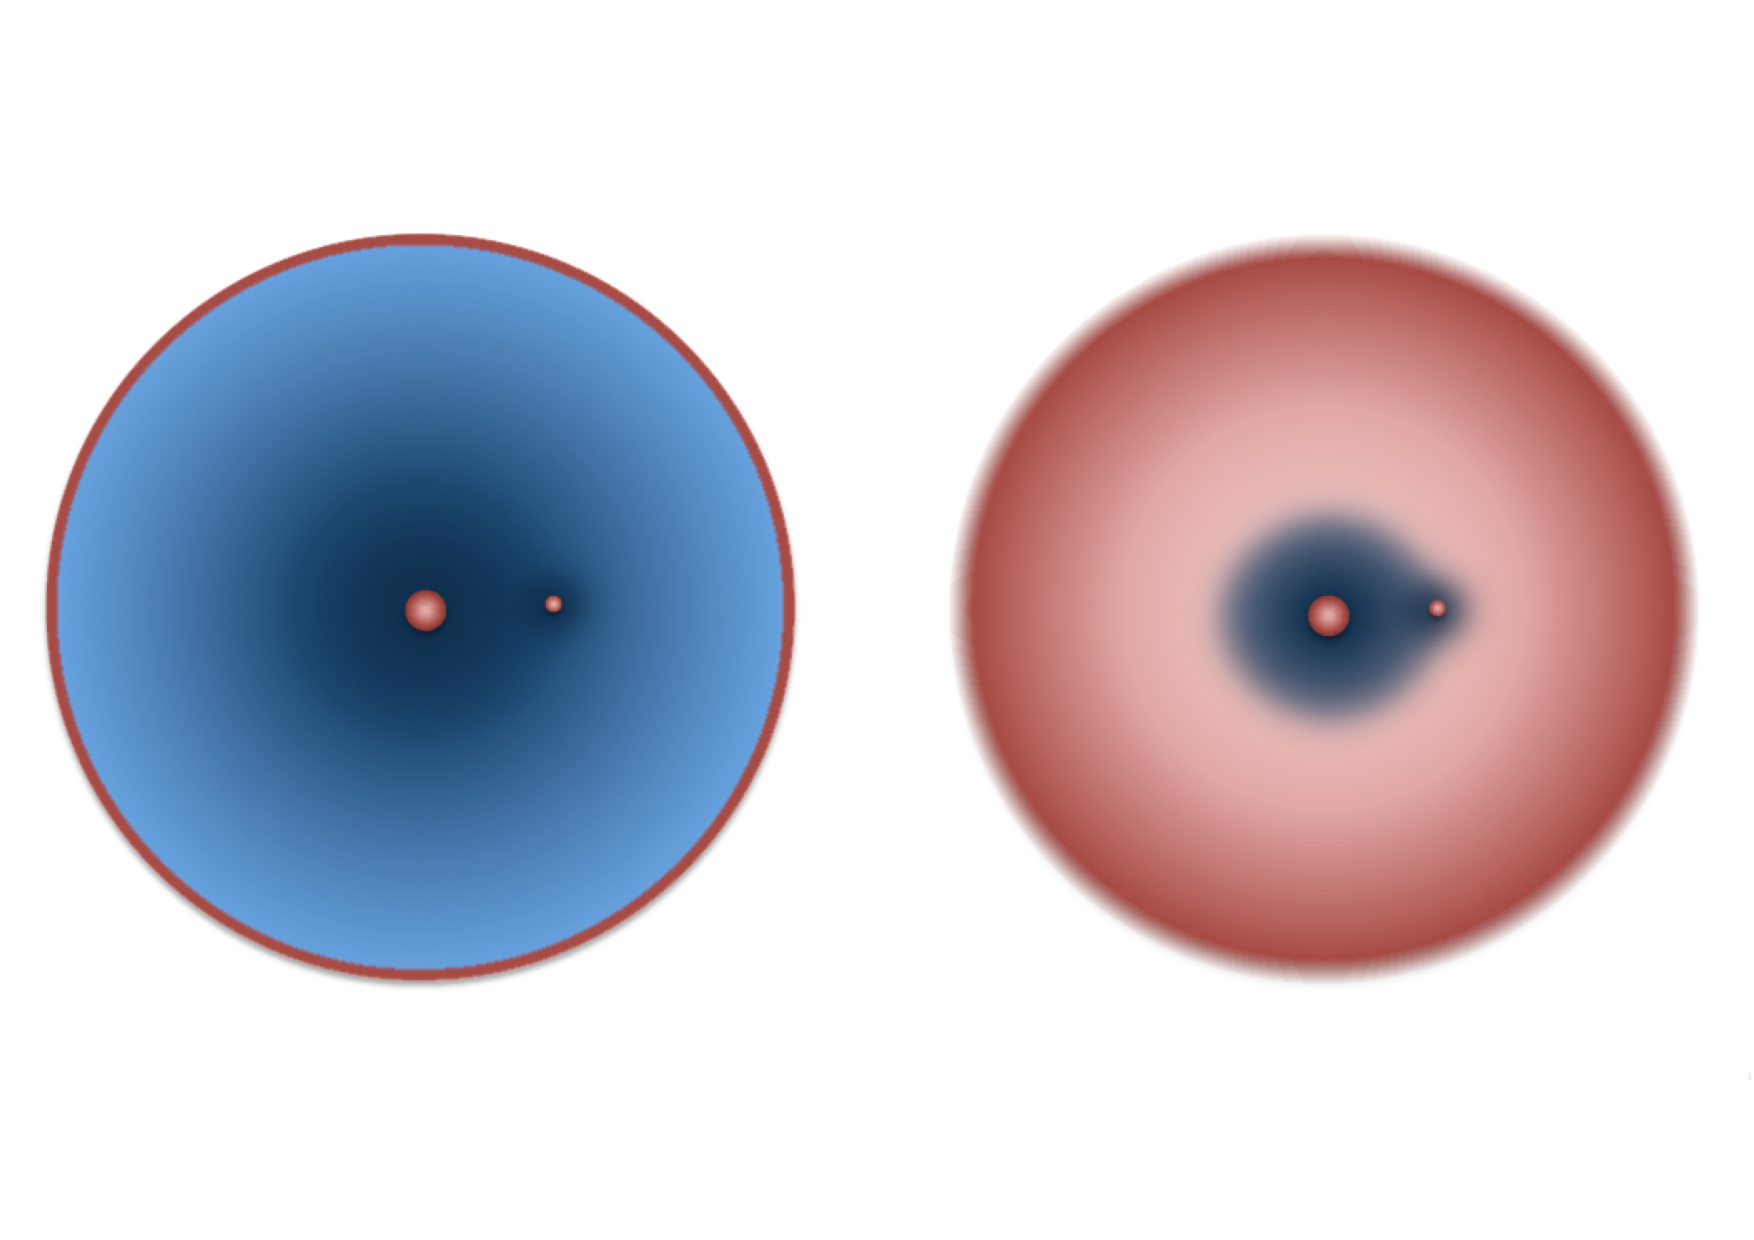
\includegraphics[scale=0.40]{ElasticPhase3.pdf}
\vspace{-2.0 cm}
\end{center}
\caption{\small \it  In AdS (left) the entanglement entropy obeys a strict area law and all information is stored on the boundary.  In dS (right) the information delocalizes into the bulk volume. Only in dS the matter creates a memory effect in the dark energy medium by removing the entropy from an inclusion region.}
\end{figure}


 As we have argued, due to the competition between the area law and volume law entanglement, the microscopic de Sitter states exhibit glassy behavior leading to slow relaxation and memory effects.  For our problem this means the displacement of the local entropy density due to matter is not immediately erased, but leaves behind a memory imprint in the underlying quantum state.  This results in a residual strain and stress in the dark energy medium, which can only relax very slowly.  


In our calculations we will make use of concepts and methods that have been developed in totally different contexts: the first is the study   by Eshelby \cite{Eshelby} of
residual strain and stress that occur in manufactured metals that undergo a martensite transition in small regions (called `inclusions'). The second is a computation by  Deutsch \cite{Deutsch} of memory effects due to the microscopic dynamics of entangled polymer melts.  In all these situations the elastic stress originates from a transition that has occurred in  part of the medium, without the system    being able to relax to a stress-free state due to the slow `arrested' dynamics of the microscopic state and its enormous degeneracy. 

The fact that matter causes a  displacement of the dark energy medium implies that the medium also causes a reaction force on the matter.  The magnitude of this elastic force is determined in terms of the residual elastic strain and stress. We propose that this  force leads to  the excess gravity that is currently attributed to dark matter. 
Indeed, we will show that the observed relationship between the surface mass densities of the apparent dark matter and the baryonic matter naturally follows by applying old and well-known elements of the (linear) theory of elasticity.  The main input that we need to determine the residual strain and stress is the amount of entropy $S_M$ that is removed by matter. 

In the following section we make use of our knowledge of emergent gravity in Anti-de Sitter space (and flat space) to determine how much entropy is associated with a mass $M$.  The basic idea is that in these situations the underlying quantum state only carries   area law entanglement.  Hence, we can determine the entropy $S_M$ associated with the mass $M$ by studying first the effect of matter on the area entanglement using general relativity. Once we know this amount, we subsequently apply this in de Sitter space to determine the reduction of the entropy density.  From there it becomes a straightforward application of linear elasticity to derive the stress and the elastic force. 









To derive the strength of this dark gravitational force  we assume that a transition occurs in the 
medium by which a certain amount $S_M$ of 
the entropy is being removed from the underlying 
microscopic state locally inside 
a certain region ${\cal V}_M$. 
%Furthermore, we assume that {\it all} of the entropy that was originally inside of this region is removed.  
Following \cite{Eshelby} we will refer to the region  ${\cal V}_M$ 
as the `inclusion'.  It is surrounded by the original medium, which will be called the 
`matrix'. 





\section{The Effect of Matter on the Entropy and Dark Energy}


In this section we determine the effect of matter on the entropy content in de Sitter space. First we will determine the change in the total de Sitter entropy when matter with a total mass $M$ is added at or near the center of the causal domain. After that we also derive an estimate of the change in the entanglement entropy by computing the deficit in (growth of the) the area as a function of distance.  We will find that this quantity is directly related to the ADM and Brown-York definitions of mass in general relativity. We subsequently determine the reduction of the entropy content of de Sitter space within a radius $r$ due to (the appearance of) matter and compute the resulting displacement field. Using an analogy with the theory of elasticity we then present a heuristic derivation of the Tully-Fisher scaling law. 

%We propose that the gravitational force currently attributed to dark matter is actually caused by the elastic response due to the displacement of the entropy content of de Sitter space induced by matter.  The de Sitter entropy is according to our basic hypothesis, associated with thermal excitations of the bulk space time that together make up the positive dark energy. This point of view will be further motivated in our discussion of the microscopic perspective. For the purpose of calculating the effects of the entropy displacement it suffices to use an effective description of the dark energy as an elastic medium with a positive free energy density. Indeed, the observed relationship between the surface mass densities of the apparent dark matter and the baryonic matter can be naturally understood from old and well known elements of the (linear) theory of elasticity. 

%According to the linear theory of elasticity the elastic strain and stress of an elastic medium 
%is proportional to the derivative of the displacement field.  The ratio $\epsilon(r)$ defined in (\ref{vareps}), turns out to be directly related to the elastic strain due to the displacement field $u(r)$. In addition,  


%In this section we summarize the most important results and main conclusions of this paper. We also present some of the central conceptual arguments, and give an outline.  

%\subsection{Area law versus volume law entanglement.}

%paper. Specifically,  we focus on the competing roles played by area law entanglement and thermal volume law entropy, and explain the origin of the glassy dynamics and memory effects that occur in quantum states in which both are present.


% Not all microscopic quantum states correspond to classical spacetime geometries. States that have a classical spacetime interpretation are. 


\begin{figure}[btp]
\begin{center}
\vspace{-1.4 cm}
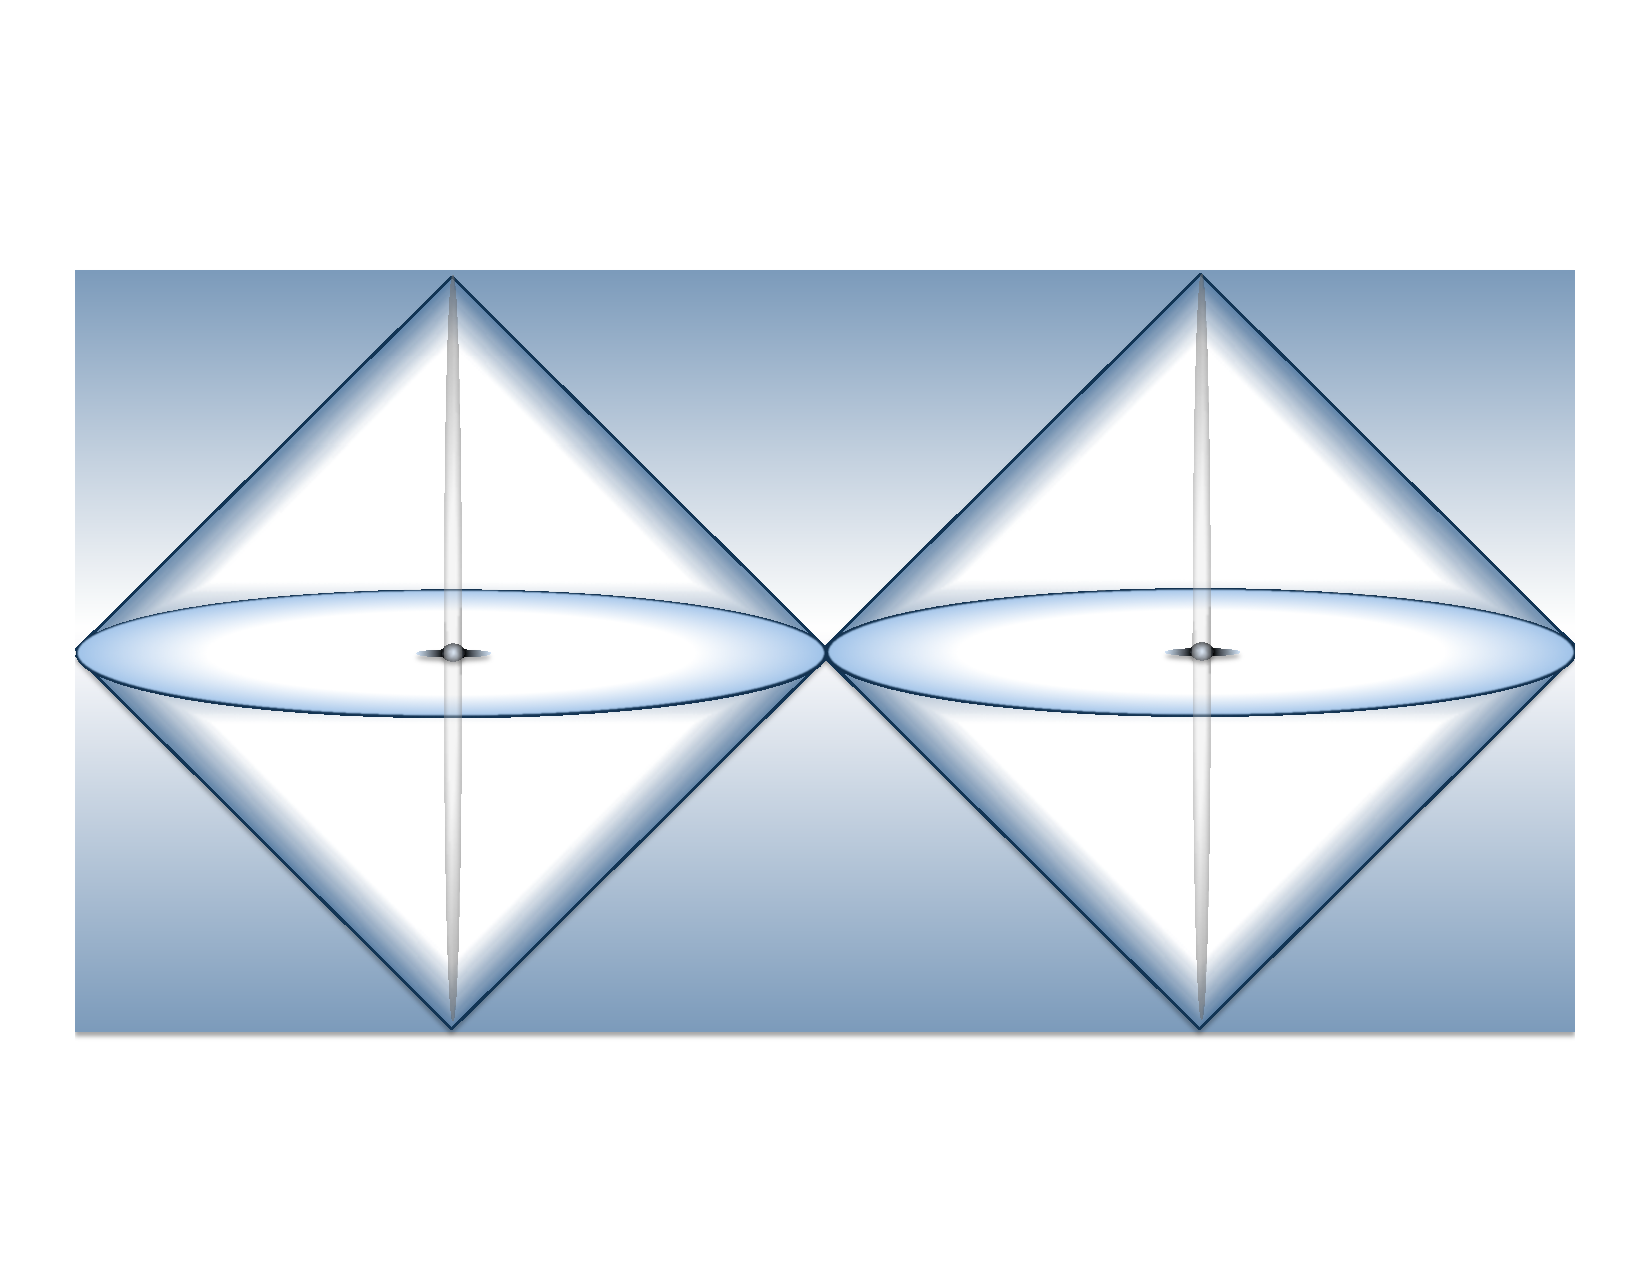
\includegraphics[scale=0.44]{Global-dS.pdf}
\vspace{-1.6 cm}
\caption{\small \it The Penrose diagram of global de Sitter space with a mass in the center of the static patch. The global solution requires that an equal mass is put at the anti-podal point.}
\label{prenroseglobal}
\end{center}
\vspace{-0.2 cm}
\end{figure}

  
 \subsection{Entropy and entanglement reduction due to matter}
 

 
We start by showing that adding matter to de Sitter space decreases its entropy content. This fact is of central importance to our arguments in this and the next sections.  % The causal diamond associated with the static patch of de Sitter space is described by the metric
%\begin{equation}
%\label{deSitter}
%ds^2 = -f(r) dt^2 + {dr^2\over f(r)} +r^2d\Omega^2 
%\end{equation}
%where $f(r) =1-r^2/L^2$. The entropy associated with the cosmological horizon equals
%\be
%\label{SL}
%S(L) = {A(L)\over 4G\hbar} \qquad\qquad\mbox{with}\qquad \qquad A(L)=\Omega_{d-2} L^{d-2}.
%\ee
In the global two sided perspective on de Sitter space the Bekenstein-Hawking entropy of the horizon can be interpreted as quantifying the amount of entanglement between the two static patches on opposite sides of the horizon. 
As depicted in figure \ref{prenroseglobal}, the addition of a mass $M$ on one side of the horizon needs to be  accompanied an identical mass $M$ on the other side, if the metric outside of the masses is
to be described by the de Sitter-Schwarzschild solution. This metric still takes the form (\ref{deSitter}) but with 
\be
\label{Phi(r)}
f(r) = 1- {r^2\over L^2} + 2\Phi(r)\qquad\quad\mbox{where}\qquad\quad \Phi(r) = - {8\pi G 
M\over (d-2)\Omega_{d-2} \,r^{d-3}} \, .
\ee
is the Newton potential due the mass $M$. 
The horizon is located at the radius $r$ at which $f(r)=0$. 
Without the mass $M$ the horizon is located at $r=L$ 
and the total entropy associated with de Sitter space is given by 
(\ref{dSentropy}).
To determine the change in entropy due the addition of the mass $M$ we calculate the 
displacement of the location of the horizon. In the approximation $\Phi(L) <\!\!< 1$ one 
finds that it is displaced from its initial value $L$ to the new value 
\be
L\to L+u(L) \qquad \quad\mbox{with} \qquad\quad u(L)=\Phi(L)L.
\ee 
 Note that the displacement is negative, $u(L) <0$, hence the horizon size is being reduced by the addition of the mass $M$. As a result, the total de Sitter entropy changes by a negative amount $S_M(L)$ given by
 %from its initial 
 %value by an amount  
\be
\label{SML}
 S_M(L)   =  {u(L)} {d\over dL} \left({A(L)\over 4G\hbar}\right)  = -{2\pi M L \over \hbar} 
\ee
where in the last step we inserted the explicit expression for the Newtonian potential.
%This reduction of the de Sitter entropy is consistent with the first law of horizon thermodynamics, 
%as we will explain in more detail in the next section.  

This entropy change corresponds to a reduction of the amount of entanglement between the two sides of the horizon due the addition of the mass $M$.  Apparently, adding matter to spacetime reduces the amount of entanglement entropy. Our interpretation of general relativity and the Einstein equations is that it describes the response of the area law entanglement of the vacuum spacetime to matter. 
To get a better understanding of the relationship between the reduction of the entanglement and the total de Sitter entropy, let us calculate the effect of matter on the area of regions that are much smaller than the horizon. Hence we now take $r\!<\!\!<\!L$, so that we can drop the term $r^2/L^2$ in the metric. As we will now show, the mass reduces the growth rate of  the area as a function of the geodesic distance. This fact is directly related to the ADM and Brown-York \cite{BrownYork} definitions of mass in general relativity, as emphasized by Brewin \cite{Brewin}. 
%Let us consider a sphere with radius $r$ surrounding the mass $M$. 
% It has a certain geodesic distance from the mass $M$.  

So let us compare the increase of the area as a function of the geodesic distance in the situation with and without the mass. To match the two geometries we take spheres with equal area, hence the same value of $r$. Without the mass the geodesic distance is equal to $r$, while in the presence of the mass $M$ a small increment $dr$ leads to an increase in the geodesic distance $ds$, since  $dr = (1+\Phi(r))ds$, as is easily verified from the Schwarzschild metric. It then follows that%\footnote{This equation differs in normalization from similar identities in \cite{Jacobson2} because we consider a large spherical region with a central mass $M$ while in \cite{Jacobson2} small regions with constant stress energy tensor and fixed volume or radius were considered.}  
 \be
\label{deficit}
{d\over ds} \left.\left(  {A(r)\over 4G\hbar} \right)\right  |^{M\neq 0}_{M=0} = 
\Phi(r){d \over dr}\left({A(r)\over 4G\hbar}\right) = -{2\pi M\over \hbar} .
\ee
%where $A(r) = \Omega_{d-2}r^{d-2}$.  
The notation on the l.h.s. indicates that we are taking the 
difference between the situations with and without the mass.   
  %We propose the following interpretation of these equations. 



We   reinterpret (\ref{deficit}) as an equation for the amount of entanglement entropy $S_M(r)$ that the mass $M$ takes away from a spherical region with size $r$. This quantity is somewhat tricky to define, since one has to specify how to identify the two geometries with and without the mass. To circumvent this issue we define $S_M(r)$ through its derivative with respect to $r$, which we identify with   the left hand side of equation (\ref{deficit}). In other words, we 
propose that the following relation holds
\be
\label{SMder}
{dS_M(r)\over dr} = -{2\pi M\over \hbar}.
\ee  
Here we used the fact that in the weak gravity regime the increase in geodesic distance $ds$ and 
$dr$ are approximately equal.  Now note that by integrating this equation one finds 
\be
\label{SMr}
S_M(r) =-{2\pi Mr\over \hbar},
\ee  
which up to a sign is the familiar Bekenstein bound \cite{BekensteinBound}, which together with the results of \cite{CasiniBekenstein} suggests that the definition of mass in emergent gravity is given in terms of relative entropy.  We conclude that the mass $M$ reduces the amount of entanglement entropy of the 
surrounding spacetime by $S_M(r)$.  This happens in all spacetimes, whether it is AdS, flat space or de Sitter, hence it is logically different from the reduction of the total de Sitter entropy.  Nevertheless, the results agree: when we put $r=L$ we reproduce the change of the de Sitter entropy (\ref{SML}).  We find that the mass~$M$ reduces the entanglement entropy of the region with radius $r$ by a fraction $r/L$ of $S_M(L)$. 

 \begin{figure}[btp]
\begin{center}
\vspace{-1.2 cm}
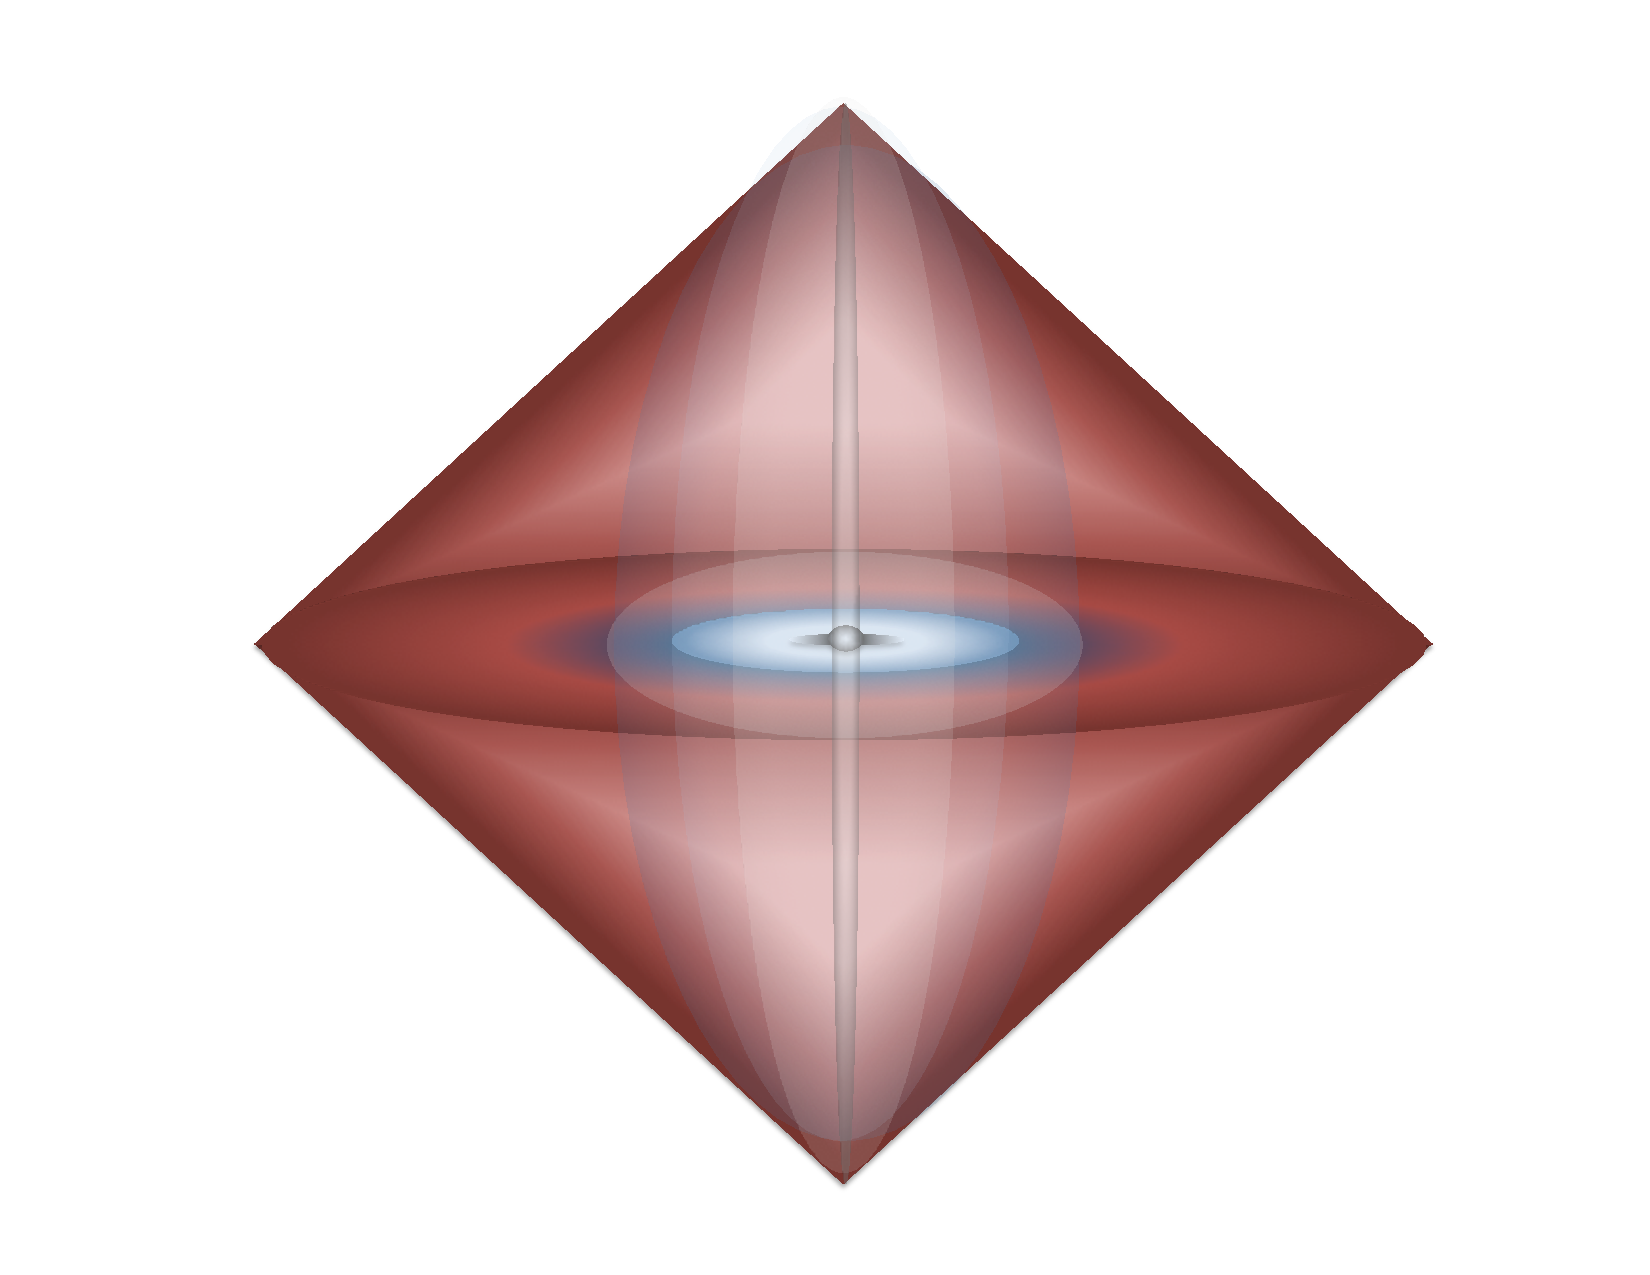
\includegraphics[scale=0.36]{ThermalStaticPatch.pdf}
\vspace{-1.0 cm}
\end{center}
\caption{\small \it The one-sided perspective on de Sitter space with a mass $M$ in the center. The entropy associated with the horizon area is contained in delocalized states that occupy the bulk. The mass $M$ removes part of, and therefore displaces, the entropy content in the interior.}
\end{figure}
 
 
 \subsection{An entropic criterion for the dark phase of emergent gravity}




 %In the following sections we adopt the one-sided perspective on de Sitter space, in which de Sitter entropy is seen as having a thermal origin. We postulate that the dark energy as well as the entropy content of de Sitter space is carried by excitations in the bulk space time. The reduction of the entropy content of de Sitter space due to matter is interpreted as being due to a transition from these thermal dark energy excitations to a localized form of energy. The expression (\ref{SMr}) corresponds to the local reduction of the entropy content of de Sitter space due to this transition. 
 


%The total entropy content $S(L)$ of de Sitter space is according to our postulate distributed over the volume of spacetime. This means that a subregion of de Sitter space contains a fraction of the total entropy that is proportional to its volume. %In the one sided view of de Sitter space, where one only considers a single static coordinate patch, the distribution of the entropy is to be homogeneous. By this we mean that in principle the entropy content of a subregion may depend on its distance from the horizon. 
Consider a spherical region with radius $r$ that is close to the center of the de Sitter static patch. According to our hypothesis in section \ref{sec:darkenergyandentropy} the  de Sitter entropy inside a spherical region with radius $r$  is given by  
\be
 \label{fracrS}
 S_{DE}(r)  = {1\over V_0} V(r) = {r\over L} {A(r)\over 4G\hbar}.
 \ee
 %This result is uniquely fixed once we require that the right hand side is proportional to the volume, and when we put $r=L$ that we obtain the full de Sitter entropy $S(L)$. 
 Note that the same factor $r/L$ appears in this expression as in the ratio between the removed entropy $S_M(r)$ within a radius $r$ and the total removed entropy $S_M(L)$. This observation has an important consequence and allows us to re-express the criterion mentioned in the introduction that separates the regimes where the `missing mass' becomes visible. We can now reformulate this criterion as a condition on the ratio between the removed entropy $S_M(r)$ and the entropy content $S_{DE}(r)$ of the dark energy. Concretely, the condition that $2\pi ML/\hbar$ is either 
 smaller or larger than $A/ 4G\hbar$ implies that 
\be
\label{criterion}
\big | S_M(r)  \big | \gtrless S_{DE}(r)\qquad\qquad{\mbox{or}} \qquad \qquad {2\pi M r\over \hbar}  \gtrless 
 {r\over L} {A(r)\over 4G\hbar} .
 \ee
 We can re-express this criterion as a condition on the volume $V_M(r)$ that contains the same amount of entropy that is taken away by the mass $M$ inside a sphere of radius $r$. This volume is given by
\be
\label{V0}
S_M(r) =-{1\over V_0} V_M(r)\qquad\qquad\mbox{with} \qquad\qquad V_0={4G\hbar L\over d-1}.
\ee
The criterion (\ref{criterion}) then becomes equivalent to the statement that the ratio 
of the volume $V_M(r)$ and the volume $V(r)$ of the ball of radius $r$ is smaller or larger than one 
\begin{equation}
\label{vareps}
\varepsilon_M(r) \equiv {V_M(r)\over V(r)} \ \gtrless \ 1	.
\end{equation}
%i.e.
%\begin{equation}
%\varepsilon(r) = {V_M(r)\over V(r)} %\gtrless 1.	
%\end{equation}
The observations on galaxy rotation curves therefore tell us that the nature of gravity changes depending on whether matter removes all or just a fraction of the entropy content of de Sitter.
One finds that the volume $V_M(r)$ is given by
\begin{equation}
\label{VMr}
V_M(r) = {8\pi G \over a_0} {M r\over d-1} 	.
\end{equation}
Here we replaced the Hubble length $L$ by the acceleration scale $a_0$ to arrive at a formula that is dimensionally correct. In other words, this volume does not depend on $\hbar$ or $c$. In fact, as we will see, the elastic description that we are about to present only depends on the constants $G$ and $a_0$ and hence naturally contains precisely those parameters that are observed in the phenomena attributed to dark matter. 

A related comment is that the ratio $\varepsilon_M(r)$ can be used to determine the value of the surface mass density $\Sigma_M(r) =M/A(r)$ in terms of $a_0$ and $G$ via
\begin{equation}
\label{Sigmaeps}
\varepsilon_M (r)	= {8\pi G\over a_0}   
 \Sigma_M(r) . %= {a_0\over 8\pi G}\varepsilon_M (r)
\end{equation}
This relation follows immediately by inserting the expressions (\ref{V0}) and the result 
(\ref{SMr}) for the removed entropy $S_M(r)$  into (\ref{vareps}). We also reinstated factors of the speed of light to obtain an expression that is dimensionally correct.  
 The regime where $S_M(r)< S_{DE}(r)$ corresponds to $\varepsilon_M(r) <1$, hence in this regime we 
 are dealing with low surface mass density and low gravitational acceleration.  
For this reason it will be referred to as the `sub-Newtonian' or `dark gravity' regime. 
 
 
 
  
 \subsection{Displacement of the entropy content of de Sitter space}
 
In the regime where only part of the de Sitter entropy is removed by matter, the remaining entropy contained in the delocalized de Sitter states starts to have a non-negligible effect. This leads to modifications to the usual gravitational laws, since the latter only take into account the effect of the area law entanglement. To determine these modifications we have to keep track of the displacement of the entropy content due to matter.  In the present context, where we are dealing with a central mass $M$ we can represent this displacement as a scalar function $u(r)$ that keeps track of the distance over which the 
information is displaced in the radial direction. 

In an elastic medium one encounters a purely radial displacement $u(r)$ when one removes (or adds) a certain amount of the medium in a symmetric way from inside a spherical region. 
The value of the displacement field $u(r)$ determines how much of the medium has been removed. If we assume that the medium outside of the region where the volume is removed is incompressible, the change in volume is given by that of a thin shell with thickness $u(r)$ and area $A(r)$. The sign of $u(r)$ determines whether the change in volume was positive or negative. 
We further assume that the change in volume is proportional to the removed entropy $S_M(r)$.  In this way we obtain a relation of the form
\be
\label{removedvolume}
S_M(r) ={1\over V^*_0} \, u(r)A(r)%\qquad\qquad\mbox{with} \qquad\qquad V^*_0={4G\hbar L\over d-2}.
\ee
where the volume $V_0^*$ is assumed to be of the same order as the volume $V_0$ per unit of 
entropy. To determine the value of $V_0^*$ we impose that at the horizon the displacement $u(L)$ is 
identified with the shift of the position of the horizon: $u(L) =\Phi(L)/ a_0$.   
From the fact that the removed entropy $S_M(r)$ is linear in $r$ we deduce that the displacement $u(r)$ falls off like $1/r^{d-3}$ just like Newton's potential $\Phi(r)$. This means that at an arbitrary radius $r$ we can express $u(r)$ in terms of $\Phi(r)$ as
\be
\label{u(r)}
u(r) = {\Phi(r)L}.
\ee
By combining the expressions (\ref{SMr}) and (\ref{u(r)}) and inserting the explicit form of the 
Newtonian potential (\ref{Phi(r)}) one finds that the volume $V_0^*$ is slightly larger than $V_0$
\be
\label{d-1/d-2}
V_0^*= {4G\hbar L \over d-2}\qquad\qquad\mbox{hence}\qquad \qquad {V_0^*\over V_0} = %\left(
{d -1\over d- 2}\, . %\right)  
\ee
%To determine the displacement $u(r)$ at other values of the radius we make use of the fact that the 
%removed  removed volume is proportional to the entropy $S_M(r)$ that has been removed. Hence, 
%\be
%{S_M(r)\over S_M(L)}= {u(r) A(r)\over u(L) A(L)} = {r\over L}
%{u(r)A(r)\over u(L)A(L)} = {S_M(r) \over S_M(L)} ={r\over L}
%\left({L\over r}\right)^{d-3} u(L) 
%\ee
%Each unit of removed entropy thus reduces the volume of the medium by an amount $V_0^*$ 
%that is a factor $(d-1)/(d-2)$ larger than the volume $V_0$ that contains one unit of entropy. 
The total removed volume is therefore slightly larger than $V_M(r)$ by the same factor.
We will denote the volume that has been removed from inside a spherial region ${\cal B}(r)$
by $V_M^*(r)$. 
The displacement $u(r)$ can thus be written  as
\begin{equation}
\label{urV}
u(r) = -{V_M^*(r)\over A(r)}	\qquad\qquad\mbox{where}\qquad\qquad
%\end{equation}
%where the removed volume $V_M^*(r)$ is given by  
%\begin{equation}
V^*_M(r) = {8\pi G \over a_0} {M r\over d-2} \, .
%\qquad\qquad\mbox{hence}\qquad\qquad 
%{V^*_M(r)\over V_M(r)} = 
%{d -1\over d- 2} %\right)  
% V_M(r) =  {8\pi G \over a_0} {M r\over d-1} 
\end{equation}
The relative factor between $V_M^*(r)$ and $V_M(r) $ can be directly traced back to the fact that we 
are dealing with a transition from area law to volume law entanglement. 
%This factor can also be understood from a more microscopic description \cite{toappear}. 

%As will become clear, the same factor $(d-1)/(d-2)$  also plays a natural role in the elastic 
%description. 



 \begin{figure}[btp]
\begin{center}
\vspace{-1.2 cm}
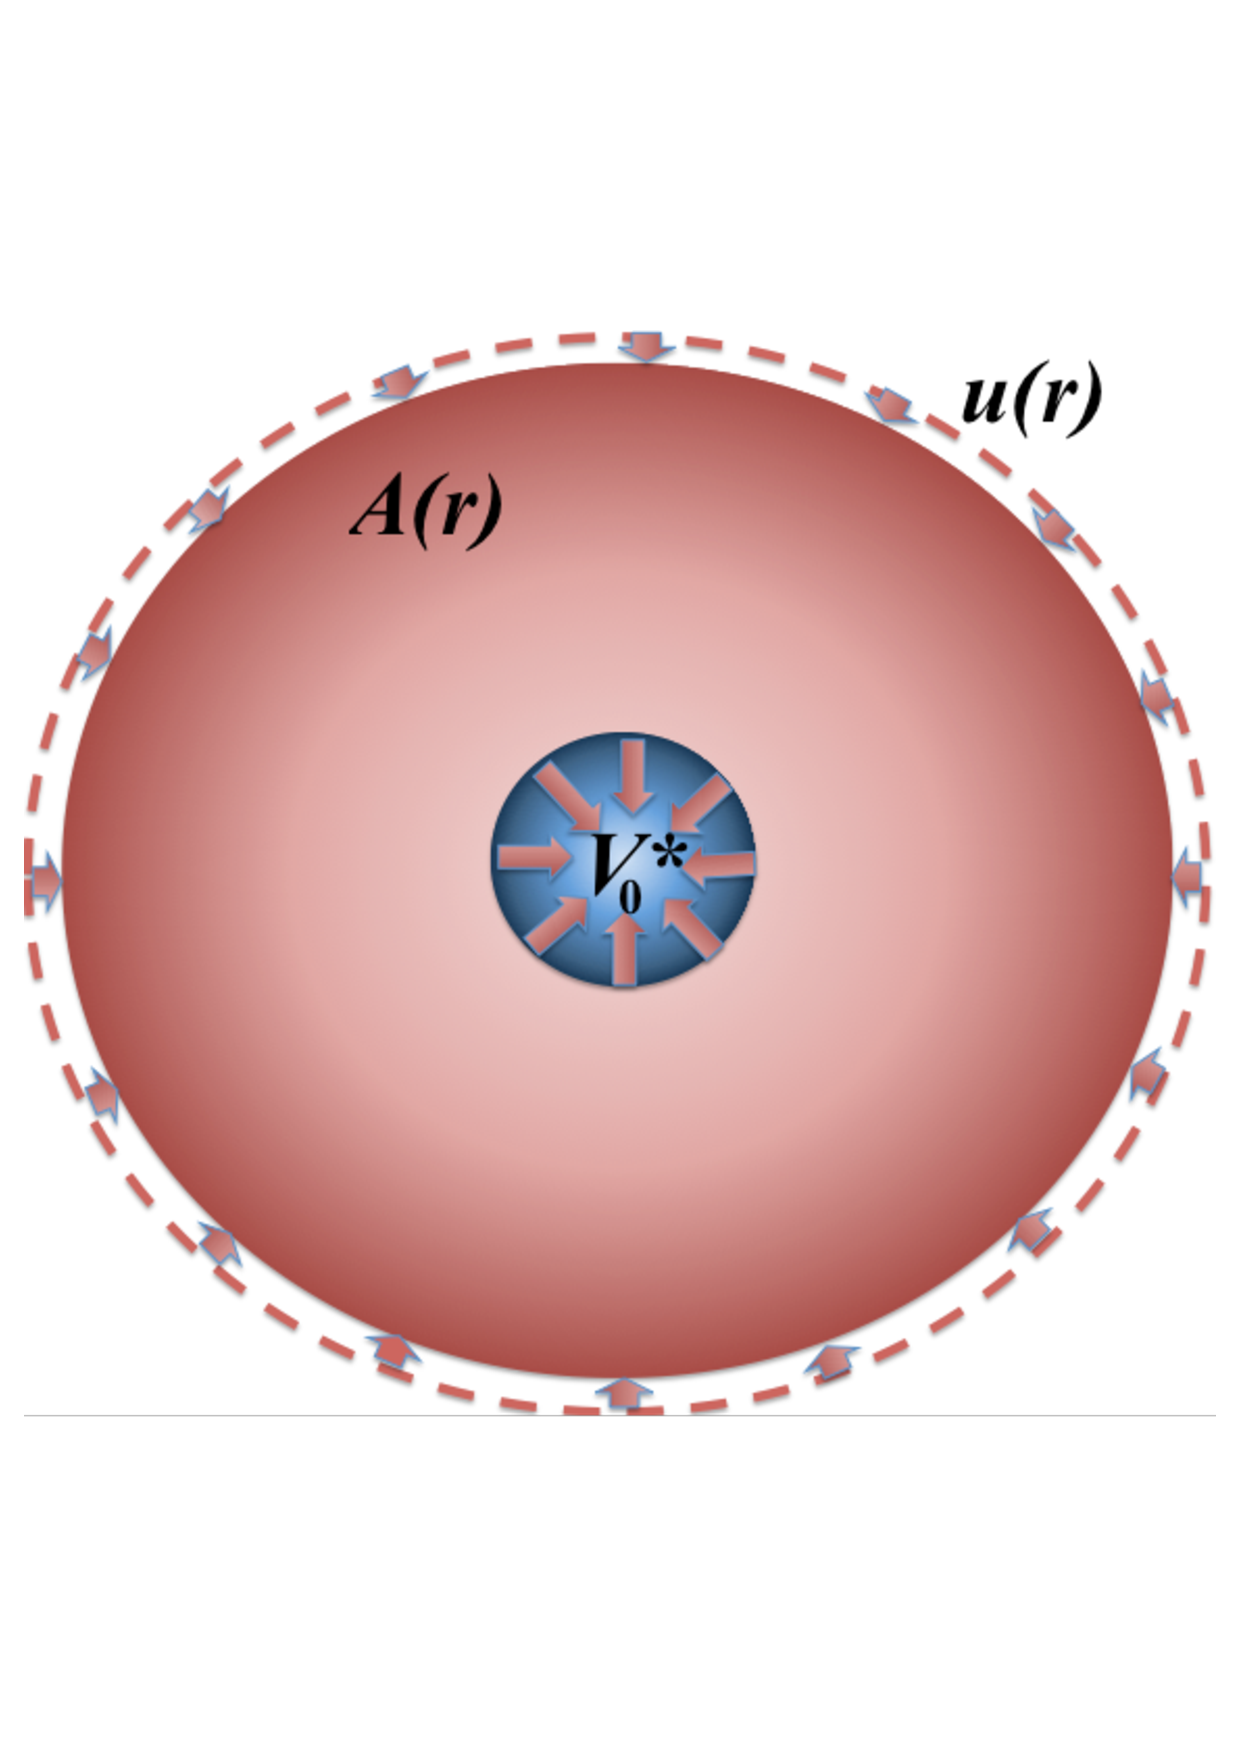
\includegraphics[scale=0.30]{Displacement2.pdf}
\vspace{-2.0 cm}
\end{center}
\caption{\small \it When a certain amount of volume $V_0^*$ is being removed from an incompressible elastic medium it leads to a displacement $\ u(r) = -V_0^*/A(r)$.}
\end{figure}
 

In a elastic medium a displacement field leads to an elastic strain
and corresponding stress, which in general are described by tensor 
valued fields. For the present discussion we are only interested in 
the normal components of the strain and the stress, hence to simplify our notation we will suppress tensor indices and denote the normal strain and normal stress simply by $\varepsilon(r)$ and $\sigma(r)$. 
%In the spherically symmetric 
%case we may assume that to a good approximation the radial direction corresponds to the direction of the largest normal strain and stress. 
Our proposed explanation of the gravitational phenomena associated to `dark matter' is  that in the regime where only part of the entropy is removed, that is where $\varepsilon_M(r)\!<\!1$,  the remaining entropy associated to the dark energy behaves as an {\it incompressible} elastic 
 medium.    Specifically, we propose that the entropy $S_M(r)$ is only removed from a local inclusion region ${\cal V}_M(r)$ with volume $V_M(r)$.   We represent the region ${\cal V}_M(r)$ as the intersection of a fixed region ${\cal V}_M(L)$ with 
a ball ${\cal B} (r)$ with radius $r$ centered around the origin, 
 \begin{equation}
 {\cal V}_M(r) ={\cal V}_M(L)\cap {\cal B}(r).	
 \end{equation}
 The precise shape or topology of the region ${\cal V}_M(L)$ will not be important for our 
 discussion. 
 
To deal with the fact that the removed volume $V^*_M(r)$ depends on the radius $r$, 
 we make use of the linearity of elasticity to decompose the region ${\cal V}_M(r)$ in 
 small ball-shaped regions ${\cal B}_i$ with volume $N_iV_0$.  From each ${\cal B}_i$ a fixed volume $N_i V^*_0$ has been removed corresponding to $N_i$ units of entropy. We first determine the displacement for each region, and then compute the total displacement by adding the different contributions.  
  
 Let us consider the displacement field $u(r)$ resulting from the  removal of a volume $NV_0^*$ from a single ball-shaped region ${\cal B}_0$ with volume $NV_0$.  For simplicity and definiteness, let us assume that ${\cal B}_0$ is centered at the origin of de Sitter space.  The displacement field outside of ${\cal B}_0$ is given by
\begin{equation}
\label{u(r)0}
u(r) = -{NV_0^*\over A(r)}.	
\end{equation}
The normal strain $\varepsilon(r)$ corresponds to the $r$-$r$ component of the strain tensor and is given by the radial derivative $\varepsilon(r) = u'(r)$. Hence
\begin{equation}
\label{epsilon}
\varepsilon(r) = {NV_0\over V(r)} . 
\end{equation}
Here we absorbed a factor $(d-2)/(d-1)$ by making the substitution $V_0^* \to V_0$.  
Since the volume of ${\cal B}_0$ is equal to $NV_0$, we find that the normal strain $\varepsilon(r)$ at 
its boundary is precisely equal to one. Note that to obtain this natural result we made use of the specific ratio of $V_0^*$ and $V_0$. 


This same calculation can be performed for each small ball ${\cal B}_i$ and leads to a displacement field  
$u_i$ and strain $\varepsilon_i$ identical to (\ref{u(r)0}) and (\ref{epsilon}) where the radius is defined 
with respect to the center of ${\cal B}_i$ and the number of units of removed entropy is equal to $N_i$.  By adding all these different contributions we can in principle determine the total displacement and strain due to the removal of the entropy $S_M(r)$ from the region ${\cal V}_M$.  Here we have to distinguish two regimes. When $V_M(r) >V(r)$ we are inside the region ${\cal V}_M$ and `all the available volume' has been removed. This means, the entropy reduction due to the mass is larger than the available thermal entropy. In this region the response to the entropy reduction due to the mass $M$ is controlled by the area law entanglement, which leads to the usual gravity laws. We are interested in the other regime where $V_M(r) < V(r)$, since this is where the modifications due to the volume law will appear. 

 The total amount  of entropy that is removed within a radius $r$ is equal to $S_M(r)$. 
 Hence, at first we may simply try to replace $N$ by $S_M(r)$ so that the removed volume $NV^*_0$ becomes equal to $V_M^*(r)$, and $NV_0$ to the volume $V_M(r)$ of the region ${\cal V}_M(r)$. Indeed, if we make the substitutions
\begin{equation}
\label{substitute}
NV^*_0\ \longrightarrow\ V^*_M(r)	\qquad\qquad\mbox{and}\qquad\qquad NV_0\ \longrightarrow\  V_M(r)
\end{equation}  
the displacement $u(r)$ becomes equal to (\ref{urV}) and the expression (\ref{epsilon}) for $\varepsilon(r)$  becomes identical to the quantity $\varepsilon_M(r)$ introduced in (\ref{vareps}). In other words, we find that the apparent DM criterion can be interpreted as a condition on the normal elastic strain $\varepsilon(r)$: the transition from standard Newtonian gravity to the apparent dark matter regime occurs when the elastic strain drops in value below one.  

%In our derivation of (\ref{epsilon}) we took the derivative of  (\ref{u(r)0}) while keeping the volume 
%$NV^*_0$ constant. If we would compute the normal strain directly from (\ref{urV}) we would 
%also have to differentiate $V^*_M(r)$ with respect to $r$. This would lead to a results that differs  from (\ref{epsilon}) after the substitution (\ref{substitute}) by a factor $(d-3)/(d-2)$.   
The quantity $\varepsilon(r)$, as we have now defined it, equals the normal strain in the regime where the removed volume is kept constant: in other words, where the medium is treated as incompressible. As we will explain in more detail  in section 7,  in this regime the normal strain $\varepsilon(r)$ %is proportional to the normal stress $\sigma(r)$ and 
    determines the value of the apparent surface mass density $\Sigma(r)$ precisely through the relation (\ref{Sigmaeps}), which for convenience we repeat here in slightly different form
\begin{equation}
\label{Sigmeps}
\Sigma(r) =  {a_0\over 8\pi G}\,\varepsilon(r) .
\end{equation}
In the next subsection we will use this relation to determine the apparent surface mass density in the regime $\varepsilon(r) <1$.  Here the volume $V_M(r)$ is smaller than the volume $V(r)$ of the sphere with radius $r$. Hence, it is not clear anymore that one can simply take the relation (\ref{epsilon}) and make the substitution (\ref{substitute}).  A more precise derivation would involve adding all these separate contributions of the small balls ${\cal B}_i$ that together compose the region ${\cal V}_M(r)$.  We will now show that this leads through the relation (\ref{Sigmeps}) to a surface mass density that includes the contribution of the apparent dark matter.  


%We like to point out that irrespective of issues of normalization and other details, that the arguments that we have presented so far already give a natural explanation for the observed universal value $a_0/8\pi G$ of the surface mass density of `dark matter'. 
%Indeed, as we will see in the following section, the normal strain is actually related to the gravitational acceleration $g(r)=\Phi'(r)$.  via $g(r) = a_0\varepsilon(r)$, while the surface mass density $\Sigma(r)$ is determined by the normal stress $\sigma(r)$ through the following simple



 %via 
%\begin{equation}
%\Sigma(r) ={\sigma(r)\over a_0} 
%= {a^2_0\over 8\pi G} \varepsilon(r) \qquad \qquad \mbox{hence} \qquad \qquad  
%{\sigma(r) = \Sigma(r) a_0}
%\end{equation}
 


%In this regime the normal stress $\sigma(r)$ is proportional to the normal strain $\varepsilon(r)$ with the constant of proportionality given by the shear modulus. In the next section we will determine the value of the shear modulus in terms of the constants $G$ and $a_0$, and derive the following simple relation between the normal stress and apparent surface mass density 
%\begin{equation}
%\sigma(r) = {a^2_0\over 8\pi G} \varepsilon(r) \qquad \qquad \mbox{hence} \qquad \qquad  
%{\sigma(r) = \Sigma(r) a_0}
%\end{equation}




%XXXXXXXX


%The microscopic explanation is 
%that the transition that forms the mass $M$ actually removes more excitations from the dark energy 
%medium than one would conclude purely on the basis of the entropy reduction $S_M(L)$. This will be 
%further explained in section 8 and in the appendix.  

   



\subsection{A heuristic derivation of the Tully-Fisher scaling relation }  
 
After having introduced all relevant quantities, we are now ready to present our proposed explanation of the observed phenomena attributed with dark matter.   It is based on the idea that the standard laws of Newton and general relativity describe the response of the area law entanglement to matter, while in the regime $\varepsilon(r)\!<\!1$ the gravitational force is dominated by the elastic response due to the volume law contribution. We will show that the Tully-Fisher scaling law for the surface mass densities of the apparent dark matter and the baryonic matter is derived from a quantitive estimate of the strain and stress caused by the entropy $S_M(r)$ removed by matter. 



Let us go back to the result (\ref{epsilon}) for  the strain outside a small region ${\cal B}_0$ of size $NV_0$,  %from which we removed a fixed given volume $NV_0^*$
and let us compute the integral of the square $\varepsilon^2(r)$ over the region outside of ${\cal B}_0$ with $V(r)> NV_0$.  
We denote this region as the complement $\overline{{\cal B}}_0$ of the ball ${\cal B}_0$.  The integral is easy to perform and simply gives the volume of the region ${\cal B}_0$ from which the entropy was removed
\begin{equation}
\label{epsilon2}
\int_{\strut {\overline{\cal B}_0}}\varepsilon^2(r) A(r) dr =\int_{NV_0}^\infty  \left({NV_0\over V}\right)^2 dV = NV_0.
\end{equation}
This result is well known in the theory of `elastic inclusions' \cite{Eshelby}.   In this context equation (\ref{epsilon2}) is used to estimate the elastic energy caused by the presence of the inclusion. This same method has also been applied to calculate memory effects in entangled polymer melts \cite{RubOb}.
 
We can repeat this calculation for all the small balls ${\cal B}_i$ that together make up the region ${\cal V}_M(r)$ to show that the integral of $\varepsilon_i^2$ over the region outside of ${\cal B}_i$ is given by $N_iV_0$.  Since $\varepsilon_i$ quickly falls off like $1/r^{(d-1)}$ with the distance from the center, the main contribution to the integral comes from the neighbourhood of ${\cal B}_i$.   
We now assume that, in the regime where $V_M(r)<V(r)$,   all the small regions ${\cal B}_i$ are disjoint, and are separated enough in distance so that the elastic strain $\varepsilon_i$ for each ball ${\cal B}_i$ is primarily localized in its own neighbourhood.  This means that the integral of the square of the total strain is equal to the sum of the contributions of the individual squares $\varepsilon_i^2$ for all the balls ${\cal B}_i$. In other words, the cross terms between $\varepsilon_i$ and $\varepsilon_j$ can be ignored when $i\neq j$. In section 7 we will show that this can be proven to hold exactly.  The integral of $\varepsilon^2$ over the ball ${\cal B}(r)$ with radius $r$ thus decomposes into a sum of contributions coming from the neighbourhoods of each small region ${\cal B}_i$
\begin{equation}
\int_{\strut {{\cal B}(r)}}\!\!\!\!\varepsilon^2 dV  \, \approx\,  \sum_i \int_{\strut {\overline{{\cal B}}_i \cap \cal B}(r) }\!\!\!\!\!\varepsilon_i^2 dV \,\approx\, \sum_{{\cal B}_i \subset  {\cal B}(r)} \int_{\strut {\overline{{\cal B}}_i} }\!\!\varepsilon_i^2 dV \,  =\, \sum_{{\cal B}_i \subset  {\cal B}(r)}  \!\!N_iV_0 = V_M(r) . 
\end{equation}
Each of these integrals is to a good approximation equal to the volume $N_i V_0$ of ${\cal B}_i$, and since these together constitute the region ${\cal V}_M$, we find that the total sum gives the volume $V_M(r)$.  We will further make the simplifying assumption that in the spherically symmetric situation   the resulting strain is just a function of the radius $r$.  In this way we find 
\begin{equation}
\label{epsilon4}
%\int_{\strut {{\cal B}(r)}}\!\!\!\!\varepsilon^2 dV  = 
\int_0^r \!\!\varepsilon^2(r') A(r') dr' 
= V_M(r) .
\end{equation}
%\begin{equation}
%\label{epsilon4}
%\int_{\strut {{\cal B}(r)\cap \overline{{\cal B}}(r_0)} }\!\!\!\!\!\!\!\!\!\varepsilon^2 dV  = \int_{r_0}^r \!\varepsilon^2(r) A(r) dr 
%= V_M(r)-V_M(r_0)
%\end{equation}
To arrive at the Tully-Fisher scaling relation between the surface mass density of the 
apparent dark matter and the baryonic dark matter we differentiate this expression with respect to the 
radius.  If we assume that the mass distribution is well localised near the origin,  we can treat the mass 
$M$ as a constant. In that case we obtain
\begin{equation}
\varepsilon^2(r) =
{1\over A(r)} {dV_M(r)\over dr}  = {1\over A(r)} {8\pi G \over a_0} {M\over {d-1}}
\end{equation}
We now make the identification of the apparent surface mass density with $\varepsilon(r)$. We obtain
a relationship for the square surface mass density of the apparent dark matter and surface mass density 
of the visible baryonic matter. To distinguish the apparent surface mass density from the one defined in terms of the mass $M$ we will denote the first as $\Sigma_D$ and the latter as $\Sigma_B$. These quantities are defined as
\begin{equation}
\Sigma_D(r) = {a_0\over 8\pi G} \,\varepsilon(r) \qquad \qquad \mbox{and}\qquad \qquad \Sigma_B(r) = {\! M\,\over \ A(r)} .
\end{equation}
With these definitions we precisely recover the relation
\begin{equation}
\Sigma_{D}(r)^2 = {a_0\over 8\pi G} {\Sigma_B (r)\over d-1}	 .
\end{equation}
which was shown to be equivalent to the Tully-Fisher relation. 
 
 In the remainder of this paper we will again go over the arguments that lead us to the proposed elastic phase of emergent de Sitter gravity and further develop the correspondence between the familiar gravity laws and the tensorial description of the elastic phase. In particular, we will clarify the relation between the elastic strain and stress and the apparent surface mass density. We will also revisit the derivation of the Tully-Fisher scaling relations and present the details of the calculation at a less heuristic level. This will clarify under what assumptions and   conditions this relation is expected to hold. 





\section{The First Law of Horizons and the Definition of Mass}
\setcounter{equation}{0}






%\subsection{The first law of horizon thermodynamics.}


Our goal in this section is to understand the reduction of the de Sitter entropy due to matter in more detail. For this purpose we will make use of Wald's formalism \cite{WaldNoether} and methods similar to those developed in \cite{Raamsdonketal, Swingle-vR, Jacobson2} for the derivation of the (linearized) Einstein equations from the area law entanglement.  We will generalise some of these methods to de Sitter space and discuss the modifications that occur in this context. Our presentation closely follows that of Jacobson \cite{Jacobson2}.  

\subsection{Wald's formalism in de Sitter space}

In Wald's formalism \cite{WaldNoether} the entropy associated to a Killing horizon is expressed as the Noether charge for the associated Killing symmetry.  For Einstein gravity the explicit expression is\footnote{Here we use the notation of \cite{Raamsdonketal} by introducing the symbol ${\bf\epsilon}_{ab}= {1\over (d-2)!}\epsilon_{abc_1\ldots c_{d-2}} dx^{c_1}\!\wedge\!\ldots \!\wedge\! dx^{c_{d-2}}$.} 
\be
\label{Noether}
{\hbar\over 2\pi} S = \int_{hor}\!\! Q[\xi] = -{1\over 16\pi G} \int_{hor}\!\!\nabla^a \xi^b {\mathbf \epsilon}_{ab} .
\ee
Here the normalization of the Killing vector $\xi^a$ is chosen so that $S$   precisely  equals $A/4 G\hbar$, where $A$ is the area of 
the horizon.  When there is no stress energy in the bulk, the variation $\delta Q[\xi]$ of the integrand can be extended to a closed form by imposing the (linearized) Einstein equations for the (variation of) the background geometry.  For black holes this fact is used to deform the integral over the horizon to the boundary at infinity, which leads to the first law of black hole thermodynamics. 

These same ideas can be applied to de Sitter space. Here the situation is `inverted' compared to the black hole case, since we are dealing with a cosmological horizon and there is no asymptotic infinity.
In fact, when there is no stress energy in the bulk the variation of the horizon entropy vanishes, since there is no boundary term at infinity.  The first law of horizon thermodynamics in this case reads \cite{Jacobson2, Gibbons-Hawking}
\be
\label{desitter1stlaw}
{\hbar \over 2\pi}\delta S +\delta H_\xi=0
\qquad\qquad\mbox{where}
\qquad\qquad
\delta H_\xi  = \int_{\cal C} \xi^a T_{ab} \, d\Sigma^b
\ee
represents the variation of the Hamiltonian associated with the Killing symmetry. It is expressed as an 
integral of the stress energy tensor over the Cauchy surface $\cal C$ for the static patch. We are interested in a situation where the stress is concentrated in a small region around the origin, with a radius $r_\infty$ that is much smaller than the Hubble scale. This means that the integrand of $\delta H_\xi$ only has support in this region. Furthermore, the variation $\delta Q[\xi]$ of integrand of the Noether charge can be extended to a closed form almost everywhere in the bulk, except in the region with the stress energy. This means we can deform the surface integral over the horizon to an integral over a surface ${\cal S}_\infty$ well outside the region with the stress energy.  Following Wald's recipe we can write this integral as 
\be
\label{deltaK}
 {\delta H_\xi }  = \int_{{\cal S}_\infty}\!\! \bigl(\delta Q[\xi] -\xi\!\cdot\delta B\bigr) 
\ee
where we included an extra contribution $\xi\!\cdot\delta B$ which vanishes on the horizon. 






The Hamiltanian $H_\xi$ is proportional to the generator of time 
translations in the static coordinates of de Sitter space, where the constant of proportionality given by the surface gravity $a_0$ on the cosmological horizon. Hence we have
\be
\label{KtoM}
\xi^a{\partial\over \partial x^a} = {1\over a_0} {\partial\over \partial t}  \qquad\qquad\mbox{ which implies}\qquad\qquad  \delta H_\xi ={\delta M\over a_0}, 
\ee
where $\delta M$ denotes the change in the total mass or energy contained in de Sitter space. 
With this identification the first law takes an almost familiar form
\be
T \delta S = -\delta M   \qquad\qquad\mbox{with}\qquad\qquad   T={\hbar a_0 \over 2\pi}.
\ee
The negative sign can be understood  as follows. In deforming the Noether integral (\ref{Noether}) from the horizon to the surface ${\cal S}_\infty$  %Note that the same mass $M$ has to appear on both sides of the cosmological horizon,  because the Noether charges on both sides can be deformed into another. 
 we have to keep the same orientation of the integration surface.  However, in the definition of the 
 mass the normal points outward, while the opposite direction is used in the definition 
 of the entropy. 
   
%, where it takes the form
%horizon.  % it can be identified with the known ADM expression for the variation of the mass $M$ of the black hole 
%One can thus make the following identification
%\be
%\bigl\langle {\delta K} \bigr\rangle = \int_\infty\!\! \bigl(\delta Q[\xi_K] -\xi_K\!\cdot\delta B\bigr) ={\delta M\over \kappa}
%\ee

\subsection{An approximate ADM definition of mass in de Sitter} 

We would like to integrate the second equation in (\ref{KtoM}) to obtain a definition of the mass $M$ similar to the ADM mass. Strictly speaking, the ADM mass can only be defined at spatial infinity. However, suppose we choose the radius $r_\infty$ that defines the integration surface ${\cal S}_\infty$  to be ({\it i}) sufficiently large so that the gravitational field of the mass $M$ is extremely weak, and ({\it ii})  small enough so that $r_\infty$ is still negligible compared to the Hubble scale $L$.  In that situation it is reasonable to assume that to a good approximation one can use the standard ADM expression for the mass.  By following the same steps as discussed in \cite{WaldNoether,Iyer-Wald} for the ADM mass, we obtain the following surface integral expression for the mass  $M$ \cite{ADM,Waldbook}
\be
\label{ADM}
M = \int_{{\cal S}_\infty}\! \left ( Q[t] - t \cdot B \right) =  {1\over 16\pi G} \int_{S_{\infty}}\! \bigl( \nabla_j h_{ij}-\nabla_i 
h_{jj} \bigr)dA_i.
\ee
Here $h_{ij}$ is defined in terms of the spatial metric. 
%The derivation of the linearized 
%Einstein equations in AdS is based on these same steps, but in reversed order. One assumes the first law, and then concludes that the form inside the integral (\ref{deltaK}) must be closed.


 

%We can derive the sign in this equation using the formal steps of Wald's derivation. Let us imagine  putting a finite but small mass $M$ in the center of the static patch.    


%Another way of understanding the difference in sign is that the entropy associated with the cosmological horizon can not be changed by `throwing in matter from infinity', like one can do for black holes in flat space or AdS. Instead, to increase the entropy of the de Sitter horizon when has to let matter that already exist inside the cosmological horizon pass though it. The entropy increase of the cosmological horizon is thus related to the decrease of the mass inside the enclosed causal region, or vice versa. 


%In \cite{Jacobson2} it was argued following \cite{GibbonsHawking2} that empty de Sitter space should be viewed as a vacuum state with maximal entropy, since it represents a state at `entanglement' equilibrium. We %take a different point of view and 
%The fact that the entropy decreases when we increase the Killing energy seems to support the interpretation that de Sitter space is a state with maximal entropy, and hence corresponds to a microscopic state that is in thermal equilibrium. 


 
 
 
We assume now that we are in a Newtonian regime in which  Newton's potential $\Phi$ is much smaller than one, and furthermore far away from the central mass distribution so that $\Phi$ depends only on the distance to the center of the mass distribution. In this regime the metric takes the following form\\[-2mm]
\be
\label{approxmetric}
%\lim_{|x|\to\infty} \,
%\Bigl\lbrack ds^2
%\Bigr \rbrack
ds^2_{\, \strut|x|= r_{{}_\infty}}= 
%ds^2 \  \longrightarrow {}_{{}_{\strut \!\!\!\!\!\!\!\!\!\!\!\!\!\!\!\!\!\!\!|x|\to\infty}} \  
-dt^2 +dx_i^2 - 2\Phi(x) \Bigl(dt^2+{\left(x_i dx_i\right)^2\over |x|^2}\Bigl) .
 \ee
We will assume that the matter is localized well inside the region $|x|< r_{{}_\infty}$. This means that the Newtonian potential is in good approximation only a function of the radius.
 When we insert the spatial metric\\[-2mm]
 \be 
 h_{ij} = \delta_{ij}-2\Phi(x) n_i n_j \qquad\quad\mbox{with}\qquad\quad n_j \equiv {x_j\over |x|}
 \ee 
 into the ADM integral (\ref{ADM}) and choose a spherical surface with a fixed radius $r_{{}_\infty}$ we find the following expression for the mass 
\be
\label{ADMPhi}
M%={1\over 8\pi G} \int_{\infty}\!  \Bigl( n_i\nabla_i \Phi- \nabla_i (\Phi n_i )\Bigr) dA
=-{1\over 8\pi G} \int_{r_\infty}\!\Phi(x) \nabla_j n_{j\,}  dA\ee
where $dA = n_i dA_i$. It is easy to check the validity of this expression using the explicit form of $\Phi(x)$ (\ref{Phi(r)}) and the fact that for a spherical surface\\[-2mm] 
\be
\nabla_jn_j = {d-2\over |x|}.\\[-2mm]
\ee
%In general the l.h.s. is related to the extrinsic curvature of the integration surface.  


%In general relativity the most precise definition of the enclosed mass is usually obtained by going to the most asymptotic region of space.  It is therefor natural to try to define the mass $M$ by the limit where we take $r_\infty$ all the way to the horizon. However, here we recover the Noether integral that defines the change in entropy. This suggests that the microscopic definition of the mass in de Sitter space is given by the relative entropy of the state with the mass and the state without the mass. However, as we pointed out, for this definition to work one has to take the state with the mass as the reference equilibrium state.

\vspace{1cm}

\section{The Elastic Phase of Emergent Gravity}
\setcounter{equation}{0}  
  
We now return to the central idea of this paper. As we explained, the effect of matter is to displace the entropy content of de Sitter space. Our aim is to describe in detail how the resulting elastic back reaction translates into an effective gravitational force. We will describe this response using the standard linear theory of elasticity.

\subsection{Linear elasticity and the definition of mass}

The basic variable in elasticity is the displacement field $u_i$. The linear strain tensor is given in terms of $u_i$ by
\be
\label{straindef}
\varepsilon_{ij} ={1\over 2}\left(\nabla_i u_j+ \nabla_j u_i\right). %= {\varepsilon_{kk}\over {d-1}} \delta_{ij}+\varepsilon'_{ij} %=\varepsilon^{dev}_{ij}+\varepsilon^{hyd}_{ij}
\ee
In the linear theory of elasticity the stress tensor $\sigma_{ij}$ obeys the tensorial version of Hooke's law. For isotropic and 
homogeneous elastic media there are two independent elastic moduli conventionally denoted by  $\lambda$ and $\mu$.    These so-called Lam\'{e} parameters appear in the stress tensor as follows
 \be
 \label{stress}
\sigma_{ij}= \lambda\, \varepsilon_{kk} \delta_{ij} + 2\mu\, \varepsilon_{ij} . %= \Bigl(\lambda + {2\mu\over d - 1 }\Bigr)\varepsilon_{kk}\delta_{ij}+ 2\mu \, \varepsilon'_{ij} 
 \ee 
The combination $K=\lambda + 2\mu/(d-1) $ is called the bulk modulus. The shear modulus is equal to $\mu$: it determines the velocity of shear waves, while the velocity of pressure waves is determined by $\lambda + 2\mu$.   Requiring that both velocities are real-valued leads to the following inequalities on the Lam\'e parameters 
\be
\mu \geq 0 \qquad \qquad \mbox{and}\qquad \qquad \lambda +2\mu\geq 0.
\ee
%where we assumed that the elastic medium has a positive mass density. 
Our aim is to relate all these elastic quantities to corresponding gravitational quantities.  In particular, we will give a map from the displacement field, the strain and the stress tensors to the apparent  Newton's potential, gravitational acceleration and surface mass density. In addition we will express  the elastic moduli in terms of Newton's constant $G$ and the Hubble acceleration $a_0$.

Since de Sitter space has no asymptotic infinity, the precise definition of mass is somewhat problematic. In general, the mass can only be precisely defined with the help of a particular reference frame. In an asymptotically flat or AdS space, this reference frame is provided by the asymptotic geometry. We propose that in de Sitter space the role of this auxiliary reference frame, and hence the definition of the mass, is provided by the elastic medium associated with the volume law contribution to the entanglement entropy.   In other words, the reference frame with respect to which we define the mass $M$ has to be chosen at the location where the standard Newtonian gravity regime makes the transition to the elastic phase. This implies that the definition of mass depends on the value of the displacement field and its corresponding strain and stress tensor in the elastic medium. 

We will now show that the ADM definition of mass can be naturally translated into an expression for the elastic strain tensor or, alternatively, for the stress tensor.  In section 4, we  
found that the displacement field $u_i$ at the horizon is given by
\be
\label{udef}
u_i = {\Phi\over a_0} n_i \qquad\qquad\mbox{with}\qquad\qquad n_i ={x_i\over |x|}
\ee 
and we argued that a similar identification holds in the interior of de Sitter space.  Alternatively, we can introduce the displacement field $u_i$ in terms of the spatial metric $h_{ij}$ via the Ansatz
\be
\label{hij}
h_{ij} =\delta_{ij} - {a_0\over c^2} \left(u_i n_j +n_i u_j\right) .
\ee
Eventually we take a non-relativistic limit in which we take $L$ and $c$ to infinity, while keeping 
$a_0 = c^2/L$ fixed.  Hence we will work almost exclusively in the Newtonian regime, and will not attempt to make a correspondence with the full relativistic gravitational equations. 


It is an amusing calculation to show that the expression (\ref{ADMPhi}) for the mass $M$ can be rewritten in the following suggestive way in terms of the strain tensor $\varepsilon_{ij}$ for the displacement field $u_i$ defined in (\ref{udef})
\be
\label{Mstrain}
M =  {a_0\over 8\pi G} \int_{{\cal S}_\infty} \bigl( n_j\varepsilon_{ij}-n_i \varepsilon_{jj} \bigr) dA_i \,.
\ee
In this calculation we used the fact that the integration surface is far away from the matter distribution,  so that $\Phi$ only depends on the distance $|x|$ to the center of mass.  This same result can be derived by inserting the expression (\ref{hij}) together with (\ref{udef}) into the standard ADM integral (\ref{ADM}). It is interesting to note that the first term corresponds to $Q[t]$ while the second term is equal to $-t \cdot B$.   We again point out that the prefactor $a_0/8\pi G$ in (\ref{Mstrain}) is identical to the observed critical value for the surface mass density. 



When we multiply the expression (\ref{Mstrain}) for    $M$ by the acceleration scale $a_0$ we obtain a physical quantity with the dimension of a force.  This motivates us to re-express the right hand side as 
\be
\label{Mstress}
M a_0 = \oint_{{\cal S}_{\infty}} \!\!\!\sigma_{ij} n_{j\,} dA_i
\ee
where we identified the stress tensor $\sigma_{ij}$ with the following expression in terms of the strain tensor 
\be
\label{sigmadef}
\sigma_{ij}  = {a_0^2\over 8\pi G}\bigl(\varepsilon_{ij}- \varepsilon_{kk}\delta_{ij}\bigr) .
\ee
By comparing with (\ref{stress}) we learn that the  elastic moduli of the dark elastic medium   take the following values
\be
\label{moduli}
\mu =  {a_0^2\over 16\pi G} \qquad \qquad \mbox{and}\qquad \qquad \lambda +2\mu = 0 .
\ee
We thus find that the shear modulus has a positive value, but that the P-wave modulus vanishes. 
The shear modulus has the dimension of energy density, as it should, and is up to a factor $
(d-1)(d-2)$ equal to the cosmological energy density.  

In the theory of elasticity the integrand of the right hand side of (\ref{Mstress}) represents the outward traction force $\sigma_{ij}n_j$. The left hand side on the other hand is the outward force on a mass shell with total mass $M$   when it experiences an outward acceleration equal to the surface acceleration $a_0$ at the horizon.  Hence,  it is natural to interpret the equation (\ref{Mstress}) as expressing a balance of forces. 

The precise value (\ref{moduli}) of the shear modulus is dictated by the following calculation. Let us consider the special situation in which the surface ${\cal S}_\infty$ corresponds to an equipotential surface. In this case we can equate the gravitational self-energy  enclosed by ${\cal S}_\infty$ exactly with the elastic self energy
\begin{equation}
{1\over 2} M\Phi = {1\over 2}	\oint_{{\cal S}_{\infty}} \!\!\!\sigma_{ij} u_{j\,} dA_i  \, .
\end{equation}
%This is one of the many correspondence relations between the elastic and 
 In the next subsection we further elaborate these correspondence rules between the elastic phase  and the Newtonian regime of emergent gravity. Specifically, we will show that the elastic equations naturally lead to an effective Newtonian description in terms of an apparent surface mass density.  






\subsection{The elasticity/gravity correspondence in the sub-Newtonian regime}


 First we start by rewriting the familiar laws of Newtonian gravity in terms of a surface mass density vector.  
We introduce a vector field $\Sigma_i$ defined in terms of the Newtonian potential $\Phi$ via
\be
\label{Sigmadef}
\Sigma_i =  -\left( {d-2\over d-3}\right) {g_i \over  8\pi G}  \qquad\qquad
%\be
%\Sigma_i \equiv  -\left( {d-2\over d-3}\right) {1 \over  8\pi G}  %\, g_i\qquad\qquad \mbox{where} \qquad \qquad g_i =- 
%\nabla_i\Phi
%\ee
\mbox{where}\qquad\qquad
g_i =-\nabla_i\Phi
\ee 
is the standard gravitational acceleration. By working with $\Sigma_i$ instead of $g_i$ we avoid some annoying dimension dependent factors, and make  the correspondence with the elastic quantities more straightforward. The normalization is chosen so that the gravitational analogue of Gauss' law  
%and d-dimensional Poisson equation for the Newtonian potential  
simply reads
\be 
\nabla_i \Sigma_i = \rho  \qquad\qquad\mbox{or}\qquad\qquad \oint_{\cal S}  \Sigma_i \, dA_i = M 
\ee
where $M$ is the total mass inside the region enclosed by the surface $\cal S$.  
We will refer to $\Sigma_i$ as the surface mass density. The gravitational self-energy of a mass configuration can be expressed in terms of the acceleration field $g_i$ and the surface mass density vector field $\Sigma_i$ as
\begin{equation}
U_{grav} ={1\over 2} \int \!dV g_i \Sigma_i	 .
\end{equation}
We are interested in the force on a small point mass $m$ located at some point $P$. Its Newtonian potential $\Phi^{(m)}$ and surface mass density $\Sigma^{(m)}$ are sourced by the mass density  $\rho^{(m)}=m\,\delta(x\!-\!x_P)$. The force that acts on the point mass is derived from the gravitational potential, which obeys the representation formula
\begin{equation}
m \Phi(P) = \oint_{\cal S} dA_i \left(  \Phi^{(m)} \Sigma_i  -  \Phi \,  \Sigma_i^{(m)} \right) .
\end{equation}
Here the surface $\cal S$ is chosen so that it encloses  the mass distribution that sources the field $\Phi$ and $\Sigma_i$. 


%sand are expressed in tems of the Green's function of the $(d-1)$-dimensional Laplacian.   


All these equations have direct analogues in the linear theory of elasticity.  The displacement field $u_i$ is analogous to the Newtonian potential $\Phi$,  the strain tensor $\varepsilon_{ij}%={1\over 2} (\nabla_i u_j+\nabla_j u_i)
$ plays a similar role as the gravitational acceleration $g_i %=-\nabla_i\Phi
$, and the stress tensor $\sigma_{ij}$ is the direct counterpart of the surface mass density $\Sigma_i$.  
For instance,  our definition (\ref{Sigmadef}) of the surface mass density $\Sigma_i$ is the direct analogue of the definition (\ref{stress}) of the stress tensor $\sigma_{ij}$, with the obvious correspondence between the expressions for $g_i$ in terms of $\Phi$ and $\varepsilon_{ij}$ in terms of  $u_i$.  The counterparts of the Poisson equation and Gauss' law read\\[-1mm]
\be
\nabla_i \sigma_{ij}+b_j  = 0 \qquad \qquad\mbox{and} \qquad \qquad \oint_{\cal S} \sigma_{ij} \,dA_j + F_i =0\\
\ee 
where the body force $b_j$ represents the force per unit of volume that acts on the medium and $F_j$ is the total force acting on the part of the medium enclosed by the surface ${\cal S}$. Also the elastic energy is given, except for the sign, in a completely analogous way 
\begin{equation}
U_{elas} ={1\over 2} \int \!dV \varepsilon_{ij} \sigma_{ij}	 .
\end{equation}
The elastic equivalent of the point mass is a point force described by 
a delta-function supported body force 
$ b_i^{(f)} \! = \! f_i\, \delta(x\!-\!x_P) $. 
It acts as a point source for the elastic displacement field $u_i^{(f)}$ and stress tensor $
\sigma_{ij}^{(f)}$. The elastic potential that determines the elastic force acting on a point force satisfies an analogous representation formula as for the gravitational case
\begin{equation}
	-f_i u_i(P) = \oint_{\cal S} dA_i \left(  u_j^{(f)} \sigma_{ji}  -  u_j   \sigma_{ij}^{(f)} \right)  .
\end{equation}
Here the integration surface $\cal S$ has   been chosen   such that it contains  the   body forces that source $u_i$ and $\sigma_{ij}$. 

%, which again can be expressed in terms of appropriate tensor valued Green's 
%functions.    
It is striking that the correspondence between gravitational and elastic quantities only requires two dimensionful constants:  Newton's constant $G$ and the Hubble acceleration scale $a_0$.   All the other constants of nature, like the speed of light, Planck's constant or Boltzmann's constant, do not play a role. We already announced that the elastic moduli take the values given in (\ref{moduli}), but we have not yet justified why we chose this specific value for the shear modulus. The reason is that only with this identification all elastic quantities, including the expressions of the elastic potentials, are precisely mapped onto the corresponding gravitational quantities. 


Note, however, that  due to the difference in the tensorial character of the corresponding quantities, we also need to make use of a vector field. 
Since the elastic strain and stress tensors are symmetric and linearly related, they can be simultaneously diagonalised. Their eigenvalues are called the principle strain and stress values. We are particularly interested in the largest principle strain and stress. Let us introduce the so-called deviatoric strain tensor $\varepsilon'_{ij}$, which is defined as the traceless part of $\varepsilon_{ij}$
\begin{equation}
	\varepsilon'_{ij} =\varepsilon_{ij}-{1\over d-1} \varepsilon_{kk} \delta_{ij}
\end{equation}
The direction of the large principle strain and stress coincides with the eigenvector $n_i$  of the deviatoric strain $\varepsilon'_{ij}$. We will denote the corresponding eigenvalue with $\varepsilon$, since  it plays the identical role as the parameter introduced in the previous section, as will become clear below.  Hence, we have
\begin{equation}
\label{principlestrain}
	\varepsilon'_{ij} n_j = \varepsilon\, n_i. %\qquad\qquad\mbox{with}\qquad\qquad \varepsilon =n_i \varepsilon_{ij}n_j-{\varepsilon_{kk} \over d-1} 
\end{equation}
Here $n_i$ is a normalized eigenvector satisfying $|n|^2 = n_in_i=1$. %The quantity $\varepsilon$ defined here plays the same role as the parameter $\varepsilon$ introduced in the previous section.

We now come to our matching formulas between the elastic phase and the Newtonian regime.
The identifications between the elastic and gravitational quantities will be made at a surface 
interface $\cal S$ that is perpendicular to the maximal strain. Hence, the normal to $\cal S$  is chosen so that it coincides with the unit vector $n_i$. 
In the following table we list all gravitational and elastic quantities and their 
correspondences.  These correspondence equations  allow us to translate the response of the dark energy medium described by the displacement field, strain and stress tensors in the form of an apparent gravitational potential, acceleration and surface mass density. 
%It is instructive to verify that all the correspondences are dimensionally 
%correct. 



$$
\begin{tabular}{|| l c || l c || r c l || }
  \hline			
  Gravitational quantity ${}^{\strut{}}$ & & Elastic quantity \!\!\!\!\!\!\! & & \  Corres\!\!\!\!\!\! & pon &\!\!\!\!\!\!\!\! dence\ \ \  \\[1mm]  \hline 
    Newtonian potential ${}^{\strut{}}$ &  $ \Phi $ & displacement field & $ u_i$  & $\ \, u_i\!\!\!$ & = & $\!\!\! \Phi n_i /a_0 $ \\ 
  gravitational acceleration \!\!\!\! & $ g_i $ & strain tensor & $\varepsilon_{ij}$ & $\ \varepsilon_{ij} n_j \!\!\!$ &=& $ \!\!\! - g_i/a_0  $ \\ surface mass density & 
   $\Sigma_i$  & stress tensor & $\sigma_{ij}$ & $\ \sigma_{ij} n_j\!\!\!$ &\!=\!& $ \!\!\! \Sigma_i a_0$ \\  mass density & $\rho$  & body force &  $b_i$  & $\ b_i \!\!\! $ &\!=\!& $\!\!\! - \rho \,a_0 n_i$ \\
  point mass  &  $m$ & point force & $f_i$ & $ \,f_i  \!\!\!$&\!=\!& $\!\!\! -m \, a_0n_i$ \\[1mm]
  \hline  
\end{tabular}
$$
%\bigskip

\noindent


%The key identity needed to derive the formula for dark matter phenomena is
%\begin{equation}
%\int \varepsilon^2dV = V_M(R)
%\end{equation}
%\begin{equation}
%\varepsilon^2 =\left({d-2\over d-1} \right){\varepsilon'_{ij}}^2=	\left({d-2\over d-1}\right)^2\varepsilon_{kk}^2
%\end{equation}

  %In particular, we will find that the combination (\ref{stress}) with the values of the moduli given in (\ref{moduli}) precisely corresponds to the stress tensor of the dark energy medium.    
  
  


\vspace{1cm}

\section{Apparent Dark Matter from Emergent Gravity} 

In this section we return to the derivation of the Tully-Fisher scaling relation for the apparent surface mass density. For this we will use the linear elastic description of the response of the dark energy medium due the presence of matter. The stress tensor and strain tensor are related by Hooke's law(\ref{sigmadef}), which for convenience we repeat here
\be
\label{sigmadef2}
\sigma_{ij}  = {a_0^2\over 8\pi G}\bigl(\varepsilon_{ij}- \varepsilon_{kk}\delta_{ij}\bigr)
\ee
We begin with a comment about this specific form of the stress tensor. As we remarked, it corresponds to a medium with vanishing P-wave modulus. This means that pressure waves have zero velocity and thus exist as static configurations.  The decomposition of elastic waves in pressure and shear waves makes use of the fact that every vector field $u_i$ can be written as a sum of a gradient $\nabla_i\chi$ and a curl part $\nabla_j \Lambda_{ij}$ with $\Lambda_{(ij)}=0$.  Pressure waves obey $\nabla_{[i} u_{j]}=0$ and are of the first kind, while shear waves satisfy $\nabla_i u_i=0$ and  hence are of the second kind.   It follows from the fact that the P-wave modulus vanishes that a displacement field which is a pure gradient automatically leads to a conserved stress energy tensor. In other words, 
\begin{equation}
\label{uchi}
u_i =\nabla_i\chi \qquad\qquad\mbox{implies that}\qquad \qquad \nabla^i\sigma_{ij} =0.
\end{equation}
In this paper we only consider quasi-static situations in which the elastic medium is in equilibrium.  This means that without external body forces the stress tensor should be conserved, which together with the above observation tells us that the displacement field will take the form of a pure gradient. Note that the field $u_i= \Phi n_i$ indeed satisfies this requirement in the case that $n_i$ points in the same direction as $\nabla_i\Phi$.   The observation that  a displacement field $u_i$ of the form (\ref{uchi}) automatically leads to a conserved stress tensor  will become useful in our calculations below. 

\subsection{From an elastic memory effect to apparent dark matter}


%So far we have concentrated on making a correspondence between the linear theory of elasticity and Newtonian gravity.   We now like to put this discussion in the context of including the response of the thermal volume law contribution to the entanglement entropy in de Sitter space. As we have argued, the de Sitter entropy is carried by bulk excitations, which are responsible for the positive dark energy and collectively behave as a `dark' elastic medium. 
%\be
%\label{Svol}
%S({\cal B}) =
%\qquad\quad\mbox{with}\qquad\quad %{1\over V_0}= {d - 1\over 4G\hbar L} .  
%V_0= {4G\hbar L\over d -1}
%\ee


  
We now arrive at  the derivation of our main result: the scaling relation between the apparent surface mass density $\Sigma_D$ and the actual surface mass density $\Sigma_B$ of the (baryonic) matter.  We will follow essentially the same steps as in our heuristic derivation, but along the way we will fill in some of the gaps that we left open in our initial reasoning.  %For definiteness, we will first focus on the situation where the mass distribution is well centralized and contains a total mass $M$. The generalization to a more diffuse mass distribution will be discussed further below.  

The amount of de Sitter entropy inside a general connected subregion $\cal B$ is given by the generalizations of (\ref{Svol}) and (\ref{fracrS})
\be
\label{Soint}
S_{DE}({\cal B}) = {1\over V_0} \int_{\cal B}  \!  \, {dV}= \oint_{\partial {\cal B}}\! {x_i\over L} {dA_i\over 4G\hbar} .%\qquad\quad\mbox{with}\qquad\quad %{1\over V_0}= {d - 1\over 4G\hbar L} .  
%V_0= {4G\hbar L\over d -1}
%={1\over V_0} 
%\int_{\cal B}  \!  \, {dV}.
\ee
The first expression makes clear that the entropy content is proportional to the volume, while  the second expression (which is equivalent through Stokes theorem) exhibits the `fractionalization' of the quantum information. Each Planckian cell of the surface $\partial {\cal B}$ contributes a fraction determined by the ratio of the proper distances of a central point, say the origin, to this cell and the horizon.  

A central assumption is that the matter has removed an amount of entropy $S_M(L)$ from a 
inclusion region ${\cal V}_M(L)$ whose total volume $V_M(L)$ is proportional to the mass $M$.  Furthermore, 
we will also use the fact that the amount of entropy that is removed from a subregion grows linearly with its size.  Let us choose such a large connected subregion $\cal B$, which one may think of as a large ball of a given radius.  The amount of entropy that is removed from this region is given by
\be
\label{SM2}
S_M({\cal B}) = -{1\over V_0} 
\int_{{\cal B}\cap {\cal V}_M} \!\!\! \!\!  {dV} 
%= -{1\over V^*_0} \int_{ {\cal B}}  \!\!\nabla_i u_i \, {dV} 
={1\over V^*_0} \int_{\partial {\cal B}}  \!\!\!u_i \, {dA_i} .
\ee
Here and throughout this section we denote  the entire inclusion region ${\cal V}_M (L)$ simply by ${\cal V}_M$.
The last expression is the generalization of equation (\ref{removedvolume}).
Since the entropy is only removed from the region ${\cal V}_M$ we can treat the medium as being incompressible outside of ${\cal V}_M$. This means that $\nabla_iu_i$ vanishes everywhere except inside  ${\cal V}_M$, where, as we will show below, it must be constant. 
    By applying Stokes' theorem to the last expression we then learn that inside the region $\cal B$ we have
\be
\label{ansatz1}
\nabla_iu_i =\left\lbrace\begin{array}{cl} {-V_0^*/V_0}\quad & \mbox{inside $\  \ \,  {\cal B} \cap {\cal V }_M$}\\ 0\quad & \mbox{outside $\ {\cal B} \cap {\cal V }_M$} \end{array}\right.
\ee
We will assume that the dark elastic medium is in equilibrium and hence that the stress tensor $\sigma_{ij}$ is conserved. We can then make use of our observation (\ref{uchi})  and represent $u_i$ as a pure gradient. 
 % $\nabla_i u_i$ must take the value $V_0^*/V_0$ inside of ${\cal V}_M$.  
 Given the location of the region ${\cal V}_M$  we thus find the following solution for the displacement field $u_i$ inside the region $\cal B$ 
  \be
\label{ansatz2}
u_{i} %({\cal B})
= \nabla_i\chi %({\cal B})
\quad\quad\mbox{with}\quad\quad
\nabla^2 \chi =\left\lbrace\begin{array}{cl} %{V_0^*/V_0}
-{d-1\over d-2} 
 \quad & \mbox{inside $\  \ \,  {\cal B} \cap {\cal V }_M $}\\ 0\quad & \mbox{outside $\    {\cal B} \cap {\cal V }_M $} \end{array}\right.
\ee
Here we inserted the known value (\ref{d-1/d-2}) for the ratio $V^*_0/V_0$.  The full solution for $u_i$ is obtained by extending $\cal B$ to the entire space. The volume of the intersection of $\cal B$ with the inclusion region ${\cal V}_M$ will be denoted as
\begin{equation}
\label{VMB}
V_M({\cal B})  \equiv \int_{{\cal B}\cap {\cal V}_M} \!\!\!\!\!\!\! dV 
\end{equation}
and equals $V_M(r)$ given in (\ref{VMr}) for the case   that $\cal B$ represents a sphere of size $r$. 


We like to determine the apparent surface mass density $\Sigma_D$ in this region outside of ${\cal V}_M$.  %For this we will assume that the  coincides with the direction $n_i$ of the maximal strain and stress. 
According to the correspondence rules obtained in the   subsection the surface mass density $\Sigma_D$ can be expressed in terms of the largest principle stress $\sigma$ as 
\begin{equation}
\Sigma_D = {\sigma\over a_0}  \qquad \qquad \mbox{where} \qquad \qquad  \sigma_{ij} n_j  =\sigma n_i . 
\end{equation}
We now make use of the fact that the strain and stress tensor are purely deviatoric outside of ${\cal V}_M$. This implies that the stress tensor is proportional to the deviatoric strain tensor $\varepsilon'_{ij}$, and hence that the largest principle stress $\sigma$ is directly related to the largest principle strain $\varepsilon$ introduced in (\ref{principlestrain}).  Given the value of the shear modulus (\ref{moduli}) we thus recover the same relation (\ref{Sigmeps}) as in our heuristic derivation
\begin{equation}
\label{SigmaD}
\Sigma_D = {a_0\over 8\pi G}\varepsilon\qquad \qquad \mbox{where} \qquad \qquad  \varepsilon'_{ij} n_j  =\varepsilon n_i .
\end{equation}
Our goal is to explain the baryonic 
Tully-Fisher relation for the surface 
mass density $\Sigma_D$ in terms of 
the surface mass density for the mass 
$M$.  For this we will follow a similar reasoning as in our heuristic derivation.  In particular, we like to 
derive the analogous relation to equation (\ref{epsilon4}). It turns out, however, that we can only derive the following inequality on the value of the largest principle strain $\varepsilon$
\begin{equation}
\label{TFineq}
\int_{\cal B} \varepsilon^2 dV \leq V_M({\cal B})  % \int_{{\cal B}\cap {\cal V}_M} \!\!\!\!\!\!\! dV	
\end{equation}
where $V_M({\cal B})$ is defined in (\ref{VMB}).  When we take $\cal B$ to be a spherical region with radius $r$, and with the equality sign we recover equation (\ref{epsilon4}) from which we derived the Tully-Fisher relation. Our derivation of the inequality will make clear under which conditions the equality sign is expected to hold. 

The deviatoric strain $\varepsilon'_{ij}$ not only 
describes shear deformations,  but also shape deformations where for instance one direction is 
elongated (compressed) and the other perpendicular directions are compressed (elongated) in 
such a way that the local volume is preserved.  One can derive an upper limit on the value of the largest principle strain $\varepsilon$ in terms of 
the matrix elements of the deviatoric strain $\varepsilon'_{ij}$ by asking the following question: 
given the value of $\varepsilon_{ij}'^{\, 2}$, what is the maximal possible value for the largest 
principle strain $\varepsilon$?  Clearly, $\varepsilon$ is maximal when all the other  principle 
strains perpendicular to $n_i$ are equal in magnitude, and have the opposite sign to $\varepsilon$ so that the sum of all principle strains vanishes.  Hence, in this situation  all the perpendicular principle strains are equal to $
{-\varepsilon\over d-2}$. We thus obtain the following upper bound on  $\varepsilon$
\be
\label{epsdef}
\varepsilon^{2}\leq \, \left({d-2\over d-1}\right) \varepsilon'_{ij}{}^2 .
\ee 
The proof of the inequality (\ref{TFineq}) now becomes elementary and straightforward. First we replace $\varepsilon^2$ by the right hand side of (\ref{epsdef}) and express $\varepsilon'_{ij}$  in terms of $\chi$ by inserting the solution (\ref{ansatz2}) for $u_i$. Next we extend the integration region from $\cal B$ to the entire space, and perform a double partial integration to express the integrand entirely in terms of $\nabla^2\chi$ by using 
\begin{equation}
\int \!\left(\nabla_i\nabla_j\chi\right)^2 \!dV = \int \!\left(\nabla^2\chi\right)^2\! dV. 
\end{equation}
Here it is important to verify that $\chi$ falls of rapidly enough so that there are no boundary terms.  After these steps we are left with an integral whose support is entirely contained in the intersection of $\cal B$ with ${\cal V}_M$. The dimension dependent numerical factors work out precisely so that the integrand is equal to one in this intersection region. In this way one shows that the following relation holds exactly
\begin{equation}
\label{TFequal}a
\left({d-2\over d-1}\right)  \int\! \varepsilon'_{ij}{}^2	dV = \int_{{\cal B}\cap {\cal V}_M} \!\!\!\!\!\!\! dV. 
\end{equation}
So the inequality sign in (\ref{TFineq}) will turn into an (approximate) equality sign if two assumptions are true: the first is that the largest principle strain $\varepsilon$ is given to a good approximation by its maximal possible value. This means that the perpendicular strains are all approximately equal. The other assumption is that the contribution of the integral (\ref{TFequal}) outside of $\cal B$ can be ignored.  This is also reasonable, since the value of $\varepsilon$ falls of as $1/a^{d-1}$ where $a$ is the distance to the boundary of ${\cal B}\cap {\cal V}_M$.  

We will now present a slightly different derivation of the same relation (\ref{TFequal}). Let us assume that the strain tensor $\varepsilon_{ij}$ is purely hydrostatic inside of ${\cal B}\cap {\cal V}_M$, which means that the deviatoric strain $\varepsilon'_{ij}$ is only supported outside of the region ${\cal B}\cap {\cal V}_M$. This condition is equivalent to the assumption that the
boundary of ${\cal B}\cap {\cal V}_M$ is normal to the direction of the largest principle strain
and that the value of the normal strain $\varepsilon$ is equal to one.   This can be shown for instance as follows.  Consider the integral of the elastic energy density both inside as well as outside   ${\cal B}\cap {\cal V}_M$. Conservation of the stress tensor gives us that these energies are equal in size but opposite in sign. Again, by partial integration one finds
\begin{equation}
\label{elasticenergy}
{1\over 2}\int_{{\cal B}\cap \overline{{\cal V}}_M}  \!\!\!\varepsilon_{ij}\sigma_{ij} dV	= - {1\over 2}\int_{{\cal B}\cap {\cal V}_M} \!\!\!\varepsilon_{ij}\sigma_{ij} dV ={a_0^2\over 16\pi G}  \oint_{\partial({\cal B}\cap {\cal V}_M) }\!\!\!\! \!\!\! u_i dA_i	 . %V^*_M({\cal B}) 
\end{equation}
%where 
%\begin{equation}
%V^*_M({\cal B}) = \oint_{\partial B}  \!\!\! u_i dA_i	
%\end{equation}
The first  integral in (\ref{elasticenergy}) gives the contribution of the deviatoric strain and stress, while the middle integral represents the elastic energy due to the hydrostatic strain and stress inside the inclusion. 
 Finally, the integral on the right hand side represents the volume of the dark elastic medium that is removed by matter from the region $\cal B$. 


The hydrostatic part of the elastic energy is easily calculated using the fact that the strain and stress tensor are proportional to $\delta_{ij}$. In this way we learn from (\ref{elasticenergy}) that the deviatoric part of the elastic energy equals
\begin{equation}
\label{elasticenergy2}
{1\over 2}\int_{{\cal B}} \varepsilon'_{ij}\sigma'_{ij} dV	 = {a_0^2\over 16\pi G}  \left({d-1\over d-2}\right)   \int_{{\cal B}\cap {\cal V}_M} \!\!\!dV = {a_0^2\over 16\pi G}  \oint_{\partial{\cal B}}\! u_i dA_i	%V^*_M({\cal B}) 
\end{equation}
where we used the fact that the $\nabla_iu_i=0$ outside of ${\cal B}\cap {\cal V}_M$ to move the boundary integral from 
$\partial({\cal B}\cap {\cal V}_M)$ to $\partial{\cal B}$. 
Note that the first equality is equivalent to (\ref{TFequal}).  
%We also like to point out that the value of the elastic energy is of the order of the amount of dark energy contained in the inclusion region ${\cal B}\cap {\cal V}_M$. 
To complete the derivation of the baryonic Tully-Fisher relation we now make use of our assumption  that the volume of the region ${\cal B}\cap {\cal V}_M$ only depends on the mass distribution of the actual matter that is present inside the region $\cal B$.  Indeed, we assume that the result of the boundary integral in the last expression in (\ref{elasticenergy2}) can be evaluated by replacing the displacement field by the corresponding expression in terms of Newton's potential $\Phi_B$ of the ordinary `baryonic' matter. Hence, we will make the  identification
\begin{equation}
\label{identify}
%\left({d-1\over d-2}\right)   \int_{{\cal B}\cap {\cal V}_M} \!\!\!dV =
\oint_{\partial {\cal B}}  \!\!\! u_i dA_i	= 	\oint_{\partial {\cal B}}   {\Phi_B \over a_0} \,  n_i dA_i .
\end{equation}
Here we will make the assumption that the surface $\partial {\cal B}$ can be chosen so that its normal coincides with the direction $n_i$.
This is a natural assumption in the case that $\partial {\cal B}$ coincides with an equipotential surface of $\Phi_B$. 
 
We are finally in a position to combine all ingredients and obtain the main result of our analysis.  First we use (\ref{SigmaD}) to express the largest principle strain $\varepsilon$ in terms of $\Sigma_D$.  Next we assume that the conditions for the equality sign in (\ref{TFineq}) hold, and the identification (\ref{identify}) can be made. Combined with (\ref{elasticenergy2}) this leads to the following integral relation for the surface mass density $\Sigma_D$ for the apparent dark matter in terms of the Newtonian potential for the baryonic matter 
\begin{equation}
\label{integralrelation}
	\int_{\cal B} \left({8\pi G\over a_0}\Sigma_D\right)^2\, dV = 	\left( {d-2\over d-1}\right) \oint_{\partial {\cal B}}   {\Phi_B \over a_0} \,  n_i dA_i.
\end{equation}
Since the integration region $\cal B$ can be chosen arbitrarily, we can also derive a local relation by first converting the right hand side into a volume integral by applying Stokes' theorem and then equating  the integrands.  In this way we obtain 
\begin{equation}
\label{newrelation}
\left({8\pi G\over a_0}\Sigma_D\right)^2= \left( {d-2\over d-1}\right) \nabla_i 	\left({\Phi_B \over a_0} \,  n_i\right).
\end{equation}
In the next subsection we will use this relation for a spherically symmetric situation to derive the mass density for the apparent dark matter from a given distribution of baryonic matter. 
For this situation we can take $n_i=x_i/|x|$, and easily evaluate the right hand side in terms of the mass distribution $\rho_B$ of the baryonic matter. 









%In the previous subsection we obtained an estimate for the value of the principle elastic strain and stress caused by matter. We now like to recast our result into the more familiar gravitational language.  Let us introduce the gravitational self energy that is contained in the region $\cal B$
%\begin{equation}
%U_{grav}({\cal B} ) =-{1\over 16\pi G}	\left({d-2\over d-3}\right)\int_{\cal B} |g_{D,i}|^2 dV 
%\end{equation}



%For this step we use the correspondence rules that we established in section 4.3.  
%Using our correspondence rules  we can re-express the relation (\ref{TFineq}) as follows
%\begin{equation}
%U_{grav}({\cal B}) =-{a_0\over 16\pi G}  \left({d-3\over d-1}\right)   \oint \Phi_B n_i dA_i %V_M({\cal B})  
%\end{equation}




%In other words, the Tully-Fisher relation follows from an estimate of the value of the elastic energy contained in the deviatoric part of the strain and stress tensor. 



%\section{Towards a Microscopic Theory of de Sitter space}
 

%Therefor, the precise details of the underlying microscopic theory are not essential for the rest of this paper. 



%Although the limit is given in terms of the boundary area, it is actually a limit on the information that can be stored in the bulk volume.
%As long as the information in the bulk is below this limit, any excitation that is added to the bulk is maximally entangled with the boundary, and can alternatively be created by acting on the boundary state. In addition, one can manipulate the bulk data by acting with operators on the boundary. This is what the holographic bulk-to-boundary (or boundary-to-bulk) map is about. The maps works as long as the Hilbert space of the interior is restricted to be in a semi-classical "code space" with a maximal size given by the boundary area. But when the bulk state gets more excited, it can become self-entangled. When the entropy associated with this self entanglement grows large enough it starts competing with the entropy associated with the boundary.
%Suppose we consider a region $\cal V$ of the network and imagine cutting the 
%links between the tensors at the boundary surface of this region. This leads to an area law contribution to the entanglement that defines the value of $4G\hbar$. But suppose there is also an entropy density $s$ in the bulk. Let us write this entropy density as
%\be
%s={d-1\over 4G\hbar L}
%\ee

%The entropy in this region can then be written as
%\be
%S({\cal V}) ={1\over 4G\hbar} \oint_{\partial {\cal V}} {x^i\over L} dA_i
%\ee  



  %This observation will be used below when we come to the derivation of the dark gravitational force and the explanation of the dark matter phenomena. 

%Since we also know that
%\be
%S_M(r) =  -{2\pi Mr\over \hbar} = {u(r)A(r)\over V^*_0} = 
%\ee


%As a check on these numbers, let us not the following. The total removed volume from the dark energy medium equals
%\be
%V^*_M(r) = {8\pi G L M r\over {d-2}} = (d-2) V_0 {\cal N_M} {r\over L} 
%\ee


 
 %The region near the horizon where these relations play a role is determined by the thermal wavelength of the de Sitter horizon, which is equal to the Hubble radius. Hence identical relations will eventually hold throughout the entire space, and serve as boundary conditions, or as matching relations, between the standard gravitational equations that are governed by the area law entanglement and the new dark gravitational force induced by the volume law contribution to the entanglement. 







\subsection{A formula for apparent dark matter density in galaxies and clusters}


To be able to compare our results with observations it will be useful to re-express our results directly as a relation between the densities $\rho_B$ and  $\rho_D$ of the baryonic matter and apparent dark matter. It is not a straightforward task to do this for a general mass distribution, so we will specialize to the case that the baryonic matter is spherically symmetric. We will also put the number of spacetime dimensions equal to $d=4$. 

Let us begin by reminding ourselves of the relation (\ref{ADMPhi}) between the surface mass density and Newton's potential. For a spherically symmetric situation this relation can be written as  
\begin{equation}
\Sigma(r) = - {1\over 4\pi G} {\Phi(r)\over r} = {M(r)\over A(r)} 
\end{equation}
where 
\begin{equation}
M(r) = \int^r_0\!\rho(r') A(r') dr' 
\end{equation}
is the total mass inside a radius $r$.  With the help of these equations it is straigthforward to re-express the integral relation  (\ref{integralrelation}) in terms of the apparent dark matter mass $M_D(r)$ and baryonic mass $M_B(r)$. This leads to 
\begin{equation}
\label{mainresult}
\int_0^r\! {GM^2_D(r')\over r'^2} dr' = {M_B(r) a_0 r\over 6}. 
\end{equation}
This is the main formula and central result of our paper, since it allows one to make a direct comparison with observations. It describes the amount of apparent dark matter $M_D(r)$ in terms of the amount of baryonic matter $M_B(r)$ for (approximately) spherically symmetric and isolated astronomical systems in non-dynamical situations. 
After having determined $M_{D}(r)$ one can then compute the total acceleration
\begin{equation}
g(r) = g_B(r) + g_D(r)	
\end{equation}
where the gravitational accelerations $g_B$ and $g_D$ are given by their usual Newtonian expressions
\begin{equation} 
g_{B}(r)= {GM_{B}(r)\over r^2}
\qquad \qquad\mbox{and}\qquad\qquad g_D(r)= {GM_D(r)\over r^2}  .
\end{equation}
 We will now discuss the consequences of equation (\ref{mainresult}) and present it in different forms so that the comparison with observations becomes more straightforward.  

First we note that the same relation (\ref{mainresult}) can also be obtained from the simple heuristic derivation presented in section 4.4. By taking equation (\ref{epsilon4}) and inserting all relevant definitions for the strain and the volume of the inclusion, one precisely recovers our main formula (\ref{mainresult}). In the special case that the baryonic mass $M_B$ is entirely centered in the origin it is  easy to derive the well-known form of the baryonic Tully-Fisher relation. 
In this case one can simply differentiate with respect to the radius while keeping the baryonic mass $M_B$ constant. It is easily verified that this leads to the relation 
\begin{equation}
\label{milgromsfit}
g_D(r) = \sqrt{a_M g_B(r)} \qquad \qquad\mbox{with}\qquad\qquad a_M= {a_0\over 6}	 .
\end{equation}
The parameter $a_M$ is the famous acceleration scale introduced by Milgrom \cite{Milgrom:1983}
in his phenomenological fitting formula for galaxy rotation curves.  We have thus given an explanation for the phenomenological success of Milgrom's fitting formula, in particular in reproducing the flattening of rotation curves. 
An alternative way to express (\ref{milgromsfit}) is as a result for the asymptotic velocity $v_{f}$ of the flattened galaxy rotation curve
\begin{equation}
\label{TFrel}
 v_{f}^4 = a_M G M_B 	\qquad\qquad
\mbox{where} \qquad\qquad g_D(r) = {v^2_{f}\over r}.
\end{equation}
This is known as the baryonic Tully-Fisher relation and has been well tested by observations 
\cite{TF-relation,McGaugh2016} of a very large number of spiral galaxies.  


We like to emphasize that we have not derived the theory of modified Newtonian dynamics as proposed by Milgrom. In our description there is no modification of the law of inertia, nor is our result (\ref{milgromsfit}) to be interpreted as a modified gravitational field equation. It is derived from an estimate of an effect induced by the displacement of the free energy of the underlying microscopic state of de Sitter space due to matter. This elastic response is then reformulated as an estimate of the gravitational self-energy due to the apparent dark matter in the form of the integral relation (\ref{mainresult}). 
Hence, although we derived the same relation as modified Newtonian dynamics, the physics is very different. For this reason we referred to the relation (\ref{milgromsfit}) as a fitting formula, since it is important to make a clear separation between an empirical relation and a proposed law of nature. There is little dispute about the observed scaling relation (\ref{milgromsfit}), but the  disagreement in the scientific community has mainly been about whether it represents a new law of physics. In our description it does not. 

The validity of (\ref{mainresult}) depends on a number of assumptions and holds only when certain conditions are being satisfied.  These conditions include that one is dealing with a centralized, spherically symmetric mass distribution, which has been in  dynamical equilibrium during its evolution. Dynamical situations as those that occur in the Bullet cluster are not described by these same equations. The system should also be sufficiently isolated so that it does not experience significant effects of nearby mass distributions. Finally, in the previous subsection we actually derived an inequality, which means that to get to equation (\ref{mainresult}) we have made an assumption about the largest principle strain $\varepsilon$. While this assumption is presumably true in quite general circumstances, in particular sufficiently near the main mass distribution where the apparent dark matter first becomes noticable. But as one gets further out, or when  other mass distributions come into play, we are left only with an inequality. 



It is known that the formula (\ref{milgromsfit}) fails to explain the observed gravitational acceleration in clusters, since it underestimates the amount of apparent dark matter. To get the right amount one would need to multiply $a_M$ by about a factor of 3 according to \cite{BekensteinMilgrom, Sanders}. Equation (\ref{milgromsfit}) also can not account for the observed strong gravitational lensing due to dark matter in the central parts of the cluster, since the projected surface mass densities required for strong lensing are larger than the expected value $a_M/\pi G$ by about factor of 6 \cite{Sanderslens}.  For these reasons proponents of  modified newtonian dynamics still have to assume a form of particle dark matter at the cluster scale. 

These discrepancies can be significantly reduced and perhaps completely explained away in our theoretical description.  To go from (\ref{mainresult}) to (\ref{milgromsfit}) we assumed that the matter is entirely located in the origin, since in taking the derivative with respect to $r$ we kept $M_B$ constant.   In most galaxies this is indeed a good approximation, but this assumption is not justified in clusters. Most of the baryonic mass in clusters is contained in X-ray emitting gas, which extends all the way to the outer parts of the cluster. In fact, even for galaxies a more precise treatment requires the use of the mass density profile $\rho_B(r)$ instead of a point mass approximation.  

So let us go back to (\ref{mainresult}) and take its derivative while taking into account the $r$ dependence of $M_B(r)$. 
 We introduce the averaged mass densitities $\overline{\rho}_B(r)$ and $\overline{\rho}_D(r)$ inside a sphere of radius $r$ by writing the integrated masses $M_B(r)$ and $M_D(r)$ as
 \begin{equation}
\label{averaged} 
 M_B(r) = {4\pi r^3\over 3} \overline{\rho}_B(r)\qquad\qquad\mbox{and} \qquad\qquad	M_D(r) = {4\pi r^3\over 3}\overline{\rho}_D(r) .
 \end{equation}
We also introduce the slope parameters
\begin{equation}
\overline{\beta}_B(r) = -{d\log \overline{\rho}_B(r)\over d\log r}	\qquad\qquad\mbox{and} \qquad\qquad \overline{\beta}_D(r) = -{d\log \overline{\rho}_D(r)\over d\log r} .
\end{equation}
When these slope parameters are approximately constant they give us  the power law behavior of the averaged mass densitities.  
By differentiating   (\ref{integralrelation}) with respect to $r$ and rewriting the result using (\ref{averaged}) one finds that the average apparent dark matter density obeys
\begin{equation}
\label{powerdensityformula}
\overline{{\rho}}_D^2(r)	= \Bigl ({4-\overline{\beta}_B}(r)\Bigl)
{a_0\over 8\pi G}{\overline{\rho}_B(r)\over  r} .
\end{equation}
For a central point mass $M_B$ the slope parameter $\overline{\beta}_B$ is equal to $3$, hence the prefactor would be equal to one. The apparent dark matter has in that case a distribution with a slope $\overline{\beta}_D=2$, which means that it falls off like $1/r^2$. A similar formula as (\ref{powerdensityformula}) holds in modified Newtonian dynamics, except without the prefactor.  

In the central parts of a cluster  the slope parameter of the mass distribution is generally observed to  be smaller than 1 or even close to 0, while in the outer parts the slope can still be significantly smaller than 3. We thus find that in our description we gain a factor in between 1.5 and 3.5 depending on the region of the cluster compared to modified Newtonian dynamics. This means that the `missing mass problem' in clusters is significantly reduced and given the uncertainty about the amount of baryons, possibly entirely removed. In fact, at this point it is good to mention that also other matter particles, whatever they are, would in our description have to be counted in the baryonic mass density. This means that they would also lead to an increase in the apparent dark matter component.  


Given the averaged mass density $\overline{\rho}_D(r)$ one can find the actual mass density $\rho_{D}(r)$ for the apparent dark matter via the relation  
\begin{equation}
%\rho_B(r) = {\overline{{\rho}}_B(r)\over 1-{1\over 3}\overline{\beta}_B(r)}	\qquad\qquad\mbox{and} \qquad\qquad	
\rho_D(r) =\Bigl(1-{1\over 3}\overline{\beta}_D(r)\Bigr) \overline{{\rho}}_D(r)  . 
\end{equation}
 We now like to illustrate that these equations can, in contrast to modified Newton dynamics, lead to strong lensing phenomena in the cores of clusters in cases where there is a significant dark matter contribution. For this purpose let us consider an idealized situation in which the dark matter and baryonic matter in the core region $r<r_0$ have exactly the same density profile with $\overline{\beta}_B = \overline{\beta}_D =1$. This corresponds to the case where the surface mass densities $\Sigma_B$ and $\Sigma_D$ are both equal to   the maximal value $a_0/8\pi G$ corresponding to  $\varepsilon=1$.  The total mass density profile inside the core is then given by 
 \begin{equation}
 \rho_B(r) =  \rho_D(r) = {a_0\over 4\pi G r} \qquad\mbox{for} \quad r<r_0  .
\end{equation}
 One then finds that the projected surface mass density $\Sigma_{proj}(\!<\!r_0 )$ of the entire core region, as astrophysicists would define it by integrating along the line of sight,  is equal to $cH_0/\pi G$, which should be sufficient to cause strong gravitational  lensing, especially in the inner parts of the core region. This strong lensing effect would in this case be equally due to baryonic and dark matter.  
 

As a final fun comment let us, just out of curiosity, take the formula (\ref{powerdensityformula}) and apply it to the entire universe. By this we mean the following: we assume a constant baryonic mass density, so we set $\overline{\beta}_B=0$,  and in addition we take the radius to be equal to the Hubble radius, i.e. we put\ $r=L$.
Now we note that the critical mass density of the universe equals
\begin{equation}
\rho_{crit} =  {3H_0^2\over 8\pi G}= {3a_0\over 8\pi G} {1\over L}  .
\end{equation}
Hence, when we put $r=L$ in the formula (\ref{powerdensityformula}) we obtain a relation between the standard cosmological density parameters $\Omega_{B}=\rho_B/\rho_{crit}$ and $\Omega_{D}=\rho_D/\rho_{crit}$ of the baryonic and dark matter. We find
 \begin{equation}
 \label{Omega-formula}
 \Omega_D^2 = {4\over 3} \Omega_B. 	
 \end{equation}
This relation holds remarkably well for the values of $\Omega_D$ and $\Omega_B$ obtained by the WMAP and Planck collaborations. We ask the reader not to read too much in this striking and somewhat surprising fact. Because it is far from clear that our derivation of the density formula (\ref{powerdensityformula}) would be applicable to the entire universe. For instance, an immediate question that comes to mind is whether this relation continues to hold throughout the cosmological evolution of the universe. We have worked exclusively in a static situation near the center of the static patch of a dark energy dominated universe.  Any questions regarding the cosmological evolution of the universe are beyond the scope of this paper, and will hopefully be addressed in future work. This point will be reiterated in our conclusion. 
 








%Note that these dark elastic phenomena and hence the resulting apparent   mass density are not taken into account by general relativity, which treats the dark energy as an unresponsive fluid.  The only way to describe these effects is by adding the apparent dark matter density by hand, but this would not explain the observed scaling relations. 


%Note that in the case of a spherically symmetric mass distribution that extends all the way to the radius $r$ and beyond, we would have to include a term proportional to the mass density $\rho(r)$. This would amount to substituting 
%\begin{equation}
%\Sigma_B(r) \to {\Sigma_B(r)+ \rho_B(r) r}	
%\end{equation}
%The average mass density $\overline{\rho}_B$ defined as 
%\begin{equation}
 %\Sigma_{B}(r) = {\overline{\rho}_B(r) r \over d-1}
%\end{equation}

%Hence our result can be written as

%\begin{equation}
 %{ \bigl(\overline{\rho}_B(r) + (d-1)\rho_B(r)\bigr)/ \rho_{crit} \over \bigl(\overline{\rho}_D(r)/\rho_{crit}\bigr)^2} = {(d-1)(d-2)\over 2}{r\over L}
%\end{equation}

%\begin{equation}
%{ \Omega_{B}\over \Omega^2_D }= {(d-1)(d-2)\over 2d}
%\end{equation}


 

%\subsection{Dark gravity as apparent dark matter}


\vspace{1cm}


\section{Discussion and Outlook}
\setcounter{equation}{0}


\subsection{Particle dark matter versus emergent gravity}

The observational evidence for the presence of dark matter appears to be overwhelming. 
The first known indications came from the observed velocity profiles in (clusters of) galaxies.  Other strong evidence comes from strong and weak gravitational lensing data, which show signs of what appears to be additional clumpy matter in clusters and around (groups of) galaxies. Dark matter also 
plays a crucial role in the explanation of the spectrum of fluctuation in the cosmic microwave background and the theory of structure formation. 

Since up to now there appeared to be no evidence that general relativity or Newtonian gravity could be wrong at the scales in question, the most generally accepted point of view is that these observations 
indicate that our universe contains an enormous amount of a yet unknown form of dark matter particle. However, the discrepancy between the observed  
gravitational force and the one caused by the visible baryonic matter  is so enormous 
that it is hard to claim that these observations provide evidence for the validity of general relativity or Newtonian gravity in these situations. Purely based on the observations it is more appropriate to say that these familiar gravitational theories can only be saved by assuming the presence of dark matter. Therefore, without further knowledge, the evidence in favour of dark matter is just as much evidence for the possible breakdown of the currently known laws of gravity. 


The real reason why most physicists believe in the existence of particle dark matter  is not the observations, but because there was no theoretical evidence nor a conceptual argument for the breakdown of these laws at the scales where the new phenomena are being observed.  It has been the aim of this paper to provide a theoretical and conceptual basis for the claim that this situation changes when one regards gravity as an emergent phenomena. We have shown that the emergent laws of gravity, when one takes into account the volume law contribution to the entropy,  start to deviate from the familiar gravitational laws precisely in those situations where the observations tell us they do.  We have only made use of the natural constants of nature, and provided reasonably straightforward arguments and calculations to derive the scales and the  behavior of the observed phenomena. 
Especially the natural appearance of the acceleration scale $a_0$ should in our view be seen as a particularly convincing aspect of our approach.  

In our view this undercuts the common assumption that the laws of gravity should stay as they are, and hence it removes the rationale of the dark matter hypothesis. Once there is a conceptual reason for a new phase of the gravitational force, which is governed by different laws, and this is combined with a confirmation of its quantitative behavior, the weight of the evidence tips in the other direction. Admittedly, the observed scaling relations have played a role in developing the theoretical description, and motivated our hypothesis that the entropy of de Sitter space is distributed over de bulk of spacetime. But the theoretical arguments that support this hypothesis together with the successful derivation of the observed scaling relations are in our view sufficient proof of    hypothesis. Our main conclusion therefore is:

\begin{flushleft}
{\it The observed phenomena that are currently attributed to dark matter are the conesquence of the emergent nature of gravity and are caused by an elastic response due to the volume law contribution to the entanglement entropy in our universe.} 	
\end{flushleft}
   
\noindent In order to explain the observed phenomena we did not postulate the existence of a dark matter particle, nor did we modify the gravitational laws in an ad hoc way. Instead we have to tried to understand their origin and their mutual relation by taking seriously the theoretical indications coming from string theory and black hole physics that spacetime and gravity are emergent. We believe this approach and the results we obtained tell us that  the phenomena associated with dark matter are an unavoidable and  logical consequence of the emergent nature of space time itself.  The net effect should be that in our conventional framework one has to add a dark component to the stress energy tensor, which behaves very much like the cold dark matter needed to explain structure formation, but which in its true origin is an intrinsic property of spacetime rather than being caused by some unknown particle.  Indeed, we have argued that the observed dark matter phenomena are a remnant, a memory effect, of the emergence of spacetime together with the ordinary matter in it.  

In particular, we have made clear why the apparent dark matter behaves exactly in the right way to explain the phenomenological success of modified Newtonian dynamics, as well as its failures, without the introduction of any freely adjustable parameters.    We have found that in 
many, but not all, aspects the apparent dark matter behaves similar to as one would expect from
particle dark matter. In particular, the excess gravity and the gravitational potential wells that play a role in these scenarios also appear in our description.  

%We will leave the precise implications for cosmological scenarios regarding structure formation and the fluctuation spectrum of the cosmic  microwave background for future study. 

Perhaps superficially our approach is similar in spirit to some earlier works \cite{Klinkhamer,Pikhitsa, Minic1, Minic2,Minic4} on the relationship between dark matter and the thermodynamics of spacetime. But the details of our derivations and especially the conceptual argumentation differs significantly from these papers. Our theoretical framework incorporates and has been motivated by the recent developments on emergent gravity from quantum information, and is in our view a logical extension of this promising research direction.  


%\subsection{Apparent dark matter as evidence for string theory}




\subsection{Emergent gravity and apparent dark matter in cosmological scenarios}


In this paper we have focussed on the explanation of the observed gravitational phenomena attributed to dark matter. By this we mean the excess in the gravitational force or the missing mass that is observed in spiral or elliptical galaxies and in galaxy clusters. Of course, dark matter plays a central role in many other aspects of the current cosmological paradigm, in particular in structure formation and the explanation of the acoustic peaks in the cosmic microwave background. In none of these scenario€™s is it required that dark matter is   a particle: all that is needed is that its cosmological evolution and dynamics is consistent with a pressureless fluid. In our description we eventually end up with an estimate of the apparent dark matter density that in many respects behaves as required for structure formation and perhaps even for the explanation of the CMB spectrum. Namely, effectively the apparent dark matter that comes out of our emergent gravity description also leads to a gravitational  potential that attracts the baryonic matter as cold dark matter would do. 

However, the arguments and calculations that we presented in this paper are not yet sufficient  to answer the questions regarding the cosmological evolution of our equations. In particular, we   made use of the value of the present-day Hubble parameter $H_0$ in our equations, which  immediately raises the question whether one should use another value for the Hubble parameter at other cosmological times. In our calculations the parameter $H_0$ was assumed to be constant, since we made the approximation that our universe is entirely dominated by dark energy and that ordinary matter only leads to a small perturbation. This suggests that $H_0$ or rather $a_0$ should actually be defined in terms of the dark energy density, or the value of the cosmological constant.  This would imply that $a_0$ is indeed  constant, even though it takes a slightly different value. 

A related issue is that in our analysis we assumed that dark energy is the dominant contribution to the energy density of our universe. According to our standard cosmological scenario’s this is no longer true in the early times of our universe, in particular at the time of decoupling.  This poses again the question whether a theory in which   (apparent) dark matter is explained via emergent gravity would be able to reproduce the successful description of the CMB spectrum, the large scale structure and galaxy formation. These questions need to be understood before we can make any claim that our description of dark matter phenomena is as successful as the $\Lambda$CDM paradigm in describing the early universe and cosmology at large scales.  

  By changing the way we view gravity, 
  namely as an emergent phenomenon in which the Einstein equations need be derived from 
  the thermodynamics of quantum entanglement, one also  has to change the way we  view the evolution of the universe.  In particular, one should be able to derive the cosmological evolution equations from emergent gravity. For this one needs to first  properly understand the role of quantum entanglement and the evolution of the total entropy of our universe. So it is still an open question if and how the standard cosmological picture is incorporated in a theory of emergent gravity.  How does one interpret the expansion of the universe from this perspective? Or does inflation still play a role in an emergent cosmological scenario? 

All these questions are beyond the scope of the present paper. So we will not make an attempt to answer all or even a part of these questions. This also means that before these questions are investigated it is too early to make a judgement on whether our emergent gravity description of dark matter will also be able to replace the current particle dark matter paradigm in early cosmological scenarios.

%\begin{figure}[btp]
%\begin{center}
%\vspace{-1.2 cm}
%\includegraphics[scale=0.40]{Elastic-Mirror.pdf}
%\vspace{-1.2 cm}
%\caption{\small \it The ER=EPR relation identifies the dark energy medium with the other side of the cosmological horizon and `mirrors' the gravitational response due to the mass. Through its entanglement the mass sources the elastic response that causes the dark gravitational force.}
%\end{center}
%\vspace{-0.6 cm}
%\end{figure}
%We have proposed and provided evidence for the fact that the observed phenomena associated to the apparent dark matter can be understood from a theory of emergent gravity. If this proposal is close to being true, it would that the search for a theory of emergent gravity has become truly an observational science. Compared to the situation where these ideas are only marginally related to possible observations, like in the CMB, this would be a whole new ball game.   
%For this purpose the statement of the hypothesis will be sufficient.  




%Since the elastic energy density is given by $1/2$ times the product of the strain and the stress, and the stress $\sigma(r)$ is proportional  to the strain $\varepsilon(r)$, the elastic energy is proportional to the above expression and therefor to the volume of the inclusion region. 





\newpage




\section{Acknowledgements}

This work has been performed during the past 6 years and I have benefitted from 
discussions and  received encouragement from many colleagues. I like to begin by thanking Herman Verlinde for sharing his insights, encouragement and
for collaboration on projects that are closely related to the ideas presented in this paper and 
which have influenced my thinking. I have benefitted from discussions at different stages  and 
on different aspects of this work,  with Jan de Boer, Kyriakos Papadodimas, Bartek Czech, David Berenstein,  Irfan Ilgin, Ted Jacobson, Justin Khoury, Tom Banks, G't Hooft,  Lenny Susskind and 
Juan Maldacena.  A special thanks goes to Sander Mooij for stimulating discussions and enthusiastic 
support, and to Manus Visser for discussions, verifying the calculations and his 
invaluable help in correcting this manuscript. 

I am also grateful for encouragement  from Stanley Deser, Robbert Dijkgraaf, Eliezer Rabinovic, 
Neil Turok, Paul Steinhardt, Coby Sonnenschein, John Preskill, Steve Shenker,  and especially 
David Gross, whose critical and sharp questions have helped me to stay focussed on the main
 issues.  

I  thank the participants of the Bits and Branes program at KITP and summer workshop at the 
Aspen center in 2014 for many discussions (among others with Joe Polchinski and Don Marolf 
on the Firewall Paradox) that helped sharpen my ideas for this work as well.  
Also  I am grateful for the hospitality of the Caltech theory group in the past years. 

I like to thank various astronomers and cosmologists whose knowledge  benefitted  this work and 
whose support I have appreciated greatly. These include   Moti Milgrom, Pavel Kroupa, Hongsheng Zhao and  Bob Sanders. Finally, I regret that Jacob Bekenstein is no longer around to be able to read this finished work, since his ideas and interests are playing a central role.  

This research has been made possible by the EMERGRAV advanced grant from the European 
Research Council (ERC), the Spinoza Grant of the Dutch Science Organisation (NWO), 
and the  NWO Gravitation Program  for the Delta Institute for Theoretical Physics.
\vspace{4cm}

\newpage



\begin{thebibliography}{100}





\bibitem{Bardeen}
 J.~M.~Bardeen, B.~Carter and S.~W.~Hawking,
``The Four laws of black hole mechanics,''
 Commun.\ Math.\ Phys.\  {\bf 31}, 161 (1973).

 \bibitem{Bekenstein}
 J.~D.~Bekenstein,
 ``Black holes and entropy,''
 Phys.\ Rev.\  D {\bf 7}, 2333 (1973).

\bibitem{Hawking}
S .~W.~Hawking , ``Particle Creation By Black Holes,''  Commun Math. Phys. 43, 199-220, (1975).

\bibitem{Davies} 
P.~C.~W.~Davies, ``Scalar particle production in Schwarzschild and Rindler metrics," J. Phys. A 8, 609 (1975).

\bibitem{Unruh}
 W.~G.~Unruh,
``Notes on black hole evaporation,''
 Phys.\ Rev.\  D {\bf 14}, 870 (1976).

\bibitem{StromVafa}
  A.~Strominger and C.~Vafa,
  ``Microscopic origin of the Bekenstein-Hawking entropy,''
  Phys.\ Lett.\ B {\bf 379} (1996) 99,
  [hep-th/9601029].
  
\bibitem{AdS-CFT}
J.~M.~Maldacena,
 ``The large N limit of superconformal field theories and supergravity,''
Adv.\ Theor.\ Math.\ Phys.\  {\bf 2}, 231 (1998)
 %[Int.\ J.\ Theor.\ Phys.\  {\bf 38}, 1113 (1999)]
 [arXiv:hep-th/9711200].


\bibitem{RyuTakayanagi} S. Ryu and T. Takayanagi, “``Holographic derivation of entanglement entropy from AdS/CFT,''” Phys. Rev. Lett. 96, 181602 (2006) [arXiv:hep-th/0603001]; %S. Ryu and T. Takayanagi, 
“``Aspects of holographic entanglement entropy,''” JHEP 0608, 045 (2006) [arXiv:hep-th/0605073].

\bibitem{vanRaamsdonk} 
  M.~Van Raamsdonk,
  ``Building up spacetime with quantum entanglement,''
  Gen.\ Rel.\ Grav.\  {\bf 42} (2010) 2323
   [Int.\ J.\ Mod.\ Phys.\ D {\bf 19} (2010) 2429]
  [arXiv:1005.3035 [hep-th]].

\bibitem{CasiniMyers}
  H.~Casini, M.~Huerta and R.~C.~Myers,
  ``Towards a derivation of holographic entanglement entropy,''
  JHEP {\bf 1105} (2011) 036,
  [arXiv:1102.0440].

\bibitem{MaldaLewko}
  A.~Lewkowycz and J.~Maldacena,
  ``Generalized gravitational entropy,''
  JHEP {\bf 1308} (2013) 090
  [arXiv:1304.4926].

 
 \bibitem{Jacobson} 
  T.~Jacobson,
  ``Thermodynamics of space-time: The Einstein equation of state,''
  Phys.\ Rev.\ Lett.\  {\bf 75}, 1260 (1995)
  %doi:10.1103/PhysRevLett.75.1260
  [gr-qc/9504004].

\bibitem{Padma}
 T.~Padmanabhan,
``Thermodynamical Aspects of Gravity: New insights,'' arXiv:0911.5004 [gr-qc], and references therein. 
  See also:  T.~Padmanabhan,
  ``Atoms of Spacetime and the Nature of Gravity,''
  J.\ Phys.\ Conf.\ Ser.\  {\bf 701} (2016) no.1,  012018.
  doi:10.1088/1742-6596/701/1/012018.

\bibitem{MyNewtonPaper}
  E.~P.~Verlinde,
  ``On the Origin of Gravity and the Laws of Newton,''
  JHEP {\bf 1104} (2011) 029
  [arXiv:1001.0785 [hep-th]].


\bibitem{Raamsdonketal}
  T.~Faulkner, M.~Guica, T.~Hartman, R.~C.~Myers and M.~Van Raamsdonk,
  ``Gravitation from Entanglement in Holographic CFTs,''
  JHEP {\bf 1403} (2014) 051
  [arXiv:1312.7856].

\bibitem{Swingle-vR}
  B.~Swingle and M.~Van Raamsdonk,
  ``Universality of Gravity from Entanglement,''
  arXiv:1405.2933 [hep-th].  %FIND PUBLICATION REFERENCE. 


\bibitem{Jacobson2} 
  T.~Jacobson,
  ``Entanglement Equilibrium and the Einstein Equation,''
  Phys.\ Rev.\ Lett.\  {\bf 116}, no. 20, 201101 (2016)
  %doi:10.1103/PhysRevLett.116.201101
  [arXiv:1505.04753 [gr-qc]].
  
\bibitem{MERA}
G. Vidal, ``Entanglement Renormalization,'' Phys. Rev. Lett. 99, 220405 (2007).

\bibitem{Swingle-Mera}
  B.~Swingle,
  ``Entanglement Renormalization and Holography,''
  Phys.\ Rev.\ D {\bf 86} (2012) 065007
 [arXiv:0905.1317 [cond-mat.str-el]].

\bibitem{HarlowPreskill}
 F.~Pastawski, B.~Yoshida, D.~Harlow and J.~Preskill,
 ``Holographic quantum error-correcting codes: Toy models for the bulk/boundary correspondence,''
 JHEP {\bf 1506} (2015) 149,
 [arXiv:1503.06237].

\bibitem{Haydenetal}
 Z.~Yang, P.~Hayden and X.~L.~Qi,
 ``Bidirectional holographic codes and sub-AdS locality,''
 JHEP {\bf 1601} (2016) 175,  [arXiv:1510.03784]; 
 P.~Hayden, S.~Nezami, X.~L.~Qi, N.~Thomas, M.~Walter and Z.~Yang,
 ``Holographic duality from random tensor networks,''
 arXiv:1601.01694.

\bibitem{Gibbons-Hawking} 
  G.~W.~Gibbons and S.~W.~Hawking,
  ``Cosmological Event Horizons, Thermodynamics, and Particle Creation,''
  Phys.\ Rev.\ D {\bf 15} (1977) 2738.

\bibitem{dS-CFT}
  A.~Strominger,
  ``The dS/CFT correspondence,''
  JHEP {\bf 0110} (2001) 034
  [hep-th/0106113].


\bibitem{Banks}
T.~Banks and W.~Fischler,
 ``Holographic Space-time and Newton's Law,''
 [arXiv:1310.6052];
 %%CITATION = ARXIV:1310.6052;%%
 %8 citations counted in INSPIRE as of 05 Mar 2016
 T.~Banks,
 ``Holographic Space-Time: The Takeaway,''
 [arXiv:1109.2435], 
 ``Lectures on Holographic Space Time,''
 [arXiv:1311.0755].
 %%CITATION = ARXIV:1311.0755;%%
 %9 citations counted in INSPIRE as of 05 Mar 2016
 %%CITATION = ARXIV:1109.2435;%%
 %30 citations counted in INSPIRE as of 05 Mar 2016



%\bibitem{Mathur} Mathur


\bibitem{AMPS}  A.~Almheiri, D.~Marolf, J.~Polchinski and J.~Sully,
  ``Black Holes: Complementarity or Firewalls?,''
  JHEP {\bf 1302} (2013) 062, 
  [arXiv:1207.3123].

\bibitem{ER=EPR}
 J.~Maldacena and L.~Susskind,
 ``Cool horizons for entangled black holes,''
 Fortsch.\ Phys.\  {\bf 61} (2013) 781,
 [arXiv:1306.0533].


\bibitem{Giddings}  
  S.~B.~Giddings,
  ``Nonviolent nonlocality,''
  Phys.\ Rev.\ D {\bf 88}, 064023 (2013)
  %doi:10.1103/PhysRevD.88.064023
  [arXiv:1211.7070 [hep-th]].

\bibitem{EPV2011} E.P. Verlinde, `The Hidden Phase Space of Our Universe', presentation at Strings 2011.  Lectures and Talks at the  Jerusalem Winterschool in 2012, Latsis conference Zurich 2013, Cargese Summerschool June 2014. 

 \bibitem{FastScrambler}
 Y.~Sekino and L.~Susskind,
 ``Fast Scramblers,''
 JHEP {\bf 0810} (2008) 065
 [arXiv:0808.2096];
  L.~Susskind,
 ``Addendum to Fast Scramblers,''
 [arXiv:1101.6048].
 
 
\bibitem{ETH1}
J.M. Deutsch,  ``Quantum statistical mechanics in a closed system,'' Physical Review A 43 (4): 2046-2049. 

\bibitem{ETH2}
M. Srednicki,  ``Chaos and Quantum Thermalization,'' Physical Review E 50 (2): 888 [arXiv:cond-mat/9403051v2].  



\bibitem{Milgrom:1983}
  M.~Milgrom,
  ``A Modification of the Newtonian dynamics as a possible alternative to the hidden mass hypothesis,''
  Astrophys.\ J.\  {\bf 270} (1983) 365;
  M.~Milgrom,
  ``A Modification of the Newtonian dynamics: Implications for galaxies,''
  Astrophys.\ J.\  {\bf 270} (1983) 371.

\bibitem{BekensteinMilgrom}
  J.~Bekenstein and M.~Milgrom,
  ``Does the missing mass problem signal the breakdown of Newtonian gravity?,''
  Astrophys.\ J.\  {\bf 286} (1984) 7.

\bibitem{Milgrom} 
 M.~Milgrom,
 ``MOND laws of galactic dynamics,''
 Mon.\ Not.\ Roy.\ Astron.\ Soc.\  {\bf 437}, no. 3, 2531 (2014)
 [arXiv:1212.2568];  M.~Milgrom,
 ``MOND theory,''
 Can.\ J.\ Phys.\  {\bf 93}, no. 2, 107 (2015)
 [arXiv:1404.7661].

 \bibitem{Sanders} 
 R.~H.~Sanders,
 ``A historical perspective on modified Newtonian dynamics,''
 Can.\ J.\ Phys.\  {\bf 93}, no. 2, 126 (2015)
 [arXiv:1404.0531].


\bibitem{TF-relation} 
W.~J.~G.~de Blok, S.S. McGaugh, J.M. Schombert, G.D. Bothun, and W.J.G. de Blok,
 ``The Baryonic Tully-Fisher Relation,''
Astrophys.J. 533 (2000) L99-L102.  
\bibitem{McGaugh2016} S. McGaugh, F. Lelli, J. Schombert,``The Radial Acceleration Relation in Rotationally Supported Galaxies,'' [arXiv:1609.05917]. 

 \bibitem{Milgromvac} 
 M.~Milgrom,
 ``The modified dynamics as a vacuum effect,''
 Phys.\ Lett.\ A {\bf 253}, 273 (1999),
 [astro-ph/9805346].



\bibitem{Harlow}
  A.~Almheiri, X.~Dong and D.~Harlow,
  ``Bulk Locality and Quantum Error Correction in AdS/CFT,''
  JHEP {\bf 1504} (2015) 163
  [arXiv:1411.7041].



\bibitem{Gottesman}
  D.~Gottesman,
  ``Stabilizer codes and quantum error correction,''
  quant-ph/9705052.



 \bibitem{Complexity}
  A.~R.~Brown, D.~A.~Roberts, L.~Susskind, B.~Swingle and Y.~Zhao,
  ``Complexity, action, and black holes,''
  Phys.\ Rev.\ D {\bf 93}, no. 8, 086006 (2016)
  %doi:10.1103/PhysRevD.93.086006
  [arXiv:1512.04993 [hep-th]].
   
  

%\bibitem{MaldaLewkFaulkner}
%  T.~Faulkner, A.~Lewkowycz and J.~Maldacena,
%  ``Quantum corrections to holographic entanglement entropy,''
%  JHEP {\bf 1311} (2013) 074
%  [arXiv:1307.2892].



\bibitem{SusskindWitten}
 L.~Susskind and E.~Witten,
 ``The Holographic bound in anti-de Sitter space,''
 hep-th/9805114.
  
 


\bibitem{Brown-Henneaux}
J.~D.~Brown and M.~Henneaux,
  ``Central Charges in the Canonical Realization of Asymptotic Symmetries: An Example from Three-Dimensional Gravity,''
  Commun.\ Math.\ Phys.\  {\bf 104} (1986) 207.
  doi:10.1007/BF01211590.

\bibitem{holeography} 
  V.~Balasubramanian, B.~Czech, B.~D.~Chowdhury and J.~de Boer,
  ``The entropy of a hole in spacetime,''
  JHEP {\bf 1310}, 220 (2013)
  %doi:10.1007/JHEP10(2013)220
  [arXiv:1305.0856 [hep-th]]; V.~Balasubramanian, B.~Czech, B.~D.~Chowdhury, J.~de Boer, M. Heller, ``A hole-ographic spacetime,''  Phys. Rev. D 89, 086004 (2014),  [arXiv:1310.4204 [hep-th]].
  
 
 \bibitem{CV} E.P. Verlinde, ``On the Holographic Principle in a Radiation Dominated Universe,"
 %%CITATION = doi:10.1002/prop.201300020;%%
  [hep-th/0008140].

\bibitem{PadmaVirasoro}
  B.~R.~Majhi and T.~Padmanabhan,
  ``Noether Current, Horizon Virasoro Algebra and Entropy,''
  Phys.\ Rev.\ D {\bf 85} (2012) 084040
  [arXiv:1111.1809];
  ``Noether current from the surface term of gravitational action, Virasoro algebra and horizon entropy,''
  Phys.\ Rev.\ D {\bf 86} (2012) 101501
  [arXiv:1204.1422].
  

\bibitem{Huse1} R. Nandkishore and D. A. Huse,``Many-Body Localization and Thermalization in Quantum Statistical Mechanics,'' Annual Review of Condensed Matter Physics
Vol. 6: 15-38 (2015); 
%\bibitem{Huse2} 
D. A. Huse, R. Nandkishore, V. Oganesyan, A. Pal, S.L. Sondhi,  ``Localization protected quantum order," arXiv:1304.1158.


\bibitem{Grover} T. Grover, ``Certain General Constraints on the Many-Body Localization Transition,'' arXiv:1405.1471 [cond-mat.dis-nn].

 
\bibitem{WittenHiggs} 
  E.~Witten,
  ``On the conformal field theory of the Higgs branch,''
  JHEP {\bf 9707}, 003 (1997)
  %doi:10.1088/1126-6708/1997/07/003
  [hep-th/9707093].
 

%\bibitem{Sahakian}
%  V.~Sahakian,
%  ``On Emergent Geometry from Entanglement Entropy in Matrix theory,''
%  [arXiv:1601.07791].
  %%CITATION = ARXIV:1601.07791;%%


%\bibitem{FSB} Bousso, Fischler, Susskind

%\cite{Wald}
\bibitem{WaldNoether}
 R.~M.~Wald,
 ``Black hole entropy is Noether charge,''
 Phys.\ Rev.\  D {\bf 48}, 3427 (1993)
 [arXiv:gr-qc/9307038]; T. Jacobson, G. Kang and R. C. Myers, ``On Black Hole Entropy,'' Phys. Rev. D 49, 6587 (1994) [arXiv:gr-qc/9312023].
 %%CITATION = PHRVA,D48,3427;%%
 
\bibitem{Iyer-Wald} 
  V.~Iyer and R.~M.~Wald,
  ``Some properties of Noether charge and a proposal for dynamical black hole entropy,''
  Phys.\ Rev.\ D {\bf 50} (1994) 846
  [gr-qc/9403028].

\bibitem{ADM} R. Arnowitt, S. Deser, and C. W. Misner. The dynamics of general relativity. In L. Witten, editor, Gravitation: An Introduction to Current Research, pages 227–265. Wiley, 1962.


\bibitem{Waldbook}
R.~M.~Wald,
``General Relativity,"
The University of Chicago Press, 1984.


 
  
\bibitem{BrownYork}  J.D. Brown and J.W. York Jr, ``Quasilocal energy and conserved charges derived from the gravitational action,'' Phys.Rev. D, 47:1407– 1419, 1993.


%\cite{Brewin:2006qe}
\bibitem{Brewin}
  L.~Brewin,
  ``A Simple expression for the ADM mass,''
  Gen.\ Rel.\ Grav.\  {\bf 39} (2007) 521
  [gr-qc/0609079].

\bibitem{BekensteinBound}
 J.~D.~Bekenstein,
 ``A Universal Upper Bound On The Entropy To Energy Ratio For Bounded
 Systems,''
 Phys.\ Rev.\  D {\bf 23} (1981) 287.
 %%CITATION = PHRVA,D23,287;%%
 

 \bibitem{CasiniBekenstein}
  H.~Casini,
  ``Relative entropy and the Bekenstein bound,''
  Class.\ Quant.\ Grav.\  {\bf 25} (2008) 205021
  [arXiv:0804.2182].


  %%CITATION = doi:10.1088/0264-9381/25/20/205021;%%
  %36 citations counted in INSPIRE as of 10 Apr 2016
 %\cite{Padmanabhan}

%\bibitem{Damour}
%T.~Damour, 
%"Quelques propri´et´es m´ecaniques,
%´electromagn´etiques, thermodynamiques et quan-
%tiques des trous noirs, Th\`{e}se de doctorat d’´Etat,
%Universit´e Paris 6",1979, 
%"Surface effects in black hole physics, in Proceedings of the Second Marcel
%Grossmann Meeting on General Relativity", Ed.
%R. Ruffini, North Holland, p. 587, 1982



%\cite{'tHooft:1993gx}
%\bibitem{thooft}
%G.~'t Hooft,
% ``Dimensional reduction in quantum gravity,''
% arXiv:gr-qc/9310026.
 %%CITATION = GR-QC/9310026;%%


%\cite{Susskind:1994vu}
%\bibitem{susskind}
%L.~Susskind,
%``The World As A Hologram,''
% J.\ Math.\ Phys.\  {\bf 36}, 6377 (1995)
% [arXiv:hep-th/9409089].
 %%CITATION = JMAPA,36,6377;%%


%\bibitem{BFSS} 
%  T.~Banks, W.~Fischler, S.~H.~Shenker and L.~Susskind,
%  ``M theory as a matrix model: A Conjecture,''
%  Phys.\ Rev.\ D {\bf 55} (1997) 5112
%  [hep-th/9610043].
  %%CITATION = doi:10.1103/PhysRevD.55.5112;%%
  %2478 citations counted in INSPIRE as of 22 Mar 2016

%\bibitem{MatrixString} L. Motl, Banks, Seiberg 
%  R.~Dijkgraaf, E.~P.~Verlinde and H.~L.~Verlinde,
%  ``Matrix string theory,''
%  Nucl.\ Phys.\ B {\bf 500} (1997) 43
%  [hep-th/9703030].  
  %%CITATION = doi:10.1016/S0550-3213(97)00326-X;%%
  %603 citations counted in INSPIRE as of 02 Apr 2016
  
  
%\bibitem{MatrixBH} Matrix Black Hole 
%  T.~Banks, W.~Fischler, I.~R.~Klebanov and L.~Susskind,
%  ``Schwarzschild black holes from matrix theory,''
%  Phys.\ Rev.\ Lett.\  {\bf 80} (1998) 226
%  [hep-th/9709091].
  

  
%\bibitem{PR} K.Papadodimas, S. Raju




%\bibitem{BHQE}
%  E.~Verlinde and H.~Verlinde,
%  ``Black Hole Entanglement and Quantum Error Correction,''
%  JHEP {\bf 1310} (2013) 107
%  [arXiv:1211.6913].
  %%CITATION = doi:10.1007/JHEP10(2013)107;%%
  %48 citations counted in INSPIRE as of 02 Apr 2016
%  E.~Verlinde and H.~Verlinde,
%  ``Black Hole Information as Topological Qubits,''
%  [arXiv:1306.0516] 
  



\bibitem{Eshelby}  Eshelby, J.D., ``The determination of the elastic field of an ellipsoidal inclusion, and related problems," Proceedings of the Royal Society A 241 Issue:1226, 376-396, (1957); Eshelby, J.D., ``The elastic field outside an ellipsoidal inclusion," Proceedings of the Royal Society A 252 Issue:1271, 561-569, (1959).


\bibitem{Deutsch}
J.~M.~Deutsch,
``The Dynamics of Entangled Polymers,'' 
J. Phys ~(Paris) {\bf 48}, 141(1987).

\bibitem{RubOb}
M.~Rubinstein and S.~P.~Obukhov,
``Memory Effects in Entangled Polymer Melts,"
Phys. Rev. Lett. {\bf 71} (1856).
%http://link.aps.org/doi/10.1103/PhysRevLett.71.1856.

%\bibitem{Deutsch} J.M. Deutsch. The dynamics of entangled polymers. Journal de Physique, 1987, 48 (1), pp.141- 150.


\bibitem{Sanderslens} 
  R.~H.~Sanders,
  ``Resolving the virial discrepancy in clusters of galaxies with modified newtonian dynamics,''
  Astrophys.\ J.\  {\bf 512}, L23 (1999)
  %doi:10.1086/311865
  [astro-ph/9807023].


 %\cite{Anninos:2011af}
%\bibitem{DioDiego}
% D.~Anninos, S.~A.~Hartnoll and D.~M.~Hofman,
 %``Static Patch Solipsism: Conformal Symmetry of the de Sitter Worldline,''
% Class.\ Quant.\ Grav.\  {\bf 29} (2012) 075002,
% [arXiv:1109.4942].
 %%CITATION = doi:10.1088/0264-9381/29/7/075002;%%
 %33 citations counted in INSPIRE as of 05 Mar 2016

%\cite{Maldacena:1997re}

 %%CITATION = IJTPB,38,1113;%%

%\cite{Susskind:2003kw}
%\bibitem{Landscape}
% L.~Susskind,
%``The anthropic landscape of string theory,''
% arXiv:hep-th/0302219.
 %%CITATION = HEP-TH/0302219;%%

%\bibitem{Parikh}
%  M.~K.~Parikh and E.~P.~Verlinde,
 % ``De Sitter holography with a finite number of states,''
 % JHEP {\bf 0501} (2005) 054  [hep-th/0410227].
  %%CITATION = doi:10.1088/1126-6708/2005/01/054;%%
  %34 citations counted in INSPIRE as of 06 Apr 2016
%\bibitem{Anninos} Anninos, Denef, de Sitter.

%\bibitem{BerryRobbins} Berry, M V and Robbins, J M, 1993 Proc. R. Soc. A 442 659-672, "Chaotic classical and half-classical adiabatic reactions: geometric magnetism and deterministic friction", 	Proc. R. Soc. A 436, 631-661, "The geometric phase for chaotic systems".

%\bibitem{DarkEnergy} DarkEnergy 


 \bibitem{Klinkhamer} 
 F.~R.~Klinkhamer and M.~Kopp,
 ``Entropic gravity, minimum temperature, and modified Newtonian dynamics,''
 Mod.\ Phys.\ Lett.\ A {\bf 26}, 2783 (2011)
% doi:10.1142/S021773231103711X
 [arXiv:1104.2022].

 \bibitem{Pikhitsa} 
 P.~V.~Pikhitsa,
 ``MOND reveals the thermodynamics of gravity,''
 [arXiv:1010.0318].
 %%CITATION = ARXIV:1010.0318;%%



\bibitem{Minic1}
  C.~M.~Ho, D.~Minic and Y.~J.~Ng,
  ``Cold Dark Matter with MOND Scaling,''
  Phys.\ Lett.\ B {\bf 693} (2010) 567
  %doi:10.1016/j.physletb.2010.09.008
  [arXiv:1005.3537].
  %%CITATION = doi:10.1016/j.physletb.2010.09.008;%%
  %34 citations counted in INSPIRE as of 06 Mar 2016
  \bibitem{Minic2}
  D.~Edmonds, D.~Farrah, C.~M.~Ho, D.~Minic, Y.~J.~Ng and T.~Takeuchi,
  ``Testing MONDian Dark Matter with Galactic Rotation Curves,''
  Astrophys.\ J.\  {\bf 793} (2014) 41
  %doi:10.1088/0004-637X/793/1/41
  [arXiv:1308.3252 [astro-ph.CO]];
  ``Testing Modified Dark Matter with Galaxy Clusters: Does Dark Matter know about the Cosmological Constant?,''
  [arXiv:1601.00662].
  
\bibitem{Minic4}
  Y.~J.~Ng, D.~Edmonds, D.~Farrah, D.~Minic, T.~Takeuchi and C.~M.~Ho,
  ``Modified Dark Matter,''
  [arXiv:1602.00055].
  
%\bibitem{KerrCFT} Kerr CFT, Carlip, Padmanabhan. Compere. 

%\bibitem{HardyRamanujan}  G. Hardy and S. Ramanujan, ``Asymptotic formulae in combinatory analysis'', Collected papers of Ramanujan 244, AMS Chelsea Publ., Providence, RI, 2000.
%\bibitem{Denef} Denef, Quiver QM Denef, Glassy, 

%\bibitem{GaiottoStrom} 
%  D.~Gaiotto, A.~Simons, A.~Strominger and X.~Yin,
%  JHEP {\bf 0603} (2006) 019,
%  [hep-th/0412179]. Douglasetal.

%\bibitem{Khoury} J. Khoury, cosmic superfluid
%\bibitem{McGaugh2016} McGaugh, (2016)
%\bibitem{PadmaCosmic} Padma..cosmic space...
%\bibitem{Smolin} Smolin...

%\bibitem{LevinWen}  
%  M.~A.~Levin and X.~G.~Wen,
%  ``String net condensation: A Physical mechanism for topological phases,''
%  Phys.\ Rev.\ B {\bf 71} (2005) 045110, 
  %doi:10.1103/PhysRevB.71.045110
%  [cond-mat/0404617],   ``Colloquium: Photons and electrons as emergent phenomena,''
%  Rev.\ Mod.\ Phys.\  {\bf 77} (2005) 871
  %doi:10.1103/RevModPhys.77.871
 % [cond-mat/0407140].

%  Z.~C.~Gu and X.~G.~Wen,
%  ``Emergence of helicity +- 2 modes (gravitons) from qbit models,''
%  Nucl.\ Phys.\ B {\bf 863} (2012) 90
%  [arXiv:0907.1203].
  
\end{thebibliography}


\end{document}










%\begin{equation}
%\label{densityformula}
%\overline{\rho}_D^2(r)	= {a_0\over 8\pi G}{\overline{\rho}_B(r) +3 \rho_B(r)\over  r}
%\end{equation}
Here the term containing the actual density $\rho_B(r)$ comes from the derivative of $M_B(r)$ and would be absent in modified newtonian dynamics. Hence, we have indeed found an enhancement of the amount of apparent dark matter in the case of a more diffuse mass distribution. The factor by which the apparent dark matter density is increased depends on the radial distribution of $\overline{\rho}_{B}(r)$, but now it is at least conceivable that the observed discrepancy of a factor of three can be explained by our formulas. 

To get an idea what our description would lead to for the amount of apparent dark matter in the core of a cluster, let us take as 
a simple model for $r\leq r_0$  the baryonic and apparent dark matter densities are both given by a power law 
\begin{equation}
\rho_B(r) = \rho_B(r_0)  \left({r_0\over r}\right)^{\beta_B}	\qquad\quad\mbox{and} \qquad\quad \rho_D(r) = \rho_D(r_0) \left({r_0\over r}\right)^{\beta_D}
\end{equation}
Inserting this ansatz into the formula (\ref{densityformula}) leads directly to the prediction that the slope parameters for the dark matter and baryonic matter are related by $2\beta_D =\beta_B+1$. In addition, one finds the following relation between the matter densities


\section{Appendix}



\subsection{The microscopic origin of dark energy and the de Sitter entropy}


In this subsection we further elaborate the string theoretic description, in particular focus on the different roles played by the `vacuum' energy in AdS and dS. 
In general relativity the cosmological constant can be set freely, but in a theory of emergent gravity one likes to say more about its origin. 
We first discuss the negative vacuum energy of AdS.  The total vacuum energy inside a region with 
radius $r$ equals 
\be
%E_{vac}^{\, dS}(r) ={1\over 2}E^*(r), \qquad \qquad  
E_0%_{vac}^{\,AdS}
(r)= -{(d-1)(d-2) \over 16\pi GL^2} V(r),  \qquad \quad\mbox{where}\qquad\quad V(r)= {\Omega_{d-2} r^{d-1}\over d-1}
\ee
is the volume of that region. We interpret this negative ground state energy 
as a Casimir energy: indeed, this is what it corresponds to in the CFT. 
When we  put $r=L$ we can express the Casimir energy in terms of the central charge ${\cal C}(L)$ 
as
\be
\label{Casimir}
%E_{vac}^{\, dS}(L) = {d-2\over L}\, {\cal C}(L),  \qquad \qquad  
E_0%_{vac}^{\,AdS}
(L) = -\, \hbar \,{d-2\over L}\, {\cal C}(L).
\ee
%of the AdS vacuum energy as well as the positive dark energy in dS.  
Having explained the negative vacuum energy in AdS is being due to the Casimir effect, we now propose that the positive dark energy in de Sitter space is caused by excitations that lift the microscopic theory from its ground state. This motivates us to
 write the function $f(r)$ in the metric (\ref{deSitter}) as
\be
f(r) = 1+ {r^2\over L^2} 
+ 2\widetilde{\Phi}(r)\qquad\quad\mbox{with}\qquad\quad \widetilde{\Phi}(r) = - {8\pi G %\bigl(%M+E^*(r)\bigr)
%\bigl(
E_*(r)%\!+\! E_{vac}^{AdS}(r)\bigr)
\over (d-2)\Omega_{d-2} \,r^{d-3}}
\ee
The excitation energy that is added to AdS to obtain dS with the same radius $L$ equals 
\be
E_*(r) = %= - E^{AdS}_{vac}(r) = %\mp {1\over 2} {r^2\over L^2} {d{\cal C}(r)\over dr} 
{(d-1)(d-2) \over 8\pi GL^2} V(r). %\qquad \quad\mbox{with} \qquad\quad  V(r) ={\ \,\Omega_{d-2} r^{d-1}\over d-1} .
\ee
This interpretation of the positive dark energy is motivated by the following natural 
explanation of the de Sitter entropy. First let us write the excitation energy in a similar way as (\ref{Casimir}) in terms of the number of 
excited degrees of freedom
\be
\label{Estar}
E_*(L) = \,\hbar\, {d-2\over L} \,{\cal N}(L) \qquad \quad\mbox{where}\quad \qquad {\cal N}(L) = 2 \, {\cal C}(L). 
\ee
 Now suppose the microscopic states are labeled by all possible ways in which the  ${\cal N}(L)$ 
 excitations can be distributed over the ${\cal C}(L)$ degrees of freedom. The computation of 
 the entropy then reduces to a familiar combinatoric problem, whose answer is given by the 
 Hardy-Ramanujan formula. The result is \footnote{ We assume bosonic (fermionic) degrees of 
 freedom contribute $1/24$ ($1/48$) to the value of ${\cal C}(L)$.  The result (\ref{Cardy}) looks identical to the Cardy formula, but does not require the existence of 2d-CFT. }
\be
\label{Cardy}
S(L) =4\pi \sqrt {{\cal C}(L)\bigr({\cal N}(L)-{\cal C}(L)\bigr)} = 4\pi \, {\cal C}(L) = {A(L)\over 4G\hbar}
\ee
where we used that the effective number of excitations ${\cal N}(L)-{\cal C}(L)$ is equal to ${\cal C}(L)$. 



It is important to note that the values (\ref{Casimir}) and (\ref{Estar}) of the vacuum energy in AdS 
and dS are natural from a microscopic perspective: each degree of freedom contributes an energy of 
order of the energy gap of the microscopic theory. This observation is in sharp contrast with the 
expectation that the vacuum energy is set by the UV scale in the bulk. This therefor points 
to a solution of the cosmological constant problem!  



\subsection{Fractionalization of de Sitter entropy and reduction of vacuum energy}

To explain the microscopic mechanism responsible for this fact, let us introduce the UV scale $\ell$ and add a 
number of auxiliary short distance degrees of freedom inside every small spherical region with radius 
$\ell$ given by
\be
\label{Cell}
{\cal C}(\ell) = {A(\ell)\over 16\pi G\hbar}.
\ee 
The total number of added degrees of freedom inside a radius $L$ is determined by the volume 
and exceeds ${\cal C}(L)$ by a factor $L/\ell$.  We think of these auxiliary degrees of freedom as the matrices that describe `fractional' or `short' open string modes. When fully excited they would correspond to excited states of the open string theory whose decoupling limit gave rise to the CFT.  Eventually these auxiliary modes are frozen into their ground state or forced to carry only a fraction of their maximal entropy. This is done by a familiar mechanism in matrix theory known as the `long string' phenomenon \cite{longstring}: it projects the product Hilbert space  of the `short string' modes onto a single isomorphic Hilbert space factor of the `long string' modes. Hence it acts analogously to the stabilizer conditions of the tensor network. 

To illustrate this, let us introduce an excitation number ${\cal N}(\ell)$ that counts the excitation energy in units of  the natural energy gap $(d-2) \hbar /\ell$, given by the UV scale $\ell$, and
write the total vacuum energy inside the small region of the size $\ell$ as
\be
\label{NCell}
E_*(\ell)+ E_0%^{AdS}_{vac} 
(\ell)=\,\hbar\, {d-2\over \ell }\,\bigl( {{\cal N}(\ell)-\cal C}(\ell) \bigr) %=\left({\ell\over L}\right)^2 {d-2\over \ell }\,  {\cal C}(\ell) 
\ee
Putting ${\cal N}(\ell)$ equal to zero or  to $2{\cal C}(\ell)$ would give the vacuum energy of the 
(A)dS space with radius $\ell$ and would give this tensor factor its maximal thermal entropy $A(\ell)/4G\hbar$. However,  the actual energy and entropy content in each of the small spherical regions with radius $\ell$ is only a fraction of this allowed maximum.  By multiplying 
%the total entropy  and 
the total energy by $(\ell/L)^{d-1}$ we find that 
%each small region contains an entropy given by
%\be
%\label{fracS}
%S(\ell)  =  {\ell\over L} {A(\ell)\over 4G\hbar}, %\qquad\quad \mbox{and} \qquad \qquad 
%\ee
%while 
the vacuum energy in each region is 
\be
\label{fracE}
E_*(\ell)+ E_0%^{AdS}_{vac} 
(\ell)
=-E_0%^{AdS_{vac} 
(\ell)=%\left(
%\right)^2 
\,{d-2\over \ell }\, {\ell^2\over L^2} \, \hbar\,{\cal C}(\ell). 
\ee
As noted before, the vacuum energy does not have its `natural' value given by the UV scale $\ell$, but is a fraction $(\ell/L)^2$ smaller than that.  This fact is naturally explained %in terms of the microscopic matrix quantum mechanics through  
by the above mentioned `fractionalization' or `long string' mechanism.   To get to the value %s in (\ref{fracS}) and
 (\ref{fracE})  one uses the underlying unitary gauge (or permutation) symmetry to  impose `twisted boundary conditions' that force the matrices in each small region to only represent ${\cal C}(\ell)$ fractional degrees of freedom, each with fraction $\ell/L$ . This procedure reduces the number of degrees of freedom as well as the energy gap by this same factor $\ell/L$.  It also lifts the AdS vacuum energy by giving it the excitation level ('conformal dimension') of the corresponding twist operator that combines $L/\ell$ fractional `short string' modes into a single `long string' mode
 \be
E_0%^{AdS}_{vac} 
(\ell) 
=  \hbar\, {d-2\over \ell }\, \bigl( {{\cal N}_0%^{AdS}_{vac} 
(\ell)
-\cal C}(\ell) \bigr)\qquad\mbox{with}\qquad {\cal N}_0%^{AdS}_{vac} 
(\ell) =\left(1 - {\ell^2\over L^2}\right)  {\cal C} (\ell) 
\ee 
Thus we see that the fractionalization of the degrees of freedom is directly responsible for the 
reduction of the negative vacuum energy. 
 Furthermore, since the energy gap gets reduced, the long string excitation numbers are counting 
 fractional excitations of the short string modes. 
By combining (\ref{Cell}), (\ref{NCell}) and (\ref{fracE}) and inserting these results into the Hardy-Ramanujan formula one precisely finds that the entropy inside each $UV$ region is a fraction $\ell/L$ of its maximal allowed entropy 
\be
\label{fracSell}
S(\ell)  = 4\pi \sqrt {{\cal C}(\ell) ({\cal N}(\ell)-{\cal C}(\ell) )} =  {\ell\over L} {A(\ell)\over 4G\hbar}. %\qquad\quad \mbox{and} \qquad \qquad 
\ee
Note that the UV scale $\ell$ can be chosen arbitrarily, hence all these results hold for any value of $\ell$. We will make us of this below, when we consider the change of entropy due to the transition of the dark energy excitations to localised forms of matter. 


\subsection{A proposed tensor network description of de Sitter Space}


 
 The encoding map can be summarized by the entangled state %in the product Hilbert space of logical qubits and physical qubits 
obtained by pairing each logical state with its corresponding encoded state\\[-2mm]  %in the Hilbert space of physical qubits
\be
\label{psicode}
|\Psi\rangle =\sum_{i,\alpha} A_{i\alpha} \, |\psi_i\rangle |\chi_{\alpha}\rangle,\\[-0.3cm]
\ee
where $i$ runs from 1 to $2^k$ and $\alpha$ takes $2^n$ values. The states $|\widetilde{\psi}_i\rangle=A_{i\alpha}|\chi_\alpha\rangle$ span the code subspace. 
For a unitary encoding map the density matrix %for the logical qubits 
%obtained by tracing over the physical qubits 
%$\rho_{ij}$ is proportional to the 
%We now define the density matrices 
%obtained by tracing either over the physical or logical qubits
$
\rho_{ij} = \left(AA^\dagger\right)_{ij} %\qquad \qquad\mbox{and}  \qquad\qquad\widetilde{\rho}_{\alpha\beta}= \left(A^\dagger A\right)_{\alpha\beta}  
$
must be proportional to the identity, so that in the state $|\Psi\rangle$ the logical qubits 
are maximally entangled with the physical qubits. 
%The density matrix $\widetilde{\rho}_{\alpha\beta}$ has 
%the same rank and is proportional to the projection onto the code subspace. 
%The logical qubits can be manipulated by operators that act on the physical qubits: 
For each operator $O$ acting on the state $|\psi_i\rangle$ of the logical qubits there exists a mirror  operator $\widetilde{O}$ that acts on the state $|\chi_\alpha\rangle$ of the physical qubits and produces the same result as $O$ when acting on $|\Psi\rangle$. Erasing part of the physical qubits does not change this conclusion, 
as long as the states $|\psi_i\rangle$ remain maximally entangled with the leftover qubits. 
%The lesson we learn from this is to control the logical qubits. 
%This last property is the criterion that tells us whether the logical qubits can still be recovered. 
%Note, however, that by removing physical 
%qubits the code becomes less robust and more likely to encounter errors. 



Following \cite{Haydenetal2} we introduce an enlarged Hilbert space $\cal H$ obtained by taking the product of all tensors, which together form the physical qubits %. Hence we consider states of the form  
   \be
   %|{\bf \Psi}\rangle = 
   \prod_x|V_x\rangle \in {\cal H}%_{enlarged} 
   \qquad\quad \mbox{with} \qquad \quad
   |V_x\rangle =\sum_{\alpha,\beta,\gamma,\ldots}\!\! V_x^{\alpha\beta\gamma\ldots}\, |\alpha\rangle|\beta\rangle|\gamma\rangle\ldots\\[-2mm]
   \ee 
   Here $\alpha,\beta,\gamma,\ldots $  represent indices with a certain finite range. 
Hence the states  take the form\\[-1mm]
\be
|\Psi \rangle = |\psi_0\rangle \langle \psi_0|\,  \prod_x|V_x\rangle,
\qquad\quad\mbox{where}\qquad\quad
|\phi_0\rangle = \prod_{\langle xy\rangle} |xy\rangle\\[-1mm]
\ee
represents the unique stabilizer state given by the product over all neighboring pairs $\langle xy\rangle$ 
of the maximally entangled states for adjacent tensor indices 
\\[-2mm]
\be
| xy\rangle = {1\over \sqrt{D_{xy}} }\sum_{\alpha=1}^{D_{xy}}|\alpha\rangle_x|\alpha\rangle_y.
\ee
The range $D_{xy}$ can be different for each link.

Therefore, we can write\\[-2mm]
\be
|\Psi\rangle=  \sum_{i,\alpha} A^{(0)}_{i\alpha}   |\psi_i\rangle_{{}_{bulk}}|\chi_\alpha\rangle_{{}_{bndr}} \, |\phi_0\rangle\,\\[-1mm]
\ee
 By relaxing the stabilizer conditions the 'contracted legs' are not put into a single stabilizer state $|\phi_0\rangle$, 
but are allowed to occupy a set of delocalized states $|\phi_I\rangle$ 
 with a non-zero entropy density. 

In fact, we define the states $|\phi_I\rangle$ so that it only contains open dangling legs that are acted on by local bulk operators: there are no boundary legs.  The states in the code subspace of the tensor network can thus be written in the form\\[-1mm]
\be
|\Psi\rangle = \sum_I |\phi_I\rangle\langle\phi_I| \prod_x|V_x\rangle= \sum_{I,i}
\  A^{(I)}_i     |\psi_i\rangle_{{}_{bulk}} |\phi_I \rangle\,\\[-1mm]
\ee 
Hence, we now obtain a map of the Hilbert space of local bulk operators into the encoded states $|\phi_I\rangle$. 

\subsection{  Eshelby's method for elastic inclusions.}



Let us imagine cutting this part from the surrounding elastic medium, referred to as the 
`matrix'. The inclusion would then have a different equilibrium shape and volume.
We denote the corresponding displacement inside the inclusion by $u^*_i$, and refer to 
its associated strain tensor $\varepsilon_{ij}^*$ as the eigenstrain. Similarly 
one introduces the eigenstress $\sigma_{ij}^*$ given in terms of $\varepsilon_{ij}^*$ by 
Hooke's law (\ref{stress}). It is important to note, however, that at this stage the inclusion is stress 
free.  
 
To bring the inclusion region back to its original shape one has to apply a traction force $-n_i
\sigma_{ij}^*$ to the boundary (here $n_i$ denotes the normal).  
When one removes this traction force, the inclusion exerts the opposite traction force $n_i
\sigma_{ij}^*$ on the matrix. As a result the surrounding medium as well as the inclusion 
are deformed. This results in the physical displacement $u_i$ and strain $\varepsilon_{ij}$. The total 
stress tensor $\sigma_{ij}$ now differs from the expression (\ref{stress}) since inside the 
inclusion there is a negative contribution equal to minus the eigenstress
 \be
 \label{eigenstress}
\sigma_{ij}=\lambda\, \varepsilon_{kk} \delta_{ij} + 2\mu\, \varepsilon_{ij}  -\sigma_{ij}^*.
 \ee 
 Note that the eigenstress $\sigma_{ij}^*$ vanishes outside of the inclusion, hence the expression (\ref{stress}) remains unaltered in the matrix.  
Since the matrix and the inclusion are now in equilibrium, the stress tensor is conserved: $\nabla_i \sigma_{ij}=0$. 
We will now assume that the eigenstrain is given by pure dilatation, and hence the eigenstress $\sigma_{ij}^*$ will be diagonal and constant inside the inclusion. 
For this situation the conservation law leads to a set of differential equations for the displacement field $u_i$ which are solved\footnote{for more details see \cite{Eshelby}, and \cite{Deutsch}} 
 with the help of a single auxiliary 'potential'
 \be
\label{ansatz}
u_i = \nabla_i\chi %\qquad\rightarrow\qquad \varepsilon_{ij} = \nabla_i\nabla_j\chi
\ee
Inserting these equations into 
(\ref{divergence}) tells us that $\chi$ 
obeys the following Poisson equation
\be
%\nabla^2\chi = 
\nabla^2 \chi =\left\lbrace\begin{array}{cl} -{V_0^*/V_0}\qquad & \mbox{inside $\  \, {\cal V}_M$}\\ 0\qquad & \mbox{outside $ {\cal V}_M$} \end{array}\right.
\ee
Notice that $\chi$ is identical to the 
electrostatic potential associated with a 
constant charge density inside the inclusion 
region, and  $u_i$ behaves like the 
corresponding electric field. 
Conservation of the stress tensor gives the condition $\nabla_i \sigma_{ij}^* = (\lambda +2\mu) \nabla_j\nabla^2\chi$, and hence we learn that the eigenstress $\sigma^*_{ij}$ is
given by $\sigma_{ij}^* = (\lambda+2\mu) \varepsilon_{kk} \delta_{ij}$.
This leads to the interesting result 
that the physical stress tensor $\sigma_{ij}$ in (\ref{eigenstress})
only depends on the value of the shear 
modulus $2\mu$ and is independent of $\lambda$. One finds
\be
\label{sigma-final}
\sigma_{ij}= 2\mu \left(\varepsilon_{ij} -\varepsilon_{kk} \delta_{ij}\right) %= 2\mu \bigl(\nabla_i\nabla_j-\nabla^2\delta_{ij}\bigr)\chi
\ee
By inserting the solution (\ref{ansatz}) in terms of $\chi$ one easily checks that the conservation law is obeyed.\\[3mm] 


\subsection {Microscopics of the transition from dark energy to matter.}


 
  
%We like to understand the entropy reduction in the one sided situation, where we view the de Sitter entropy as being contained in delocalized states in the bulk......
 In the string theory  language this corresponds to the transition in which `deconfined' excitations 
 on the  Higgs branch form a `confined' bound state that moves on the Coulomb branch. 
 This idea is motivated by how in M(atrix) theory all particles are obtained by forming bound states of the lowest energy excitations, as well as the microscopic entropy counting using the methods of quiver/matrix quantum mechanics as for instance described in \cite{GaiottoStrom}. 
  The transition that leads to the appearance of matter corresponds to another delocalization/
 localization transition. But now the energy and the information transform from their delocalized 
 state in the form of dark energy to a localized state in the form of matter. 
 

The entropic phase of the underlying matrix quantum mechanics is usually referred to as the Higgs branch, while the localised matter states that move freely in the vacuum spacetime are part of the so-called Coulomb branch. The microscopic description presented in the previous section indicates that de Sitter space should be viewed as having a mixed Higgs-Coulomb branch,\footnote{The possibility of a mixed Higgs-Coulomb branch in matrix QM was first pointed out in \cite{WittenHiggs}.} where the dark energy excitations live on the Higgs branch, while the localized matter states  have escaped onto the Coulomb branch. This proposal is also supported by the fact that in AdS/CFT matter is represented by  short trace operators, while entropic black hole states  are described by long trace operators. The transitions between these states correspond to a (de-)confinement of the underlying gauge degrees of freedom. \footnote{A recent study of entanglement entropy in matrix quantum mechanics can be found in \cite{Sahakian}.}



Since the factor between $V_0^*$ and $V_0$ will play an important role in determining the magnitude of the dark gravitational force, let us try to understand its microscopic origin. For this we need to have a closer look at the derivation of the entropy reduction $S_M(L)$ and go back to the string theoretic description presented in section 3.3. In empty de Sitter space the entropy $S(L)$ is evenly divided over all excitations%. We can write the entropy as 
\be
S(L) = 2\pi {\cal N}_*(L)\qquad \quad\mbox{with} \qquad\quad  {E_*(L) = \,\hbar\, {d-2\over L}  {\cal N}_*(L)}
\ee
Here we used the fact that the position of the horizon is determined by the condition that ${\cal N}_*(L)= 2{\cal C}(L)$, and we added the $*$-subscript to make clear that ${\cal N}_*(L)$ counts the excitations contained in the dark energy. We also introduce the excitation number $ {\cal N}_M$ associated with the mass $M$, which is defined similarly
\be
M = \,\hbar\, {d-2\over L}  {\cal N}_{M}. 
\ee
Note that we can write this excitation number in terms of the value of Newton's potential $\Phi_M(L)$ on the horizon and the total number of degrees of freedom ${\cal C}(L)$  as
\be
 {\cal N}_{M}= -2 \Phi_M (L) {\cal C}(L). 
\ee
Hence, we interpret the Newtonian potential as measuring the fraction of excited degrees of freedom.  After adding the mass $M$ the location of the horizon has shifted 
$$
L\to L'=L+u(L).
$$ As a result the number of degrees of freedom is reduced by the amount 
\be
{\cal C}(L') - {\cal C}(L) = u(L){d{\cal C}(L)\over dL} = - {1\over 2} (d-2) {\cal N}_{M}
\ee
The new number of excitations ${\cal N}_*(L')$ in the dark energy can be obtained from the analogous equations to (\ref{NCell}) and (\ref{fracE}) where we put $\ell =L'$. One has
\be
{\cal N}_*(L') - {\cal C}(L') = {L'{}^{\,2}\over L^2\ }  {\cal C}(L'). 
\ee
which implies
\be
{\cal N_*}(L')  - {\cal N_*}(L)=\left(1 +{L'{}^{\,2}\over L^2\ }\right)  {\cal C}(L') -2{\cal C}(L) %= 2 u(L){d L {\cal C}(L) \over dL} = - (d-1) {\cal N}_{M}
\ee
By working out both side of this equation it is straightforward to show that 
%the number of excitation in the dark energy has reduced by the amount
\be
{\cal N_*}(L')  - {\cal N_*}(L) =  - (d-1) {\cal N}_{M}
\ee
This result also follows from the requirement that the total number of excitations ${\cal N}_*(L') +{\cal N}_M$ must be equal to $2{\cal C}(L')$, which implies that the total excitation number is reduced by $(d-2){\cal N}_M$. This is consistent with the fact that the total entropy decreases by 
\be
S_M(L) = -{2\pi ML\over\hbar} = -2\pi (d-2) {\cal N}_M
\ee
  However, part of the entropy is now contained in the mass $M$, namely precisely $2\pi {\cal N}_M$.  Hence the reduction of the entropy content of the dark energy medium is larger by factor $(d-1)/(d-2)$. This explains why the removed volume is also larger than naively expected, hence the discrepancy between $V_0$ and $V_0^*$ in eqs. (\ref{V0}) and (\ref{V0*}).  
  
  
  
%Here one uses the fact that 
%\be
%u_i (r) = {\Phi(r)\over a_0} \hat{r}_i =\nabla_i \chi(r)
%\ee

%In an isotropic homogenous elastic medium, the stress tensor takes the general form
% In the linear theory of elasticity the stress tensor $\sigma_{ij}$ is given by the tensorial version of Hooke's law. For isotropic and homogeneous elastic media there are two independent elastic moduli, corresponding to the trace-free and trace parts of the strain, 
% \be
 %\label{stress}
%\sigma_{ij}= 2\mu\, \varepsilon_{ij}  +\lambda\, \varepsilon_{kk} \delta_{ij} %= \Bigl(\lambda + {2\mu\over d - 1 }\Bigr)\varepsilon_{kk}\delta_{ij}+ 2\mu \, \varepsilon'_{ij} 
 %\ee 
%Here $\lambda$ and $\mu$ are called the Lam\'{e} parameters: $2\mu$ corresponds to the shear modulus, while the combination %$\lambda + 2\mu/(d-1) $ represents the bulk modulus
%$\lambda + 2\mu $ represents the P-wave modulus. 
%We now make the following identifications %for the shear modulus 
%\be
%\label{moduli}
%2\mu = {a_0^2\over 8\pi G}\qquad\quad\mbox{and}\qquad\quad 
%\ee
%and we put 
%\be
%\lambda + 2\mu =0%=- {a_0^2\over 8\pi G}
%\ee 
%via 
%\be
%\label{sigmadef}
%\sigma_{ij}= {a_0^2\over 8\pi G}\bigl( \varepsilon_{ij}-\varepsilon_{kk} \delta_{ij}\bigr)
%\ee
%The physical origin of the somewhat unusual negative value of $\lambda$ will become clear below.   
%$\nabla_i\sigma_{ij}=0.$










%\subsection{General displacement due to the transition of dark energy to matter} 




% As a preparation we will generalize 
 
 



%In section 4.1 we calculate the reduction of the de Sitter entropy due to the addition of matter using the methods of general relativity. Then in subsection 4.2 we ............. Finally, in subsection 4.3 we will present a microscopic scenario for the transition of the dark energy excitations into localized matter. This proposal will form the central part of the derivation of the dark gravitational force that will explain the observational phenomena associated with the apparent dark matter. 



%So far we have considered the empty (A)dS situations. 

%\subsection{Reduction of entanglement due to matter.}

%However, so far we discussed the reduction of the de Sitter entropy only in terms of entanglement, since this is all that is visible in the general relativity and from the two sided perspective. For the one sided case we will use this same result to describe the reduction of the actual entropy content of the dark energy. This can be motivated as follows. 

%\be
%S_M(r) = (d-2) \Phi(r) {A(r)\over 4G\hbar}
%\ee 





%The logic behind the derivations of (\ref{SML}) and (\ref{SMder}) is very different, however, since the last result can be obtained in flat space or even in anti-de Sitter space at sub-AdS scales, while the first result involves the presence of the horizon. Nevertheless the outcomes are the same. 


%We now like to determine how much entropy $S_M(r)$ the mass $M$ removed from the spherical region as a function of the radius $r$. For this we make the following assumption. Naively one would like to define the removed entropy by a relation of the form  
%\be
%S_M(r) = \!\!\!\!\!{}^{\strut ?}\ \left. -{A(r)\over 4G\hbar}  \right|^{flat+M}_{flat}
%\qquad \qquad \mbox{with} \qquad\qquad .
%\ee
%To define what we mean by this equation, we have to tell what is kept fixed when we compare the two geometries. Presumably we are dealing here with relative entropy, where a similar ambiguity appear (or even observer dependence \cite{Marolf}). This is a somewhat subtle issue. In our calculation of the area increase we identified the geometries by taking the same area $A(r)$ before taking the derivative with respect to the geodesic length.  

%In






%Global de Sitter space with a two-sided horizon, as shown in figure 2, is represented by 
%a maximally entangled state $|\Psi\rangle$ of the horizon. Adding the mass has therefor reduced the entanglement entropy between the 
%two sides. 



%\section{Entanglement and Thermalization in de Sitter space}
%\setcounter{equation}{0}

 % at sub-Hubble scales. In section 3 we  a more detailed microscopic perspective on de Sitter space,
 
%\subsection{Entanglement in de Sitter space: area versus volume law.}




%Hence, the microscopic de Sitter states exhibit an arrested dynamics similar to  glassy systems. 


%These non-equilibrium phenomena ensure the stability of the matter degrees of freedom, but also apply to the underlying state of the emergent spacetime itself.  
 
%\vspace{0.5cm}

 





%The question we like to address is how much  entropy is being removed from a particular region in 
%the bulk, or equivalently, by how much the information density is being displaced due to the mass $M$. 



%\subsection{Removal and displacement of de Sitter information due to matter}
 
 

%Since  the displacement field $u_i$ is divergence free outside of ${\cal V}_M$, 
%We can rewrite the removed entropy $S_M(L)$ as 
%\be
%\label{SMcond}
%S_M(L) =  -{1\over V^*_0} \oint%_{\partial{\cal V}_M} \!\!\!\!
%\! u_i\, dA_i =   -{1\over V^*_0} \int%_{{\cal V}_M} \!\!\!
%\!\nabla_iu_i\, dV
%\ee





%\section{Dark Gravity}
%\setcounter{equation}{0}

%We now return to the discussion of the one-sided situation, where we argued that the entropy 
%content of de Sitter space is displaced by the matter. Specifically, we will relate the ADM-definition of the mass to analogous expressions in terms of an elastic displacement field. Again we will find that the displacement is related to Newton's potential, but in contrast with our discussion in section 4.2, we will now introduce a vector-valued displacement field $u_i$ as is conventional in the standard theory of elasticity.  We will see, that once the correct identifications are made, that the derivation of the dark gravitational force that is responsible for the observed dark matter phenomena (such as the flattening of rotation curves) will be surprisingly straightforward. 

%In the previous subsection we described the correspondence between the gravitational and elastic equations near the horizon. However, we are interested in describing phenomena that happen close to the mass configuration that is near the center of the de Sitter static patch. In this region the displacement of the entropy content of the dark energy medium will be the largest. Hence one expects that the corresponding elastic response will also be most significant in the neighbourhood of the matter configuration. 

The microscopic quantum state $|\Psi\rangle$ of global de Sitter 
space corresponds to a maximally entangled state in the product Hilbert space ${\cal H}\otimes {\cal H}'$ associated with the static patches on the two sides of the horizon. In this two sided situation the Bekenstein-Hawking entropy coincides with the entanglement entropy between the two halves of  global de Sitter space
\be
S%_{ent}
= - %k_B 
{\rm tr}(\rho\log\rho) \qquad \quad \mbox{with}\qquad \quad \rho= {\rm tr}_{{\cal H}'} \bigl(|\Psi\rangle\langle\Psi|\bigr)\label{vonNeumann}
\ee
Here the density matrix $\rho$ is obtained by tracing over the 
Hilbert space ${\cal H}'$ associated with one 
side of the horizon. The modular Hamiltonian $K$ is
defined by %writing $\rho$ as a thermal density matrix
\be
\label{modulardef}
\rho = {1\over Z} e^{-2\pi K/\hbar} \qquad \quad \mbox{with}\qquad\quad Z= {\rm tr} \left( e^{-2\pi K/\hbar}\right)
\ee
and can be thought of as the generator of time translations in the static coordinate patch. 
The change in entropy $\delta S$ corresponding to a small variation of the 
microscopic state obeys 
%the expectation value of the modular Hamiltonian $K$  
%corresponding variation $\delta \rho$ of 
%the density matrix by 
the first law of entanglement entropy \cite{CasiniMyers} 
\be
\label{1st-law}
\delta S= {2\pi \over \hbar}\bigl\langle  \delta  K\bigr \rangle%_{ent} 
\qquad\quad\mbox{
where}
\qquad\quad
\bigl\langle \delta  K\bigr \rangle =  {\rm tr} \left( \delta \rho^{{}_{}} K \right)
\ee
%This relation is referred to as the first law of entanglement entropy.
%Indeed, when the modular Hamiltonian $K$ is proportional to the 
%actual Hamiltonian, this identity would precisely correspond to the usual 1st law of thermodynamics. 
In AdS space equation (\ref{1st-law}) was used in the 
derivation of the linearised Einstein equations 
\cite{Raamsdonketal}.  One of the key assumptions that went into this derivation is that the 
entanglement entropy obeys an area law and is given by the Bekenstein-Hawking formula. 



 
These theoretical observations will be used below when we discuss 
the effect of (the appearance of) matter on the microscopic state in de Sitter space.   
If empty de Sitter space would be described by a unique vacuum state, it would not 
behave like a glassy system and exhibit these memory effects: it would be more like pure AdS-
space. Vacuum AdS-space is the analogue of the crystaline state, and both its effective short and 
long time dynamics are very well described by general relativity.  The phenomena we have
discussed in this paper occur only in situations with thermal horizons, such as de Sitter space 
and possibly black holes that formed from gravitational collapse. 


 
 To explain the appearance of a mass $M$ from the dark energy excitations we thus have to take 
 into account the  transformation of the energy into the mass $M$ as well as the reduction of the 
 entropy content. According to the ER=EPR argument, as illustrated in figure 1, the other side of 
 the cosmological horizon is mapped back via entanglement on the dark energy excitations in the 
 static patch on this side of the horizon. %Hence, the volume law contribution to the entropy is 
 %maximally entangled with the horizon area. 
 Therefor, the degrees of freedom describing the  dark energy have the same entanglement 
 relation with the other degrees of freedom in the static  patch as the other side of the 
 cosmological horizon in the two sided situation described by the global geometry.  
 
These arguments make clear that the reduction of the de Sitter entropy due to the mass $M$ 
is not due to a change in the entanglement across horizon, but is actually taken away from the bulk contribution to the entropy.  The matter thus removes part of the thermal entropy contained in the delocalized de Sitter states. This leads to a redistribution of the local quantum information and hence to a displacement of the
entropy density.  To describe these effects we will use an effective theory where we use a 
displacement field as our basic variable. 
 

 
  
 Instead we postulate that general relativity describes the response of the microscopic de Sitter states, under the assumption that they obey the eigenstate thermalization hypothesis at all times and thus remain in thermal equilibrium. We already argued that this last statement is violated, but we start by first making this `wrong assumption' and determine the effect of matter on the entanglement and entropy content of the microscopic de Sitter states using general relativity. After having calculated these effects in thermal equilibrium we will then use these findings as input for the calculations of the non-equilibrium phenomena. 


In fact, our proposed explanation of the missing mass problem only uses the hypothesis regarding the entropy content of de Sitter space, and does not depend on the details of the models that we have presented. These models are merely intended to provide additional support for these statements and set a direction for future research. Eventually we believe that our arguments and calculations can be made watertight without changing the main conclusion or our paper.  Namely, our most important result is that the observed phenomena associated to dark matter can be explained as being a consequence of the emergent nature of space time and gravity. In fact, these phenomena should thus be viewed as observational evidence for the current ideas on the emergence of gravity and spacetime. The arguments and calculations presented in this paper are not intended as a full derivation or final description, but should perhaps be regarded as a road map for a long term research program that will lead to the solution of the missing mass problem, or if you wish an explanation of the observed phenomenon associated with dark matter, from emergent gravity. Even if some of the details of our proposals turn out to need adjustments, as long as it does not change the conclusion of this paper, we have achieved our goal, which to make plausible that emergent gravity has observable consequences at these scales. And that this logical possibility is actually supported by the observational evidence. 

   In our view the appearance of the cosmological acceleration scale in these observations 
   is a “smoking gun”  that can not be simply dismissed with the argument that it would not 
   preserve the old paradigm.  We realise that our results represent a drastic departure 
   from the most commonly accepted view in cosmology, but also in string theory. Even if our 
   claims are wrong in some details and thus only partially true, this has its importance.  
   Our main point is that there is a connection between these observable phenomena and 
   emergent gravity, than our field of research has gone from a field without no or very 
   weak observational or experimental guiding principles to one with a vast amount of 
   observational data. In fact, we would argue that the amount of direct observational data 
   that can be compared with our proposed modifications of the gravitational laws far outdo 
   the ones coming from the early universe, since they can not be compressed into a few 
   numbers which are explained by a model with roughly the same number of parameters (at 
   least in order of magnitude). The evidence for our equations comes from hundreds or thousands of galaxies, each of which give rotation curves or weak lensing data that all need to be fitted essentially within one model without any free parameter. (Having said this, there are some fitting parameters having to do with mass to light ratio, inclination angles, cosmological distances, which have to do with un certainties in the observations or the modelling of the baryonic mass distribution).  




To derive the laws governing the `dark matter'phenomena, or the appearance of `missing mass', we are going make a few natural assumptions.  As a preparation, we describe the dark energy medium as consisting of 2 parts: a purely hydrodynamic part that is represented by a pure diagonal strain and stress tensor describing pure dilatation. The other part is an incompressible medium that is represented by a traceless strain and stress tensor. 
We split the full stress tensor $\sigma_{ij}$ accordingly into a  `deviatoric' and  `hydrostatic'  part
\begin{equation}
\sigma_{ij} = \sigma^{dev}_{ij}	+\sigma_{ij}^{hyd}
\end{equation}
where the deviatoric stress tensor is given by
\begin{equation}
\sigma^{dev} _{ij} = {a_0^2\over 8\pi G}\Bigl(\varepsilon_{ij}-{1\over d-1}\varepsilon_{kk}\delta_{ij}\Bigr)  
\end{equation}
and the hydrostatic stress tensor equals
\begin{equation}
\sigma^{hyd} _{ij} =- {a_0^2\over 8\pi G}  \,\Bigl(
{d-2\over d-1} 
\Bigr)
\varepsilon_{kk}\delta_{ij}
\end{equation}


\subsection{Observational evidence for dark matter and its interpretation}
 

In this section we turn our attention to the comparison of our theoretical 
description of the apparent dark matter with direct observations. 



 
\subsection{The dark matter formula and its comparison with observations.}

We first discuss the interpretation of the velocity profiles, and come back to the 
lensing  observations at a later moment.  The mass distribution inside galaxies and clusters can be obtained from the observed velocity profiles by applying conventional Newtonian dynamics.  This procedure gives the so-called `dynamical mass'.  One can also directly measure the baryonic matter distribution by  looking at the luminosity of stars or by observing other forms of electromagnetic radiation emitted by interstellar or intergalactic gas clouds. 
Both observations have  various sources of uncertainly:  the light-to-mass ratio, the cosmological distance, the inclination angle of the plane of motion, and the deconvolution of emitted line spectra from different sources in the same line of sight. Despite these uncertainties, however, the observed data clearly indicate a discrepancy between the dynamical mass and the baryonic mass.  

So let us now come to the promised dark matter formula.  We will present it first in a simplified context, in which we assume the matter distributions and velocity profiles to be spherically symmetric. So we consider a galaxy or a cluster of galaxies in which we have observed the velocity $v(r)$,  and have determined the baryonic matter distribution $M_B(r)$. The coordinate $r$ represents the distance of the observed stars and gas from the center of the galaxy or the cluster. 

The dark matter contribution is deduced by comparing the expected velocity profile obtained from the baryonic matter $M_B(r)$ using the laws of Newton with the observed one. 
%Hence,
%\be
%{v^2\over r}= {GM(r)\over r^2}, \qquad \qquad M(r) =M_B(r)+M_D(r)
%\ee
We parametrize the difference between the Newtonian expectation based on $M_B(r)$ and the observed velocity profile $v(r)$ by a `dark' contribution $\Phi_D(r)$ to Newton's potential. Hence, we have
\be
\label{curve}
{v^2\over r}={GM_B(r)\over r^2}+\nabla \Phi_D(r)
\ee
In this paper we prefer to deal with just the Newtonian potential $\Phi_D(r)$ instead of the dark matter distribution  $M_D(r)$, since the only observational consequences of the dark matter is its influence on the motion of visible matter and light,  and these effects are entirely described by $\nabla\Phi_D$.  
Of course, by assuming standard Newtonian dynamics,  one can in principle determine the mass $M_D(R)$ of the dark matter inside a region of radius $R$ from $\nabla\Phi_D$ by applying Gauss's law. 
%\be
%M_D(R) = {1\over 4\pi G} \oint_{r=R}\!\!\!\! \nabla \Phi_D\!\cdot dA,
%\ee
Or for the spherically symmetric case one can simply write
\be
\label{NewtonD}
\nabla{\Phi}_D = {GM_D(r)\over r^2}.
\ee
We will write our results now as an expression for $\nabla\Phi_D$.
applies to galaxies as well as clusters of galaxies. In fact, we will show that the formula match the observed velocity profiles inside galaxies right from its center all the way to its outer edges, and the same should be true for clusters. 
From our theoretical considerations we will naturally arrive at an expression, not for $\nabla \Phi_D$ or the mass $M_D(R)$, but for the gravitational self-energy $E_D(R)$  due to the dark matter inside a region of radius $R$. 
This gravitational self-energy is expressed in $\nabla \Phi_D$  and is given by\footnote{The integral expression on the right hand side is the gravitational analogue of the perhaps more familiar electric self-energy ${1\over8\pi \epsilon_0} \int\!\vec{E}^2$.}
\be
\label{EDdef}
E_D(R) = {1\over 8\pi G} \int_{r\leq R}\! \left|\nabla\Phi_D\right |^2\! dV
\ee
We are going to relate the gravitational energy $E_D(R)$  to the enclosed baryonic mass $M_B(R)$, and perhaps surprisingly, the present day Hubble constant $H_0$. First, let us define the following 'quantum number'
\be
\label{NBdef}
S_B(R) = {\Phi_B(R)\over c^2} { A(R) c^3 \over 4 G\hbar }=  2\pi {M_B(R) c R \over \hbar}
\ee
Intuitively, this number can be interpreted as counting the maximal number of energy quanta, say soft gravitons, in which we can decompose all of the baryonic matter inside the sphere of radius $R$ and whose wavelength still fits within that same sphere. It is also the maximum value of the angular momentum that can be given to the baryonic matter inside the sphere, or the maximal action integral that can be associated to it.

Secondly, we introduce the Gibbons-Hawking temperature associated with a de Sitter space whose Hubble constant is equal to our present day Hubble constant $H_0$. This temperature is given by\footnote{In this subsection we keep the constants of Nature explicit for a while, since this makes one more aware of the order of magnitude of the various physical quantities. This is appropriate because we like to compare to observable data. } 
\be
\label{dStemp}
T = {\hbar H_0\over 2\pi}
\ee
Alternatively, instead of representing our universe as de Sitter space, we may define this temperature in terms of the surface acceleration at the present day cosmological horizon, which is a notion that exists more generally. 





\section{Appendix: Towards a Microscopic Theory of de Sitter space}



Let us begin by posing the following questions
  \noindent
  \begin{enumerate}
  \item	
{
\it What requirements have to be imposed on the entanglement properties of the microscopic theory so that there exists a dual holographic boundary description? }
  \item	
{
\it What happens to the classical geometry of the bulk spacetime when these requirements on the microscopic entanglement are no longer obeyed? }
\item
{\it What happens in that case to the emergent laws of gravity: do they still lead to general relativity, or are there modifications? If so, what are they? }
  \end{enumerate} 
To answer these questions we do not postulate holography nor work in a boundary theory, since 
these questions are precisely aimed at understanding when these perspectives break down. We will  develop a microscopic bulk perspective, in which we combine general lessons from string theory 
with recent quantum information theoretic insights. Our assumptions and 
conclusions will be consistent with AdS/CFT, but the goal is to go beyond this purely 
holographic paradigm. The answers to these questions turn out to be


  %Finally, we present the transitions that occur in the m  


%In fact, the statement can even made the other way around. If the bulk entanglement entropy
%is always dominated by an area law, there is nothing that prevents the spacetime to be extended all the way to asymptotic infinity. 
%The only spaces where this is possible are AdS and flat space.  



 
    
\begin{enumerate}
  \item	
{\it A dual holographic boundary description exists only when the thermal volume law contribution to the entropy does not exceed the area law entanglement entropy.}
  \item	
{\it The spacetime geometry develops a cosmological horizon at the location where the volume law contribution to the entropy exceeds the area law entanglement. }
\item {\it Below the horizon scale the microscopic quantum state behaves as a glassy system and exhibits memory effects that modify the emergent laws of gravity.}
  \end{enumerate}
The first two points serve as stepping stones towards the third and most important 
conclusion. 
%The derivation of the above-mentioned memory effects involves a number of conceptual steps and general physics arguments. We present these arguments in this section to set the stage for, and separate them from,  the details of the~computations. 



%\section{A Microscopic Perspective on de Sitter space.}
\setcounter{equation}{0}


In this section we present a microscopic description of the entanglement structure of de Sitter space by combining two different perspectives. The first purely information theoretic approach uses concepts of error correcting tensor networks.  The second viewpoint is based on methods from string theory and quiver matrix quantum mechanics. A key element of both descriptions is that the quantum information associated with the cosmological horizon is delocalized and `fractionalized' in the sense that it is spread over and shared by all the degrees of freedom that occupy the bulk of space time. 
Before starting the seperate discussion of the two microscopic approaches, we explain 
their mutual connection and summarize the main conclusion of this section. 

%In contrast to the tensor network models proposed for AdS, our description does not require a boundary at infinity but instead the network contains hidden quantum information in the bulk.  
%Finally, we investigate the reduction of the entropy, both in the area law as well as in the total de Sitter entropy, caused by matter, and present a scenario for the emergence of matter out of the equilibrium de Sitter states. %Here we will also summarize the assumptions that go as input into our derivation of the dark gravitational force.   
 %Finally, we present the transitions that occur in the m  
 
 %In this section we discuss the entanglement structure of the microscopic quantum 
 %states that correspond to de Sitter space. We are particularly interested in studying the differences between de Sitter and anti-de Sitter space, and understanding the implications of these differences for the emergent laws of gravity. We start with a general discussion on the  importance of area law entanglement in holographic scenario's of emergent gravity, and the microscopic origin of the holographic bounds on a possible volume law contribution. 
 %In the next subsection we present an information theoretic model using 
 %the language of tensor networks for the microscopic de Sitter states. Then we continue with a string 
 %theoretic perspective on de Sitter space, where we propose a microscopic explanation of its entropy.

%There we will connect back to the warm-up discussion on elasticity of the preceding section. %The assumptions needed for the following section will depend only on general features of the underlying theory, and not on specific details. Perhaps it is good to state this as a disclaimer: we will not attempt to present a complete microscopic theory, nor claim to give a watertight derivation of all our results. Our goal is to provide a proof of principle that it is conceivable, and even likely, that the emergent laws of gravity, once properly understood, will explain the observed phenomena associated with dark matter. 



%XXXXXXX


First let us write the main equations, then the story. We have an effective description in terms of a Newton potential and a displacement field $u_i$. Both the potential as well as the displacement field can be decomposed into contributions that come from different sources. The microscopic source of the displacement is the initial removed volume. This information is stored in the elastic energy in the deviatoric part of the stress tensor. We divide the removed volume in slices, by intersecting it with subsequent elements of a sequence of volumes that are contained in each other (FIND WORD: NESTED!). The idea is that the effective description inside each region is derived from the elastic energy due to the removed volume from that region. The elastic energy is given by
\begin{equation}
d U_{elastic} = \mu \int \Bigl( \varepsilon_{ij}'^2 (R+dR)- \varepsilon_{ij}'^2 (R)\Bigr) dV	= \mu {d-1\over d-2} \varepsilon^2(R) A(R) dR
\end{equation}


We conjecture that the system relaxes into a new state in which the dark energy medium only carries a incompressible deformation. The compression mode is transferred to the effective gravitational response. The spacetime geometry absorbs the compression mode and provides the balancing counterforce to support the deviatoric stress.  






Consider a mass configuration inside a region $\cal V$ with mass density $\rho%^{(M)}
$.  
%and with total mass $M$.  
We want to determine the  force on a test mass $m$ at a 
point $P$ close to the boundary $\partial {\cal V}$ in the idealized situation where there is no matter outside of the region $\cal V$. We introduce a Newtonian potential $\Phi%^{(M)}
$ for the mass configuration with density $\rho$ as well as a potential $\Phi^{(m)}$ for the test mass.  The corresponding surface mass densities are denoted by $\Sigma_i%^{(M)}
$ and $\Sigma_i^{(m)}$, where the first is sourced by $\rho%^{(M)}
$ while for the latter  $\rho^{(m)} = m\delta_P$.  This means that $\Phi^{(m)}$ is up to a prefactor given by the Green's function of the Laplacian. 
As usual, the gravitational force on the mass $m$ is given by
\be
mg_i = - \nabla_i U_{grav} \qquad \qquad\mbox{with} \qquad\qquad U_{grav} = m\Phi
\ee
The potential $U_{grav}$ depends on the massa distribution $\rho%^{(M)}
$, but also on the boundary values of either the potential $\Phi%^{(M)}
$ or the normal component of the surface mass density $\Sigma_i%^{(M)}
$ on the surface $\partial {\cal V}$, or a linear combination thereof.  To make this dependence manifest, we first rewrite the potential as a volume integral by using the Poisson equation for the potential $\Phi^{(m)}$ and 
%\be
%U = \int_{\cal V} \Phi^{(M)} \nabla_i \Sigma_i^{(m)} dV
%\ee
next perform two partial integrations. In this way we finds the following
`representation formula' for the potential   
%\be
%U=U_B+U_D
%\ee
%where the first term
\be
\label{U}
 U_{grav}= \int_{\cal V}  \rho\,%^{(M)} 
 \Phi^{(m)} dV + \oint_{\partial {\cal V}} \! \left( \Phi\, %^{(M)}  
 \Sigma^{(m)}_i -\Phi^{(m)}\Sigma%^{(M)}
 _i \right) dA_i
\ee
 The first term is the potential that is directly obtained from the mass density $\rho_M$ using the Green function contained in $\Phi^{(m)}$, while the second term depends only on the boundary values of the potential and/or its normal derivative. 
 %and is given by
 %\be 
% \label{UD}
%\ee
The Green function can be chosen so that either $\Phi^{(m)}$ or the normal component of $\Sigma^{(m)}
_i$ vanishes on $\partial {\cal V}$. Or more generally, one can choose a Green function that fixes 
some linear combination thereof.  We write our equations for this general class 
of boundary conditions, so we keep both terms in the boundary integral of $U_{grav}$. 

The integrand in the boundary term in (\ref{U}) is conserved in the region where $\rho$ vanishes. Hence,  because there is no matter outside $\cal V$ we can deform this integral all the way to the asymptotic boundary of space. In flat space this would imply that the term in the potential  vanishes. Also in de Sitter space one would expect this term to be extremely small, since one can deform the integral surface to the horizon where the integrand is expected to be small. We claim, however, that the elastic response of the dark energy medium caused by the appearance of the matter distribution $\rho%^{(M)}
$ leads to a significant modification of this term compared to its pure Newtonian value.   

XXXXX
Let us briefly comment on the signs in the integral. We have chosen $\Sigma_i$ so that it points away from the mass, while the $\Phi$ is negative. Hence the first term is negative when the mass $m$ is inside the region $\cal V$, but positive when it is outside. The second term is always positive. 
This means that the potential $U_D$ is positive when the mass is outside. In fact, it cancel the other term since in that case $U=0$. When the mass $m$ is inside the region, the integral actually vanishes, which means that both terms cancel each other when integrated. 
XXXX


The dark gravitational force arises due to the fact that Newtonian gravity regime will  eventually go over into an elastic regime. When equilibrium is fully restored this transition happens near the cosmological horizon. But it occurs much sooner when the underlying microscopic system is still in the non-equilibrium state where it carries a memory of the removed entropy due to matter. In both cases the transition from the Newtonian gravity regime to the elastic regime takes place at an interface surface. We will identify this surface with the boundary $\partial{\cal V}$ of the region $\cal V$. We will now give the matching relations between the corresponding gravitational and elastic quantities. 

Let $n_i$ be the normal to the boundary  surface $\partial {\cal V}$. Motivated by the results of the preceding sections we now postulate the following matching relations
\be
u_i = {\Phi \over a_0} n_i \qquad\qquad\mbox{and}\qquad\qquad \sigma_{ij} n_j = \Sigma_i a_0 
\ee
These relations hold for the displacement field and stress tensor associated with the mass distribution $\rho^{(M)}$ as well as the test mass $m$. Hence at the interface we can now substitute the gravitational quantities by their corresponding elastic analogues.  In particular, we can thus rewrite the potential $U$ as
\be
U_{elas}(\overline{\cal V}) =\int_{\overline{\cal V}} b_i  u_i^{(m)}  dV +
 \oint_{\partial \overline{{\cal V}}} \! \left( u_i%^{(M)}
 \,  
 \sigma^{(m)}_{ij} -u^{(m)}_i\sigma%^{(M)}
 _{ij} \right) dA_j
\ee
XXXXXXXX
Let us again comment on the signs in the integral. The traction force $\sigma_{ij} n_j$ points outward so that it points away from the mass, while the $\Phi$ is negative. Hence the first term is negative when the mass $m$ is inside the region $\cal V$, but positive when it is outside. The second term is always positive. 
This means that the potential $U_D$ is positive when the mass is outside. In fact, it cancel the other term since in that case $U=0$.  In fact, it cancel the other term since in that case $U=0$. When the mass $m$ is inside the region, the integral actually vanishes, which means that both terms cancel each other when integrated. 
XXXXXX


The value of the shear tensor is precisely right so that the elastic self energy
\be
U_{elas} ={1\over 2} \int \!\varepsilon_{ij} \sigma_{ij}\, dV = {1\over 2}\oint u_i \sigma_{ij} \,dA_j
\ee
\be 
U_{grav} ={1\over 2} \int \!g_{j} \Sigma_{j}\, dV = {1\over 2}\oint \Phi \Sigma_{j} \,dA_j
\ee


The force on a test mass therefor must be equal to
\be
g_{j} = a_0\, \varepsilon_{ij} n_i
\ee

%An estimate of the acceleration
%\be
%{a_0\over 8\pi G} \ddot{u}_i =\nabla_j \sigma_{ij} = \Sigma_j a_0 
%\ee
%The acceleration of the medium is the same as that of the 

%The mixed case
%\be
%U_D 
%\ee
%\newpage


Now there appear to be only two options: either one has to assume the presence of a previously unobserved component to the matter in our universe, generally referred to as dark matter, or one has to change Newtonian dynamics,  since that is the only ingredient used in deriving this result.  Both these options have been suggested, with the first one being clearly Even though it implies that 80 percent of the matter of the universe still needs to be explained, it does not involve changing some of the most fundamental laws of physics. Many researchers like to think about dark matter as having a particle interpretation. This is a popular point of view, since there are plenty of candidates for such dark matter particles  in the many scenario's of beyond standard model physics, which by themselves are well motivated. 

But some people still feel a discomfort with having to assume so much extra matter than what is being observed. In particular, Milgrom has  
 proposed a way to explain the observed phenomena without dark matter by a introducing a modification of Newton's law of inertia which occurs at very small accelerations. This approach,  known as modified Newtonian dynamics (or MOND),  is purely phenomenologically motivated since it directly uses the data of the rotation curves of galaxies to make an inspired guess for the needed modification of Newton's law. The proponents of MOND are particularly encouraged by the fact that they can fit many different data with the introduction of only one new fundamental constant.  However, there are also problems with MOND, especially in galaxy clusters, where it fails to explain the observed velocity profiles, and still needs additional dark matter. It also has problems explaining the weak lensing observations. But more seriously, there is at present no good theoretical motivation, let alone derivation for it.  The lack of a theoretical underpinning, as well as the difficulty of explaining the behavior of dark matter in galaxy clusters, has cast serious doubt on the MOND proposal as it stands now. Indeed, why would one want to change the laws of Newton?  

\subsection{Derivation of the Dark Matter formula}

The derivation goes as follows. First we consider a large mass configuration with mass density $\rho_M$ and total mass $M$. 
We will assume that the mass configuration is well localized and approximately spherically symmetric. This assumption is not essential for the derivation, but it simplifies the equations and some of the arguments. The basic idea is that the matter has removed part of the entropy density from the dark energy medium. It has done so locally in a region in the neighbourhood of the mass $M$. If the entropy density could be redistributed freely it would reoccupy the empty space that is left after removing the entropy content. However, this requires rearranging the short distance entanglement relations between the underlying degrees of freedom. This can not be done easily since it would involve breaking the entanglement bonds between neighbouring virtual degrees of freedom. The only way the entropy can redistribute itself is by a very slow relaxation dynamics that takes an enormous amount of time, even compared to cosmological time scales. Therefore, the short distance entanglement resists the redistribution of the entropy density. It creates a memory in the form of a displacement with respect to the equilibrium situation. At equilibrium the entropy density would again be evenly divided, but the return to equilibrium is made impossible by the arrested dynamics of the underlying microscopic state. Hence, the medium is out of equilibrium and this is reflected in the build up of an elastic strain and stress. One way to describe this situation and to compute the corresponding strain and stress is to imagine that the medium is first brought in to the equilibrium state, and then take a imaginary balloon that is blown up so that it creates a void in the middle of the medium. We will regard the medium as incompressible, so that the displacement is directly determined by the amount of volume that the balloon is occupying. 


The fact that the area law entanglement resists the rearrangment of the volume law contribution leads to a balance of forces between the gravitational  force that is caused by the area law entanglement and the elastic force that is associated with the volume law contribution.  The central equations that express these balance of forces is 
\begin{itemize}
\item a relationship between the elastic displacement field and the gravitational Newtonian potential
\begin{equation}
u_i = {\Phi \over a_0} \hat{r}_i
\end{equation}
\item a correspondence between the elastic normal strain and the gravitational acceleration
\begin{equation}
{\varepsilon}_{ij} \hat{r}_j= {g_i	\over a_0}
\end{equation}
\item an equivalence between the normal stress and the surface mass density	
\begin{equation}
{\sigma}_{ij} \hat{r}_j = \Sigma_i	a_0 
\end{equation}
\end{itemize}
The last equation in particular reads like a balance of force equation, since both sides represent a 
force per unit area. This relation thus implies that the `gravitational pressure' and `elastic pressure' are equal. 

The strain tensor is given as usual by
\begin{equation}
	\varepsilon_{ij}={1\over 2}\bigl(\nabla_i u_j+\nabla_j u_i\bigr)
\end{equation}
As we will explain, in the present case the stress tensor is given in terms of the strain by
\begin{equation}
\label{stress}
	\sigma_{ij} = {a_0^2\over 8\pi G}\Bigl(\varepsilon_{ij}-\varepsilon_{kk}\delta_{ij}\Bigr)
\end{equation}
With these definitions one can easily verify that the above relations between the elastic and gravitational quantities are mutually consistent in the case that $\Phi$ is just a function of $r$.  Inserting the expressions for $u_i$ in the definitions for the strain and the stress tensor produces precisely the described relations in terms of the acceleration and the surface mass density given by 
\begin{equation}
%{\varepsilon}_{ij} \hat{r}_j= {\Phi'(r)	\over a_0} \hat{r}_i \qquad\quad\mbox{and}\qquad\quad \sigma_{ij} \hat{r}_j= -(d-2) {a_0\over 8\pi G} {\Phi(r)\over r} \hat{r}_i 
%{\varepsilon}_{ij} \hat{r}_j
g_i (r)= -\Phi'(r)	 \hat{r}_i \qquad\quad\mbox{and}\qquad\quad \Sigma_i(r)= -{d-2 \over 8\pi G} {\Phi(r)\over r} \hat{r}_i 
\end{equation}
It is also an interesting exercise to explicitly check that the stress tensor is conserved in that case (except possibly in the origin). To derive these relations and the conservation law 
\begin{equation}
\nabla_i\sigma_{ij}=0	
\end{equation}
one does not have to make use of the Poisson or Laplace equation for $\Phi(r)$.  The analogous gravitation relation for the surface mass density 
\begin{equation}
\nabla_i\Sigma_{i}=\rho(r)	\qquad \qquad \mbox{for}\qquad r\neq 0
\end{equation}
does imply that 
\begin{equation}
{1\over r^{d-2}}{d\over dr}\Bigl(r^{d-3} \Phi (r)\Bigr)=- {1\over d-2}8\pi G\rho(r)
\end{equation}
How does this compare to Newton potential $\Phi_N(r)$, which obeys the Poisson equation
\begin{equation}
{1\over r^{d-2}} {d\over dr}\left (r^{d-2} {d\over dr} \Phi_N (r)\right)={d-3\over d-2}8\pi G\rho(r) 
\end{equation}
and may be expressed as
\begin{equation}
\Phi_N(r) = -{1\over d-2}  \left(  {8\pi G M(r)\over  \Omega_{d-2}r^{d-3}}	- \int^r \!\!8\pi G\rho(r') r' dr'\right)
\end{equation}

Hence we conclude that
\begin{equation}
{\Phi(r)}  =  -{r\over d-3} {d\over dr} \Phi_N (r)
\end{equation}
What does this imply for the acceleration? 
\begin{equation}
g_i(r) =  {r\over d-3}  \left({d^2\over dr^2} \Phi_N (r)+{1\over r} {d\over dr} \Phi_N (r)\right) \hat{r}_i  = -{d\Phi_N(r)\over dr} \hat{r}_i +{1\over d-2} 8\pi G\rho(r) r_i
\end{equation}
 Let us calculate 
\begin{equation}
a_0 \varepsilon_{kk}(r) = \Phi'(r)+(d-2){\Phi(r)\over r} ={1\over d-3}  {d\Phi_N(r)\over dr}  -{1\over d-2} 8\pi G\rho(r) 
\end{equation}
We have
\begin{equation}
\nabla_i \sigma_{ij} \hat{r}_j ={1\over r} \sigma_{ij} (\delta_{ij}-\hat{r}_j \hat{r}_j ) =\rho(r) a_0
\end{equation}

 
 
 A direct consequence of the conservation of the stress energy is that the elastic energy can be expressed as boundary terms
   \begin{equation}
 U_{el}={1\over 2} \int_{\cal V}\!\varepsilon_{ij}\sigma_{ij} dV ={1\over 2}\oint_{\partial\cal V}\!\! u_i \sigma_{ij} dA_j
 \end{equation}
 This relation is the direct analogue of the corresponding expression for the gravitational energy
    \begin{equation}
 U_{gr}={1\over 2} \int_{\cal V} \! g_{j}\Sigma_{j} dV ={1\over 2}\oint_{\partial\cal V}\!\!  \Phi \Sigma_{j} dA_j
 \end{equation}
 
 
In fact, there is a large class of displacement field for which the particular form given in of the stress tensor is conserved. Namely, in general the displacement field $u_i$ can be written (locally) as the sum of the gradient and a curl part, where the curl part is associated with local rotations of the medium. If we now assume that the rotation tensor
%\begin{equation}
$\omega_{ij} =
 	{1\over 2}\bigl(\nabla_i u_j-\nabla_j u_i\bigr) $
%\end{equation}
vanishes, we conclude that locally $u_i$ can be written as a gradient of some function $\chi$, hence
\begin{equation}
u_i= \nabla_i \chi.
\end{equation}
Inserting this into the expression (\ref{stress}) for the stress tensor $\sigma_{ij}$ gives a result that it is identically conserved. 
Note that in the spherically symmetric case the function $\chi(r)$ obeys 
%\begin{equation}
$\chi'(r) =\Phi(r)/a_0$ %={\Phi(r)\over a_0}	
%\end{equation}
 and hence it is simply found by radially integrating Newton's potential. 
Note that by inserting the identifications between the elastic and gravitational quantities this 
 

We believe 
that eventually the information  theoretic language that is currently being developed and the 
existing methods using D-branes or M(atrix) theory turn out to be complementary sides of one 
theoretical framework.\footnote{For a recent discussion of the role of 
entanglement entropy in matrix quantum mechanics, see \cite{Sahakian:2016hmb}.} We will not try to develop such a framework in this paper, but we will provide links between, and merge aspects of, these two different perspectives. Perhaps it is good to start with two disclaimers. The main conclusions and central results of this paper will not depend on the details of our proposed microscopic descriptions.  We also do not claim to present a complete microscopic theory, but our goal is merely to provide supporting evidence for the assumptions that go into our further calculations. 

We will argue using natural assumptions that in the right conditions the equality sign holds to a very good approximation. 

To arrive at the scaling relation for  we will make a few natural assumptions. 


 We will use the right hand side of this equation to derive the Tully-FIsher scaling relation. In other words, we will assume that the largest principle strain $\varepsilon$ takes its maximal value given by the equal sign.  To arrive at the Tully-Fisher scaling relation we will prove

\be
0 = \int \! \varepsilon_{ij} \Bigl(\varepsilon_{ij}-\varepsilon_{kk}\delta_{ij}\Bigr) \, dV = -\!\int \! \Bigl (\varepsilon'_{ij})^2- dV =0.
\ee







Let us begin with the definition of the apparent surface mass density $\Sigma_D$.  

Our correspondence relations in terms the value of the maximal principle stress $\sigma$.  
\begin{equation}
\Sigma_D n_i = {\sigma\over a_0}\qquad \qquad\mbox{where}\qquad\qquad  \sigma_{ij} n_j = \sigma n_i
\end{equation}



describe the dark energy as an incompressible medium,  but part of the medium has been `removed' by a transition associated with the appearance of the matter from the underlying microscopic state. The removed entropy happens in a subregion ${\cal  V}_M$ whose total volume is determined by the amount of mass $M$.  Outside these regions the stress tensor is purely deviatoric. 




%\subsection{The estimated strength of dark gravity}
%\setcounter{equation}{0}

%\subsection{Memory effects: residual strain and stress in the dark energy medium.}


%Here we separated the strain tensor into  its trace (or 
%'hydrostatic') part and its 
%traceless (or 'deviatoric') part: the 
%hydrostatic strain is associated with pure
%compression or dilatation of the medium, while the deviatoric strain $\varepsilon'_{ij}$ describes shape deformations. 

 


The total reduction of the entropy equals
\be
\label{SM1}
S_M(L) = {1\over V_0}
\int_{{\cal V}_M}  \!\! \, {dV} = {1\over V^*_0}
\int  \! \nabla_i u_i \, {dV} 
%\qquad\quad\mbox{with}\qquad\quad %s = 
%{1\over V_0}= {d - 1\over 4G\hbar L} .  %V_0= {4G\hbar L\over d -1}
\ee
The transition in the inclusion region leads to a displacement field $u_i$ in the medium 
with an associated strain and stress tensor.  One of the conditions that we will impose on 
the displacement field $u_i$ is that it also displaces the horizon, and that it does so in 
a way that the horizon area is reduced by precisely the right amount to account for the 
difference in entropy. 

For a given subregion $\cal B$ the amount of entropy that has been removed by the transition 
that formed the matter is given by



%This leads to a relation between the total removed volume and the 
%value of $u_i$ at the horizon.  We recall that the change in entropy induced by the displacement $u(L)= n_i u_i(L)$ of 
%the horizon area is given by
%\be
%\label{SM}
%S_M(L) = {u(L)} {d\over dL} \left({A(L)\over 4G\hbar}\right) = -{1\over V^*_0}  \, u(L) A(L) 
%\ee
%where the volume element $V_0^*$ is slightly larger than $V_0$ since part of the entropy that is removed from the dark energy is carried by the mass $M$. 
%In (\ref{SM})  we have assumed that  at the horizon the displacement field $u_i$ is pointing 
%in the normal direction. This is a reasonable assumption when the region ${\cal V}_M$ from 
%which the entropy is removed is localized near the center of the causal patch.  

%By comparing this expressions with (\ref{SM1}) we draw the conclusion that 
%$\nabla_iu_i$ vanishes outside of the inclusion region ${\cal V}_M$ and is equal to
%the value of $\varepsilon_{jj}$ is given by $V_0^*/V_0$ inside the inclusion ${\cal V}_M$, and hence is equal to the dimension dependent factor in  (\ref{d-1/d-2}).  Explicitly, the trace of the strain equals
%\be
%\label{divergence}
%\nabla_i u_i =\left\lbrace\begin{array}{cl} -{V_0^*/V_0}\qquad & \mbox{inside $\  \, {\cal V}_M$}\\ 0\qquad & \mbox{outside $ {\cal V}_M$} \end{array}\right.
%\ee
%\be
%\varepsilon_{jj} =
%= {V_0^*\over V_0} 
%\qquad \qquad\mbox{inside $\  {\cal V}_M$}.
%\ee
Hence, inside the inclusion the divergence of $u_i$ is given 
by the dimension dependent factor given in 
(\ref{d-1/d-2}).  
In particular we find that the displacement field $u_i$ is divergence free outside of the 
inclusion region ${\cal V}_M$. 

%It is reasonable to assume that the entropy $S_M$ is equal to the amount of 
%entanglement entropy that the mass $M$ removes from the spacetime 
%network. In particular, we will use the result that the linear increase as a function of the 
%distance is given by $2\pi$ times the mass $M$. This leads to the following equation 
%\be
%\partial_n S_M({\cal V}) %= S_M(\partial {\cal V}) 
%= {1\over V^*_0} 
%\int_{ {\cal \partial V}}  \!\!\!\nabla_i u_i \, dA %n_j {dA_j}  
%= 2\pi M
%\ee
%This relation will prove to be useful in the 
%final steps of our derivation of the surface 
%mass density of the apparent dark matter. 



%\newpage
%In the next subsection we will outline a general proposal for how the concept of a holographic tensor network should be modified to describe the microscopic entanglement structure of de Sitter space. 


%\section{Appendix: the transition from dark energy to matter.}

% In the linear theory of elasticity the stress tensor $\sigma_{ij}$ is given by the tensorial version of Hooke's law. For isotropic and homogeneous elastic media there are two independent elastic moduli, %corresponding to the trace-free and trace parts of the strain, 
% \be
% \label{stress}
%\sigma_{ij}= 2\mu\, \varepsilon_{ij}  +\lambda\, \varepsilon_{kk} \delta_{ij} %= \Bigl(\lambda + {2\mu\over d - 1 }\Bigr)\varepsilon_{kk}\delta_{ij}+ 2\mu \, \varepsilon'_{ij} 
% \ee 
%Here $\lambda$ and $\mu$ are called the Lam\'{e} parameters: $2\mu$ corresponds to the shear modulus, while the combination $\lambda + 2\mu/(d\!-\!1)$ represents the bulk modulus. 
%For convenience we repeat here the definition of the linear strain tensor for the displacement $u_i$
%\be
%\varepsilon_{ij} ={1\over 2}\left(\nabla_i u_j+ \nabla_j u_i\right) .%= {\varepsilon_{kk}\over {d-1}} \delta_{ij}+\varepsilon'_{ij} %=\varepsilon^{dev}_{ij}+\varepsilon^{hyd}_{ij}
%\ee



The eigenvalues of the strain tensor are called the principle  strains, and similar nomenclature is used for the stress tensor $\sigma_{ij}$. 
In the following we are particularly interested in the largest eigenvalue of $\sigma_{ij}$ 
and its corresponding eigenvector,  since it corresponds to the direction of maximal stress. 



To compute the resulting strain and stress due to the displacement field $u_i$ 
we follow the method and  nomenclature of Eshelby, adopted to our situation.  The transition in 
the quantum state of de Sitter space that has 
produced the localized mass $M$ has removed the entropy content of the 
inclusion region ${\cal V}_M$. 


  



We now come to an important part of our calculation: we want to derive an estimate on the maximal principle stress outside of the inclusion.
 As a first step to determine the maximal principle stress, we begin with the observation that when we contract the stress tensor $\sigma_{ij}$ with the strain tensor $\varepsilon_{ij}$ and integrate the result over the entire space, which means over both the matrix and the inclusion, that the total integral vanishes due to the fact that the stress tensor $\sigma_{ij}$ is conserved
\be
\int \! \varepsilon_{ij} \sigma_{ij} \, dV = -\!\int \! u_{j}\nabla_i \sigma_{ij}\,  dV =0.
\ee
There are no boundary terms since the strain and stress tensor both fall of as $1/|x|^{d-1}$ for large distances. 
When we now insert the result (\ref{sigma-final})  for $\sigma_{ij}$ we learn that\footnote{This relation is verified directly by inserting $\varepsilon_{ij}=\nabla_i\nabla_j\chi$ and partially integrating twice:
$$
\int \!\left(\nabla_i\nabla_j\chi\right)^2 \!dV = \int \!\left(\nabla^2\chi\right)^2\! dV 
$$}
\be
\label{integral}
\int \! \varepsilon^2_{ij} \, dV = \int \! \varepsilon^2_{kk} \, dV .
\ee
 Notice that the right hand side only has a contribution inside the inclusion. The left hand side can be separated in two contributions, one from the trace part and a second from the traceless part of the strain.  It is clear that the largest principle strain, or largest principle stress for that matter,  is determined by the traceless part of the strain 
 \be
\varepsilon'_{ij}  = \varepsilon_{ij}  -{\varepsilon_{kk}\over {d-1}} \delta_{ij}.
 \ee

 %To get a better handle on $\varepsilon'_{ij}$ we rewrite  the integral identity (\ref{integral}) as
%\be
%\label{integral2}
%\int \! \varepsilon'_{ij} {}^{\! \!\! 2}\, dV = \left({d-2\over d-1}\right)\int \! \varepsilon^2_{kk} \, dV.  
%s\ee 
 Let us now pose the following question: 
given the value of $\varepsilon_{ij}'^{\, 2}$, what its the maximal possible value for the principle strain? 
Let us denote the eigenvector corresponding to the largest principle strain by $\ell_i$, and its eigenvalue by $\varepsilon$, hence
\be
\varepsilon'_{ij} \ell_j =\varepsilon \ell_i.
\ee
Clearly, $\varepsilon$ is maximal when the other principle strain values for all perpendicular directions are equal in magnitude and have the opposite sign to the largest principle strain, so that the total sum vanishes.  This reasoning leads to the following upper bound on the largest principle strain $\varepsilon$
\be
\label{epsdef}
\varepsilon^{2}\leq \, \varepsilon_{max}^{\, 2} \equiv \left({d-2\over d-1}\right) \varepsilon'_{ij}{}^2 .
\ee 
By making use of the relation (\ref{integral}) one easily derives the following identity for the maximal strain
\be
\label{identity1}
\int \!\varepsilon_{max}^{\, 2}\, dV %= \left({d-2\over d-1}\right)\int\! \varepsilon'_{ij}{}^2 dV 
= \left({d-2\over d-1}\right)^2 \int  \varepsilon^2_{kk} \, dV  = \int_{{\cal V}_M}\!\!\! dV,
\ee
 where in the last step we made use of the
 fact that $\varepsilon_{kk}$ vanishes outside the inclusion  and its value inside ${\cal V}_M$ is given by the ratio $V^*_0/V_0= (d\!-\!1)/(d\!-\!2)$.  This precisely cancels the prefactor, and hence the result is simply given by the volume of the inclusion. 
 
% We like to emphasize that in deriving this integral identity we have not made any approximations. However, 
Having a result for the integral of $\varepsilon_{max}^2$ over the entire space does not yet teach us very much about its value at a given point in space. To make further progress we now make use of the linearity of elasticity to write the displacement field 
$u_i$ as a superposition of different contributions. This allows to define for every subregion $\cal B$ a displacement field $u_i({\cal B})$ defined by
  \be
\label{ansatz2}
u_{i, {\cal B}} %({\cal B})
= \nabla_i\chi_{\cal B} %({\cal B})
\quad\quad\mbox{with}\quad\quad
\nabla^2 \chi ({\cal B})=\left\lbrace\begin{array}{cl} {V_0^*/V_0}\quad & \mbox{inside $\  \, {\cal V }_M\cap {\cal B}$}\\ 0\quad & \mbox{outside $ {\cal V}_M\cap {\cal B}$} \end{array}\right.
\ee
For each of these fields we can go through the same steps as discussed above.  
% In particular, one easily proves an exactly analogous identity to (\ref{integral2})
% \be
%\label{integral3}
%\int \! \varepsilon'_{ij} {}^{\! \!\! 2}({\cal V})\, dV = \left({d-2\over d-1}\right)\int \! \varepsilon^2_{kk} ({\cal V})\, dV  
%\ee
again by partial integration. Note that the integration region is still the entire space, but that on the right hand side the only non-vanishing contribution comes from the intersection ${\cal V}\cap {\cal V}_M$. The maximal principle strain $\varepsilon_{max}({\cal V})$ associated with the region $\cal V$ is given in  terms of $\varepsilon'_{ij}({\cal V})$ by an expression similar to (\ref{epsdef}).   By proceeding along the same steps as above, one gets the following generalisation of the identity (\ref{identity1})
\be
\label{identity3}
\int \!\varepsilon_{max}^{\,2} ({\cal B})\, dV  
= \int_{{\cal B}\cap {\cal V}_M}\!\!\! \!\!\!dV = \left({d-2\over d-1}\right)\oint_{\partial{\cal B}} \! u_i dA_i
\ee
which can be proven directly by inserting the definition in terms of $\chi({\cal V})$,  performing a number of partial integrations and making use of the Poisson equation given in (\ref{ansatz2}).  In the last step we made use of (\ref{SM2}). So far we have not made any approximations. But in order to be able to use these equations for the computation of the force, we need to be able to esitmate the actual value of the maximal strain at every point in space. Now on the l.h.s. of these equations we are integrating the square of the maximal strain, associated with the part of the inclusion $\cal V_M$ inside the region $\cal V$, over the entire space. We now will make the assumption that the result we get is equal, at least in good approximation, to the integral of the square of the maximal strain due to the full inclusion over the region $\cal V$. In equations this assumption implies that
\be
\int \!\varepsilon_{max}^{\,2} ({\cal V})\, dV  = \int_{\cal V} \!\varepsilon_{max}^{\,2} \, dV   
\ee
The next step is to insert the right hand side into (\ref{identity3}) and differentiate 
with respect to the normal to obtain an integral over the surface of the boundary of the region $\cal V$. 
\be
\label{maxstrain}
\int_{\partial{\cal V}} \!\varepsilon_{max}^{\,2} \, dA  = \left({d-2\over d-1}\right)\oint_{\partial{\cal V}} \! \nabla_i u_i \, dA
\ee
We want to use this relation for the maximal strain $\varepsilon_{max}$ to derive (a bound on) the dark gravitational force that is caused by the residual stress. For this purpose it will be useful to rewrite (\ref{maxstrain}) in terms of the maximal stress
\be
\sigma_{max} = 2\mu \, \varepsilon_{max}
\ee
Now let $\ell_i$ be the direction of the maximal strain or stress, by which we mean that
\be
\sigma_{ij} \ell_j = \sigma_{max}\,  \ell_i
\ee


%\be
%\nabla_i \left({\Phi}_{\,}x_i\right) = {8\pi G\over d-2} \nabla_i \left({M(r)x^i \over A}\right) 
%\ee

            

 
 


\end{document}



To begin, let us rewrite the Tully-Fisher relation (\ref{TF}) as
\begin{equation}
\Sigma_D(r) = {a_0\over 8\pi G} \,\varepsilon(r) \qquad \qquad \mbox{with}\qquad \qquad \varepsilon^2(r) = { 8\pi G\over a_0} {\Sigma_B(r)\over d-1} 	
\end{equation}
 %Note that if we take the limit $r\to L $ we recover that the total volume of the region ${\cal V}_M$ is equal to $V_M(L)$. For the following discussion we restrict to the situation where $r$ is much smaller than the Hubble radius $L$.
 

We again like to make the substitution $NV_0\to V_M(r)$. 

 We like to show using the above calculation that in this regime the elastic response due to left-over non-zero entropy density  takes the form of an apparent dark matter density that obeys the observed scaling relation. 


%\be
%\label{d-1/d-2}
%{1\over V_0^*}  = \left(d\! -\! 2\over d\!-\!1\right) {1\over V_0} = {d - 2\over 4G\hbar L}
%\ee
%\be
%\label{d-1/d-2}
%= %\left(
%{d -1\over d- 2}%\right)  %= {4G\hbar L\over d-2}
%\ee
%We point out that this result (\ref{u(r)}) is not directly derived from general relativity, since in our argumentation we used our new postulate that the entropy content is contained in the delocalized microscopic de Sitter states.  However, we did assume that the general relativity calculation correctly determines the total entropy reduction and even describes the response of the entanglement entropy correctly. In fact, we conjecture that when the microscopic de Sitter state stays in equilibrium general relativity describes the correct response when part of energy is transformed into the mass $M$.  We thus regard the result (\ref{u(r)}) for the displacement $u(r)$ as an equilibrium condition.   %This condition  again determined by entanglement, but now not the entanglement with the other side of the horizon, but with the degrees of freedom that carry the de Sitter entropy.  


 
 




Here we can make a correspondence between the elastic equations and the gravitational ones as follows. If we replace $N V_0$ by $V_M(r)$ then the equations for the displacement $u(r)$ and the strain $\varepsilon(r)$ become
\begin{equation}
u (r)= {\Phi_D(r)\over a_0}	\qquad\qquad \mbox{and}\qquad\qquad \varepsilon(r) = {8\pi G\over a_0}\Sigma_D (r)
\end{equation}



 
As we have noted, the removed volume $V_M^*(r)$ is larger by factor $(d-1)/(d-2)$ than $V_M(r)$.  
Outside the region ${\cal V}_M$ the displacement field is divergence free, since we assumed that no volume is being removed.  




\begin{equation}
	\int_{{\cal B}(r)}\!\!\varepsilon^2(r') A(r') dr'  = V_M(r)
\end{equation}
  


Let us divide the volume $V_M(r)$ 




we will give a detailed derivation of this result, and prove the analogous equation to \label{epsilon2} for the entire region  ${\cal V}_M(R)$  irrespective of its shape or topology. 

 
 
We will define the region ${\cal V}_M(r)$ from which the entropy $S_M(r)$ is removed by the 
condition that the normal strain on its boundary surface is equal to one. In this case one can prove 
that the integral of the square of the `normal strain' is given by
\begin{equation}
\label{epsilon3}
\int_{\strut {\overline{\cal V}_M(r)}}\!\!\!\varepsilon^2 dV = V_M(r)
\end{equation}
This is the same result we would have found if we would have just taken the sum of the contributions of all the small subregions ${\cal B}_i$.  In the following sections we will go over these steps more carefully, and explain the elastic description and its relation with the gravitational equations in much more detail. We will find that the quantity $\varepsilon$ in (\ref{epsilon3}) actually represents the maximal principle strain.  Before getting to this detailed discussion, let us continue our heuristic argument and explain how the result (\ref{epsilon3}) can be used to obtain an estimate of the amount of apparent dark matter.     

Equation (\ref{epsilon3}) can be derived as an exact result. For our purpose we need to rewrite it somewhat by making a natural and well-justified approximation.



%Our goal in the remainder of this paper is to develop an effective description of the response due to the displacement of the entropy density where we will take the vector valued nature of the displacement field into account. We will treat the dark energy as an elastic medium 
%with a constant entropy density. %In other words, the matter causes a displacement of the free energy density that is occupying the surrounding space surrounding. 
%For our effective description of the response due to the displacement of a free energy density we will use old and well known elements of the linear theory of elasticity. The basic variable we will work with is the standard vector valued elastic displacement field $u^i$.  The previously introduced variable $u(r)$ given in (\ref{u(r)}) corresponds to its radial component.  










Or more generally, any subregion $\cal V$ contains an amount of entropy given by 
\be
\label{Soint}
S({\cal V}) = \oint_{\partial {\cal V}}\! {x_i\over L} {dA_i\over 4G\hbar} 
\ee
Hence we see that each Planckian cell of the area contributes only a fraction of its allowed maximum. 
This fraction is determined by the ratio of the proper distances of a central point, say the origin, 
to the boundary surface and to the horizon. The combination $x_i/L$ is thus inserted to take into 
account the fraction of the information contained in this subregion. 
Only when the region $\cal V$ 
coincides with the entire static patch this expression reproduces the familiar Bekenstein-Hawking-Gibbons result. By using Stokes' theorem we find that the entropy in a subregion $
{\cal V}$ is proportional to its~volume, 
\be
\label{Svol}
S({\cal V}) ={1\over V_0} 
\int_{\cal V}  \!  \, {dV}
\qquad\quad\mbox{with}\qquad\quad %s = 
%{1\over V_0}= {d - 1\over 4G\hbar L} .  
V_0= {4G\hbar L\over d -1}
\ee
Here $V_0$ is the size of a volume element that contains one unit of entropy. This equation will be the most important result that will be taken over to the later sections. In the next two 
subsections we present a number of theoretical arguments that support this conclusion, first using the 
view point of tensor networks and subsequently from a string theoretic perspective. The precise details of neither of these approaches will be essential for what follows in the later sections.  So if the reader is willing to expect (\ref{Svol}) as an hypothesis, then both of the next two subsections may be skipped in first reading. 


So far we have restricted our attention to the simple spherically symmetric setting. Our goal is to derive an effective description of the phenomena associated with the displacement of the entropy content of de Sitter space that is valid in more general settings.  Then in subsection 5.2 we will make the transition to the one sided case and make the connection with the elastic description in terms of the displacement field. We close in subsection 5.3 with describing how this elastic response of the dark energy medium can be translated into a dark gravitational force.


Since the stress tensor is symmetric, it has a 

\be
\sigma_{ij} \ell_j = \sigma \ell_i
\ee


 We claim that in de Sitter space this boundary conditions is determined by the elastic displacement $u^{(M)}_i$ and stress tensor $\sigma_{ij}^{(M)}$ associated with the matter configuration. 


we know how to determine the value for $\Phi_N$.  the value of $\Phi_N$ 

We now come the description of the force



%So far our discussion only involved the inclusion associated with a single matter configuration with mass $M$. To determine the consequence of the stress $\sigma_{ij}$  for the motion of small point mass $m$ we also have to include its effect on the medium. We assume this proceeds in the same way. Hence, this mass $m$ will also have its own inclusion region associated to it, and leads to strain en stress in the matrix.  We are particularly interested in the situation where the two inclusion regions are disjoint, since this is where the dark gravity phenomena associated to apparent dark matter will appear. 
 As explained in \cite{Eshelby} the elastic interaction energy between the mass $M$ and the small mass $m$ can be expressed as surface integral over a surface ${\cal S}$ outside of both inclusion regions
\be
U^{(D)}= \oint_{\partial {\cal V}} \! \left(u_i^{(M)}\sigma_{ij}^{(m)}- u_i^{(m)}\sigma_{ij}^{(M)}\right) dA_j
\ee
where the superscripts indicate the source of the displacement field and stress tensor. In both terms the stress tensor is expressed in terms of the displacement field  through Hooke's law without the need to include the eigenstress, since we are outside the inclusion regions. One easily verifies that this expression is independent of the location of the surface ${\cal S}$. 
The force on the point mass $m$ is found by differentiating the interaction energy with respect to its position.  Our goal is to show that the elastic force that is applied on the mass $m$ due to the residual stress in the dark energy medium can be interpreted as a dark form of gravity.   As is already clear from this expression, the resulting force is most likely to be dominated by the principle stress, certainly when the displacement field $u_i^{(m)}$ is varied in the direction of the corresponding eigenvector.  
   %In the following we again drop the superscript on $u_i^{(M)}$ since we focus our attention entirely on the stress tensor $\sigma_{ij}^{(M)}$ associated with the matter distribution with the large mass $M$.  We will then later discuss more precisely how its largest principle stress determines to the force on the point mass $m$.  

As a preparation for this discussion let us point out a striking similarity between Newtonian gravity and elastostatics. To make this resemblance even more manifest we introduce a vector valued surface mass density, which in $d$ space time dimensions is defined as
\be
\Sigma_i = -\left({d-2\over d-3}\right){1\over 8\pi G} \nabla_i \Phi_N
\ee
Here we added a minus sign to ensure that the vector $\Sigma_i$ is pointing 
outward.  The normalization is chosen so that the gravitational analogue of  Gauss's law 
simply reads
\be
M = \oint \Sigma_i\, dA_i 
\ee
hence the name surface mass density.  In the following we choose to work with $\Sigma_i$ instead of $\nabla_i \Phi$, since 
it simplifies the equations and avoids writing the dimension 
dependent factor. 

Just like for elasticity, we can write the interaction energy between a large mass $M$ and a small mass $m$ as (CHECK SIGN)  
\be
U^{{}^{Grav}}_{int} = \oint_{\cal S}\! \Bigl( \Phi^{(m)}\,  \Sigma^{(M)}_j - \Phi^{(M)}\Sigma^{(m)}_j\, \Bigr) d A_j 
\ee  
where again the integral is taken over a surface $\cal S$ surrounding the point mass $m$. And just like before, since the integrand is a divergence free vector field outside of the mass distribution, the location can otherwise be taken to be arbitrary. 

To bring the elastic interaction potential already in a form that even more closely resembles that of a gravitational interaction, we introduce the following two vectors $\ell_i$ and $v_i$ defined by the following relations
%\be
%\ell_i \equiv \, {\  a_0 \,u_i^{(m)}\over \,\Phi^{(m)}} \qquad\quad\mbox{and}\qquad\quad v_i \equiv \, {\sigma^{(m)}_{ij} n_j\over  \Sigma^{(m)}_j  \!a_0\, n_j }
%\ee
\be
\label{ellandv}
{\Phi^{(m)} \over a_0} \ell_i \equiv u_i^{(m)}  \qquad\quad\mbox{and}\qquad\quad  n_j \, \Sigma^{(m)}_j  v_i   = {\sigma^{(m)}_{ij} n_j \over a_0} 
\ee
%\be
%\ell^{(m)}_i \equiv \, {\  a_0 \,u_i^{(m)}\over \,\Phi^{(m)}} \qquad\quad\mbox{and}\qquad\quad v^{(m)}_i \equiv \, {\sigma^{(m)}_{ij} n_j\over  \Sigma^{(m)}_j  \!a_0\, n_j }
%\ee
where $n_j$ denotes the normal to the surface $\cal S$. Note that the vectors $\ell_i$ and $v_i$ can be explicitly solved from these relations, so we have not made any assumptions about the displacement field $u_i$ or the stress $\sigma_{ij}$. %In fact, we can thus identify $\ell_i \equiv \, {\  a_0 \,u_i^{(m)}/\,\Phi^{(m)}}$ and $v_i \equiv \, \sigma^{(m)}_{ij} n_j/\Sigma^{(m)}_j  \!a_0\, n_j$. 
We have chosen to keep the elastic and gravitational quantities on different sides of the equations, to make clear that these actually represent matching relations between the corresponding quantities in elasticity and gravity. 
Namely, we can now
use the  displacement vector $u_i^{(M)}$ and stress tensor $\sigma^{(M)}_{ij}$ associated with the large mass distribution to define corresponding gravitational quantities by identical relations
\be
  {\Phi^{D}\over a_0} \equiv \,  u^{(M)}_i v_i\qquad\quad\mbox{and}\qquad\quad \Sigma^{D}_j \equiv  {\ell_i \sigma^{(M)}_{ij}\over a_0} 
\ee
where $\ell_i$ and $v_i$ are the two vectors defined in (\ref{ellandv}). 
With these definitions the elastic interaction energy can be written in exactly the same form as the gravitational one, namely
\be
U^{{}^{Elas}}_{int} = \oint_{\cal S}\! \Bigl( \Phi^{(m)}\,  \Sigma^{D}_j - \Phi^{D}\Sigma^{(m)}_j\, \Bigr) d A_j 
\ee
We re-emphasize that this is just an identical rewriting of the elastic energy and does not
depend on any assumptions. Note that the acceleration scale $a_0$ has dropped out. In fact, we could have made the identifications without introduce this scale. The reason for putting it in was to ensure that the vectors $\ell_i$ and $v_i$ are dimensionless. In fact, below we will argue that both these vectors have a norm equal to one, and hence they represent unit vectors.


So far we have not yet used our main assumption, namely that the removed volume is directly 
related to the 






The key identity that brings the elastic force into the form of a dark gravitational force is the identification of the entropy $S_M$ that has been removed from the dark energy medium with the entropy that we calculated  in section 2.  We will now show that this necessarily leads to
identifications between elastic quantities and their corresponding gravitational analogues.  This results in a formula for the dark gravitational force that, as we will show, are exactly of the right size to explain the observed flattening of rotation curves, including the empirically found scaling relations between the asymptotic velocity and the amount of baryonic matter. Also other observed phenomena attributed to the dark matter can be explained and made consistent with the same formula.  
            
In order to arrive at our formula for dark matter the following fact should be true on the surface $\cal S$. Let $\ell_i$ be the direction of the largest principle stress in $\sigma_{ij}^{(M)}$. Let us define $\Sigma^D_j$ and $\Phi^D$ via the relations
\be
\Sigma^D_j \equiv  {u_i^{(m)}\over \Phi^{(m)} }  \sigma_{ij}^{(M)}  \qquad\quad\mbox{and}\qquad\quad  \Phi^{D} \equiv {u_i^{(M)} \sigma_{ij}^{(m)} n_j\over  \Sigma^{(m)}_j n_j} 
\ee



\be
u_i^{(m)} \sigma_{ij}^{(M)} = \Phi^{(m)} \Sigma^D_j \qquad\quad\mbox{and}\qquad\quad u_i^{(M)} \sigma_{ij}^{(m)} = \Phi^{D} \Sigma^{(m)}_j 
\ee


\be
u_i^{(m)} ={\Phi\,\over a_0}{{}^{\! \!\!\!^{(m)}}\atop{} \ }\!\!\!\!\ell_i
\qquad\qquad\mbox{and}\qquad\qquad
\ell_i \sigma^{(m)}_{ij} = \Sigma^{(m)}_j a_0
\ee
            
            
We define a single inclusion region ${\cal V}_M$ to have the following defining properties.             
            



We like to point out, however, that the first law of entanglement entropy (\ref{1st-law}) can not be applied in this case, since the variation $\langle\delta K\rangle$ of the modular Hamiltonian is always positive.  In fact, this observation suggests that the general relativity calculation describes a situation in which the microscopic state of de Sitter space with matter, hence with $E_K > 0$, corresponds to a state in which the dark energy is in thermal equilibrium. Namely, when we reduce the value of $E_K$ we are actually increasing the amount of dark energy, which is consistent with the  fact that 
\be
\delta E_K =-\langle\delta K\rangle \leq 0
\ee
This implicit assumption that is underlying general relativity, that the state of the dark energy  in the presence of matter is in thermal equilibrium, will be changed in the following sections. 



Let us start our calculations by considering the causal patch of the de Sitter universe given by the part of space time inside the cosmological horizon. We think of it as a ball with a radius $L$ equal to the Hubble scale and bounded by a spherical horizon with area $A(L)$. The total entropy inside this part of the universe is
\be
S = {A(L)\over 4G\hbar} 
\ee
As we have argued, even though the entropy is in magnitude equal to the horizon area, it is actually carried by the bulk degrees of freedom. Hence, when we consider a subregion ${\cal V}$ of the static patch it has an  %with volume $V_M$ 
entropy content that is given by a fraction of the total entropy proportional to its volume.
 This fraction is determined as follows: the area of the boundary of the subregion  ${\cal V}$ determines the maximal entropy that can be contain inside of it. But each Planckian cell of this area only contributes a fraction of its total. This fraction is equal to the ratio of the distance from the boundary surface to a central point, say the origin, and the distance of that central point to the horizon measured radially outward. This reasoning tells us that the entropy inside the region ${\cal V}$, as long as it is close to the center of de Sitter space, can be expressed as the surface integral
\be
\label{Soint}
S({\cal V}) = \oint_{\partial {\cal V}}\! {x_i\over L} {dA_i\over 4G\hbar} 
\ee
Here the factor $x^i/L$ is inserted because of the fractionalisation of the information contained inside the region, and it gives.  We like to point out that when $\cal V$ coincides with the entire static patch that this expression reproduces the Bekenstein-Gibbons-Hawking result.  We also note that the result of the above surface  integral is independent of the location of the origin and moreover is proportional to the volume of the region $\cal V$.  Indeed, since we argued that the entropy is actually contained in and carried by the bulk degrees of freedom, it is more natural to write the entropy as a volume integral. This can be done as follows 
\be
S({\cal V}) ={1\over V_0} 
\int_{\cal V}  \!  \, {dV}\qquad\quad\mbox{with}\qquad\quad %s = 
%{1\over V_0}= {d - 1\over 4G\hbar L} .  %
V_0= {4G\hbar L\over d -1}
\ee
Here $V_0$ is defined as the volume element that contains one unit of entropy.  Note that this result is identical to the surface integral expression (\ref{Soint}) by Stokes theorem. 



\subsection{ An interpretation of the ADM mass as relative entanglement entropy.}

The derivation of the result $S_M$  is closely related to the reasoning behind the Bekenstein bound \cite{BekensteinBound}.  In a sense this is the cosmological version. 
%The Bekenstein bound is more general and discusses regions of arbitrary size. 
A precise QFT-version of the Bekenstein bound has been developed by Casini \cite{CasiniBekenstein}, in terms of a relative entropy. Indeed, we want to argue that the definition of mass in de Sitter space is given by a relative entropy.  

When we divide the expression above by $2\pi L$ we obtain an expression for the mass $M$ that 
is equivalent to the ADM definition. It will be useful to make this more explicit. 


 The enclosed matter removes a certain amount of  entanglement from the spacetime vacuum. This can be understood intuitively from the fact that the microscopic degrees of freedom associated with the matter have taken over part of the entanglement. We will provide evidence for these facts in the next section, or one can use arguments similar as the ones of \cite{Jacobson2}.
 The removal of the entanglement from the spacetime degrees of freedom translates into an `area deficit', or as we have just calculated it  reduces the increase of area as a function of the radial geodesic distance by a fixed amount determined by the mass $M$.

We now like to determine how much entropy $S_M(r)$ the mass $M$ removed from the spherical region as a function of the radius $r$. For this we make the following assumption. Naively one would like to define the removed entropy by a relation of the form  
\be
S_M(r) = \!\!\!\!\!{}^{\strut ?}\ \left. -{A(r)\over 4G\hbar}  \right|^{flat+M}_{flat}
%\qquad \qquad \mbox{with} \qquad\qquad .
\ee
To define what we mean by this equation, we have to tell what is kept fixed when we compare the two geometries. Presumably we are dealing here with relative entropy, where a similar ambiguity appear (or even observer dependence \cite{Marolf}). This is a somewhat subtle issue. In our calculation of the area increase we identified the geometries by taking the same area $A(r)$ before taking the derivative with respect to the geodesic length.  
To circumvent this issue we will define $S_M(r)$ through its derivative, which we
identify with minus the left hand side of equation (\ref{deficit}). In other words, we 
propose that the following relation holds
\be
\label{SMder}
{dS_M(r)\over dr} = {2\pi M\over \hbar}.
\ee  
Note that integrating this equation leads to the familiar form of the Bekenstein bound $S_M(r) =2\pi Mr$.  Furthermore when we put $r=L$ this is consistent with the result (\ref{SML}). The logic behind the derivations of (\ref{SML}) and (\ref{SMder}) is very different, however, since the last result can be obtained in flat space or even in anti-de Sitter space at sub-AdS scales, while the first result involves the presence of the horizon. Nevertheless the outcomes are the same. 
%In the next section will explain that this fact is implied by the Wald formalism. 








How much entropy has actually been removed from the region inside the


In particular,  we will 


As a last comment we not that the result (\ref{SMder}) can be easily generalized to other 
subregions of space that are not necessarily spherical. We propose that the entropy 
associated with matter inside a region  ${\cal V}$ obeys
\be
\label{SMrel}
\nabla_n S_M({\cal V}) %= S_M(\partial {\cal V}) 
%= {1\over V^*_0} 
%\int_{ {\cal \partial V}}  \!\!\!\nabla_i u_i \, dA %n_j {dA_j}  
= {2\pi M\over \hbar}
\ee
where $M$ is the enclosed mass inside ${\cal V}$.  Here we assume that the boundary $\partial V$ of the region is outside the matter distribution. Below we will provide further evidence for this relation and present a more general result in case the matter density $\rho$ extends to and over the boundary ${\cal V}$. 


This transition takes the system out of equilibrium and causes the entropy to be reduced by an amount $S_M(L)$.  

    
\be
\nabla_i \left({\Phi}_{\,}n_i\right)   = {d-2 \over r}\Phi(r) + \Phi'(r) = {8\pi G\over d-2} \left({M(r)\over A} + \rho(r) r\right) 
\ee
\be
\nabla_i \left({\Phi}_{\,}n_j\right) + \nabla_j \left({\Phi}_{\,}n_i\right)=2 {\delta_{ij}-n_i n_j\over |x|} \Phi +  \left(n_j \nabla_i {\Phi} +n_i \nabla_j {\Phi}\right) 
\ee
\be
\nabla_i \left({\Phi}_{\,}n_j\right) - \nabla_j \left({\Phi}_{\,}n_i\right)=  n_j \nabla_i {\Phi}-n_i \nabla_j {\Phi} 
\ee
\be
\nabla_i\Bigl(\nabla_i \left({\Phi}_{\,}n_j\right) - \nabla_j \left({\Phi}_{\,}n_i\right)\Bigr)=  n_j \nabla^2_i {\Phi}-(\nabla_i n_i) \nabla_j {\Phi} + \nabla_i n_j \nabla_i\Phi - n_i \nabla_i\nabla_j\Phi 
\ee
\be
\nabla_i n_j   = {\delta_{ij} - n_i n_j\over |x|}
\ee
\be
\nabla_i\Bigl(\nabla_i \left({\Phi}_{\,}n_j\right) - \nabla_j \left({\Phi}_{\,}n_i\right)\Bigr)=  n_j \nabla^2_i {\Phi}-{d-2\over|x|}\nabla_j {\Phi} + {1\over |x|}\nabla_j\Phi - {n_j\over |x|} n_i\nabla_i \Phi - n_i \nabla_i\nabla_j\Phi 
\ee

When we compare the volume that is removed, as a fraction, the 


%\be
%{A(r(1+u(r)/L))\over 4G\hbar} =  {r\over L} u(r) {d\over dr} {A(r)\over 4G\hbar}  = {2 \pi Mr\over \hbar} 
%\ee

We will extend and develop this description further in the following sections to more general situations. 





The number of excitations ${\cal N}_M$ that have to be taken out of the dark energy obeys
\be
M=  {d-2\over L }\,\hbar\, {\cal N}_M
\ee
The total reduction of the entropy, however, indicates that there is reduction of both the number of degrees of freedom ${\cal C}(L)$ as well as the number of excitations ${\cal N}(L)$ by an mount that is a multiple of ${\cal N}_M$. Namely, 
\be
S_M(L) = 2\pi {\cal N}_{S_M}
\ee

\be
S(r) = 4\pi \sqrt{{\cal C}(r)({\cal N}^*(r)-{\cal C}(r))}
\ee
By how much do ${\cal N}^*(r)$ and ${\cal C}(r)$ change? 
\be
{\cal N}^*(r)\to {\cal N}^*(r)-(d-1){\cal N} {r^2\over L^2}
\ee
\be
2{\cal C}(r)\to 2{\cal C}(r)-(d-2){\cal N}
\ee
How do we prove this? The idea should be that 



Let us go back to the horizon. Here we have $u(L)$ as the change in the string length. This means that we have changed the amount of information by a fraction
\be
\varepsilon(L) = u(L) {d-2\over L}  = (d-2) {{\cal N}\over 2 {\cal C}}
\ee
So now we go to a finite radius or fraction and do the same thing. We want to know how much information was removed. The idea is that 
\be
\varepsilon(r) = u(r) {d-2\over r}  = (d-2) {{\cal N}\over 2{\cal C}} = {8\pi G ML\over A(r)}
\ee
This amounts to
\be
u(L)  {r\over L} {d{\cal C}(r)\over dr}
\ee


%To support this statement, let us again consider the quantity
%\be
%{\cal C}(r) = {A(r)\over 16\pi G\hbar}
%\ee
%and ask how it behaves along a congruence of light-rays that emmenate from the center $r=0$ at $t=0$. These light-rays go along $dr = f(r) dt$, and hence
%\be
%\hbar\, {d{\cal C}\over dt} =\hbar\,  f(r) {d{\cal C}\over dr} = {d-2\over r} \, \hbar \,{\cal C}(r) - E(r)
%\ee
%where
%\be
%E(r) = E^*(r) + E_{vac}^{AdS}(r) + M
%\ee




%It will be useful to go through the derivation of (\ref{desitter1stlaw}) in more detail for the case where one adds a localized mass $M$ to the static patch, since this situation plays a central role in our reasonings. First let us verify by hand that the size of the horizon is indeed reduced.  Consider the de Sitter geometry in static coordinates 
%consider the class of metric of the form
%\begin{equation}
%\label{deSitter}
%ds^2 = -f(r) dt^2 + {dr^2\over f(r)} +r^2d\Omega^2 
%\end{equation}
%The location of the horizon is determined by putting $f(r)=0$, where
%\be
%f(r) = 1- {r^2\over L^2} + {2\Phi(r)}\qquad\qquad\mbox{with}\qquad\qquad \Phi(r) = - {8\pi GM\over (d-2)\Omega_{d-2} \,r^{d-3}}
%\ee
%Thus we indeed find the first law `with the wrong sign'.  




%But we also verified that the resulting change in the entropy can be evaluated by the ADM integral in the interior of the de Sitter space. So somehow the interior laws of gravity already contains the knowledge about how much entropy will be taken away from the horizon. 



Let us do an energy count. The region $V_0^*$ contains $(d-1)/L$ in terms of excitation energy and $-(d-1)/2L$ as Casimir energy. Hence in total $(d-1)/2L$. After the transition this energy has reduced to $(d-3)/2L$. 


Do we understand the transition that produces matter from a microscopic perspective. One of the main things we learned is that the excitation energy is $(d-2)/L$, so that the number of excitations is exactly equal to $2\,{\cal C}$. Reducing the number of excitations by one seems to bring down the entropy by $1/L$. However, we just argued that each excitation needed an energy equal to $(d-2)/L$. How does this work? We see that the volume of the dark energy is reduced by $V_0^*$. Namely, the displacement at the horizon for the removal one $2\pi$ in entropy equals
\be
u_0(L)A(L)= {{8\pi G} L\over {d-2}} = 2\pi V_0^*
\ee 
We have also the relation
\be
u_0(L){dA(L)\over dL} = 8\pi G
\ee


The number of entangled qubits associated with the mass equals
\be
{\cal N}(R) = \Phi {A\over 8\pi G\hbar}
\ee
This number grows with distance. Hence it appear that more and more entangled pairs are needed to describe the mass $M$. Where do these come from? We propose that these pairs is really what is taken out of the available qubits in the dark energy medium. Let us compare. In total the number of available excitations is given by $A(L)/8\pi G\hbar$.
Each excitation occupies a volume equation to $2\pi V_0$. Given the mass $M$ we would like to explain that the removed volume is given by
\be
V_M = 2\pi ML V_0^* = (d-1) 2\pi {\cal N} V_0
\ee  
How does this work? 
\be
u = {V_M\over A}
\ee
then
\be
\Delta S = {V_M \over V_0^*}
\ee

The ${\cal N}$ e-bits inhibit the growth of the area, and move the horizon inward, since it looses its entanglement earlier. By how much? We have
\be
2{\cal C}(L)= {\cal N}^*(L)   
\ee
Notice that 
\be
{\cal N}^*(R)-{\cal C}(R)= {R^2\over L^2} {\cal C}(R) 
\ee
Now we are talking!  This is the equation we need. Let us remind us of its content. It is raising the gap energy as well as fractionating the degrees of freedom. This means that after the horizon displacement we might want to think about the fractionated degrees of freedom? Let us see.

The new equation becomes
\be
{\cal N}^*(R) +{\cal N}(R) -{\cal C}(R)= {\cal C}(R) 
\ee
Hence we have
\be
{{\cal N}(R)\over {\cal C}(R)} = 1-{{\cal N}^*(R) -{\cal C}(R)\over {\cal C}(R)}
\ee
Hence the addition of the excitations reduces the number of degrees of freedom and raises the excitation level of all excitations, precisely so that the total degrees of freedom and excitations again match at the horizon. The number of excitations is also reduced because some excitations are left out of the system. These are the ones that we want to keep track of, since these excitations decouple from the system on the outside. They remain trapped in the medium. The number or excitations that are left out are
\be
(d-1) {\cal N} = {\cal N} +(d-2){\cal N}
\ee
Hence there are somewhere $(d-2){\cal N}$ decoupled from the system. These are trapped in the network. Hence the transition is: one excitation leaves the system, but it leaves takes $(d-2)$ other ones with it out of the system. These form the remaining inclusion. 
Let us compute the corresponding volume. Let us translate this to entropy. The change in entropy is 
\be
S_M = 2\pi (d-2) {\cal N} =2\pi (d-1){\cal N}-2\pi {\cal N}
\ee
One might say that one was added, but $(d-1)$ removed. Or better, one became associated to the mass and $(d-2)$ decoupled and were left behind. The latter occupy a volume 
\be
V_M = 2\pi (d-2) {\cal N}V_0
\ee


Eventually we will arrive at a microscopic description of the transition by which matter appears from the underlying degrees of freedom in de Sitter space. An important check will be that it naturally explains the corresponding reduction of entropy that we determined in the previous section. In particular, we will argue that this transition takes place in the bulk and leaves behind a memory imprint in the entanglement structure of the spacetime. At the end of this section we will arrive at our main proposal, namely that in addition to the standard gravitational laws  that are describing the response of the area law entanglement to matter (by which we mean general relativity), there is an additional `dark' gravitational force that is describes the response of the volume law entanglement to (the appearance of) matter. 




Dark energy corresponds to long strings, which are delocalized excitations. The entropy, or quantum information, associated with these excitations is shared by many local degrees of freedom, and hence only a fraction of the entropy
is carried by each of them. 

Matter corresponds to a local excitation, and is formed as a bound state of non-local excitations. So let us consider the transition from ${\cal N}$ excitations, each with energy $(d-2)\hbar /L$. The reason for adding the factor $(d-2)$ will become clear. We thus get the relation 
\be
M = {d-2\over L} {\cal N}
\ee
The entropy is being reduced by 
\be
S_M=2\pi ML = 2\pi (d-2) {\cal N} 
\ee
Matter is associated with $\cal N$ e-bits on the horizon, half of an entangled pair. As a result $(d-2)\cal N$ bits disassociate themselves from the space time. Alle of this happens at a fractional level at a distance $r$, where the fraction is determine by the ratio $r/L$. Note that this fraction happens to determine the expansion velocity and associated redshift according to the Hubble law. 

Now we come to the elastic and gravitational response. The disassociated qubits lead to an 'angle' deficit, which is a reduction of the growth of the area as a function of the geodesic distance, or light distance. This is what leads to the ADM expression of the mass. It is also measured by the transversal part of the strain, which is the combination appearing in the conserved stress tensor.  

The Newton potential carried by this bound state of ${\cal N}$ excitations is
\be
\Phi = {\cal N}  {r\over L} {8\pi G\hbar \over  A(r)}
\ee
The idea is that with the ${\cal N}$ excitations we assign e-bits, entangled bits on each surface.  

We claim that in total  $(d-1){\cal N}$ excitations with total energy  $ {\cal N}(d-2)(d-1) \hbar /L$ 
are being removed from the dark energy. Together they represent a volume 
\be
V_M = 2\pi (d-2) {\cal N} V_0^*= 2\pi (d-1) {\cal N} V_0
\ee
A fraction $r/L$ of this volume is removed locally inside a region with radius $r$. What is the role of these extra excitations? The idea is that these extra $(d-2)$ excitations have lost their entanglement connection with the dark energy as well. They become disentangled.

To understand how this happens, 
The difference in increase of the area with the radius is exactly given by the energy. 
\be
{1\over 16\pi G} \Delta {dA\over dr}   ={\cal N}  {d-2 \over L}
\ee
We now want to understand the mechanism by which $(d-2)$ excitations get decoupled from the 
dark energy medium. This works as follows. The condition that 
\be
E^*(L-u) + M +E_{vac}(L-u)= {d\over dL} \left({A(L-u)\over 16\pi G}\right)
\ee
Dividing by ${(d-2)\hbar /(L-u)}$ gives
\be
{\cal N}^*(L-u)+ {\cal N} - {\cal C}(L-u) = {\cal C}(L-u)
\ee
Here we have to use
\be
{{\cal N}^*(L-u)- {\cal C}(L-u) \over {\cal C}(L-u)} = {(L-u)^2\over L^2}
\ee
and
\be
{{\cal N}\over {\cal C}(L)} = 2\Phi(L)
\ee
Suppose instead we would have divided by ${(d-2)\hbar /L}$.  This would have led to 
\be
{\cal N}_L^*(L-u)+ {\cal N} - {\cal C}(L-u) = {\cal C}(L-u)
\ee


So let us now compute the differences. 
\be
2{\cal C}(L-u) =2{\cal C}(L) - {(d-2) {\cal N}} 
\ee
%and
%\be
%{\cal N}^*(L-u)- {\cal C}(L-u) = {\cal C}(L-u)-{\cal N} 
%\ee
%Or 
\be
{\cal N}^*(L-u) =  2{\cal C}(L) - (d-1){\cal N}
\ee
Hence we loose $(d-2){\cal N}$ combined from ${\cal C}$ and ${\cal N}^*$. The remaining 
$\cal N$ turns into the mass. 
Hence,
\be
{{\cal N}^*(L-u)- {\cal C}(L-u) \over {\cal C}(L-u)} = 1-{{\cal N}\over2{\cal C}}
\ee
The idea is now that the information in the spacetime network is being redistributed due to the matter. We want to know how much information is taken locally out of the network, and determine the response of the remaining information. Let us fix the fraction to be $\nu= r/L$. Hence the information that the matter has removed is simply reduced by this fraction. But all information is. So we can simply count fractional qubits. Now we have ${\cal C}(r)$ in total. 

What does this tell about the energy.  
We have a number of contributions. 
\be
E={\cal N}-{\cal C} {d-2\over L} 
\ee
gets reduced in two ways. The energy that gets removed due the reduction $\cal N$ and $\cal C$ is
$d M/2$. But we also get an increase due to the change of $L$, which is $M/2$. So the total reduction is $(d-1)M/2$. This is indeed the dark energy in the volume $V_M^*$. 
Let us remind ourselves of the twistoperator. The idea is that all states are in the long string sector with lenght $L$. If the length gets changed to $L-u$, how much energy do we gain or lose?
The dimension of the twist operator in the fractional degrees of freedom obeys,
\be
{\Delta_R -C_R\over C_R} = 1-{R^2\over L^2}
\ee
Hence
\be
2{u\over L} {R^2\over L^2} C_R
\ee


\be
2\pi {\cal N}_0 =4\pi {\cal C} {u\over L}
\ee
leads to
\be
2\pi {ML\over \hbar(d-2)} = \Phi {A\over 4 G\hbar } 
\ee
The energy removed is
\be
{d-2 \over L} u(L) {d{\cal C}(L)\over dL} = {(d-2)M\over 2}
\ee
This is the dark energy that would be present in the volume $V_M$. This decouples from the dark energy in the other phase. 
Let us reformulate these equations in terms of the entropy and energy only. For this we have to be careful to only talk about the entropy in the entropic phase. 
So we identify
\be
S= 4\pi {\cal C}
\ee


The entropy gets reduced by
\be
S_M =2\pi ML 
\ee
The dark energy looses $(d-1)M$ in terms of energy and we gain $M$. 
 





We want to explain the nature of the transition by which matter appears from the underlying entropic dark energy state. We view the dark energy as having an excitation energy that takes the empty entanglement network exactly to a state with an entropy density that fills the universe so that it matches the horizon entropy. The two key ingredients needed for our derivation of the dark gravity effect is that 1) the entropy density is
\be
s= {1\over V_0} = {d-1\over 4G\hbar}
\ee
and hence the entropy contained in region $\cal V$ equals
\be
S({\cal V}) ={1\over 4G\hbar} \oint_{\partial {\cal V}\,}\!\! {x_i\over L} dA_i
\ee
And 2) the amount of entropy taken away by matter is given by
\be
S_M ({\cal V})= {1\over V_0^*} V_M({\cal V})
\ee
with
\be
V_M ({\cal V}) = \oint _{\partial {\cal V}}\!\! u_i  dA_i
\ee
Let us explain these equations from a microscopic point of view. The first one is relatively easy. It is the second one that needs a bit more effort. Also the transition that takes place leaves behind a memory effect whose origin we need to clarify. In particular the origin of the factor
\be
{V_0^*\over V_0} = {d-1\over d-2}
\ee
This factor is not entirely unexpected since we are dealing with a transition triggered by transition from/to... the competition between volume and area entanglement. \





Our next aim is to argue that the entropy is actually not located at the horizon but is shared by all the degrees of freedom that make up the bulk space time. So it is valid question how much of the information is stored in the 

\be
S(r) = 2\pi\sqrt{{\cal C}_L(r)\left(2{\cal N}_L(r) -{\cal C}_L(r)\right)}
\ee
The entropy content of de Sitter space inside a region of size $r$ is therefor
\be
S(r) = 2\pi{\cal C}(r) {r\over L} = {A(r) \over 4G} {r\over L} 
\ee



Let us do an energy count. The region $V_0^*$ contains $(d-1)/L$ in terms of excitation energy and $-(d-1)/2L$ as Casimir energy. Hence in total $(d-1)/2L$. After the transition this energy has reduced to $(d-3)/2L$. 


Do we understand the transition that produces matter from a microscopic perspective. One of the main things we learned is that the excitation energy is $(d-2)/L$, so that the number of excitations is exactly equal to $2\,{\cal C}$. Reducing the number of excitations by one seems to bring down the entropy by $1/L$. However, we just argued that each excitation needed an energy equal to $(d-2)/L$. How does this work? We see that the volume of the dark energy is reduced by $V_0^*$. Namely, the displacement at the horizon for the removal one $2\pi$ in entropy equals
\be
u_0(L)A(L)= {{8\pi G} L\over {d-2}} = 2\pi V_0^*
\ee 
We have also the relation
\be
u_0(L){dA(L)\over dL} = 8\pi G
\ee


The number of entangled qubits associated with the mass equals
\be
{\cal N}(R) = \Phi {A\over 8\pi G\hbar}
\ee
This number grows with distance. Hence it appear that more and more entangled pairs are needed to describe the mass $M$. Where do these come from? We propose that these pairs is really what is taken out of the available qubits in the dark energy medium. Let us compare. In total the number of available excitations is given by $A(L)/8\pi G\hbar$.
Each excitation occupies a volume equation to $2\pi V_0$. Given the mass $M$ we would like to explain that the removed volume is given by
\be
V_M = 2\pi ML V_0^* = (d-1) 2\pi {\cal N} V_0
\ee  
How does this work? 
\be
u = {V_M\over A}
\ee
then
\be
\Delta S = {V_M \over V_0^*}
\ee

The ${\cal N}$ e-bits inhibit the growth of the area, and move the horizon inward, since it looses its entanglement earlier. By how much? We have
\be
{2\cal C(L)}= {\cal N^*(L)}   
\ee
Notice that 
\be
{\cal N}^*(R)-{\cal C}(R)= {R^2\over L^2} {\cal C}(R) 
\ee
Now we are talking!  This is the equation we need. Let us remind us of its content. It is raising the gap energy as well as fractionating the degrees of freedom. This means that after the horizon displacement we might want to think about the fractionated degrees of freedom? Let us see.

The new equation becomes
\be
{\cal N}^*(R) +{\cal N}(R) -{\cal C}(R)= {\cal C}(R) 
\ee
Hence we have
\be
{{\cal N}(R)\over {\cal C}(R)} = {{\cal N}^*(R) -{\cal C}(R)\over {\cal C}(R)}
\ee
Hence the addition of the excitations reduces the number of degrees of freedom and raises the excitation level of all excitations, precisely so that the total degrees of freedom and excitations again match at the horizon. The number of excitations is also reduced because some excitations are left out of the system. These are the ones that we want to keep track of, since these excitations decouple from the system on the outside. They remain trapped in the medium. The number or excitations that are left out are
\be
(d-1) {\cal N} = {\cal N} +(d-2){\cal N}
\ee
Hence there are somewhere $(d-2){\cal N}$ decoupled from the system. These are trapped in the network. Hence the transition is: one excitation leaves the system, but it leaves takes $(d-2)$ other ones with it out of the system. These form the remaining inclusion. 
Let us compute the corresponding volume. Let us translate this to entropy. The change in entropy is 
\be
S_M = 2\pi (d-2) {\cal N} =2\pi (d-1){\cal N}-2\pi {\cal N}
\ee
One might say that one was added, but $(d-1)$ removed. Or better, one became associated to the mass and $(d-2)$ decoupled and were left behind. The latter occupy a volume 
\be
V_M = 2\pi (d-2) {\cal N}V_0
\ee


Eventually we will arrive at a microscopic description of the transition by which matter appears from the underlying degrees of freedom in de Sitter space. An important check will be that it naturally explains the corresponding reduction of entropy that we determined in the previous section. In particular, we will argue that this transition takes place in the bulk and leaves behind a memory imprint in the entanglement structure of the spacetime. At the end of this section we will arrive at our main proposal, namely that in addition to the standard gravitational laws  that are describing the response of the area law entanglement to matter (by which we mean general relativity), there is an additional `dark' gravitational force that is describes the response of the volume law entanglement to (the appearance of) matter. 




Dark energy corresponds to long strings, which are delocalized excitations. The entropy, or quantum information, associated with these excitations is shared by many local degrees of freedom, and hence only a fraction of the entropy
is carried by each of them. 

Matter corresponds to a local excitation, and is formed as a bound state of non-local excitations. So let us consider the transition from ${\cal N}$ excitations, each with energy $(d-2)\hbar /L$. The reason for adding the factor $(d-2)$ will become clear. We thus get the relation 
\be
M = {d-2\over L} {\cal N}
\ee
The entropy is being reduced by 
\be
S_M=2\pi ML = 2\pi (d-2) {\cal N} 
\ee
Matter is associated with $\cal N$ e-bits on the horizon, half of an entangled pair. As a result $(d-2)\cal N$ bits disassociate themselves from the space time. Alle of this happens at a fractional level at a distance $r$, where the fraction is determine by the ratio $r/L$. Note that this fraction happens to determine the expansion velocity and associated redshift according to the Hubble law. 

Now we come to the elastic and gravitational response. The disassociated qubits lead to an 'angle' deficit, which is a reduction of the growth of the area as a function of the geodesic distance, or light distance. This is what leads to the ADM expression of the mass. It is also measured by the transversal part of the strain, which is the combination appearing in the conserved stress tensor.  

The Newton potential carried by this bound state of ${\cal N}$ excitations is
\be
\Phi = {\cal N}  {r\over L} {8\pi G\hbar \over  A(r)}
\ee
The idea is that with the ${\cal N}$ excitations we assign e-bits, entangled bits on each surface.  

We claim that in total  $(d-1){\cal N}$ excitations with total energy  $ {\cal N}(d-2)(d-1) \hbar /L$ 
are being removed from the dark energy. Together they represent a volume 
\be
V_M = 2\pi (d-2) {\cal N} V_0^*= 2\pi (d-1) {\cal N} V_0
\ee
A fraction $r/L$ of this volume is removed locally inside a region with radius $r$. What is the role of these extra excitations? The idea is that these extra $(d-2)$ excitations have lost their entanglement connection with the dark energy as well. They become disentangled.

To understand how this happens, 
The difference in increase of the area with the radius is exactly given by the energy. 
\be
{1\over 16\pi G} \Delta {dA\over dr}   ={\cal N}  {d-2 \over L}
\ee
We now want to understand the mechanism by which $(d-2)$ excitations get decoupled from the 
dark energy medium. This works as follows. The condition that 
\be
E^*(L-u) + M +E_{vac}(L-u)= {d\over dL} \left({A(L-u)\over 16\pi G}\right)
\ee
Dividing by ${(d-2)\hbar /(L-u)}$ gives
\be
{\cal N}^*(L-u)+ {\cal N} - {\cal C}(L-u) = {\cal C}(L-u)
\ee
Here we have to use
\be
{{\cal N}^*(L-u)- {\cal C}(L-u) \over {\cal C}(L-u)} = {(L-u)^2\over L^2}
\ee
and
\be
{{\cal N}\over {\cal C}(L)} = 2\Phi(L)
\ee
So let us now compute the differences. 
\be
2{\cal C}(L-u) =2{\cal C}(L) - {(d-2) {\cal N}} 
\ee
%and
%\be
%{\cal N}^*(L-u)- {\cal C}(L-u) = {\cal C}(L-u)-{\cal N} 
%\ee
%Or 
\be
{\cal N}^*(L-u) =  2{\cal C}(L) - (d-1){\cal N}
\ee
Hence we loose $(d-2){\cal N}$ combined from ${\cal C}$ and ${\cal N}^*$. The remaining $\cal N$
turns into the mass. 


What does this tell about the energy.  
We have a number of contributions. 
\be
E={\cal N}-{\cal C} {d-2\over L} 
\ee
gets reduced in two ways. The energy that gets removed due the reduction $\cal N$ and $\cal C$ is
$d M/2$. But we also get an increase due to the change of $L$, which is $M/2$. So the total reduction is $(d-1)M/2$. This is indeed the dark energy in the volume $V_M^*$. 
Let us remind ourselves of the twistoperator. The idea is that all states are in the long string sector with lenght $L$. If the length gets changed to $L-u$, how much energy do we gain or lose?
The dimension of the twist operator in the fractional degrees of freedom obeys,
\be
{\Delta_R -C_R\over C_R} = 1-{R^2\over L^2}
\ee
Hence
\be
2{u\over L} {R^2\over L^2} C_R
\ee


\be
2\pi {\cal N}_0 =4\pi {\cal C} {u\over L}
\ee
leads to
\be
2\pi {ML\over \hbar(d-2)} = \Phi {A\over 4 G\hbar } 
\ee
The energy removed is
\be
{d-2 \over L} u(L) {d{\cal C}(L)\over dL} = {(d-2)M\over 2}
\ee
This is the dark energy that would be present in the volume $V_M$. This decouples from the dark energy in the other phase. 
Let us reformulate these equations in terms of the entropy and energy only. For this we have to be careful to only talk about the entropy in the entropic phase. 
So we identify
\be
S= 4\pi {\cal C}
\ee


The entropy gets reduced by
\be
S_M =2\pi ML 
\ee
The dark energy looses $(d-1)M$ in terms of energy and we gain $M$. 
 


The ground state energy is lifted by
\be
{2 u\over L} {\cal C} = {\cal N}
\ee
The key equation we like to understand is why
\be
V^*_M = \oint u_i dA_i
\ee
We need to compare the two expressions for the mass
\be
M = {a_0\over 8\pi G} \oint(\varepsilon_{ij}n_j-\varepsilon_{jj} n_i)dA_i 
\ee
Another comment is about Newton's potential
\be
{d-2\over d-3} {d\Phi_N\over dr}(r) = { 8\pi G} {M(r)\over A(r)} = \Phi(r){d-2\over r}
\ee
Hence
\be
{d\Phi(r)\over dr} =  {d\Phi_N(r)\over dr} + {8\pi G\rho(r) r\over d-2}
\ee
The DM formula needs
\be
\nabla_i u_i = \nabla_i {\Phi L n_i} = \Phi \nabla_i n_i L + n_i\nabla_i\Phi L = {1\over d-2} {M(r)\over A(r)} L + {8\pi G\rho(r) r\over d-2}
\ee
Let us define
\be
S_M = {1\over V_0^*}\oint u_i dA_i  =  2 \Phi {A\over 4G\hbar}= {2 \pi MR\over \hbar} 
\ee
The formula reads
\be
{1\over 8\pi G}\int |\nabla\Phi_{D}|^2 dV = {1\over 12}T S_M = {1\over 12} MRa_0
\ee
Or
\be
{1\over V} \int \Sigma_D^2 \, dV = {a_0\over 8\pi G} \Sigma_B
\ee
\be
\Sigma = {\nabla \Phi_N\over 4\pi G}
\ee
We claim that practically all observable phenomena associated with dark matter are captured by the following formula for the dark gravitational self energy, 
\be
\label{keyformula}
E_D(R) = {1\over 3} T S_B(R).
\ee
This simple and suggestive formula may be viewed as the central result of this paper.  
It clearly hints towards its theoretical origin: the identity (\ref{keyformula}) can be recognized as the standard equation for the energy content of a system with $N_B$ degrees of freedom in thermal equilibrium with a heat bath with temperature $T$. Indeed, in the following sections we present an interpretation of this formula along these lines, and, with only a few well motivated assumptions,  propose a very natural theoretical derivation. 

A theoretical understanding is nice. But a more important question is whether the formula (\ref{keyformula}) correctly describes the observable data. So before getting the theoretical discussion, let us first explain why we believe it indeed captures the observed phenomena related to dark matter. 

The expression (\ref{keyformula}) holds for any value of the radius $R$, and hence is in principle sufficient to deduce the entire radial dark matter distribution $M_D(r)$ as a function of $r$.  More importantly, as we will discuss below, it correctly describes the observations of dark matter profiles in galaxies of different sizes, as well as clusters of galaxies. And quite strikingly, it is even applicable to the entire universe, where it gives the correct observed value for the dark matter/ baryonic matter ratio. 
            
            
            
For a direct comparison with observational data it is convenient to rewrite (\ref{keyformula}) in a more explicit form. 
First, by inserting the definitions (\ref{NewtonD}), (\ref{EDdef}), (\ref{NBdef}) and \ref{dStemp}) one obtains 
\be
\label{explicitformula}
 \int_{0}^R \! {G M_D^2 (r)\over r^2}  dr = M_B(R) R \, a_M, \qquad\quad\mbox{with}\qquad\quad a_M \equiv {a_0\over 6}
\ee            

\be
V(R) = {4\pi R^3\over 3}
\ee



% Let us now present the answers to the three questions.   
  
%We now summarise the arguments that lead to the first two conclusions. 


%We now come to a crucial observation.
 
      

%Our main goal is to show that the observable evidence for dark energy %\cite{DarkEnergy} 
%and the phenomena currently attributed to dark matter have a common origin and are intimately 
%connected to the emergent nature of spacetime and gravity. The observed flattening of rotation curves, 
%as well as many other direct observations of dark matter phenomena, indicate that they are controlled 
%by the Hubble acceleration scale $a_0$, as first pointed out by Milgrom \cite{Milgrom:1983, 
%BekensteinMilgrom}.  In particular, it is an empirical fact that the phenomena associated to  dark matter occur when the acceleration%, or equivalently the surface mass density, 
%falls below a critical value that is of the same order as $a_0$. This same observational 
%fact can also be formulated as a criterion for the surface mass density.





%We will determine the resulting modifications of the gravitational laws and show that they explain the observed phenomena currently attributed to dark matter, and hence  solve `the missing mass problem'.  



%\be
%S_M = {2\pi M\over \hbar a_0}
%\ee
%This corroborates the fact that empty de Sitter space corresponds to an equilibrium state with  
%maximal entropy.  
%Indeed, we argued that these states act like their own heat bath and thus satisfy the eigenstate thermalization hypothesis (ETH).

%       \be
%\left({M_D\over A}\right)^2 ={1\over d-1} {a_0\over 8\pi G} {M_B\over A}
%\ee      
  



%In this section we give a microscopic perspective on the entanglement structure and underlying dynamics in de Sitter space and illuminate some of the general principles behind the emergence of space time. The points we like to clarify are the following. We want to: 1) Explain the different role of the area law and volume law contributions to the entanglement entropy. 2) Argue that de Sitter space has  a volume law contribution that overtakes the area law precisely at the cosmological horizon. 3) Describe the effect of matter on the entanglement structure. 4) Argue that the appearance of matter removes part of volume contribution to the entanglement entropy. 5) Make clear that the removal of the volume law entropy is expected to lead to a memory effect that effectively can be described by elasticity theory.  




%It is well known that string theory has problems describing de Sitter space from a microscopic perspective in an analogous way as it does so for Anti-de Sitter space.
%In fact, also the tensor network perspective makes clear why this might be the case.
%Namely, the negative curvature of anti-de Sitter space is crucial in building a network in which the information can be pushed through the network so that 
 
It contains excitations that are causing the spacetime network to lose its quantum error correcting features at the cosmological horizon. At moment the spacetime has reached its capacity of information storage, and is unable to act as the perfect `information conductor'. This change is quite abrupt, and is similar to the transition that happen when the black hole evaporation process reaches the Page time. The negative vacuum energy in AdS space works in the other direction and actually improves the error correcting capabilities of the spacetime network. 
\be
S_{bulk} = -{\rm tr}\left(\rho_{bulk}\log \rho_{bulk}\right) = \int \! s_{bulk}\, dV
\ee
DELOCALIZATION TRANSITION



We have argued that the static coordinate patch of de Sitter space, corresponding to the maximal causal diamond, can be represented by a state of the form
\be
|\Psi\rangle =%{1\over \sqrt{{\cal D}}}
\sum_{i,\alpha=1}^{\cal D} A_{i\alpha}|\psi^{exc}_i\rangle |\chi^{s.t.}_{\alpha}\rangle
\ee
where ${\cal D} \sim e^{S}$  the number of states in the chosen ensemble and 
\be
\rho = A^\dagger A \qquad \qquad\mbox{and}  \qquad\qquad\widetilde{\rho}= A A^\dagger  
\ee
both describe maximally mixed density matrices with the same rank. 
The states $\chi_\alpha$ correspond to the states of the spacetime network, after the code-space projections, interpreted as elements of the larger Hilbert space with these projections. Hence, they satisfy area entanglement at short time and distance scales plus a subdominant volume law contribution.  The states $|\psi_i\rangle$ only describe the 


The reason why the volume contribution to the entanglement entropy has to be there is that as long as the area entanglement dominates, an observer who is at the center of the region will be able to communicate with observers outside of this region. Namely, this observer is in that case maximally entangled with the boundary of the region, which we postulate is the criterion when an observer is still is causal contact with the boundary. In other words, he is still within the entanglement wedge of the boundary.  and  It is from this fact alone that there can not be a horizon as long as the area law is dominant. 

How about the other way around: can there be a break down of the area law without an horizon? We claim there can not be, because in that case the observer is no longer maximally entangled with the boundary of that region, the holographic description breaks   
and many other bad things happen that make this observer loose contact with the boundary.




%We will support this hypothesis by combining a tensor network argument with insights from string theory. Both of these arguments are not meant as being rigorous or exact, and are not intended as providing a complete microscopic derivation. 

%The key assumption we start from is that there exist an underlying dynamical microscopic quantum theory from which classical spacetime geometry emerges. The spacetime geometry gives a representation of the entanglement structure of the underlying microscopic quantum state. In particular, the degrees of freedom that are most strongly entangled with each other are by construction put closest to each other in the emergent geometry. %Hence, the entanglement is dominated by a short range entanglement between local degrees of freedom, not because the underlying system is local, but because this is how locality is defined. To say this in another way:  


  
   %Even if we believe that the information content of the microscopic state can be described holographically on the boundary, we     
\subsection{The fight for entanglement: long range versus short range.} 


The goal is to develop a physical picture of the emergent geometry as having a local structure, very much like a tensor network, in which the entanglement entropy is dominated by short distance entanglement between local units of quantum information.

We present an explanation of the main features of gravity from nature of the entanglement of the underlying degrees of freedom. We will make a distinction between various kinds of degrees of freedom. First there are the constituents of spacetime, and only much later can we talk about degrees of freedom associated to matter.  


The spacetime degrees of freedom are be far the most and the most short ranged entangled degrees of freedom. The vacuum obeys constraints that entangle these nearest degrees of freedom. The violation of these constraints is equivalent to the creation of a `short string'. The energy cost of such a violation is enormous, and is assumed to be of the order of the Planck scale. These short strings can be made into long strings, whose excitation energies are lower. The length of these long strings determines the IR scale of the spacetime geometry. Let us try to make this quantitive. A long string can be viewed as removing a fraction of the entanglement from each short string. The total long string has removed one unit of entanglement entropy out of the area at the IR scale but this entropy has now become part of the bulk.  This is the basic excitation of the space time and constitutes the dark energy. 

Take an area $A(r)$ at distance $r$. It counts the number of links with the next layer. The growth rate of the number of links is determined by the extrinsic curvature of the surface. For a spherical surface this equals
\be
{\bf \epsilon}(|x|)= \nabla_i n_i ={d-2 \over |x|}
\ee 
When we add matter we find that the growth rate is decreased precisely by amount determined by the mass $M$. This is the interpretation of the ADM mass. Matter inhibits the growth of the number of links. But let us now explain why the mass removes precisely the amount of entropy that we calculated. Here we are getting to the heart of the matter. Suppose we indeed say that $\Phi A/8\pi G\hbar$ is the number of entangled bits on the surface, by which we mean they can not participate in the growth of the area. This also means it subtracts from the horizon. The horizons location is determined from the condition that the growth rate stops. Hence,
\be
{A(L)\over 16\pi G} {d-2\over L} = \rho V(L) = {1\over V_0^*}{d\over dL} V(L)
\ee
Or
\be
M = {1\over V_0^*}{\partial \over \partial n} V_M({\cal V})
\ee
Again, we argued that the mass is associated with a number of entangled bits on the area of each surface. To understand the origin of where the mass comes from we have to describe the transition that happened to get the mass out of the dark energy. The dark energy consists of lifted stabilizer strings that encodes information into the spacetime network. Each link contributes a small amount, namely the entropy density along the link variables is determined by the IR scale. 
Matter is a localized form of information, and reserves the link variables in way that inhibits the growth rate  with the distance  precisely by the mass $M$. What does this tell us about the transition. The inhibited links do not participate with the dark energy, and can not be part of the dark energy medium. The inhibited growth rate is also responsible for moving the location of the horizon area. Can we see this as follows. The volume that is removed also increases with the same rate. 

Let us see it from the point of view of the long stabilizer constraints. 
These long constraints are non local, but each one lifts the energy by $\hbar (d-2)/L$ and occupies a volume $V_0$. The transition that occurs is that the information becomes located at one point. The system around it reacts and gives it $1/L$ in energy because of the $2\pi$ change in entropy. Both the energy contained in the volume $V_0$ as well as the energy that is given to the localized information are taken out of the dark energy reservoir. Hence, effectively the dark energy medium has lost $\hbar (d-1)/L$ in energy. This corresponds to a removal of a volume equal to $V_0^*$. 
So far so good. Now the next point is: how much comes from each region of space. 

Let us think about this transition adiabatically. So we first have the space filled with dark energy.
After the transition the matter has appeared. This changed the entanglement structure. It reserved qubits on the area that inhibit the growth of the area. Integrating this inhibited growth represents an area which is the removed entropy. Why? We assume that the increase of the removed volume entanglement entropy  equals to the change in the increase in area entanglement entropy due to matter. Why is this true? The subtraction from the horizon should give us a hint. At the horizon we find that removing $\Phi A/4G\hbar$ pixels also changes the entropy by an amount that is greater, namely by a factor $(d-2)$ larger. Hence, if we think of the area as being built up or many segments, then we might define an analogous quantity as the relative entropy. 



Matter is long range entangled. Most of the long range entanglement of matter is with space time degrees of freedom. Hence we have 3 different kinds of entanglement. The least interesting for us is the matter-matter long range entanglement. The short range entanglement between space time degrees of freedom defines the geometry. The fact that matter can also entangled with spacetime degrees of freedom is the cause of the gravitational field. The long distance entanglement between matter is not relevant to our discussion. However, the long distance entanglement between spacetime degrees of freedom is. Matter should be seen as a confined states of the degrees of freedom that make up the spacetime. The spacetime degrees of freedom have many more legs and are represented in string theory as large matrices, or in the tensor network they are the tensors in the network. The tensor network only represents the  

We now want to interpret these equations. Matter occupies part of the area $A(r)$. We propose that this is precisely the fraction $2\Phi(r)$. This are the entangled bits with the interior. Their number is
\be
{\cal N}(r) = \Phi(r) {A(r)\over 8\pi G}
\ee
Now here comes the proposal. Matter is created at a location by inserting states into the code that are created by string like errors. These only have information at their end points, and hence they commute with the stabilizer conditions in their interior of the string. There is not trace of them. Dark energy on the other hand inserts a non-local qubit that is encoded by all qubits. Hence, dark energy changes the code space. This happens through string operators that spread around information through out the space. They operate `under the radar', since they make use of the most  
infrared degrees of freedom that exist in the spacetime. 


When all internal indices are contracted and all open legs are at the boundary, the 
holographic tensor network defines a unique `stabilizer state'.  
In order to occupy the complete boundary Hilbert space one has to feed  information into the interior of the network. Here there are two possibilities: either one adds free `dangling legs' to the tensors in the network, or one creates `errors' by allowing the network to violate some of the stabilizer conditions. The `dangling legs' are a special case of this latter possibility. Namely, by removing some of the nearest neighbor contractions, one frees up dangling legs. %\footnote{here we assume that we have enough freedom in the tensor network not to destroy its good properties, like the maximal entanglement requirements that we are about to discuss}. 
These states violate the original vacuum constraints only at local points in the bulk.  In principle there could be `errors' that do not live at points in the network, but are obtained by `stringing' together the link stabilizers.  Alternatively, it is very well possible that the code itself allows for storage of `hidden' quantum information in the bulk.


In whatever way one creates these bulk states, eventually the tensor network can then be written as
a map from the bulk Hilbert space into the code space corresponding to the  boundary states
\be
 |{\bf \Psi}_{code}\rangle 
\in   {\cal H}_{bulk}\otimes {\cal H}_{boundary}
\ee
which precisely takes the form (\ref{psicode}) where the boundary Hilbert space is identified with the 
code subspace. 

The tensor network encodes the qubits inserted at the bulk legs by 
spreading their quantum information over all the qubits in the boundary state. 
It is crucial that in $|{\bf \Psi}_{code}\rangle$ the bulk states remain maximally entangled with the boundary states, so that they can be manipulated and controlled by acting with operators on the boundary states. 
The state $|\Psi_{code}\rangle$  thus defines a unitary map from the bulk states to the boundary. Note that this can only be done when the bulk Hilbert space associated with the `active dangling legs' is smaller or equal to the boundary Hilbert space.  %As explained in \cite{Haydenetal2}, by allowing the bulk and boundary Hilbert space to become equally large one obtains a bi-directional holographic error correcting code (see also \cite{HarlowPreskill, Haydenetal}).  In the special case of AdS the network is chosen to be hyperbolic so that the boundary states exhibits entanglement at all scales, as expected for a CFT (vacuum-)state. The hyperbolic geometry allows one to add dangling legs in the bulk with a constant density without running the danger that the bulk Hilbert space becomes larger than that of the boundary.

%We begin, as a reference point, by reminding 
%ourselves of the entanglement structure of the vacuum state of AdS. 
%As a boundary state it carries entanglement at all scales, 
%and the entanglement entropy between two regions of the boundary follows from the RT 
%prescription. We like to draw some general lessons from these facts about the properties of 
%the quantum state when viewed from a bulk perspective.


%The bulk to boundary map can be written in the following way in terms of pure states
\be
 |{\bf \psi}_{boundary}\rangle=
{\rm tr}_{\strut{\cal H}_{bulk}}\Bigl( |{\bf \Psi}_{code}\rangle\otimes  \langle {\bf \psi}_{bulk} |\Bigr) 
\ee
where one takes a partial trace over the bulk Hilbert space. By allowing the bulk states to be mixed, we can also write the bulk to boundary map in terms of 
density matrices as follows
\be
\rho_{boundary} = {\rm tr}_{\strut{\cal H}_{bulk}} \Bigl( \rho_{bulk}  |{\bf \Psi}_{code}\rangle \langle {\bf \Psi}_{code}| \Bigr) 
\ee
 Thus the emergent spacetime acts like a `perfect information conductor’:  quantum information is `pushed’ through the tensor network to the boundary in a way that preserves unitarity.  The correspondence with classical geometry works as long as the entanglement entropy in $|\Psi_{code}\rangle$ obeys an area law: this ensures that the tensor network is able to maintain its perfect quantum error correcting capability.  %The robustness of the classical space time, and its error correcting properties,  are guaranteed by the fact that the degree of entanglement between nearest neighbours is set by the Planck scale. This means that although the physical qubits, the enlarged Hilbert space of all tensors, are almost all `projected out' or 'frozen' by the stabilizer conditions, they play an essential role in maintaining the integrity of the classical spacetime as a holographic quantum error correcting code. The fact that these
 %physical qubits are ultimately invisible in the space of logical qubits can be seen as being due to a very large underlying gauge symmetry. It is a natural assumption that this gauge symmetry lies at the root of the emergent coordinate invariance of general relativity. 
 
The bulk states describing the `dangling legs' describe the excitations in the spacetime
%.  One can think of these excitations as `errors' in the network: 
they represents qubits that are not maximally 
entangled with their direct neighbours, but may carry long range entanglement.  Even in the case 
that these bulk excitations are represented by a pure state, they will in general be entangled with 
each other.  The microscopic state $|\psi_{bulk}\rangle$ is an excited and highly entangled state 
in the product Hilbertspace of all  the dangling legs. It can then be argued on the basis of the 
eigenstate thermalization hypothesis  (ETH) \cite{ETH1, ETH2} that in that case it forms its 
own
heat bath, and correlation functions of physical observables that are sensitive to only part 
of the degrees of freedom will be well approximated by those in the thermal state. 
This holds in particular, when one restricts to a subsystem of the  entire system. Hence 
every subregion in the bulk space time is then represented by a thermal density matrix, and 
carries an associated 
entropy.   Thus the self-entanglement of the bulk state leads to a volume law contribution 
to the entanglement entropy.  


To describe the redistribution of the information content one can, just like in a elastic medium, introduce a displacement vector $u_i$ that describes the displacement of information with respect to its original location. Since the microscopic information content represents a true entropy density and the underlying dynamics leads to a real and non-zero temperature, the displacement of the information is associated with a change in the free energy density. 



The basic assumption that goes in to the 
derivation of the dark gravitational force is 
that the information content associated to 
dark energy responds to the presence of 
matter. We have argued that the corresponding entropy density is being displaced from its vacuum  configuration, and hence  it acts as an 
elastic medium. In particular, a result of the displacement of the information content is that the dark energy medium will build 
up  a non-zero strain and stress. It then 
follows from the fact that matter influences 
the  displacement that the dark energy 
medium  leads to a reaction force on the matter. This 
is the  dark gravity force whose strength we 
want to determine. 
 We will not attempt to explain or derive this displacement of the free energy using a truly 
 microscopic model. Instead we will give a low energy effective description of this phenomenon. 
 These memory effects can not be described by general relativity, which basically only keeps track of 
 the response in the change of the (increase) in area, and treats the dark energy as an 
 unresponsive thermal fluid.  To study the effects we are interested in we have to describe the response due to changes in the free energy density. This effective theory already exists for a 
 long time, and is older than general relativity: it is the theory elasticity. Thus we have now argued that the change in the information content in the dark energy medium leads to an elastic response. The displacement field $u_i$ produces a strain and 
 stress in the information network, which it is not able to remove due to the very long relaxation 
 times. The presence of the strain and the stress will have consequences for the motion of matter in 
 the spacetime. Our aim is to determine the magnitude of these effects. It is clear that these effects 
 only occur in de Sitter space as opposed to Anti-de Sitter space. The information content in anti-de 
 Sitter is well below the limit to form any horizon (except in states that contain black holes). 
 Secondly, in AdS the microscopic system has enough other degrees of freedom to keep the temperature 
 equal to zero even when adding a finite but limited number of excitation. 

The analogy between gravity and elasticity can be made even more direct by introducing the surface mass density $\Sigma_i$ defined as the mass per unit of area as measured by the Newtonian acceleration, in analogy with electrostatics. We will define $\Sigma_i$ in terms of $\Phi$ via
\be
\Sigma_i = -\left({d-2\over d-3}\right){1\over 8\pi G} \nabla_i \Phi 
\ee
Here we added a minus sign to ensure that the vector $\Sigma_i$ is pointing 
outward.  The normalization is chosen so that the gravitational analogue of  Gauss's law 
simply reads
\be
M = \oint \Sigma_i dA_i 
\ee
hence the name surface mass density.  In the following we choose to work with $\Sigma_i$ instead of $\nabla_i \Phi$, since  it simplifies the equations and avoids writing the dimension dependent factor. 



Our proposal is that the entropy that the mass has removed from a subregion ${\cal V}$ obeys
\be
\partial_n S_M({\cal V}) %= S_M(\partial {\cal V}) 
%= {1\over V^*_0} 
%\int_{ {\cal \partial V}}  \!\!\!\nabla_i u_i \, dA %n_j {dA_j}  
= 2\pi M
\ee



 of the asymptotic boundary in static spacetimes that are asymptotically flat or AdS. 



 

 The result is a backreaction that can be described as an elastic behavior of the space time. We will use the standard theory elasticity, as for instance described in the textbooks of Landau and Lifshitz. But we subsequently need to translate these into equations that look like those of ordinary gravity. In performing this last step we need to introduce a `phantom' or `equivalent dark matter' distribution. Our goal is to determine this distribution from the known distribution of the real matter. 





, we begin by  further discussions we also like to determine how much entropy matter removes from a certain region of space 







In the following sections we will present evidence for the      



\be
u^i= \Phi L n^i.
\ee 
We have chosen it so that at the horizon it indeed gives the correct value of the displacement that we determined above. %\be
%Ma_0 = \int \! n_i\sigma_{ij} \,dA_j
%\ee
%\be
%M L =  {1\over 8\pi G} \int \left( n_j\nabla_i u_j- n_i\nabla_j u_j\right) dA_i
%\ee
%\be
%M L =  {1\over 8\pi G} \int \Bigl( {\textstyle{1\over 2}}(\nabla_i u_j+\nabla_j u_i)-\nabla_k u_k \, \delta_{ij}\Bigr)n_j dA_i
%\ee

  
The change in volume in terms of the displacement vector $u_i$ as follows
\be
V^*_M= \int\! u_i dA_i %= {\Phi\over a_0} A = {
= {8\pi G M L^2\over {d-2}}
\ee  


In \cite{Jacobson2} the de Sitter entropy is identified with vacuum entanglement, while our interpretation is that it represents the self-entanglement of the underlying quantum state, which should be viewed as an excited state. We have argued that when this underlying state stays in equilibrium its effect is well taken into by general relativity. So our discussion in this section will be to determine these equilibrium equations. In the following section we will use this result as boundary conditions for the calculation of the elastic memory effects that lead to the dark gravitational force.  
          
We also want to determine the amount of entropy associated with matter in a given region of spacetime.           
          
          
          
The amount of information associated to a mass $M$ in de Sitter space is
\be
S_M=2\pi ML
\ee


          
We now come to a our key assumption. We start from the fact the area measures the number of links of the underlying network passing through a surface in the spacetime. The network passes through the entanglement from anything inside the volume surrounded by the surface to the outside. As discussed the links represent the degrees of freedom. Let us first look in empty space and assume that the design of the network is simply flat. Hence, the growth of the volume goes like the area, and the growth of the area is 
\be
{dV(r)\over dt} = A(r)    \qquad\qquad\qquad\qquad {dA(r)\over dt}  = {dA(r)\over dr} = {d-2\over r} A(r)
\ee
When we add matter these equations change as follows.
\be
{dV(r)\over dt} = A(r)+2\Phi(r) A(r)    \qquad\qquad {dA(r)\over dt} = {d-2\over r} A(r) -16 \pi G M
\ee
Let us write these equations now for the dark energy
\be
{dV(r)\over dt} = A(r)\left(1-{r^2\over L^2}\right)    \qquad\qquad {dA(r)\over dt} = {d-2\over r} A(r)\left(1-{r^2\over L^2}\right) 
\ee
Here the horizon is defined by requiring the that the right hand side vanishes. Let us now investigate what matter does to the horizon area. We have from the first equation
\be
{dV(L)\over dt} = 2{u(L)\over L} A(L) +2\Phi(L) A(L)=0
\ee
while the second equation gives
\be
{dA(L)\over dt} = {d-2\over L} A(L)2{u(L)\over L} -16\pi G M=0
\ee




%In the following we are going to take the analogy with elasticity much further, and propose that gravity has an elastic regime. As a preparation let us imagine that the displaced horizon forms an interface between the space time on one side, and an incompressible elastic medium on the other side. Hence, we extend the displacement vector behind the stretched horizon.



%Here we added the factor $L$ to compare this expression with the result (\ref{SML}). 


%Let us now return to the discussion of the AdS and dS situations. For AdS-Rindler one can follow the same method to show that, once one assumes the Einsteins equations, the first law of entanglement entropy is indeed obeyed. In this case the Killing vector $\xi_K$  extends to a conformal boost generator on the boundary, and the asymptotic integral expression for $\langle \delta K\rangle$ precisely reproduces the expected modular Hamiltonian in the boundary theory by the usual AdS/CFT dictionary. To turn this into a derivation of the vacuum Einstein equations one reverses the argument by imposing the first law, and requiring it to hold for all Rindler-AdS horizons. This works well for vacuum AdS space, since it has sufficiently many isometries to be able to conclude that the linearized Einstein equations must hold at every point in the bulk spacetime.  
 

%It will be instructive to verify this fact by inspecting the explicit form of the metric. 
%Consider the static coordinate patch of de Sitter space, and put a single spherical mass $M$ in its center. Outside of the mass $M$ the metric is 
%given by the de Sitter-Schwarzschild solution
%\begin{equation}
%\label{deSitter}
%ds^2 = -f(r) dt^2 + {dr^2\over f(r)} +r^2d\Omega^2 
%\end{equation}
%where

%Here $L$ denotes the de Sitter radius. The location of the horizon is determined by putting $f(r)=0$. 


    
   
%Let us change perspective somewhat and return to the central idea that space time and gravity represent the entanglement structure and dynamics of the underlying microscopic quantum state. Our goal is to understand better the origin of the entropy in de Sitter space and how it influences the entanglement structure of spacetime. In particular, we will argue that de Sitter space should be viewed as an excited state and that the positive dark energy is associated with excitations that are present in the spacetime entanglement network. The entropy is carried by these same excitations and is occupying the bulk of the space time. But before we get to these points, let us again back up a bit and discuss some of the lessons that recently been drawn from the AdS situation.     

%We will not attempt to describe the precise dynamics of how the space time forms, but once it is there one can ask what it is made of. This is analogous to how one studies the physical properties of a condensed matter system that is built out of atoms. So in a given space time one can ask about its information theoretic content. 
%, and 3) determine the effect on the entanglement network when localized matter is included.  

%\subsection{Emergent spacetime as a tensor network.}
%   In our arguments we make use of  insights obtained from a recent proposal \cite{Haydenetal2} in 
%   which the emergent geometry is viewed as a network of `random tensors' that are 
%   maximally entangled with their nearest neighbours.     
   
 %  Following \cite{Haydenetal2} let us introduce an enlarged Hilbert space obtained by taking the product of all the tensor states  
 %  \be
 %  |{\bf \Psi}\rangle = \prod_x|V^{\alpha,\beta,\gamma,\ldots}_x\rangle\in {\cal H}_{enlarged}
 %  \ee 
%Here each tensor has a number of legs with indices $\alpha,\beta,\gamma,\ldots $  that each  take a number of values, and which will be used to build the network by entangling them with neighbouring tensor. We will refer to these tensors as the physical qubits, since they represent the physical building blocks of the network. Note that the entropy associated with this enlarged Hilbert space grows like the volume of the space time. The states that represent classical geometries are obtained by imposing a large number of `stabilizer conditions' on these products states. This defines the code subspace
  %\item
%Gravity emerges from entanglement entropy using the 1st law .
%GR requires entanglement to obey an area law: only true in ground states of gapped systems.
%\item
%de Sitter space corresponds to an (ensemble of) excited state(s) and has finite entropy density and temperature (glassy state)
%The principles of emergent gravity                    still go through but need to be                generalized to case with a degenerate       vacuum state with an entropy density.

%\item


%Spacetime geometry represents the entanglement structure
%of the underlying microscopic quantum state. 
%Matter changes the entanglement structure and hence 
%introduces `area defects’ = curves spacetime.   
%Dark Energy =  bulk excitations that carry a
%total entropy equal to that of the de  Sitter horizon. 
%Matter not only changes the architecture of the 
%network, but also moves around the information stored in it.
%This leads to an extra ‘elastic’ response, determined 
%by the de Sitter temperature and entropy density. 

  



%One of the main points of this paper, is that de Sitter space should not be viewed as a ground state, but as an excited state. Microscopically it is not represented by a perfect tensor work, but rather it contains excitations and errors that prevent the network to be extended beyond the horizon. In fact, the firewall argument explains why this is not possible. The network has collected so many excitations that the volume contribution to the entanglement entropy takes over. The microscopic state behave like a heat bath due to its self entanglement. This means that the excitations thermalize the tensor network and corrupt the holographic error correcting code: ths break down is signaled by the formation of a horizon.   	

%The tensor-network reasoning has only one purpose: to make it clear that the de Sitter entropy, even if it is in size equal to the area of the horizon, is actually shared by all the physical qubits in the bulk. As long as each bulk excitation is maximally entangled with the boundary state, its quantum states can be altered  from boundary operators.  This breaks down when the bulk of degrees of freedom exactly have the same entropy as the boundary, which that the bulk entropy is equal to  $A / 4G\hbar$. But one should view this as an entropy that is spread over the volume and therefore has an entropy density. 
%The reason is that the information on the horizon should be thought of as the maximal number of 
%logical qubits, while the bulk is formed by the physical qubits that are storing the information. 


%The description we have just given of spacetime as a tensor network is intended to put our following discussion in a concrete context. However, the conclusions we are about to draw will be very general and independent of the precise details of the tensor network picture. In fact, since  the tensor network formulation of emergent spacetime has so far no clear dynamical rules it should be seen as modelling the entanglement structure of the quantum states of the actual microscopic theory for the bulk dynamics.  In the same vein, our aim is to present a proposal for a microscopic entanglement structure of de Sitter spacetime. 



 %The legs of the tensors can be viewed as representing ancillary  local degrees of freedom, the physical qubits, that define an enlarged Hilbert space. The entanglement entropy of the underlying microscopic quantum state represents the emergent space time is defined in this enlarged Hilbert space, and is carried by the contracted legs between neighbouring tensors. A third role is that the legs connecting different layers of tensors can be interpreted as performing quantum computations, like in the MERA approach. In other words,  the tensor network transfers quantum information as if space time is a quantum computer. In particular, the (hyperbolic) networks that are used to describe AdS space can be used to map quantum states from the bulk to the boundary. 
 

%In order to define bulk states and operators it is necessary to introduce "dangling" legs that are `dangling' therefor not taking part in the architecture of the network itself. Or alternatively one can view the bulk operators as changing the tensors in the network. In the holographic dual description the same operator can be represented as acting on the boundary state. The reason that this is possible is that the  dangling bulk legs are maximally entangled with the boundary state. This is what is meant by the fact that the space time geometry can be viewed as a bidirectional holographic code.   




%This is a consequence of the Green identity
%$$
%\nabla_i \Bigl( \delta \Phi\,  \Sigma_i -\delta \Sigma_{i}\, \Phi\Bigr) =\delta \Phi \, \nabla_i \Sigma_i - \nabla_i\delta\Sigma_{i}\, \Phi 
%$$
%Here and in the following we drop the label ${\bf m}$ from the variations of the Newton potential and the surface mass density, since it will be implicitely understood that the variations are only due to the displacement of the point mass ${\bf m}$. So far we have just reviewed basic text book results. 



%In that context it is know that the total number of degrees of freedom of the underlying microscopic theory is given by
%\be
%{\cal C}(L) = {A(L)\over 16\pi G\hbar}
%\ee
%This equation is  and thus in AdS/CFT the 
%expression ${\cal C}_L(L)$ can be identified with the central charge of the dual CFT. Note, however, 
%that since we are considering a single AdS-volume the corresponding microscopic state associated with this part of the geometry does not represent the entire full CFT. But as argued in \cite{SusskindWitten} only with a quantum mechanical system with ${\cal C}(L)$ degrees of freedom. 


 
 








   




%Below we will present a microscopic interpretation of the entropy in de Sitter space from a more string theoretic
%point of view. We will make a number of conjectures about the architecture as well as the dynamics of the information network. And as we go along we will provide further justification for these conjectures and assumptions. 




Generally, the intuition  is that when all degrees of freedom are excited that the entropy is up to an overall constant equal to the 
number of degrees of freedom. 



    


%Let us introduce the quantity
%\be
%{\cal C}(r) = {A(r)\over 16\pi G\hbar}\qquad \qquad \mbox{with}\qquad\qquad A(r) =\Omega_{d-2}r^{d-2}.
%\ee
%Naively this can thought of as representing the number of legs in the network connecting the tensors on both sides of the sphere at radius $r$. Now consider the dynamics along the light rays that propagate radially outward along $dr = f(r) dt$. The growth of ${\cal C}(r)$ as a function of the time $t$ equals
\be
{\hbar}{d\over dt} {\cal C}(r)= %{\hbar} f(r){d\over dr}{\cal C}(r) =  
{\hbar} {d\over dr}{\cal C}(r) -  E(r) \label{complexitygrowth}
\ee
where $E(r)$ equals the total mass plus vacuum energy that is contained inside the region with 
radius $r$,  
\be
E(r)   = M + E^*(r) + E_{vac}(r).
\ee   
%Note that it can be written as
%\be
%E^*(L)   =  E(L) - E_{vac}(L) = \left({\cal N}(L)- {{\cal C}(L)\over 2}\right) \epsilon_L%
%\ee

%The entropy of de Sitter space arises from the partitioning of the excitations over the boundary ${\cal Q}$-bits. 
%\be
%S = 4\pi\sqrt{{\cal C}\left({\cal N} -{\cal C}\right)}
%\ee


%One might speculate that the entropic phase of de Sitter space, which occurs at large distances, is actually described by an almost tensionless string theory. The truly higher spin states of the stringy spectrum are presumably not excited, however.

Our main point is the following. A centrally localized mass $M$ removes part of the information from the Sitter space. How much? The amount we calculated, corresponding to $ML$ logical $\cal Q$-bits. These logical ${\cal Q}$-bits are shared by many physical ${\cal Q}$-bits. Inside a volume with radius  $r$ the number of physical ${\cal Q}$-bits exceeds the number of logical  ${\cal Q}$-bits by a factor $L/r$. Hence, each physical  ${\cal Q}$-bit stores at most a fraction $r/L$ of a logical  ${\cal Q}$-bit. The same is true for the mass $M$: it removes only  $Mr$ logical ${\cal Q}$-bits from a region with radius $r$. The total number of logical ${\cal Q}$-bits inside this volume equals ${\cal C}(r) r/L$, hence the mass $M$ removes a fraction $ML/{\cal C}(r)$. 
The volume per ${\cal Q}$-bits it therefore 
\be
V_0 = V(r_0) \qquad \quad \mbox{with}\qquad\quad {\cal C}(r_0) \ {r_0\over L} =1
\ee


A similar relation as in (\ref{complexitygrowth}) was recently found in \cite{complexity} where it was conjectured to hold for the  `computational complexity' of the microscopic states associated to black holes. We interpret our relation therefor as follows. The addition of mass or energy to the space time introduces `errors' in the spacetime network, which when pushed to the boundary need to be error corrected. This happens dynamically, and hence this explains the relationship with the energy. The complexity of the state that is describing the mass at each radius grows precisely with the rate $2M$. In order to keep the errors from propagating and corrupting the network, the network has to keep track of these states by maximally entangling them with ancillary ${\cal Q}$-bits. The number of these ancillary ${\cal Q}$-bits grows with the same rate $2M$. These ancillary   ${\cal Q}$-bits can not be counted as contributing to the entanglement entropy with the next layer in the network, since they are required to be maximally entangled with the encoded state of the matter. This is why the growth of ${\cal C}(r)$ is reduced by the amount $2M$.  

%The vacuum energy contribution for AdS is negative and is equal to
%$$
%E^*(r) = - E^{AdS}_{vac}(r) = %\mp {1\over 2} {r^2\over L^2} {d{\cal C}(r)\over dr} 
%{(d-1)(d-2) \over 8\pi GL^2} V(r)
%$$
%while de Sitter space carries a positive `vacuum' energy which up to sign is given by the same value. We have put in this case the `vacuum' between quotation marks, because we are about to argue that de Sitter space should actually be viewed as an excited state. 


 
%We will argue below that de Sitter should actually be viewed as an excited state with a positive dark energy that is given by the difference of the vacuum energy in dS with that of AdS. In other words, the excitation energy is actually twice the vacuum energy. 
  







How do we argue this. There is the ADM mass expression, which logically seems to be different. Indeed, we have seen, it measures the normal stress 


In fact, the calculation of the area deficit induced by a mass $M$ is essentially equivalent to giving a general relativistic definition of the enclosed mass $M$. It is well known that due to the general coordinate invariance of general relativity it is impossible to give a local definition of mass. Even in asymptotically flat (or AdS) spacetimes it is rather subtle matter to define the enclosed mass. In general, the enclosed mass can only be defined by making use of a asymptotic reference metric of a spacetime without the mass, or, equivalently  by choosing appropriate coordinates whose asymptotic behavior is defined with respect to a chosen asymptotic geometry. 


When we put a mass $M$ in the centre
of a spherical region with radius $r$, its area changes by a small amount %$A_m(R)$
 with respect to the unperturbed vacuum. We interpret this change as being due to the entanglement entropy associated with the mass $M$. We thus define the entropy $S_M(r)$ associated with the mass $M$ via the identification

Here $\Omega_{d-2}$ denotes the area of a unit $(d-2)$-sphere.  
To determine $S_M(r)$ we have to compute the area deficit in the geometry with the mass $M$ inserted  in the centre compared to the vacuum. %$A_M(R)$ 
We can approximate the spacetime metric in the weak gravity regime by
\be
ds^2 = -dt^2 + d\vec{x}^2 - 2\Phi_M\bigl(\vec{x}\bigr)\left(dt^2 + %(d|\vec{x}|)^2
{(\vec{x}\cdot d\vec{x})^2\over |\vec{x}|^2}
\right)+\ldots
\ee
where $\Phi(\vec{x})$ is equal to Newton's potential. In general dimension D the value of Newton's potential at a distance $|\vec{x}|$ from the location of the mass $m$ is given by
\be
\label{Phim}
\Phi_M(\vec{x}) = -{8\pi G  \, M\over (D-2)\Omega_{D-2}|\vec{x}|^{D-3}}
\ee
To be able to compare the area of a sphere in the spacetime geometry with the mass $M$ with a corresponding sphere in the vacuum we consider two spheres with the same radius $r$, as defined by the geodesic distance from the centre. 
From the metric one reads off that a small change $dr$ in the geodesic distance is related to a small change $d|\vec{x}|$ via\footnote{ Here we used that 
$
{\vec{x}\cdot d\vec{x}=|\vec{x}|\,d|\vec{x}| }
$}

\be
\label{geo-r}
dr = \Bigl(1-\Phi(\vec{x})\Bigr)d|\vec{x}|%{\vec{x}\cdot d\vec{x}\over |\vec{x}|}
\ee
where we made use of the fact that $\Phi<\!< 1$. In the above geometry, that includes the mass $M$,  the area of a sphere through the point $\vec{x}$ is given by
$$
A_{M+vac}(r) = \Omega_{D-2}|\vec{x}|^{D-2} %= A_{vac}(|\vec{x}|)
$$
%Note, however, that $|\vec{x}|$ is not equal to the geodesic distance to the centre. 
Using the relation (\ref{geo-r}) it becomes straightforward to derive a differential equation for the difference in the area's in the two geometries. 
One finds


%$$
%ds^2 = -dt^2 + dR^2 - 2\Phi\bigl(R\bigr)\left(dt^2 + dR^2\right)+%\ldots
%$$
%We thus arrive at the following differential equation for the area $A_{m+vac}$:
%$$
%A(R)= \Omega_{D-2} R^{D-2}- A_m(R) %\qquad \qquad \mbox{with} \qquad \qquad %A_{vac} = \Omega_{D-2} R^{D-2}
%$$
\be
{dA_{M+vac}\over dr}  - {d A_{vac}\over dr} =  %\sqrt{1+2\Phi(r)}
\Phi(r){d A_{vac}\over dr} = -8\pi G M
\ee
where in the last step we inserted the expression (\ref{Phim}) for the Newton potential.  In this calculation we made use of the fact that we are in the weak gravity regime by dropping all terms that are higher order in $\Phi$. 
By combining all ingredients, we have thus arrived at the following equation for the entanglement entropy $S_M(r)$ associated with a mass $M$ inside a sphere of radius $r$ 
$$
{dS_M(r)\over dr} =-2\pi M
$$
For our future purpose it will be sufficient to leave this result as a differential equation. One can of course integrate this equation to obtain the full result
$$
S_M (r) = - 2\pi M r
$$
It is important to realize, however, that we have made several approximations, hence the validity of this equation is limited to the weak gravity regime. 

So far in our discussion we have assumed that the equations of general relativity are true, and used these to determine the amount of entanglement associated with matter. The result we have obtained is valid in flat space, and also appears to be true in both Anti-de Sitter space as well as de Sitter space, as long as the radius $r$ is small compared to the curvature radius $L$. However, as we will explain in the next subsection, the presence of a non-zero entropy density in the degrees of freedom associated with spacetime will lead to important modifications of the laws of gravity compared to general relativity. The reason being that the equations implicitly assume that the spacetime degrees of freedom are in the vacuum state, and that there is no entropy associated with these degrees of freedom. 


 Up to this point everything we discussed is quite well known and contained few new facts. Even the observation 
we are about to make will not be very deep, since it involves a simple rewriting of the above answer in a 
suggestive way. The significance of the comment will become clear in the later sections. The comment is the 
following. 

We have determined that the entropy of the de Sitter universe gets reduced when we add a mass $M$ in its interior. In particular, we found that the horizon is displaced over a distance $\Phi(L)L$. How can one understand this from a more microscopic perspective? How did the entropy leave the de Sitter space? One possible explanation is that the state with the mass $M$ does not have the maximal entropy, as was argued in \cite{Jacobson2015}. We will argue in the following sections that the mass indeed takes away part of the entropy that is contained in de Sitter space. We will present evidence that this entropy is not stored on the horizon, but is actually carried by bulk degrees of freedom. The removal of the entropy is hence most naturally associated with a reduction of the volume instead of the surface area of the horizon. 
So let us have a close look at situations with a horizon. We are particularly interested in de Sitter space, but most of our comments will also hold for black hole horizons. The main difference between the two situations is that in the cosmological case one meets the horizon as one increases the radius, while for black holes the horizon appears in the other direction. The location of the event horizon is determined by the condition that the right hand side of (\ref{complexitygrowth}) vanishes. In other words, the quantity ${\cal}C(r)$ will no longer continue to grow as a function of the time $t$. We propose that the underlying microscopic reason for this fact is that all the external legs of the network are now all entangled with the quantum states that describe the excitations (= `errors') in the bulk of the network. We thus run into a version of the firewall argument: when the Hilbert states that one associates with the horizon are all entangled with degrees of freedom that are outside the horizon, then because of monogamy of entanglement, there is nothing to be entangled with at the other side of the horizon.  

So what does this imply for de Sitter space? The positive dark energy is caused by excitations with energy of the order $1/L$. These excitations correspond to errors in the quantum entanglement network. Since these excitations have a constant density, their total number eventually exceeds the limit that the network can deal with while keeping its error correcting properties. When the horizon forms, the space time has failed to correct the errors in the network, and hence the resulting microscopic state should be viewed as an excited bulk state. This state does not only a contain a constant energy density, but also a constant entropy density. We thus arrive at the important conclusion that the entropy of de Sitter space is contained in the bulk and should not be thought of as being located at the horizon itself. 
In fact, this has been one of the most important lessons drawn from the firewall discussion.   ER=EPR


  
 

In other words, we get exactly a situation where the information that is displaced and moved around is causing an elastic response. Removing and redistributing the information content causes a non-zero strain and stress in the underlying space time tensor network. This has a consequence for the motion of matter.  

We now also understand why in anti-de Sitter space these phenomena do not occur. First of all, the information content is well below the limit to lead to a sizeable volume entropy, and secondly the system has enough other degrees of freedom to keep the temperature equal to zero. In fact, in AdS the space time network appears to be capable to keep the temperature at zero, even when there are a considerable number of excitations in the bulk. In this phase the AdS-space time continues to function as a perfect information conductor and the above-mentioned elastic phenomena are avoided, therefor. But our universe is not described by an Anti-de Sitter space.  



An important part of our discussion will be about the distinction between two situations: 1) the traditional situation where de Sitter space is represented as a global analytically complete geometry, that can be split into two different sides  by the cosmological horizon, and 2) an alternative situation where, inspired by the firewall and EPR=ER arguments (`the cosmological octopus'), de Sitter space is represented a solipsistic universe described by the observable static patch only. Even though this `one-sided' de Sitter space is not analytically complete as a geometry, we will argue that information theoretically it is complete: by this we mean that the entanglement structure of the state does not allow any further extension of the spacetime, due to monogamy of entanglement.   




Our main goal is to argue that the structure of the microscopic quantum state of de Sitter space is given by
\be
|{\bf \Psi}\rangle = 
\ee



Our point of view is the following. First we take the large Hilbert space of all `seeds tensors' of the emergent spacetime. The entanglement is created by imposing just as many stabilizer conditions as the number of leg indices. Hence after imposing all conditions we obtain a unique state in the tensor product of the open legs at the boundary. We are now going to lift these stabilizer conditions, and hereby we are slowly releasing the quantum information contained in the network from its confined state. This quantum information is shared by all the bulk states but is eventually mapped onto the boundary state. The naive bulk Hilbert space is much larger than the boundary Hilbert space. Hence most of the stabilizer conditions will still have to be imposed. They number of stabalizer conditions that are lifted can not exceed the number of qubits in the boundary Hilbert space.  

% As an example. Take the two qubit situation: this represents two tensors with one leg with two possible values for its index. We impose two conditions that divide the space of states by a factor of two. This leaves us with a unique state that we may call the vacuum. This story can be generalized to a full network of tensors. One can now encode 



We can represent the microscopic quantum state of the solipsistic de Sitter space as being defined a full microscopic Hilbert space that is subsequently split into a microscopic Hilbert  
\be
|{\bf \Psi}\rangle\ \in \ {\cal H}_{micro} = {\cal H}_{UV}\otimes{\cal H}_{IR}
\ee
The $UV$-Hilbert space describes the short distance entangled states, and is holographic: its size is determined by the area of the region under consideration. It can be identified with the Hilbert space of connected tensors, after projection by the stabilizer conditions. The $IR$-Hilbert space is the space of long wave lengths excitations combined with the localized matter, and represents the dangling legs in the tensor network.  These are the degrees of freedom that have long distance correlations. Another way to distinguish these two subfactors of the Hilberts space is that  ${\cal H}_{UV}$ describes the holographic boundary degrees of freedom, while ${\cal H}_{IR}$ describes the bulk degrees of freedom. 

The statement that space time is a bi-directional holographic code corresponds to the statement that $|{\bf \Psi}\rangle $ represents a maximally entangled state and reduces to the identity on each factor after performing the trace over the other factor. Notice that the $IR$-Hilbert space is factorized as well into 
\be
{\cal H}_{IR}= {\cal H}_{E^*}\otimes{\cal H}_M
\ee  
The $UV$-Hilbert space of the space time is a quotient of a `naive' Hilbert space ${\cal H}_V$ consisting of all `vacuum' tensors at the vertices, where `vacuum' means without dangling legs, and the space of all bulk states ${\cal U}$ that are annihilated by the stabilizer conditions along the links. Projecting out this factor is equivalent to imposing the invariance under unitary transformations that act simultanuously by `conjugation' on the links. 
\be
{\cal H}_{UV} = {\cal H}_V/\,{\cal U} 
\ee
General relativity describes the entanglement structure of the state in ${\cal H}_{UV}$ defined with respect to ${\cal H}_V$ and its response to the addition of matter. This response can be interpreted as being due to a competition for the entanglement of the network states 


Let us describe the proposed microscopic entanglement structure of de Sitter space. The boundary state has lost its entanglement and has fallen apart in a product state: it is no longer a matrix product state. Its entropy scales like the `volume' on the boundary and thus its entropy is given by the area of the horizon. In AdS it is still a fully and even unique entangled state. They addition of matter or the dark energy excitations breaks the entanglement between the boundary legs. It adds degrees of freedom in the boundary state. The entanglement in the boundary states is at all scales completely located at the boundary. When we move into the bulk by considering a state at a finite distance we introduce a UV scale below which the entanglement disappears. So the UV-scale determines shortest distance at which states can be entangled. Adding excitations corresponds to breaking the entanglement. The dynamics explores the space of states, hence it melts the entanglement bonds. This can happen at various scale, and with a degree of complexity that increases with a  determined by the energy. Going to a next layer adds more UV degrees of freedom, but their entanglement is not maximal. The matter also keeps destroying the rules by exploring the space of states, now at lower frequencies. This is because the depth of the network has increased, and hence the degree of complexity by which the excitation are encoded in the boundary state keeps increasing. Hence they are breaking more and more of the entanglement. The long range entanglement gets destroyed. It is also the "dressing" of the state with soft gravitons at the boundary. 

Again, we have not yet explained what de Sitter space is. We are adding excitations that grow like the volume. Hence they inhibit the entanglement growth even further. Normally the entanglement increase with the boundary volume (hence the area). The dark energy subtracts from every added qubit on the boundary a fraction. Going sub-AdS scale forces us to think about the make up of the degrees of freedom that make up the boundary theory. These are matrices, which indeed can be made out of smaller matrices, by a long matrix phenomenon. 

Now in formulas:
\be
{d{\cal C}(r)\over dt}= {d{\cal C}(r)\over dr}- E^*(r)
\ee     
Since $E^*(r)$ grows like the volume, more and more of the entanglement gets reduced. The states that are added eventually are totally unentangled with each other but only with the excitations. 
Matter that is deep in the bulk has only destroyed the long distance entanglement on the boundary, not the short distance one. Thus the integrity of the boundary states as a QFT vacuum is still left intact. In de Sitter space the dark energy has destroyed this completely. Matter does this in a way that is separate from the dark energy. One can imagine viewing the matter as a tree that destroys entanglement. Hence it is created by the conjugate of the stabiliser conditions. It removes the stabiliser conditions along the links. Thus matter is "tree" with growing complexity as one goes to the boundary. This tree subtracts from the entanglement growth in the network. 
The dark energy is a diffuse disturbance in the entanglement network: just random omitted stabiliser conditions (encoded in long ones). One can play the same trick a la Shor with stabilizer conditions. Hence, these are data hiding states. 

Note that the horizon still stores all the information but now in a product state. Hence it eventually has become a very simple state where each information qubit can be read of individually. This is totally unlike a CFT state or a matrix product state. This idea has been advocated by Takanayagi. 

Now how we go from here to the language of the modular hamiltonian, and EPR=ER? We start with the pure network. This is AdS and extends to infinity. It is a pure state on the boundary, not a map. Hence no information is stored in the entire network. This is even true when  we go to a region of the size of the AdS radius. This a pure state in a Hilbert space with ${\cal C}$ Q-bits. Now we start adding the dark energy. This takes the form of delocalized excitations obtained by `stringing' together the short links variables associated with the stabilizer conditions at random. So we are activating the link variables but in a non-local way. This destroys the short distance entanglement of the boundary state on the horizon. But when  we go to state are a shorter scale there is a still entanglement in this state. So the translation of the state to the boundary could still be unitary, but it is deconstructed into qubits with long range entanglement. The (dis-)entanglers like in the MERA approach do not operate anymore, and even act the other way. 

What is the structure of the density matrix corresponding to de Sitter space? We propose the following. Perhaps the $IR$-Hilbert space is actually the other side of the cosmological horizon?
So let us consider tracing over the Hilbert space of boundary legs. This produces a density matrix
\be
\rho_{{}_{IR}} = {\rm tr}_{{\cal H}_{UV}}\bigl(|{\bf \Psi}\rangle\langle{\bf \Psi}|\bigr)
\ee 
The key equations we like to understand is how matter reduces the entanglement entropy. It is caused by the fact that the network reaches the trivial product state earlier than without matter, so 
we have to stop at a moment that there are fewer qubits in the state. The Modular Hamiltonian generates the evolution of the entire $IR$ state. Hence, the fact that de Sitter space is invariant under the time evolution follows from the fact that it is the state of maximal entropy. 
This is when all the errors or bulk excitations are free to distribute themselves over the network and hence over the boundary degrees of freedom. The localized matter is a much more restrictive configuration and its like a coherent collective state, very much like a bound state. It is also has the tree structure with a very precise rule. It looks like a `cancer cell' in the network. It propagates its effect on the entanglement in the network outward.

So how do we now interpret the statement
\be
\delta S+ \delta E_{K} = 0
\ee 
An idea: if we exclude a region around the origin from the energy count, than we can still probe the state by changing the energy. Hence, it looks like a smaller de Sitter space. In other words, we are assuming the dark energy is still in equilibrium, or not? Let us compute the difference in temperature? 
$$
{R\over L^2} - \Phi'(r) = {1\over L} -(D-2) {\Phi(L)\over L} = {1\over L} \left(1- {8\pi GM\over a_0A(L)}\right)
$$
Where is the other side argument? Or the gravitational back reaction. The matter deforms the UV entanglement structure. This is described by GR. The dark energy does the same. This is also described by GR, as long as the dark energy corresponds to a state that is thermally in equilibrium. The displacement field is given by its equilibrium value expressed in terms of Newton's potential. 

The state of the DE is directly entangled with the boundary. The response of the dark energy mirrors that of the tensor network. In fact, we can  Indeed represent the dark energy as exactly the same state , the dark energy can be seen as removed stabiliser conditions. Hence they connect boundary to information that is spread over space. In the relaxed state this information is displaced exactly by the mirror, hence as if the dark energy follows exactly the response of the network due to the matter. But this state can not be reached immediately. 


Can we define the self stress and strain in terms of the difference? This would perhaps mean that the Newtonian response is actually related to the
eigenstress and strain? No, the fact is that the dark energy can again occupy the empty voids, the inclusions, that were created by the removal of the entropy by the matter. Thin the relaxed state the response does not change the dark energy and entropy distribution. but  only the way it is embedded.






In the microscopic quantum state we will make a distinction between the underlying space time 




EXPAND Since we are also interested in dynamical aspects, we will, besides tensor networks and holography, also tap into insights from black hole physics  (horizon complementarity \cite{complementarity}, firewall/fuzzball arguments \cite{AMPS}, EPR=ER \cite{EPR=ER}, thermalization \cite{thermal}, fast scrambling \cite{FastScrambler}  computational complexity \cite{Complexity}) as well as general lessons from string/M-theory (D-brane dynamics
\cite{Dbrane} and Matrix(-string) theory \cite{BFSS,Matrixstring, MatrixBH}) and the holographic spacetime approach \cite{Banks}.



The de Sitter entropy is associated to the horizon. The entropy is given by the area of the horizon. This naively suggests that the entropy is associated with quantum information that is located on the horizon. This is true in a certain sense, but not entirely. In fact, we will argue that the quantum information is stored non-locally and is shared by all the naive qubits in the bulk.  In fact, this is one of the lessons drawn from the firewall paradox for black holes: the information associated to the black hole can not be stored on the horizon, otherwise one really creates a “hard
“ firewall. The suggestion that the information is stored non-locally (our papers, Giddings,  PR-proposal) has been made by many authors, and also is in agreement with the tensor network approach. 

Namely, the entropy arrises due to the fact that we have gravity waves with a wavelength given by the de Sitter scale which form bound states which tile the horizon surface. These gravity waves should be seen as collective modes of many `naive’ degrees of freedom in the bulk, say the tensors. In fact, if we take a UV scale $\ell$ than there are naively 
$(d-1) V\over \ell^{d-1} \Omega_{d-2}$ of these naive degrees of freedom where $N=L/\ell$ of which eventually will carry D e-bits of information, where
\be
D = {A(\ell) \over 4G\hbar} = {\Omega_{d-2} \ell^{d-2}\over 4G\hbar}
\ee
Hence, in a certain way each volume cell 
\be
V(\ell)= {\ell^{d-1}\Omega_{d-2}\over d-1}
\ee
carries $D/N$ e-bits of information. 

Question. Let us  store randomly k qubits in a quantum computer that consists of n physical qubits. If I have control over m qubits. How much information can I retrieve? 

Let us start small. If I store 1 qubit in 3 qubits I need at least two qubits to see it. Otherwise the other two qubits win. But if I ask, how entangled is each qubit with the single qubit, then it spits evenly. 
How would one prove that . 

It follows from the fractionalisation picture. One can combine 1/k fractional qubits into a single real qubit. Also the fact that the dangling legs are spread over the volume makes this point clear. The bulk state has a bulk interpretation which allows us to define an entropy density. 

Ok, I think we can make that point clear.

What about the transition. First let us check the temperature. Note that the derivation of the temperature is very closely related to the calculation of the displacement. Hence let us write the relation
\be
T {u(L)\over 4G\hbar} {dA(L)\over dL} = -T \Delta S = \Delta M = -\left({\partial E\over \partial S}\right)_{hor}  \Delta S = -\rho {\partial V(L)\over \partial S} \Delta S - {\partial \rho\over \partial s}  \Delta S
\ee
\be
{A(L)\over 4G\hbar}
\ee
\be
{16\pi G \left((\rho^*-\rho_{vac}) V(L) +M\right) \over A'(L)}  =1
\ee
\be
T {u(L)\over 4G\hbar} {dA(L)\over dL} = -T \Delta S = \Delta M = \rho^* \Delta V
\ee
\be
\rho^* = {1\over 8\pi GV(L)} {dA\over dL} 
\ee

\be
\rho^* \Delta V = {\Delta V \over 8\pi G V(L)} {dA\over dL} 
=  {u(L) \over 8\pi G \hbar L}{dA\over dL}
\ee

\be
\Delta V = \Phi(L) V(L)
\ee
We expect
\be
{\partial \rho\over \partial s} = -{\rho \over s}
\ee
We have
\be
\rho = {(d-1)(d-2)\over 8\pi GL^2} = 2\pi {4G\hbar \over A(L)} {A(L)\over (8\pi GL)^2}
\ee

Suppose
\be
{1\over 2\pi L} = {\partial E\over \partial S} = {4G\hbar\over A'(L)} {\partial E\over \partial L}
\ee

      Okay, let us explain the story as quickly and clearly as possible. The basic idea is to use insights from string or M-theory (D-brane dynamics and Matrix theory), the AdS-CFT correspondence, and recently introduced quantum information theoretic concepts (EPR=ER, tensor networks, computational complexity) and combine and synthesise all of these different perspectives to arrive at a proposed description of the underlying microscopic quantum states corresponding to de Sitter space. We will see that de Sitter space will be represented by an ensemble of excited states that together carry an entropy equal to the area of the cosmological horizon (divided by four, as usual), and a temperature equal to the familiar result (obtained long ago) by Gibbons and Hawking. 


Suppose we want to describe a space time with volume $V$.  Our main hypothesis is that for a classical space time the entanglement is predominantly short range and obeys an area law with a  normalisation that is set by the Planck scale. Specifically, the entanglement entropy between two different regions of space time is, in leading order in the number of degrees of freedom, given by an area law. The number of degrees of freedom is presumed to be variable that scales with Newton's constant. To define the number of degrees of freedom as a dimensionless number we need another scale, the infrared scale $L$.  Hence a classical space time is set by two scales: the UV scale $\ell$, which is assumed to be of the order of (or perhaps a few orders larger than) the Planck scale,  and the infrared scale $L$, which in the familiar context of AdS-CFT represents the AdS-radius. In the case of de Sitter space we will identify the IR scale $L$ with the de Sitter radius. Our main interest will be to describe and understand the emergence of space time at scales much smaller than $L$. 




      
      We want to derive the observations of dark matter from the idea that de Sitter space corresponds to an excited quantum state that is part of an ensemble with an extremely large degeneracy: the total number of states is measured by the Gibbons-Hawking entropy. The quantum information that is stored in these de Sitter `vacuum states' is carried the same degrees of freedom that in the normal vacuum would be responsible for the area law entanglement. These degrees of freedom are thermalized and carry a temperature equal to the Gibbons-Hawking temperature of de Sitter space. This is an extremely low temperature, and thus in most practical situations this can  hardly be noticed. However, the net effect of the thermalization of the space-time degrees of freedom is that there is a volume contribution to the entropy that arrises due to a `self-entanglement' of these degrees of freedom. 


This entropy density is not carried by local degrees of freedom, but shared through long range correlations by all degrees of freedom that make up the space time.  Due to the monogamy of entanglement, the degrees of freedom that are self-entangled within the same volume are not contributing to the area law entanglement. 


In particular, when we consider a very large region where the volume contribution to the entropy equals the area of the region, we must conclude that area law entanglement breaks down. This happens at the cosmological horizon, and leads to a version of "horizon complementarity". In fact, this argument is similar to those that have been applied in the firewall paradox. 



The second step, which is independent of the first, is that matter is changing the entanglement structure of spacetime. This is independent of the presence of a horizon or a de Sitter entropy, and for example also holds in AdS (which has a unique ground state without bulk entropy). The degree to which matter change the entanglement structure can be deduced from general relativity. General relativity is derived from pure area law entanglement, which is exact in the AdS ground state. So one gets important information out of the GR calculation about the amount of entropy that matter takes away. The ADM expression for mass will tell us how much that is. The ADM mass can be understood as an expression that indicates how much the increment of the surface-area as a function of the geodesic distance decreases as compared with the flat space. This increment is reduced exactly by an amount which is equal to the mass (in the correct units).  In 2 + 1 dimension you see this right away, because mass leads to an angle deficit, while in higher dimensions this is corresponds to a constant deficit in the increment of the area with geodesic distance. (In 2 + 1 grows the perimeter linear, hence the angle deficit is constant).
GR is useful, and remains useful because it indicates the response of the space-time in which we only  take into account the area law entanglement. Also in de Sitter space area law entanglement is by far dominant, especially for distances that are small relative to the cosmological scale. Only when you are at the de Sitter radius, the volume contribution equals  that of the area. So initially you completely omit the volume contribution and you can use just GR. 
 But in the meantime something is happening as well with the information that is present in the bulk. GR does not take this into account and simply replace all excitations by a positive cosmological constant. This works well in certain ways, for example in determining the entropy matter takes away from the whole system. This is due to the fact that the thermodynamics that we derive at the horizon is the same thermodynamics that can be applied for the bulk entropy. So if the bulk entropy would have remained in full thermodynamic equilibrium, general relativity would still provide a very good description. In fact, the effects we are interested in are the result of the breaking down of thermodynamic equilibrium.
 
The effect that is not taken into account by general relativity is that the distribution of the underlying information in the space time, as measured by its entropy density, is being influenced by the addition and the motion of  matter. There are two reasons why the information distribution does respond to matter. First of all the information that is assigned to matter, and is removed from the underlying information associated to dark energy. In general relativity it is clear that a certain amount of entropy is being removed by the addition of matter,  because the horizon size is changed. But the information that takes away the matter to pick out the size of the horizon assumes that you can convey this information simply go from the horizon to the localized masses. This is true if you can restore a balance very quickly, and for this you need a quick transfer of information which directly ensures that all information is simply spread neatly as a constant information density. The fact that de Sitter space contains a lot of information (an entropy of $10 ^ {120}$) and it has a very low temperature, so terribly slow dynamics, ensures that the information sharing does not immediately return to a balanced position. The information distribution is thus moved from the equilibrium position. That information entropy distribution has a density and a temperature, and thus a free energy density. The moving information under these circumstances is an effect that must be taken into account. This is not contained in GR but can be added as an effective Newtonian theory in a long-distance regime. The effective description of this is by taking a displacement field $u_i$ that keeps track of what has happened with this information. therefore, this field is not a priori present in our usual description of the force of gravity. But there appears to be a correlation between the value of $u_i$ and the ordinary  (Newtonian or GR) description.
The extent to which the information is moved can be determined by physical reasonable assumptions. For we know the information density and we know how much information has eliminated the matter. We have already calculated the GR approach by looking at how much decreases the surface horizon. However, GR can therefore say nothing about the effects caused by this displacement field. You need to use elasticity theory. The regime which these effects occur (at very low speeds, distances (but small relative to the Hubble scale) and very weak gravity, it is completely not allowed to work relativistic.
The displacement field leads to a strain and a stress in the elastic medium. This medium is thus formed by the information which is in the excitations that contains the Sitter space relative to the ground state (this is AdS). If this medium is as a result of the displacement thus a strain and a stress present. The goal is to determine the magnitude of the stress and strain and from there also have the effect that the stress and strain on the movement of the matter. Indeed, it is not immediately obvious that this will effectively lead to an additional force of gravity. But the fact that the origin of the displacement $u_i$ is directly related to the way in which matter with mass M is sprung up, and that we know what the information-density is and and the displaced information is already clear that $u_i$ is related to the mass M.
Now I come to the second reason why the underlying information cares about the present matter. Mass area caused deficits in size and these are linked to the position and therefore the movement of the matter. We can think of this area deficits as a change of the underlying entanglement network of spacetime. These changes draw in the first instance nothing to whether information is present or not. For these also occur in AdS, where we have a unique ground state. In dS happens something extra. That is, the information density which is present in the dS network will need to change along with the changes of the network caused by the motion of matter. Now would that transfer of information have no effect if this information was uniform density, and simply can adapt without hereby causing stress. But if there is a stress is present and the information is moved, or vice versa if there is a displacement and a stress field is caused, it will create a force. This power is the additional power that we want to calculate, and which is in addition to the normal gravity. However, the magnitude of which will be here are correlated with, and in addition, with the information-density, and temperature of dS.
The calculation of the stress in the medium can be made purely from the amount of information which has been taken away from this in terms of the elastic constants (especially the shear modulus) of the medium. For this, no special assumptions are necessary. Now I do actually have to take one comparison to make everything work. So the comparison I have even been mentioned above and is not even an assumption but a consistency condition. I have namely the displacement of the horizon that is already calculated responsible for the decrease in entropy through the matter. This displacement can be determined from the value of the Newton's potential at the horizon. I also reasoned that the movement of the underlying information has the same origin as the change induces matter in the `bare 'network (without details). Which last change of the network is determined by the standard GR or (for long distances and weak gravity), the Newtonian approach to this. So it follows a relationship between the Newton potential and the displacement field $u_i$ . This is the equation that I mentioned in my speech. I submit, moreover, below the slides by.
From the fact that the information density affects matter which follows directly therefrom out a reaction-force comes as the information-density also has a thermodynamic entropy and temperature. In addition, there can thus be built up a stress when the system has a very long relaxation time. So the stress caused by the transition from the information / entropy from the underlying de Sitter entropy to localized matter, should be seen as a "memory effect" that the information medium (say, dark energy) is present .
Hopefully this makes it a little more clearly. But I will in the article, of course, more to explain the basis of comparisons. The tricky part is to clearly convey the conceptual reasoning. I am fairly advanced in the article, but I have a few points I'd still want to improve and clarify something. Your question is indeed very useful to also try to make a list of the logic for myself. I send you a version that is almost finished (hopefully within a few days).



\newpage 

\noindent           
We want to determine $E(S,V)$ with the condition that the temperature is defined as
\be
T= \left({\partial E\over \partial S}\right)_V\qquad\quad\mbox{where} \qquad\quad E=\rho^* V 
\ee
We also would like to derive that
\be
 %= \left({\partial \rho^*\over \partial S}\right)_X V+\rho^* \left({\partial V\over \partial S}\right)_X 
T=\, \rho^* \left(V_0^*-V_0\right) = \, {1\over d-2} \ \rho^* V_0
\ee
This should hold as a local identity.
%\be
%T= \left({\partial E\over \partial S}\right)_V=- \left({\partial E\over \partial V}\right)_S\left({\partial V\over \partial S}\right)_E
%\ee
The following identity holds
\be
T= - \left({\partial E\over \partial V}\right)_S\left({\partial V\over \partial S}\right)_E=   \left(V \left({\partial \rho^*\over \partial V}\right)_S- \rho^* \right) V_0
\ee
Hence we need
\be
V \left({\partial \rho^*\over \partial V}\right)_S= \rho^* {V_0^*\over V_0}= \left({d-1\over d-2}\right) \rho^*
\ee
When written in terms of the total energy this gives
\be
V \left({\partial E\over \partial V}\right)_S= E {V_0^*\over V_0}= \left({d-1\over d-2}\right)  E
\ee
Since we have
\be
T= \left({\partial E\over \partial S}\right)_V = - \left({\partial E\over \partial V}\right)_S\left({\partial V\over \partial S}\right)_E = {1\over d-2} 
\ee
We have
\be
2\widetilde{\Phi}(L) =  - {16\pi G E(L) \over A'(L)}
= - {16\pi G \rho^* V(L)\over A'(L)} =1
\ee
and
\be
S = {A(L)\over 4G\hbar}
\ee
%We have usually, by definition,that 
%\be
%A(r) = V'(r)
%\ee
%If 
%\be
%M = \Delta A'(r) =\rho V(r) 
%\ee 
%then how is the relation between $A(r)$ and $V(r)$ changed? 

%Now insert $E=\rho^* V$ and see what we get


%\be
%T= - \left({\partial (\rho^*V)\over \partial X}\right)_S\left({\partial X\over \partial S}\right)_E =-
%\left({\partial \rho^*\over \partial X}\right)_S\left({\partial X\over \partial S}\right)_E  V - \rho^*\left({\partial V\over \partial X}\right)_S\left({\partial X\over \partial S}\right)_E 
%\ee
            
            
            
What are the main equations we want to show and derive? We want to derive that the entropy density is such that
\be
S =\oint {x_i\over L} {dA_i\over 4G\hbar} = {V\over V_0}
\ee
and furthermore that 
\be
{dS_M\over dn} = M 
\ee
Let us start from
\be
S= 4\pi\sqrt{{\cal C}(L)\left({\cal N}(L)-{\cal C}(L)\right)}
\ee
We recap the derivation of the temperature. 
\be
{1\over T} =\left({\partial S\over \partial M}\right)_\Phi=-\left({\partial S\over \partial \Phi}\right)_M\left({\partial \Phi\over \partial M}\right)_S ={1\over 4G\hbar} {dA(L)\over dL} \left({\partial\Phi(L)\over \partial L}\right)_M^{-1}{8\pi G\over dA/dL} 
\ee
This is the temperature when we define the change in energy by adding matter. If naively we would take 
the dark energy to be the $E$, and we would fix $G$, what would be the temperature? 
\be
S= {\Omega_{d-2} L^{d-2}\over 4G\hbar}\qquad \qquad E= {(d-2) \Omega_{d-2} L^{d-3}\over 8\pi G\hbar}
\ee
Hence we find an extra factor $(d-3)$. Or if we fix $L$ we find a factor $(d-2)$. 

We had the following idea. A change in entropy $S_M$ involves a change in the volume $V_M = S_M V_0^*$ because in total one takes out $(d-1) S_M/2\pi L$ in energy to reduce the entropy by $S_M$. Why? Because 
if ${\cal N}-{\cal C} ={\cal C}$ we have $S = 2\pi {\cal N}$ and ${\cal N} =EL/(d-2)$. But in addition one also creates a mass $M$ which need $S_M/2\pi L$ in energy. Hence in total the energy that is taken out is   


Let us use this now to learn more about the change in volume. 


We know that
\be
\delta S = 4\pi \delta L {d{\cal C}(L)\over dL}
\ee
and we also impose that 
\be
{\cal N}(L)={\cal C}(L)
\ee
hence
\be
 \delta {\cal N}(L)= \delta {\cal C}(L)=\delta L {d{\cal C}(L)\over dL}=\delta M {\partial{\cal N}(L)\over \partial M}+ \delta L {\partial{\cal N}(L)\over \partial L} 
\ee
Here ${\cal N}$ denote the number of stabalizer conditions that have been removed from the code.
Note that stabalizer conditions work along links and hence they naturally string together to long stabalizer conditions, or the opposite thereof, the excitations. These excitations lift the entropy. Note that if we increase $\cal N$ by 1 unit that the energy is increase by $(d-2)/L$. This corresponds to a volume $2\pi V_0$. The entropy change, however, seems too large. 


The other equations we had were
\be
{1\over 16\pi G} {dA\over dt} = {1\over 16\pi G} {dA\over dr} - M
\ee
or
\be
{d{\cal V}(r)\over dt} =  {\cal C} (r) -{\cal N}(r) 
\ee
Note that
\be
\left({\partial V\over \partial S}\right)= V_0^* 
\ee
if we keep the fraction $x_i/L$ fixed. This happens in the elastic phase. Hence in the elastic phase the entropy density appears to be 
\be
s^* ={1\over V_0^*} = {4G\hbar\over {d-2}}
\ee
while in the other phase we have
\be
s={1\over V_0}
\ee
Now the free energy density is
\be
f = \rho^* - T s^* 
\ee

This is possible as a state is maximally entangled with another system it can be manipulated by that system.             


            
\newpage  


\begin{itemize}

\item 
In a holographic error correcting
code the dangling bulk legs are 
maximally entangled with the 
boundary legs. This means bulk 
operators are  mapped onto 
boundary operators. There are no 
local bulk operators.  

\item
This holds in the code subspace as long as the 
boundary has the entanglement majority. If there 
are more active dangling bulk legs (‘errors’) than
boundary legs, the bulk operators take over, and
the holographic correspondence breaks down. 

\item
When there are few excitations, 
the bulk entanglement entropy 
obeys an area law. The spacetime 
is a `perfect information conductor’: 
quantum information is `pushed’ 
through the network to the 
boundary. Bulk excitations should
stay below the holographic bound.

\item

Excitations thermalise the network and lead to a volume law (follows from ETH). Only in AdS the
area grows fast enough to keep up 
with volume. What happens when 
the excitations win? They corrupt 
the holographic code: a horizon
forms.  	

\item
Gravity emerges from entanglement entropy using the 1st law .
GR requires entanglement to obey an area law: only true in ground states of gapped systems.
\item
de Sitter space corresponds to an (ensemble of) excited state(s) and has finite entropy density and temperature (glassy state)
The principles of emergent gravity                    still go through but need to be                generalized to case with a degenerate       vacuum state with an entropy density.

\item


Spacetime geometry represents the entanglement structure
of the underlying microscopic quantum state. 
Matter changes the entanglement structure and hence 
introduces `area defects’ = curves spacetime.   
Dark Energy =  bulk excitations that carry a
total entropy equal to that of the de  Sitter horizon. 
Matter not only changes the architecture of the 
network, but also moves around the information stored in it.
This leads to an extra ‘elastic’ response, determined 
by the de Sitter temperature and entropy density. 

\end{itemize}


Our main goal is to argue that due to the presence of a positive dark energy there is an extra force, which behaves as a gravitational force, that is not described by general relativity. 

Let us break up the derivation and central reasoning in a number of steps. 

\begin{enumerate}
\item first we want to argue that space-time corresponds to a class of special states in a much larger Hilbert space that essentially is local in the bulk volume. 
\item Space-time geometry emerges as a result of the local entanglement and propagation of information is controlled by this short range entanglement. 
\item Space-time also encodes the information associated with bulk operators through the boundary. On the subspace of states there are no local operators. All bulk states are maximally entangled with  the boundary and hence operators that act on them will not 
\item Secondly, we will argue that the de Sitter entropy is shared by these bulk degrees of freedom, and hence behaves like a system with an entropy density.
\item Matter with mass $M$ creates a defect in the space time network, and reduces the growth of the entanglement as a function of the geodesic distance. 
\end{enumerate}

The number of physical states inside a certain region must be bounded by the area of that region, the space generated by the legs by which it is connected to the rest of space time. There is no way that more information to be transferred than this limit. In fact, in the vacuum state there is no information that is transferred to this boundary. Now consider adding a mass $M$. This changes the metric, but we like to interpret this change in an information theoretic language. 

The key idea is that there are two gravitational interactions at work. One operates in the space-time network state, the other in its thermal double. This is an image of the space time in the state that is maximally entangled with the space time network. This image, unlike in the eternal de Sitter space, is present as the dark energy medium inside of de Sitter. 

Let us see how this works quantitatively. Let us start from the TFD state
\be
|\Psi\rangle = \sum_{A}|\psi_A\rangle_L\otimes|\psi_A\rangle_R 
\ee
Here $A$ is a label that runs over all states of the microscopic Hilbert space, whose dimension is set be the entropy of  cosmological horizon. 
We interpret the states $|\Psi_A\rangle_R$ as describing the space time network where $A$ labels the open legs at the horizon, while $|\Psi\rangle_L$ is either the state on the other side of the horizon, or alternatively, we identify it with the state of the dark energy excitations inside the same static patch of de Sitter space. In the tensor network picture these are the dangling legs that have not been put in their unique vacuum state, but have a degeneracy measured the entropy associated to the cosmological horizon. This is the one-sided causal patch of de Sitter space. 

In both cases we can introduce matter with mass $M$. In the first case we change the state on both sides in exactly the same way. Namely, it is impossible to create matter in de Sitter space without affecting the state on the other side of the cosmological horizon.  But the same is true in the one sided situation. We thus have the following new state. 
\be
|\Psi', M, x\rangle = \sum_{A'}|\psi'_{A'}, M,x\rangle_L\otimes|\psi'_{A'},  M, \widetilde{x}\rangle_R
\ee
Here $\widetilde{x}$ denotes the mirror image of the position $x$ on the other side of the horizon. 
Note that the total energy defined by
\be
H = H_L -H_R
\ee
has not changed.  The same happens with the one sided situation:
the energy of the state associated with the dark energy has gone down by the same amount that the energy of the state of the space time together with matter has gone up. 
Indeed, also the entropy of the dark energy state has gone down by the 
amount
\be
S_M ={2\pi M\over\hbar a_0}
\ee

An important difference between localized matter and the excitations associated to the dark energy can be made clear as follows. Consider a region ${\cal V}$ of space time. One can then ask: how does the addition of the localized mass $M$ affect the entanglement structure of the spacetime, and what happens with the dark energy excitations? The latter are actually diffuse and each excitation has an energy of the order of the inverse Hubble radius. But there are many of them. Furthermore, we can try to count the fractional excitations. In fact, it turns out that all degrees of freedom on the boundary of the region are fractionally excited. This is exactly what the expression
\be
S({\cal V}) = \oint_{\partial {\cal V}}\! {x_i\over L} {dA_i \over 4G\hbar}
\ee
tells us. However, this is the description in the state of the dark energy. What 
happens in the state of the ordinary space time? Here the excitations affect the 
growth of the area. Both the ordinary mass as well as the dark energy excitations do this through their energy. However, the localised mass reduces the growth by a fixed amount, while the dark energy does this by an amount that grows like the volume. It is difficult to see how ordinary matter can be seen as just adding a state to the network in some localized vertex, since it is not clear from this description how it would lead to a change of entropy of the size that we just mentioned. In fact, it appears that the local description is unaware of the amount of entropy that the mass has removed. Indeed, GR just deforms the local geometry in a way that in first instance seems to be independent of the Hubble scale, and is only determined by the mass $M$. 






%\be
%e^{-2\chi} {d{\cal C}\over dt} = {d{\cal C}\over dr} - M(r) - \int \rho(r')
%\ee 
\be
\Phi(r) = -{8\pi GM(r)\over A'(r)} +  \int dr'  {8\pi G\rho(r' )  A(r')\over A'(r')}
\ee
%\be
%dt e^{2\chi+2\phi} =  dr
%\ee



 Now the localized mass $M$. It removes a total of entropy $M$


\newpage

THE KEY ASSUMPTION\\

MATRICES NATURALLY BUILD A BI-DIRECTIONAL CODE THROUGH THE MATRIX VERSION OF THE LONG STRING PHENOMENON. LET ME CALL IT THE LONG TRACE PHENOMENON. The idea is the following. We have a seed theory that will be used as the tensors, that is the physical $\cal Q$-bits, that build the tensor network. The entanglement connections are made by a version of the large trace phenomenon. It uses the fact that the smaller matrices of the seed theory can be put together in a larger matrix, and it activates the off diagonal modes. In this way traces can become longer, and they occupy off diagonal modes. The excitations in the long traces
have lower energy, this is what also brings down the vacuum energy, as we will explain. 



THE BASIC IDEA:


In the context of AdS/CFT these questions can be studied from the perspective of the boundary CFT.
There one can ask questions about the entanglement between two regions on the boundary, which leads to the Ryu-Takanayagi prescription. To compute quantities like the entanglement entropy one has to introduce a UV-cut off in the boundary theory, which translates to the AdS-scale in the bulk.  This puts important limitations on how well one can study the bulk of the AdS space time from the perspective of the boundary state: one has no good description of the space time at scales smaller than the AdS-radius.  

The difficulty in understanding the structure of the Anti-de Sitter space time at sub-AdS scales forms the main obstacle to generalising the ideas of holography to other space times. Although many theorists believe that the basic ideas and methods of holography are more widely applicable, there is no general proof or theoretical understanding of why this should be true. In fact, de Sitter space poses a real challenge to this idea, due to the fact that it has no spatial infinity.\footnote{One might try to view de Sitter as an analytic continuation of anti-de Sitter space and develop a temporal version of the holographic dictionary \cite{dSCFT}. We will not adopt this point of view, however.}   

In this paper we take a different perspective by reversing the question: what microscopic entanglement structure of the bulk spacetime is needed to obtain a holographic description in terms of a dual boundary theory? The fact that the entanglement entropy is given in terms the area gives an important hint, and has been used as a motivation to view spacetime as a (dynamical) tensor network. In a tensor network one builds the boundary states, in particular the vacuum state, by an entanglement renormalization approach\cite{mera, schwingle}. A related approach is the one that describes the bulk spacetime as a holographic error correcting code \cite{harlowetal, haydenetal}. In these approaches one extends the boundary perspective to a bulk language by representing the bulk space time in terms of a connected network of tensors. 






\subsection{The cause of the missing mass problem and dark matter phenomena}

The mass removes a certain amount of entropy from the de Sitter space. This causes a displacement $u_i$ of the information content of the space time. This displacement field, when it depends on the location, causes a strain and stress in the information medium. This is completely analogous to elasticity. 
Our proposal is the following. The information as well as the energy is removed from a local region according to the following rule. The total removed volume equals
\be
V_M^* =\Phi_M A(L) L
\ee
This can be alternatively expressed as 
\be
V^*_M = ML V_0^*\qquad \qquad\mbox{with}\qquad\qquad V_0^*={8\pi G L\over (d-2)}
\ee
We present the following explanation of the observed phenomena that are currently attributed to dark matter.
The mechanism by which the information associated with the baryonic mass $M$ is removed from the total information content of the universe is proposed to be a local event. It is caused by a transition in the underlying microscopic system in which both the entropy as well as the energy associated with the mass is being released from the network. In the string theory language, it is the transition of a certain amount of the degrees of freedom from the Higgs branch (the entropic phase of the network) to the Coulomb branch. 

 The microscopic system is not able to immediately forget about this fact, since the information processing happens incredibly slowly. It behaves like a glassy system. Glassy systems are characterised by arrested dynamics, and as a result they exhibit memory effects as well as aging phenomena. In this situation the memory effects are the build up of strain and stress that is caused by the local removal of part of the information content of the underlying network.  




Let us fix the metric by putting the radius to a fixed value $r_0$. The metric becomes
$$
ds^2_{|r\!=\!r_0}= -\left(1- {r^2_0\over L^2}\right) dt^2 + \left(1- {r^2_0\over L^2}\right)^{-1} dr^2 + r_0^2 d\Omega^2 
$$
Let us do the same to the BTZ black hole 
$$
ds^2 = \widetilde{{}^{\,}\omega}^2  \ \widetilde{\!\!ds}{}^{2} _{|\rm red}
$$
with
$$
 \widetilde{\!\!ds}{}^{2} = -\left({\rho_0^2\over r_0^2}- {r^2_0\over L^2}\right) dt^2 + \left({\rho_0^2\over r_0^2}- {r^2_0\over L^2}\right)^{-1} d\rho^2 + r_0^2 d\Omega^2 
$$




\vspace{2cm}


\section{Discussion}


\noindent
DARK MATTER ABUNDANCE\\

Our key equation is that
\be
\left(n_i\varepsilon_{ij}\right)^2= {d-2\over d-1} \varepsilon_{kk}
\ee
we now use that
\be
{8\pi G\over a_0}{M_D\over A} =(d-2){\rho_D\over \rho_E }  = {d-2\over 2} \Omega_D
\ee
and
\be
{d(d-2)\over 2(d-1)} \Omega_B
\ee
\be
\Omega_D^2 = {2 d\over(d-2)(d-1)} \Omega_B
\ee


The energetics. In the Hilbert space ${\cal H}_{r_0}$ the vacuum energy equals
$$
E_{r_0}^{vac}(r_0) = -{1\over 2} \hbar {d\over dr}{\cal C}_{r_0}(r)_{\strut|r=r_0}
$$
Newton's potential is equal to the ratio of the mass $M$ with the vacuum energy. 
In other words
$$
M = \Phi {\hbar \over 2} {d\over dr}{\cal C}_{r_0}(r)_{\strut|r=r_0}
$$


The vacuum energy inside this volume equals
$$
\epsilon_L= (d-2) {\hbar \over L}
$$
A mass $M$ expels $ML/\hbar$ of these. This leads to a displacement
$$
u^{0}_i = {r_0\over {d-2}}  \left(r_0\over r\right)^{d-2} n_i
$$
leading to an area change equal to
$$
{A(r_0)\over 8\pi G\hbar} = {L\over r_0}
$$
Er geldt
$$
u^0 {dA(r_0)\over dr_0} = A(r_0)
$$
which means that the normal strain is equal to one. 
Let us write the dual metric as
$$
ds^2 = -\left({w^2\over r^2_0}-{r_0^2\over L^2}\right) dt^2 + \left({w^2\over r^2_0}-{r_0^2\over L^2}\right)^{-1} \!\!\!dw^2 + w^2 d\phi^2 + r_0^2 d\Omega^2
$$


$$
ds^2 = \widetilde{{}^{\,}\omega}^2  \ \widetilde{\!\!ds}{}^{2} 
$$


The degree of entanglement with the horizon $w= r_0^2/L$ is 
$$
{A(r_0)\over 8\pi G\hbar} {r_0\over L} = 1
$$
The $d+1$ dimensional Newton's constant obeys 

$$
{1\over 8\pi G^{(d+1)}} = {2\pi r_0\over  8\pi G^{(d+1)}}
$$






We want to introduce a second quantity, which we identify with the number of excitations. Excitations should be viewed as errors in the network. They are tied to the network through entanglement as well. However, the network is trying to maintain its integrity and keep the highest possible fidelity in transferring its data. Hence, when a region contains an highly entangled error, the network will transfer the entanglement of the state of the error to the boundary, but will not allow the error to corrupt the transferal of other quantum information through the network. The errors therefore become mapped onto the boundary states, which may also be viewed as the statement that they become entangled with these states. The entanglement of the excitations, that is the errors, are subtracted from the entanglement in the network. 




The vacuum energy of Anti de Sitter space equals
$$
E^{AdS}_{vac} = -{\hbar\over 2} {d\over d L}{\cal C}_L(L)
$$
while in de Sitter space the total energy in the de Sitter vacuum is given by
$$
E^{dS}_{vac} = {\hbar\over 2} {d\over dL}{\cal C}_L(L)
$$
One of the main points of this paper, is that de Sitter space should not be viewed as a ground state, but as an excited state. Microscopically it is not represented by a perfect tensor work, but rather it has excitations and errors that prevent the network to be extended beyond the horizon. In fact, the firewall argument explains why this is not possible. The network has collected so many excitations that the volume contribution to the entanglement entropy takes over. The microscopic state thermalises due to self entanglement. 

Let us define the number of elementary excitations in terms of Newton's potential by
$$
{\cal N}_L(L) = -2\Phi(L) {\cal C}_L(L) = {M(L) L \over (d-2)\hbar}
$$
where the mass $M(L)$ is defined as the energy of the state above the vacuum. Hence the fully excited state contains ${\cal N}_L(L)= {\cal C}_L(L)$ excitations. We will view these excitations as long wave length gravity waves or `gravitons'. These gravitons can, perhaps after forming bound states, excite and thereby occupy the degrees of freedom associated to the legs at the edge of the network. Degrees of freedom corresponding to the external legs become excited when they are entangled with the error excitations in the bulk. Due to the monogamy of entanglement they break the entanglement with any possible tensors beyond the horizon. The tensor network, and thus the microscopic space time, is melting.

In fact, the formation of space time should be viewed from the other direction. One starts with a random set of D-bits that are not entangled, and then one imagines a process that lowers the temperature, and thus the system starts approaching the lowest energy states that are highly entangled. This is comparable to formation of a glass from grains of sand. 

An essential step in our derivation is the fact that the entropy in de Sitter space is not just carried by the degrees of freedom on the boundary, but should be viewed as being shared by all the physical D-bits that make up the bulk. In other words, the   

The crucial step is to see why the stress has the value it has at the edge of the excluded volumes. 
Let us investigate this point. The fractional number of states in the bulk are
\be
{\cal C}_L(r_0) = {A(r_0)\over 8\pi G\hbar} {r_0\over L} 
\ee
The energy corresponding to this part of the space time volume is given by
\be
{\cal C}_L(r_0) {(d-2)\hbar\over L}
\ee
Hence Newtons potential equals
$$
\Phi L n_i = {8\pi G x_i\over \Omega_{d-2} |x^{d-2}| } {A(r_0)\over 8\pi G} {r_0\over L} = \left({r_0\over |x|}\right)^{d-2} {r_0\over L} x^i
$$

The apparent dark matter mass is given by
\be
M_D ={a_0\over 8\pi G } \int_{\cal S}  \Bigl( n_i n_j \varepsilon_{ij}- \varepsilon_{jj}\Bigr) dA
%=-{1\over 8\pi G} \int_{\infty}\! \Phi(x) \nabla_i n_i\, dA
\ee

The mass can be obtained from the normal strain 
$$
M  = {a_0\over 8\pi G} \int_{\cal S}\! n_in_j\varepsilon_{ij} \,dA %\qquad \quad \mbox{with}\qquad \quad \tau_i=  n_j \sigma_{ij} 
%=-{1\over 8\pi G} \int_{\infty}\! \Phi(x) \nabla_i n_i\, dA
$$
To explain the observed phenomena associated to the missing mass we have to estimate the normal stress. We will assume that the normal stress corresponds to the largest principle stress. In other words, $n_i$ is taken to be the eigenvector of $\sigma_{ij}$ with the largest eigenvalue. Let us perform the integral
$$
\int \!\varepsilon^2_{ij} \, dV = \Delta V
$$
where we take $\epsilon_{ij}$ to be equal to the deviatoric strain tensor. Differentiation with respect to the radius gives.
$$
{M\over d-2} = {a_0\over 8\pi G} \int_{\cal C} \! \varepsilon^2_{ij}\,  dA
$$
So why is the critical value of the strain equal to 1? Suppose that the original volume was $\Delta V$ while the resulting volume is $V_0$. The difference between these two is easily calculated as well as the amount of dark energy that is contained in it
$$
{8\pi G M L R_m\over(d-1)(d-2)} {(d-1)(d-2)\over 8\pi GL^2} = {MR_m\over L}
$$
The volume $V_0$ associated with one $\cal C$-bit equals
$$
V_0 = {8\pi G L\over (d-1)} 
$$
The difference
$$
(V_0^* -V_0) ={8\pi GL\over (d-1)(d-2)}
$$
The dark energy contained in this difference is precisely $\hbar/L$. 

Question, how in Eshelby's approach does one see the displace volume? In other words, in the case of pure dilatation or compression, how is the displaced volume related to the displacement. The bulk modulus equals $2\mu +\lambda$. Inside the inclusion, we first find a displacement $-x_i/(d-2)$ but afterwards it is $x^i$. The difference is ${(d-1)x^i/(d-2)} $. The latter has do to the eigenstrain, which equals
$$
\varepsilon_{ij}^*= \delta_{ij} {d-1\over d-2}
$$ 
Let us go over that again. The vacuum energy inside $V_0$ equals $(d-2)\over L$ while in $V^*_0$ it would have been $(d-1)\over L$, the latter is larger. Hence a bit of the dark energy has disappeared, namely exactly $1/L$. Why does the displacement on the outside give the impression that a volume  $V^*_0$ has disappeared? Let us go over this in the big picture. The total vacuum energy (above the AdS ground state) equals
$$
E_{vac} = {(d-2)\over L} {A(L) \over 8\pi G}
$$
This is the equivalent of the energy that is contained in $V_0$. Then in $V^*_0$ there is an energy
doe this in the big picture. The total vacuum energy (above the AdS ground state) equals
$$
E^*- = {(d-2)\over L} {A(L) \over 8\pi G}+ M
$$
How much volume does the mass $M$ need? It is 
$$
(V_M^* -V_M) = {8\pi G ML^2 \over (d-2)(d-1)}
$$


The vacuum energy $E_{vac}(L)$ contained in this region obeys
 $$
 {E_{vac}(L) \,L\over d-2}  %= - {\hbar \over 2} {d\over dL}{\cal C}_L(L)  
 = -{C_L(L)\over 2}
 $$
   


We define a single ${\cal Q}$-bits as corresponding to $2\pi$ worth or entropy. 
If we assume that the entropy in de Sitter space is shared by all the bulk ${\cal Q}$-bits, then in total we have
$$
{A(L)\over 8\pi G\hbar} {L\over \ell} = \left({L\over \ell}\right)^{d-1} ={\cal C}_\ell(L)
$$
Each physical ${\cal Q}$-bit shares one logical ${\cal Q}$-bit with $L\over \ell$ other ones. 
Hence
$$
{\cal C}_L(\ell) ={\ell\over L}
$$
%hence
%$$
%{\cal C}_L(L){\cal C}_\ell(\ell) ={\cal C}_L(\ell) {\cal C}_\ell(L)
%$$




The volume occupied by one logical ${\cal Q}$-bit is therefor determined by requiring that
$$
{A(r_0)\over 8\pi G\hbar} {r_0\over L} = 1
$$
In other words
$$
V_0 = {8\pi G\hbar L\over {d-1}}
$$



$$
{\cal C}_L(L) = {A(L)\over 8\pi G \hbar}
$$  

 
 
 

Suppose we add a mass $M$ in the centre of de Sitter space, while keeping the value of the cosmological constant the same. The horizon is being displaced by an amount $u$ that is easily determined.  The area of the horizon is decreased by an amount that is again proportional to the mass $M$.  
We identify the complexity of the region

\vspace{2cm}

%%%%%%
\noindent
QUOTEQUOTEQUOTEQUOTEQUOTEQUOTEQUOTEQUOTE\\
When classical systems fail to explore their entire configurational space, intriguing macroscopic phenomena like aging and glass formation may emerge. Also closed quanto-mechanical systems may stop wandering freely around the whole Hilbert space, even if they are initially prepared into a macroscopically large combination of eigenstates. Here, we report numerical evidences that the dynamics of strongly interacting lattice bosons driven sufficiently far from equilibrium can be trapped into extremely long-lived inhomogeneous metastable states. The slowing down of incoherent density excitations above a threshold energy, much reminiscent of a dynamical arrest on the verge of a glass transition, is identified as the key feature of this phenomenon. We argue that the resulting long-lived inhomogeneities are responsible for the lack of thermalization observed in large systems. Such a rich phenomenology could be experimentally uncovered upon probing the out-of-equilibrium dynamics of conveniently prepared quantum states of trapped cold atoms which we hereby suggest.
QUOTEQUOTEQUOTEQUOTEQUOTEQUOTEQUOTEQUOTEQUOTEQUOTE

%%%%%

\section{Dynamics and Memory Effects in Complex Elastic Media}
 
In the following sections we will argue that in de Sitter space the entropy is distributed over the volume in a way that is influenced by matter. This leads to a reaction force on the matter. The computations that  will allow us to determine the magnitude of this force will be based on standard textbook results in the theory of elastostatics. As a preparation we will in this section collect some of these basic facts so that we can present them independently from the broader discussion on emergent gravity. Hence, the following part is just a discussion of certain theoretical aspects of the elastic strain and stress in a medium when part of its volume is removed,  and how these strains and stresses effect the motion of objects that displace the elastic medium. We will continue to work in $d$ spacetime dimensions, and hence the medium has $d\!-\!1$ spatial dimensions. 


In elasticity the basic variable is the displacement field $u_i$ of the elastic medium. For simplicity we will work in the linear regime, and ignore any possible time dependence of $u_i$. 
The local deformations of the medium are described by the linear strain tensor 
\be
\varepsilon_{ij} ={1\over 2}\left(\nabla_i u_j+ \nabla_j u_i\right) =\varepsilon^{dev}_{ij}+\varepsilon^{hyd}_{ij}
\ee
which is separated into the deviatoric and hydrostatic strain: the first is given by the traceless part and describes shape deformations, while the latter represents the compression or dilatation of the medium. Hence,   
\be
\varepsilon^{dev}_{ij}= \varepsilon_{ij}-{{\varepsilon_{kk}\over d-1}}\delta_{ij},\qquad \qquad \varepsilon^{hyd}_{ij}= {{\varepsilon_{kk}\over d-1}}\delta_{ij}.
\ee
 The stress tensor $\sigma_{ij}$ is related to the strain tensor by a generalized Hooke's law, which for an
 isotropic and homogeneous medium takes the form
 \be
\sigma_{ij}=\lambda\, \varepsilon_{kk} \delta_{ij} + 2\mu\, \varepsilon_{ij} 
 \ee 
Here $\lambda$ and $\mu$ are called the Lam\'{e} parameters: $2\mu$ corresponds to the shear modulus, while the combination $\lambda + 2\mu/(d-1)$ represents the bulk modulus. Note that the traceless part of the strain tensor not just describes shear 
deformations, but also deformations where for instance one direction is elongated (compressed) and other 
perpendicular directions are compressed (elongated). The eigenvalues of the strain tensor called the principle 
strains, and similar nomenclature is used for the stress.  We are particularly interested in the largest eigenvalue, since it corresponds to the direction of 
maximal stress. The stress tensor is generally conserved unless there are body forces $b_i$ acting inside the elastic medium:
\be
\nabla_i \sigma_{ij} = b_j.
\ee
When the medium has a boundary, or when there are surface interfaces inside the medium, there can be traction forces $t_i$ that act on these boundaries of interfaces. In these cases the normal component of the stress tensor is discontinuous across the corresponding boundary or interface:
\be
%n_i \left(\Delta \sigma\right)_{ij} 
n_i \sigma_{ij}|_{out}- n_i \sigma_{ij}|_{in}= t_j.
\ee
We are not just interested in forces that act on the elastic medium. More importantly, we want to know the reaction forces that act on outside agents that influence the medium and how these forces can be expressed in terms of the displacement field $u_i$ and stress $\sigma_{ij}$. To find these forces one determines how the elastic energy that is stored in the medium changes as function of the external parameters. The elastic energy $U_{el}$ is given by 
\be
U_{el} = {\textstyle{1\over 2}} \int \!\varepsilon_{ij}\sigma_{ij}\, dV = \mu \int \!\left(\varepsilon^{dev}_{ij}\right)^2dV + (\mu +{\textstyle{d - 1\over 2}}\lambda)\int \!\bigl(\varepsilon^{hyd}_{ij}\,\bigr)^2dV
\ee
where in the last step we separated  the deviatoric and hydrostatic contributions. 
We now assume that the displacement $u_i$ depends on some external parameters, let's say the position $y_k$  of a point mass. The force $F_k$ on the point mass is then given by
\be
F_k = -{\partial U_{el}\over \partial y_k}
\ee 
The particle can change the displacement $u_i$ by applying a force on the medium that depends on $y_k$. 
We assume this force acts locally at or near the location of the point mass. One readily shows that the force $F_k$ can then be expressed as a surface integral 
\be
F_k %=-{\partial\over \partial y^k}  U_{el} 
=\int \! n_i\! \left(%{}^{\!\!\!\bf M} 
u_{j}\, {\partial \sigma_{ij}\over \partial y^k} -{\partial u_j\over \partial y^k}\,\sigma_{ij} %^{\! \!\!\bf m}\!
%\sigma_{ij} %{}^{\!\!\!\bf M} 
%^{\! \!\!\bf m} 
%{}^{\!\!\bf M}
\right)dA
\ee
where the integration surface is taken to surround the point mass.


 So far we have just presented basic facts about elasticity. But now we want to address a slightly less standard problem.  Suppose we remove part of the elastic medium from small, say spherical, regions each having the same small volume $V_0$, where the removed volume $V^*_0$ from each small region is taken to be of the same order as $V_0$, but not necessarily equal to it.  The total removed volume $V^*_R$ is assumed to grow with the distance $R$ from a central point, and in the range of interest to be smaller than the actual volume $V_R$. The question we want to answer is: what is the mean value of the strain and stress tensor at a distance $R$, and what can we say about the force that acts on agents, like point masses, that cause further displacements in the medium? The relevance of this question in the gravitational context will become clear in the following sections. But since this represents one of the main calculations of the present paper, and its outcome is independent of any of the conceptual aspects surrounding emergent gravity, we like to present it in the familiar and conceptually simple setting of elastostatics.  


The removed volume $V^*_R$ from any region of the medium can be obtained from the displacement field $u_i$   by either integrating its divergence $\varepsilon_{kk}\!=\! \nabla_k u_k$ over the volume $V_R$ or its normal component over the boundary area 
\be
V^*_R = \int_{\strut V_R}\!\!\!\! \varepsilon_{kk}\, dV = \int_{\strut \partial V_R}\!\!\!\! \! n_i u_i\, dA
\ee
Hence the hydrostatic strain can be obtained directly from $V^*_R$. For instance, if we assume that $V_R$ is (approximately) spherical we can differentiate with respect to the radius $R$ and divide by the area $A$ of the boundary to obtain the estimate:
$$
\varepsilon_{kk} = {1\over A} {dV^*_R\over dR}
$$
 Outside the small regions from which the volumes $V^*_0$ are removed, the strain will be traceless and purely deviatoric. We want to find this deviatoric part of the strain, since it determines the force on point masses that influence the displacement in these outside regions. 
To find the size of the deviatoric strain and stress tensor we compute the elastic energy outside of the small regions. This calculation is considerably simplified by making use of the linearity of the problem. In particular, it will be useful to decompose the displacement field $u_i$ by writing it as a sum of contributions originating from different sources. In this way we can define the displacement field $u_i^R$ 
caused by removing the volumes from the small regions inside a distance $R$ from the central location. 

It then turns out that the integral can be performed explicitly and expressed in terms of the removed volume $V^*_R$. Identical calculations have been preformed in the literature in two very different contexts: the so-called  `eigenstrain' method developed by Eshelby \cite{eshelby} in his study of strains and stresses that occur in metals that undergo a martensite transition in small regions (called inclusions), and J.M. Deutsch's computation of memory effects due to the microscopic dynamics of entangled polymer melts.  We will use a combination of both approaches: for some parts of the calculation it will be convenient to work in Fourier space as in \cite{deutsch},  while other physical aspects are more clear the real space language of \cite{eshelby}.  Both methods assume that the strain inside the small regions is constant and purely hydrostatic. The displacement field $u_i$ is obtained by finding the solution to 
\be
\nabla_i u_i^R = \Theta_{V^*_R}
\ee  
where $\Theta_{V^*_R}$ is the characteristic function that tells us where the volume $V^*_R$ has been removed: it is equal to $V_0^*/V_0$ inside all the small regions  with volume $V_0$ and vanishes outside of them. Explicitly,
\be
\label{Thetadef}
\Theta_{V^*} %=\sum_i  {V^*_0\over V_0}\Theta_{V_0}^{(i)} \qquad\quad \mbox\qquad \Theta_{V_0}^{(i)} 
=\left\lbrace \begin{array}{l} V^*_0/V_0 \quad \mbox{inside every small region}\\ \quad 0\qquad  \mbox{ outside all small regions}\end{array}\right.
\ee
It is easily verified that when all the small regions are non overlapping that $u_i^R$ indeed removes 
a total volume $V^*_R$ within radial distance $R$. 

We first determine the deviatoric contribution to the elastic energy in real space by making use of the fact that the strain is only deviatoric outside the small regions, while the hydrostatic strain precisely lives inside. Hence the deviatoric strain is conserved outside the regions as well. Hence we can compute its elastic energy by a simple partial integration
\be
U^{dev}_{el} = \mu \int\! \bigl(\varepsilon^{\, dev}_{ij}\bigr)^2 dV = \mu \int_{\partial V^*} \!\!\!u_i n_j \varepsilon^{\, dev}_{ij} dA
\ee
Now we use the fact that the normal component of the strain on the surface of the small regions is dominated by strain that is caused by the removal of the volume inside of it. This leads to a strain whose normal component is constant on the boundary. Or precisely, it obeys
\be
n_i \varepsilon^{\, dev}_{ij} = \varepsilon_{\rm n} \, n_j
\ee
where the normal strain $\varepsilon_{\rm n}$ is constant along the boundary of the integration region. With this observation one can now easily perform the boundary integral. One finds
\be
U^{dev}_{el} = \mu \varepsilon_{\rm n} \int_{\partial V^*} \!\!\!u_i n_i dA  = \mu\varepsilon_{\rm n}V^*
\ee
 
 


  
The solution for $u_i$ can be written in Fourier space as
\be
\widehat{u}^R_i(k) = {k_i\over k^2} \widehat{\Theta}_{V^*_R}(k)
\ee
Note that $u_i^R$ is equal to the electric field that would be produced if we put a unit charge density inside the 
small regions. The deviatoric strain tensor is given by
\be
\label{epsdev}
\widehat{\varepsilon}^{\, dev}_{ij}(k;R) = \left({k_ik_j\over k^2}- {\delta_{ij}\over d\!-\!1} \right) %{k_i k_j - {\textstyle{1\over d-1}}k^2\delta_{ij} \over k^2} 
\widehat{\Theta}_{V^*_R}(k)
\ee
Here we made the dependence on $R$ even more explicit.
We are now ready to compute the elastic energy $U^{dev}_{el}(R)$ due to the deviatoric strain. Here it is important that we integrate over the full domain, even though we consider the contributions to the strain from the regions inside a radius $R$ from the central point. This allows us to convert the  volume integral into a Fourier integral
\be
U^{dev}_{el} (R) = \mu \int\! \Bigl(\varepsilon^{\, dev}_{ij}(x;R)\Bigr)^2 dV = {{\left({d-2\over d-1}\right)}}\mu \int\!d^{\strut d-1}\!k\, \widehat{\Theta}_{V^*_R}(k)\widehat{\Theta}_{V^*_R}(-k)
\ee
where in the last step we inserted the expression (\ref{epsdev}). We will encounter similar dimensions dependent factors as we continue below: eventually these will become important to determine the precise normalizations of our main results, since these will be compared to observational data. The last expression can be further simplified by converting back to real space and noting that upto the prefactors it is equal to the volume integral of $(\Theta_{V_R^*})^2$, which is readily computed using (\ref{Thetadef}). 
One finds in this way
\be
U^{dev}_{el} (R) = {{\left({d-2\over d-1}\right)}}{V_0^*\over V_0}\, \mu V^*_R
\ee





where $\lambda$ and $\mu$ are the so-called Lam\'{e} constants. The subscript $0$ indicates that this is not the final result for the stress tensor. 
Namely, this stress tensor $\sigma^{0}_{ij}$ is not conserved, which means that the medium would not in equilibrium since 'body forces' would still be acting. One finds  


When the medium is in equilibrium there are no body or traction forces acting, and the stress tensor is conserved throughout the medium. There can still be surface interfaces, however, where only the normal component of the stress tensor should be continuous across them. 
 
   
In the following we will be dealing with an incompressible elastic medium. 
In this situation any deformation of the elastic medium is pure shear, and is described by a traceless strain tensor $\varepsilon_{kk}=\nabla_k u_k=0$.
For an isotropic and homogenous medium the stress tensor $\sigma_{ij}$ is given by Hooke's law appropriate for an incompressible medium
$$
\sigma_{ij} = \,\sigma_0\,\varepsilon_{ij} %= \mu \left(\nabla_i u_j+ \nabla_j u_i\right) 
$$ 
where $\sigma_0$ represents twice the shear modulus of the elastic medium. When there are no `body forces' acting on the dark energy medium, the stress tensor is conserved
$$
\nabla_i\sigma_{ij} =0.
$$
Note that together with the condition of incompressibility this equation implies that the components of the displacement vector $u_i$ satisfies the Laplace equation $\nabla^2 u_i=0$. 

 The force that acts on, say a point like object that influences the displacement field  and  stress tensor. 
$$
F_k =-{\partial\over \partial y^k}  U_{el}
$$ 
 
 $$
U_{el} = {1\over 2} \!\int \!\varepsilon_{ij}\sigma_{ij}\,dV.
$$

 In an elastic medium such a force can be expressed in terms of the integral over a closed surface that encloses this particle as follows
$$
F_k= \oint \!\left({ \partial u_i\over \partial y^k}\, %^{\! \!\!\bf m}\!
\sigma_{ij}%{}^{\!\!\!\bf M} 
-{\, \partial \sigma_{ij}\over \partial y^k}\, %^{\! \!\!\bf m} 
u_{i}%{}^{\!\!\bf M}
\right)dA_j  
$$

The stress tensor $\sigma_{ij}$ is given in Fourier space by
$$
\widehat{\sigma}^{\,0}_{ij}(k) = 2\mu \widehat{\varepsilon}_{ij}(k)  + \lambda \widehat{\varepsilon}_{kk}(k) \delta_{ij} = {2\mu k_i k_j +\lambda k^2\delta_{ij}\over k^2} \widehat{\Theta}_{\Delta V}(k)
$$
where $\lambda$ and $\mu$ are the so-called Lam\'{e} constants. The subscript $0$ indicates that this is not the final result for the stress tensor. 
Namely, this stress tensor $\sigma^{0}_{ij}$ is not conserved, which means that the medium would not in equilibrium since 'body forces' would still be acting. One finds  
$$
\widehat{b}_{j}(k) = k_i \widehat{\sigma}^{\,0}_{ij}(k)= (2\mu+\lambda) k_j \widehat{\Theta}_{\Delta V}(k) 
$$
Here $\widehat{b}_{j}(k)$ represents the Fourier transform  of the remaining body force $b_i$. 
It is clear from the right hand side that the force represents a traction force that acts on the boundary of the removed volume. This is the traction force that appears in Eshelby's eigenstrain method. By following his  argumentation we conclude that the actual physical stress tensor differs from this result because we should still subtract the contribution of the eigenstrain. This eigenstrain lives only inside the region in which $\Theta_{\Delta V}$ has its support, and is pure compression or dilatation. This means it is proportional to $\delta_{ij}$. Its magnitude is determined from the fact that the total stress tensor is conserved. The result for the eigenstress in Fourier space is given by
$$
\widehat{\sigma}^*_{ij} (k) = (2\mu +\lambda) \delta_{ij} \widehat{\Theta}_{\Delta V}(k)  
$$ 
For the eigenstrain one finds
$$
\widehat{\varepsilon}^{\, *}_{ij} (k) = {2\mu +\lambda\over 2\mu + (D-1)\lambda} \delta_{ij} \widehat{\Theta}_{\Delta V}(k)
$$
So far all these quantities depend on both Lam\'{e} constants $\mu$ and $\lambda$. The beauty of the Eshelby argument is that in the situation at hand the resulting physical stress tensor does not depend on the second  Lam\'{e} constant $\lambda$. One finds that
$$
\widehat{\sigma}_{ij}(k) = \widehat{\sigma}^{\, 0}_{ij}(k)- \widehat{\sigma}^*_{ij} (k) = {2\mu (k_i k_j - k^2\delta_{ij})\over k^2} \widehat{\Theta}_{\Delta V}(k)
$$
Here one easily checks by inspection that it is conserved. 
It is also explained by Eshelby that the actual displacement and the corresponding strain are given by the original one given in terms of $u_i$. In the eigenstrain method the relationship between stress tensor and strain tensor is altered from Hooke's law by including the effect of the eigenstrain: the value of the strain itself does not change.  Hence we conclude that we can write the physical stress tensor in terms of the true physical strain as
\be
\sigma_{ij} = 2\mu \bigl(\varepsilon_{ij}-\varepsilon_{kk}\delta_{ij}\bigr)
\ee
It is striking to note that this is precisely the same combination of the strain tensor that appeared in
our expression for the ADM mass. 

Imagine cutting the elastic medium along a surface ${\cal S}$. To prevent the medium from deforming one has to apply a traction force $\tau_i = \sigma_{ij}n_j$ on this surface. The aim of this section is to derive an estimate for the normal component of this traction force, which is equal to the normal-normal component of the stress tensor. 
\be
n_i\tau_i = n_i n_j \sigma_{ij}  = 2\mu  \bigl( n_in_j\varepsilon_{ij}-\varepsilon_{jj}\bigr)
\ee

We now decompose the strain tensor into its trace and its traceless part. The trace part describes pure 
compression or dilatation and is called the hydrostatic strain, while the traceless part is sometimes referred to as the deviatoric strain. The hydrostatic strain is only non-zero inside the region in which $\Theta_{\Delta V}$ has its support. For a spherical region the solution can be written explicitly. For the displacement field one gets
\be
u_i = {\! \Delta V\, n_i\ \over \, \Omega_{d-2}|x|^{d-2}}\qquad\qquad \qquad \qquad u_i = {\! \Delta V\, x_i \over \ \Omega_{d-2}\,  r_0^{d-1}}
\ee
which leads to the following strain tensor
\be
\varepsilon_{ij}  ={\!\!(d\!-\!1) \, \Delta V\ \over \Omega_{d-2} |x|^{d-1}}\left(n_in_j - {%\textstyle
{1\over d\!-\!1}}\delta_{ij}\right)
\ee



\be
\varepsilon_{ij}  ={\! \Delta V\, \delta_{ij}\over \ \Omega_{d-2}\,  r_0^{d-1}}
\ee
For the stress tensor we get when we put in the values of $\Delta V$. 
\be
\sigma_{ij}  ={a_0^2\over 8\pi G}\, {8\pi G \hbar L\ \over \ \Omega_{d-2} |x|^{d-1}} \left({d-1\over d-2}\right)\left(n_in_j - {%\textstyle
{1\over d\!-\!1}}\delta_{ij}\right)
\ee



\be
\sigma_{ij}  ={a_0^2\over 8\pi G}\,  \delta_{ij}
\ee



Since the stress tensor is symmetric, we can determine its eigenvalues, the principles stress and corresponding eigenvectors.
We will assume that the normal $n_i$ corresponds to the eigenvector associated with its largest eigenvalue. In addition, we take all other eigenvalues to be equal. 






Let us explain this connection more carefully
$$
M= {a_0\over 8\pi G} \int_{{\cal S}}\!  \bigl( n_i n_j \varepsilon_{ij} - \varepsilon_{jj} \bigr) dA%\qquad\qquad \mbox{with} \qquad \qquad \varepsilon_{ij} ={1\over 2}\left(\nabla_i u_j+ \nabla_j u_i\right) 
$$



\subsection{Elastic Energy and Memory Effects}


In this subsection we want to evaluate the response of an elastic medium when we remove a certain part of its
volume. A volume removal will cause a non zero strain $\varepsilon_{ij}$ and corresponding stress $\sigma_{ij}$ in the medium, and as a result it will contain a certain amount of elastic energy.
Our goal is to evaluate this elastic energy. We will find that the result can be expressed in terms of the removed volume and the shear modulus $\sigma_0$ of the medium. We will start by considering the case where we only remove a small volume element $\delta V$ from the elastic medium. This leads to a displacement $u_i$ that obeys
$$
\oint u_i dA_i = \Delta V
$$
If we assume that the volume element $\Delta V$ is removed only in a local region of  size of the order of $\Delta V$.  We can write the displacement field in Fourier space as
$$
\widehat{u}_i(k) = {k_i\over k^2} \widehat{\Theta}_{\Delta V}(k)
$$ 
where $\Theta_{\Delta V}$ is the Fourier transform of the characteristic function of the removed volume: it vanishes outside removed region and is equal to one inside. It follows directly from Stokes theorem that this displacement field $u_i$ indeed satisfies


We want to calculate the elastic energy 

that is stored in the medium.

$$
\widehat{\varepsilon}_{ij}(k) = {k_i k_j\over k^2} \widehat{\Theta}_{\Delta V}(k)
$$
It now become straightforward to compute the integral of the square of the strain tensor 
$$
\!\int \!\varepsilon^2_{ij}\,dV = \int \!d^{d\!-\!1}\! k \ \widehat{\Theta}_{\Delta V}(k)\widehat{\Theta}_{\Delta V}(-k) =\int \!\Theta^2_{\Delta V}\,dV = \Delta V
$$


So that the elastic energy equals
$$
 U_{el} ={\sigma_0\over 2}\Delta V
$$




\section{Introduction or Conclusion Snippets}


\section{Dark Gravity}


 For the moment we keep the speed of light equal to one, but later we 
plan to reinstate all dimensions correctly. For this reason let us mention that de Sitter radius is related to 
the Hubble constant $H_0$ and the surface gravity $a_0$ at the cosmological horizon via
\be
a_0 = cH_0 = {c^2\over L}.
\ee
To see that by adding the mass $M$ the horizon area is decreased by the expected amount. 


We now come to the main point of the paper. We will argue that the derivation of the Einstein equations from the presumed area law of entanglement entropy fails in de Sitter space, and will receive modifications due to the presence of the entropy density. The basic idea is the following. The emergence of gravity in AdS space can be entirely understood in terms of the entanglement entropy of the vacuum state. The presence of matter changes the entanglement structure, and hence the information theoretic architecture of the spacetime. These changes occur in a network that is in its ground state, hence it does not involve moving around any information that is stored in the network. The situation in de Sitter space is radically different. The total amount of entropy that is stored in the space time is huge. This entropy can not be ignored, because when it is moved around by whatever mechanism, it will show its effect in terms of reaction forces. The fact that matter influences the entanglement structure of the vacuum implies that it will cause the information that is stored in the network to move around. This will cause a back-reaction on the matter. Our aim is to compute, or at least estimate, this back-reaction using general physical arguments and by making reasonable assumptions. 

\subsection{The main calculation}

We will perform a combination of the calculation of Deutsch and of Eshelby. We will start with the Ansatz of Deutsch by looking for a displacement field that corresponds to removing a certain volume $\Delta V$ from the medium. So we have
$$
\oint u_i dA_i = \Delta V
$$
In Fourier modes we can write the solution as 
$$
\widehat{u}_i(k) = {k_i\over k^2} \widehat{\Theta}_{\Delta V}(k)
$$ 
where $\widehat{\Theta}_{\Delta V}$ is the Fourier transform of a localized function $\Theta_{\Delta V}$ whose integral is equal to $\Delta V$. The Fourier transform of the strain tensor $\varepsilon_{ij}$ is now given by
$$
\widehat{\varepsilon}_{ij}(k) = {k_i k_j\over k^2} \widehat{\Theta}_{\Delta V}(k)
$$
The stress tensor $\sigma_{ij}$ is given in Fourier space by
$$
\widehat{\sigma}^{\,0}_{ij}(k) = 2\mu \widehat{\varepsilon}_{ij}(k)  + \lambda \widehat{\varepsilon}_{kk}(k) \delta_{ij} = {2\mu k_i k_j +\lambda k^2\delta_{ij}\over k^2} \widehat{\Theta}_{\Delta V}(k)
$$
where $\lambda$ and $\mu$ are the so-called Lam\'{e} constants. The subscript $0$ indicates that this is not the final result for the stress tensor. 
Namely, this stress tensor $\sigma^{0}_{ij}$ is not conserved, which means that the medium would not in equilibrium since 'body forces' would still be acting. One finds  
$$
\widehat{b}_{j}(k) = k_i \widehat{\sigma}^{\,0}_{ij}(k)= (2\mu+\lambda) k_j \widehat{\Theta}_{\Delta V}(k) 
$$
Here $\widehat{b}_{j}(k)$ represents the Fourier transform  of the remaining body force $b_i$. 
It is clear from the right hand side that the force represents a traction force that acts on the boundary of the removed volume. This is the traction force that appears in Eshelby's eigenstrain method. By following his  argumentation we conclude that the actual physical stress tensor differs from this result because we should still subtract the contribution of the eigenstrain. This eigenstrain lives only inside the region in which $\Theta_{\Delta V}$ has its support, and is pure compression or dilatation. This means it is proportional to $\delta_{ij}$. Its magnitude is determined from the fact that the total stress tensor is conserved. The result for the eigenstress in Fourier space is given by
$$
\widehat{\sigma}^*_{ij} (k) = (2\mu +\lambda) \delta_{ij} \widehat{\Theta}_{\Delta V}(k)  
$$ 
For the eigenstrain one finds
$$
\widehat{\varepsilon}^{\, *}_{ij} (k) = {2\mu +\lambda\over 2\mu + (D-1)\lambda} \delta_{ij} \widehat{\Theta}_{\Delta V}(k)
$$
So far all these quantities depend on both Lam\'{e} constants $\mu$ and $\lambda$. The beauty of the Eshelby argument is that in the situation at hand the resulting physical stress tensor does not depend on the second  Lam\'{e} constant $\lambda$. One finds that
$$
\widehat{\sigma}_{ij}(k) = \widehat{\sigma}^{\, 0}_{ij}(k)- \widehat{\sigma}^*_{ij} (k) = {2\mu (k_i k_j - k^2\delta_{ij})\over k^2} \widehat{\Theta}_{\Delta V}(k)
$$
Here one easily checks by inspection that it is conserved. 
It is also explained by Eshelby that the actual displacement and the corresponding strain are given by the original one given in terms of $u_i$. In the eigenstrain method the relationship between stress tensor and strain tensor is altered from Hooke's law by including the effect of the eigenstrain: the value of the strain itself does not change.  Hence we conclude that we can write the physical stress tensor in terms of the true physical strain as
\be
\sigma_{ij} = 2\mu \bigl(\varepsilon_{ij}-\varepsilon_{kk}\delta_{ij}\bigr)
\ee
It is striking to note that this is precisely the same combination of the strain tensor that appeared in
our expression for the ADM mass. 

Imagine cutting the elastic medium along a surface ${\cal S}$. To prevent the medium from deforming one has to apply a traction force $\tau_i = \sigma_{ij}n_j$ on this surface. The aim of this section is to derive an estimate for the normal component of this traction force, which is equal to the normal-normal component of the stress tensor. 
\be
n_i\tau_i = n_i n_j \sigma_{ij}  = 2\mu  \bigl( n_in_j\varepsilon_{ij}-\varepsilon_{jj}\bigr)
\ee

We now decompose the strain tensor into its trace and its traceless part. The trace part describes pure 
compression or dilatation and is called the hydrostatic strain, while the traceless part is sometimes referred to as the deviatoric strain. The hydrostatic strain is only non-zero inside the region in which $\Theta_{\Delta V}$ has its support. For a spherical region the solution can be written explicitly. For the displacement field one gets
\be
u_i = {\! \Delta V\, n_i\ \over \, \Omega_{d-2}|x|^{d-2}}\qquad\qquad \qquad \qquad u_i = {\! \Delta V\, x_i \over \ \Omega_{d-2}\,  r_0^{d-1}}
\ee
which leads to the following strain tensor
\be
\varepsilon_{ij}  ={\!\!(d\!-\!1) \, \Delta V\ \over \Omega_{d-2} |x|^{d-1}}\left(n_in_j - {%\textstyle
{1\over d\!-\!1}}\delta_{ij}\right)
\ee



\be
\varepsilon_{ij}  ={\! \Delta V\, \delta_{ij}\over \ \Omega_{d-2}\,  r_0^{d-1}}
\ee
For the stress tensor we get when we put in the values of $\Delta V$. 
\be
\sigma_{ij}  ={a_0^2\over 8\pi G}\, {8\pi G \hbar L\ \over \ \Omega_{d-2} |x|^{d-1}} \left({d-1\over d-2}\right)\left(n_in_j - {%\textstyle
{1\over d\!-\!1}}\delta_{ij}\right)
\ee



\be
\sigma_{ij}  ={a_0^2\over 8\pi G}\,  \delta_{ij}
\ee



Since the stress tensor is symmetric, we can determine its eigenvalues, the principles stress and corresponding eigenvectors.
We will assume that the normal $n_i$ corresponds to the eigenvector associated with its largest eigenvalue. In addition, we take all other eigenvalues to be equal. 






Let us explain this connection more carefully
$$
M= {a_0\over 8\pi G} \int_{{\cal S}}\!  \bigl( n_i n_j \varepsilon_{ij} - \varepsilon_{jj} \bigr) dA%\qquad\qquad \mbox{with} \qquad \qquad \varepsilon_{ij} ={1\over 2}\left(\nabla_i u_j+ \nabla_j u_i\right) 
$$





\section{Towards a microscopic description}

The energetics. In the Hilbert space ${\cal H}_{r_0}$ the vacuum energy equals
$$
E_{r_0}^{vac}(r_0) = -{1\over 2} \hbar {d\over dr}{\cal C}_{r_0}(r)_{\strut|r=r_0}
$$
Newton's potential is equal to the ratio of the mass $M$ with the vacuum energy. 
In other words
$$
M = \Phi {\hbar \over 2} {d\over dr}{\cal C}_{r_0}(r)_{\strut|r=r_0}
$$


The vacuum energy inside this volume equals
$$
\epsilon_L= {d-2\over L}
$$
A mass $M$ expels $ML/\hbar$ of these. This leads to a displacement
$$
u^{0}_i = {r_0\over {d-2}}  \left(r_0\over r\right)^{d-2} n_i
$$
leading to an area change equal to
$$
{A(r_0)\over 8\pi G\hbar} = {L\over r_0}
$$
Er geldt
$$
u^0 {dA(r_0)\over dr_0} = A(r_0)
$$
which means that the normal strain is equal to one. 
Let us write the dual metric as
$$
ds^2 = -\left({w^2\over r^2_0}-{r_0^2\over L^2}\right) dt^2 + \left({w^2\over r^2_0}-{r_0^2\over L^2}\right)^{-1} \!\!\!dw^2 + w^2 d\phi^2 + r_0^2 d\Omega^2
$$


$$
ds^2 = \widetilde{{}^{\,}\omega}^2  \ \widetilde{\!\!ds}{}^{2} 
$$


The degree of entanglement with the horizon $w= r_0^2/L$ is 
$$
{A(r_0)\over 8\pi G\hbar} {r_0\over L} = 1
$$
The $d+1$ dimensional Newton's constant obeys 

$$
{1\over 8\pi G^{(d+1)}} = {2\pi r_0\over  8\pi G^{(d+1)}}
$$






We want to introduce a second quantity, which we identify with the number of excitations. Excitations should be viewed as errors in the network. They are tied to the network through entanglement as well. However, the network is trying to maintain its integrity and keep the highest possible fidelity in transferring its data. Hence, when a region contains an highly entangled error, the network will transfer the entanglement of the state of the error to the boundary, but will not allow the error to corrupt the transferal of other quantum information through the network. The errors therefore become mapped onto the boundary states, which may also be viewed as the statement that they become entangled with these states. The entanglement of the excitations, that is the errors, are subtracted from the entanglement in the network. 




The vacuum energy of Anti de Sitter space equals
$$
E^{AdS}_{vac} = -{\hbar\over 2} {d\over d L}{\cal C}_L(L)
$$
while in de Sitter space the total energy in the de Sitter vacuum is given by
$$
E^{dS}_{vac} = {\hbar\over 2} {d\over dL}{\cal C}_L(L)
$$
One of the main points of this paper, is that de Sitter space should not be viewed as a ground state, but as an excited state. Microscopically it is not represented by a perfect tensor work, but rather it has excitations and errors that prevent the network to be extended beyond the horizon. In fact, the firewall argument explains why this is not possible. The network has collected so many excitations that the volume contribution to the entanglement entropy takes over. The microscopic state thermalises due to self entanglement. 

Let us define the number of elementary excitations in terms of Newton's potential by
$$
{\cal N}_L(L) = -2\Phi(L) {\cal C}_L(L) = {M(L) L \over (d-2)\hbar}
$$
where the mass $M(L)$ is defined as the energy of the state above the vacuum. Hence the fully excited state contains ${\cal N}_L(L)= {\cal C}_L(L)$ excitations. We will view these excitations as long wave length gravity waves or `gravitons'. These gravitons can, perhaps after forming bound states, excite and thereby occupy the degrees of freedom associated to the legs at the edge of the network. Degrees of freedom corresponding to the external legs become excited when they are entangled with the error excitations in the bulk. Due to the monogamy of entanglement they break the entanglement with any possible tensors beyond the horizon. The tensor network, and thus the microscopic space time, is melting.

In fact, the formation of space time should be viewed from the other direction. One starts with a random set of D-bits that are not entangled, and then one imagines a process that lowers the temperature, and thus the system starts approaching the lowest energy states that are highly entangled. This is comparable to formation of a glass from grains of sand. 

An essential step in our derivation is the fact that the entropy in de Sitter space is not just carried by the degrees of freedom on the boundary, but should be viewed as being shared by all the physical D-bits that make up the bulk. In other words, the   

The crucial step is to see why the stress has the value it has at the edge of the excluded volumes. 
Let us investigate this point. The fractional number of states in the bulk are
\be
{\cal C}_L(r_0) = {A(r_0)\over 8\pi G\hbar} {r_0\over L} 
\ee
The energy corresponding to this part of the space time volume is given by
\be
{\cal C}_L(r_0) {(d-2)\hbar\over L}
\ee
Hence Newtons potential equals
$$
\Phi L n_i = {8\pi G x_i\over \Omega_{d-2} |x^{d-2}| } {A(r_0)\over 8\pi G} {r_0\over L} = \left({r_0\over |x|}\right)^{d-2} {r_0\over L} x^i
$$

The apparent dark matter mass is given by
\be
M_D ={a_0\over 8\pi G } \int_{\cal S}  \Bigl( n_i n_j \varepsilon_{ij}- \varepsilon_{jj}\Bigr) dA
%=-{1\over 8\pi G} \int_{\infty}\! \Phi(x) \nabla_i n_i\, dA
\ee

The mass can be obtained from the normal strain 
$$
M  = {a_0\over 8\pi G} \int_{\cal S}\! n_in_j\varepsilon_{ij} \,dA %\qquad \quad \mbox{with}\qquad \quad \tau_i=  n_j \sigma_{ij} 
%=-{1\over 8\pi G} \int_{\infty}\! \Phi(x) \nabla_i n_i\, dA
$$
To explain the observed phenomena associated to the missing mass we have to estimate the normal stress. We will assume that the normal stress corresponds to the largest principle stress. In other words, $n_i$ is taken to be the eigenvector of $\sigma_{ij}$ with the largest eigenvalue. Let us perform the integral
$$
\int \!\varepsilon^2_{ij} \, dV = \Delta V
$$
where we take $\epsilon_{ij}$ to be equal to the deviatoric strain tensor. Differentiation with respect to the radius gives.
$$
{M\over d-2} = {a_0\over 8\pi G} \int_{\cal C} \! \varepsilon^2_{ij}\,  dA
$$
So why is the critical value of the strain equal to 1? Suppose that the original volume was $\Delta V$ while the resulting volume is $V_0$. The difference between these two is easily calculated as well as the amount of dark energy that is contained in it
$$
{8\pi G M L R_m\over(d-1)(d-2)} {(d-1)(d-2)\over 8\pi GL^2} = {MR_m\over L}
$$
The volume $V_0$ associated with one $\cal C$-bit equals
$$
V_0 = {8\pi G L\over (d-1)} 
$$
The difference
$$
(V_0^* -V_0) ={8\pi GL\over (d-1)(d-2)}
$$
The dark energy contained in this difference is precisely $\hbar/L$. 

Question, how in Eshelby's approach does one see the displace volume? In other words, in the case of pure dilatation or compression, how is the displaced volume related to the displacement. The bulk modulus equals $2\mu +\lambda$. Inside the inclusion, we first find a displacement $-x_i/(d-2)$ but afterwards it is $x^i$. The difference is ${(d-1)x^i/(d-2)} $. The latter has do to the eigenstrain, which equals
$$
\varepsilon_{ij}^*= \delta_{ij} {d-1\over d-2}
$$ 
Let us go over that again. The vacuum energy inside $V_0$ equals $(d-2)\over L$ while in $V^*_0$ it would have been $(d-1)\over L$, the latter is larger. Hence a bit of the dark energy has disappeared, namely exactly $1/L$. Why does the displacement on the outside give the impression that a volume  $V^*_0$ has disappeared? Let us doe this in the big picture. The total vacuum energy (above the AdS ground state) equals
$$
E_{vac} = {(d-2)\over L} {A(L) \over 8\pi G}
$$
This is the equivalent of the energy that is contained in $V_0$. Then in $V^*_0$ there is an energy
doe this in the big picture. The total vacuum energy (above the AdS ground state) equals
$$
E^*_{vac} = {(d-2)\over L} {A(L) \over 8\pi G}+ M
$$
How much volume does the mass $M$ need? It is 
$$
(V_M^* -V_M) = {8\pi G ML^2 \over (d-2)(d-1)}
$$
The idea is that it subtracts $V_M^*$ but adds $V_M$. Can we see this more explicitly. For instance, in the Eshelby calculation, what is the displaced volume. It is
$$
e^*_{ij}
$$

\newpage


for large distances 

Now let us return to the discussion of the AdS and dS situations. O In both situations one can write the entropy at the horizon as in 
 
However, when we want to proceed to the variation of the modular Hamiltonian we will notice an important difference in the fact that de Sitter space does not have a boundary at infinity. 






These arguments work in anti-de Sitter space when one is dealing with vacuum state. First of all, in this case one knows that by adding matter one is increasing the entanglement entropy of the density matrix. The situation is very different when one is dealing with de Sitter space. 






$$
{\Delta A\over 8\pi G L}  =  -  {M}.
$$



 
one finds that the horizon area is reduced by the amount $\Delta A$ that obeys
%$$
%A\to A-\Delta A
%$$
%with
$$
 {\Delta A\over 8\pi G\hbar} M  =  - {1\over 8\pi G\hbar} {\Phi(L)\over a_0} {dA\over dR} $$
We want to give an information theoretic interpretation to the change in horizon area Since the horizon area is decreased, we conclude that the entropy associated with the entire de Sitter universe is reduced
%$$
%S\to S - \Delta S
%$$  
%where the entropy change is given 
by\footnote{From now on we put the speed of light and Boltzmann's constant equal to one, but we will keep track of Planck's constant $\hbar$. In all of our equations, $c$ and $k_B$ can be easily reinstated by making the substitution $\hbar\to \hbar /k_B c^3$. 
%We find it more convenient to define entropy as being dimensionless, and temperature as having the dimension of energy. In these units our Planck constant is $\hbar/c^3 = 2.44 \times 10^{-60} kg \cdot s^2/ m$ and has the dimension of mass divided by acceleration.
}
%$$
%\Delta S = {\Delta A\over 4G\hbar}  = {2\pi M\over \hbar a_0}.
%$$
%$$
%\Delta S = {\Delta A\over 4G\hbar} = {2\pi M\over \hbar a_0}
%$$
It looks like we could have determined the change in entropy from the first law of thermodynamics. Indeed, the right hand side can also be identified with the value of the `modular Hamiltonian' associated with de Sitter space. 
%However, the change in entropy is negative, and hence its microscopic explanation is not that we added energy $M$ to the system. 
Note, however, that since the change is negative, that this is not interpretable as a standard application of the first law. Instead we interpret this result as the statement that the matter has reduced the amount of entropy of the entire de Sitter space, because the energy associated with the mass $M$ is now localized and no longer participates in the underlying dynamics of the dark energy. It is therefore the dark energy that lost part of its entropy, because its quantum state is now no longer able to engage the excitations that are now localized in the mass $M$. 


\pagestyle{empty}

%It has been argued, and in special circumstances shown theoretically, that the entanglement of the space-time vacuum obeys an area law. 
%One of the central ideas behind the emergence of gravity is that the space time geometry gives a representation of the entanglement structure of the underlying microscopic quantum state. In particular, when one considers  splitting  a given space-time into two parts separated by a Killing horizon, the entanglement entropy across the horizon is found to be given by the familiar Bekenstein-Hawking formula
 %\footnote{We take entropy to be dimensionless, and temperature is measured in units of energy. All equations can be made dimensionally correct by replacing $\hbar$ by $\hbar/c^3$. Equations without $\hbar$ are given correctly. }
%\be
%S%_{ent} 
%= {A\over 4G\hbar} \label{BH}%k_B {c^3 Area \over 4\hbar G}
%\ee
%where $A$ equals the area of the Killing horizon. 
%The value of Newton's constant can thus be viewed as measuring the amount of vacuum entanglement per unit of area.  
 
 With this identification, it has been shown that the first law (\ref{1stlaw})  implies the linearised Einstein equations.  
Most of these theoretical studies were performed in the context of the AdS/CFT correspondence, where one has a reasonably precise understanding of the underlying microscopic theory. 





In general the temperature, as measured by an distant observer, equals 
$$
T= {\hbar \kappa\over 2\pi}
$$
where $\kappa$ is the surface acceleration on the horizon.  The surface acceleration can be measured from the inertial force that is necessary to keep a test mass suspended near the horizon. One can express the modular Hamiltonian $K$ in terms of the energy or mass $M$ that is measured by this observer. Namely, when we identify equation (\ref{1stlaw}) with the usual form of the first law of thermodynamics. 
$$
\delta M = T\delta S \qquad\qquad\mbox{with} \qquad \qquad T= {\hbar \kappa\over 2\pi }
$$
we learn the expectation value of the modular Hamiltonian $K$ is given by
$$
\bigl\langle \delta K \bigr\rangle ={\delta M\over \hbar \kappa}
$$

In fact, for our purpose we will not really need to work with the general relativistic equations, since we will be mostly interested in situations where the gravitational fields are weak and one can, or at
least expects to be able to, work with Newtonian gravity. We will therefore just give the general idea, and then present a Newtonian version of the argument. 


The Wald formalism naturally leads to the correct ADM definition of the mass $M$ in spacetimes that are asymptotically flat.   

$$
M = \int_{\infty}\! Q[t] - t\!\cdot\! B  =  {1\over 16\pi G} \int_{\infty}\! n_i\bigl( \nabla_j h_{ij}-\nabla_i h_{jj} \bigr)dA$$
%$$
%M = {1\over 16\pi G} \int_{\infty}\! \bigl( \nabla_j h_{ij}-\nabla_i h_{jj} \bigr)dA_i=-{1\over 8\pi G} \int_{\infty}\! \Phi(x) n_i \nabla_j n_j\, dA_i
%$$
%$$
%M = \lim_{r\to\infty} -{\Phi(r)}{d\over dr}\left( {A(r)\over 8\pi G\hbar}\right)
%$$


%$$
%M =-{1\over 8\pi G} \int_{\infty}\! \Phi\bigl(|x|\bigr) (d-2) {x^i\over |x|^2} dA_i
%$$




$$
M={1\over 8\pi G} \int_{\infty}\!  \Bigl( n_i\nabla_i \Phi- \nabla_i (\Phi n_i )\Bigr) dA=-{1\over 8\pi G} \int_{\infty}\! \Phi(x) \nabla_i n_i\, dA
$$



\section{Emergent Gravity in (Anti-) de Sitter space}


In the following sections we will translate this result to de Sitter space. 


 
\begin{equation}
\label{deSitter}
ds^2 = -f(r) dt^2 + {dr^2\over f(r)} +r^2d\Omega^2 
\end{equation}
where
\begin{equation}
f(r) = 1\pm {r^2\over L^2} + {2\Phi(r)}\qquad\qquad\mbox{with}\qquad\qquad \Phi(r) = - {8\pi GM\over (d-2)\Omega_{d-2} \,r^{d-3}}
\end{equation}
%The de Sitter radius is related to the Hubble constant $H_0$ and the surface gravity $a_0$ via
%$$
%a_0 = cH_0 = {c^2\over L}
%$$ 
%In the following we will put the speed of light $c=1$. But we do like to keep most of our equations to be dimensionally correct. Eventually, it turns out that neither the de Sitter radius $L$ nor the Hubble constant $H_0$ will appear in our description of dark gravity. Instead one finds that it is controlled by the acceleration scale $a_0$, as envisaged by Milgrom. 
 
%In other words, $K$ measures the mass in units of $\hbar a_0/2\pi $, hence 
%$$
%\left\langle K \right \rangle = {2\pi M\over \hbar a_0}
%$$
%When we vary $K$ we keep $a_0$ constant, hence the first law becomes
%This is indeed the usual

This introduces another scale into the problem, namely the infrared scale $L$. 


Motivated by the fact that the space time entanglement entropy obeys and area law, it has been proposed that the emergent geometry can be constructed out of 'random tensors' that are connected in a way that makes them maximally entangled. In this way the space time geometry acts as error correcting code. In particular, it has been suggested that one can perhaps think of space time geometry in terms of error correcting codes. 



\be
S%_{ent}
= - %k_B 
{\rm tr}(\rho\log\rho) \qquad \qquad \mbox{with}\qquad  \rho= {\rm tr}_{{\cal H}'} \bigl(|\Psi\rangle\langle\Psi|\bigr)\label{vonNeumann}
\ee
\be
\label{modulardef}
\rho = {1\over Z} e^{-{2\pi K/\hbar}} \qquad \mbox{with}\qquad Z= {\rm tr} \bigl( e^{-{2\pi K/\hbar }}\bigr)
\ee
\be
\label{1stlaw}
\bigl\langle \delta  K\bigr \rangle = {\hbar\over 2\pi} \delta S%_{ent} 
\qquad\mbox{
where}
\qquad
\bigl\langle \delta  K\bigr \rangle =  {\rm tr} \bigl( \delta \rho^{{}_{}} K \bigr)
\ee

$$
{\hbar\over 2\pi}S = \int_{hor}\!\! Q[\xi_K] = {1\over 16\pi G} \int \nabla^a \xi_K^b {\mathbf \epsilon}_{ab}
$$
$$
\bigl\langle {\delta K} \bigr\rangle =\int_\infty\! \bigl(\delta Q[\xi_K] +\xi_K\!\cdot\delta B\bigr)\qquad\qquad\mbox{with}\qquad\qquad 
\xi_K ^a{\partial\over \partial x^a} = \kappa^{-1}{\partial\over \partial t}
$$

\be
S%_{ent} 
= {A\over 4G\hbar} \label{BH}%k_B {c^3 A \over 4\hbar G}
\qquad\qquad\mbox{and}\qquad\qquad T= {\hbar \kappa \over 2\pi }
\ee



$$
\bigl\langle
 \delta K \bigr\rangle ={\delta M \over \hbar\kappa}\qquad\mbox{implies} \qquad \qquad \delta M = T\delta S $$


$$
%\lim_{|x|\to\infty} \,
%\Bigl\lbrack ds^2
%\Bigr \rbrack
ds^2_{\, \strut|x|\to\infty}= 
%ds^2 \  \longrightarrow {}_{{}_{\strut \!\!\!\!\!\!\!\!\!\!\!\!\!\!\!\!\!\!\!|x|\to\infty}} \  
-dt^2 +dx_i^2 - 2\Phi(x) \bigl(dt^2+{(n_i dx_i)^2}\bigr) \qquad\mbox{with}\qquad n_i = {x_i\over |x|}
$$

$$
M = {1\over 16\pi G} \int_{\infty}\! n_i\bigl( \nabla_j h_{ij}-\nabla_i h_{jj} \bigr)dA=-{1\over 8\pi G} \int_{\infty}\! \Phi(x) \nabla_i n_i\, dA
$$
%$$
%M = {1\over 16\pi G} \int_{\infty}\! \bigl( \nabla_j h_{ij}-\nabla_i h_{jj} \bigr)dA_i=-{1\over 8\pi G} \int_{\infty}\! \Phi(x) n_i \nabla_j n_j\, dA_i
%$$
%$$
%M = \lim_{r\to\infty} -{\Phi(r)}{d\over dr}\left( {A(r)\over 8\pi G\hbar}\right)
%$$


%$$
%M =-{1\over 8\pi G} \int_{\infty}\! \Phi\bigl(|x|\bigr) (d-2) {x^i\over |x|^2} dA_i
%$$

$$
M= \int_{\infty}\! Q[t] - t\!\cdot\! B  = {1\over 8\pi G} \int_{\infty}\!  \Bigl( n_i\nabla_i \Phi- \nabla_i (\Phi n_i )\Bigr) dA
$$

%$$
%M= \int_{\infty}\! Q[t] - t\!\cdot\! B  = {1\over 8\pi G} \int_{\infty}\!  \Bigl( \nabla_i \Phi- n_i \nabla_j (\Phi n_j ) \Bigr) dA_i
%$$
%$$
%\lim_{|x|\to\infty} \ 
%ds^2 \  \longrightarrow {}_{{}_{\strut \!\!\!\!\!\!\!\!\!\!\!\!\!\!\!\!\!\!\!|x|\to\infty}}\  
%-dt^2 +dx_i^2 - 2\Phi\bigl(|x|\bigr) \left(dt^2+ {x_i x_j\over |x|^2}dx_idx_j 
%\right) 
%$$
%$$
%\lim_{|x|\to\infty} \ 
%ds^2 \  \longrightarrow {}_{{}_{\strut \!\!\!\!\!\!\!\!\!\!\!\!\!\!\!\!\!\!\!|x|\to\infty}} \  
%dx_i^2 - 2\Phi\bigl(|x|\bigr){(x_i dx_i)^2\over |x|^2}$$
%$$


%$$
%{1\over 2\pi} \delta S + \bigl\langle {\delta K} \bigr\rangle_{ext} = 0
%$$


%\begin{equation}
%\label{deSitter}
$$
ds^2 = -f(r) dt^2 + {dr^2\over f(r)} +r^2d\Omega^2 
$$
%\end{equation}

$$
%\begin{equation}
f(r) = 1-{r^2/L^2} + {2\Phi(r)}\qquad\qquad\mbox{with}\qquad\qquad \Phi(r) = - {8\pi GM\over (d-2)\Omega_{d-2} \,r^{d-3}}
%\end{equation}
$$

$$
u_i= {\Phi L}n_i \qquad \qquad \mbox{implies}\qquad\qquad {\Delta A\over 8\pi G }  =  -  {ML}
$$

$$
M= {1\over 8\pi GL} \int_{{\cal S}}\!  \bigl( n_i n_j \varepsilon_{ij} - \varepsilon_{kk} \bigr) dA\qquad\qquad \mbox{with} \qquad \qquad \varepsilon_{ij} ={1\over 2}\left(\nabla_i u_j+ \nabla_j u_i\right) 
$$


%$$
% M  =  - {1\over 8\pi G} {\Phi(L)} {dA\over dL} 
%$$



%$$
%{1\over 16\pi G} {d\Delta A\over dL} = {M}_{vac}
%$$
%$$
%\bigl\langle\delta K\bigr\rangle = \lim_{r\to\infty} -{\Phi(r)\over a_0} {d\over dr}\left({A(r)\over 8\pi G\hbar}\right)
%$$



%$$
%\int_\infty\!\! \delta Q[\xi_K]  = \lim_{r\to\infty}{d\over dr}\left(\Phi(r)\over a_0\right)\, {A(r)\over 8\pi G\hbar}
%$$
%$$
%\int_\infty\!\! \xi_K\!\cdot\delta B= \lim_{r\to\infty}-{d\over dr}\left({\Phi(r)\over a_0} {A(r)\over 8\pi G\hbar}\right)
%$$

$$
\sigma_{ij} = \,2\mu\,\varepsilon_{ij} +\lambda \varepsilon_{kk}\delta_{ij}\qquad\qquad\mbox{satisfies}\qquad\qquad 
\nabla_i\sigma_{ij} =0.
$$
$$
U_{el} = {1\over 2} \!\int \!\varepsilon_{ij}\sigma_{ij}\,dV.
$$

$$
F_k =-{\partial\over \partial y^k}  U_{el} =\oint \!\left({ \partial u_i\over \partial y^k}\, %^{\! \!\!\bf m}\!
\sigma_{ij}%{}^{\!\!\!\bf M} 
-{\, \partial \sigma_{ij}\over \partial y^k}\, %^{\! \!\!\bf m} 
u_{i}%{}^{\!\!\bf M}
\right)dA_j  
$$ 
 


$$
F_k =-{\partial\over \partial y^k}  U_{el} =\oint  n_i \!\left({ \partial u_j\over \partial y^k}\, %^{\! \!\!\bf m}\!
\sigma_{ij}%{}^{\!\!\!\bf M} 
-{\, \partial \sigma_{ij}\over \partial y^k}\, %^{\! \!\!\bf m} 
u_{j}%{}^{\!\!\bf M}
\right)dA
$$ 
 

$$
F_k =-{\partial\over \partial y^k}  U_{el} =\oint  n_i\! \left(\sigma_{ij}%{}^{\!\!\!\bf M} 
{ \partial u_j\over \partial y^k}\, %^{\! \!\!\bf m}\!
%\sigma_{ij} %{}^{\!\!\!\bf M} 
-{\, \partial \sigma_{ij}\over \partial y^k}\, %^{\! \!\!\bf m} 
u_{j}%{}^{\!\!\bf M}
\right)dA
$$ 
 





$$
\oint u_i dA_i = \Delta V
$$
$$
\widehat{u}_i(k) = {k_i\over k^2} \widehat{\Theta}_{\Delta V}(k)
$$ 
$$
\widehat{\varepsilon}_{ij}(k) = {k_i k_j\over k^2} \widehat{\Theta}_{\Delta V}(k)
$$

$$
\!\int \!\varepsilon^2_{ij}\,dV = \int \!d^{d\!-\!1}\! k \ \widehat{\Theta}_{\Delta V}(k)\widehat{\Theta}_{\Delta V}(-k) =\int \!\Theta^2_{\Delta V}\,dV = \Delta V
$$



$$
 U_{el} ={\sigma_0\over 2}\Delta V
$$


$$
a_0 = cH_0 = {c^2\over L}
$$ 



\be
S(L)= \log \Bigl({\rm dim} {\cal H}_L(L)\Bigr)= {A(L)\over 4G\hbar} \label{dimHL}.
\ee


$$
{\cal H}_L(L) \subset {\cal H_{\ell}}(L)  
%$$
\qquad \mbox{with}
\qquad
%$$
\log\Bigl({\rm dim} {\cal H}_L(L)\Bigr) = {\ell\over L}   \log \Bigl({\rm dim} {\cal H}_\ell(L)\Bigr)
$$
\be
\log \Bigl({\rm dim} {\cal H}_\ell(L)\Bigr) =\left({L\over \ell}\right)^{d-1}\!\! \log \Bigl({\rm dim} {\cal H}_\ell(\ell)\Bigr).
\ee 
$$
{\cal E}_{dS}(\ell;L) \ell = {A(\ell)\rho\ell\over{d-1}}  = (d-2) {\ell^2\over L^2} {A(\ell)\over 16\pi G}
$$


$$
u(\ell) = {\Phi(\ell)\over a_{\ell}} %= {\cal N} (\ell)
$$

$$
{{\cal C}_\ell\over 12} = {\rm dim} \bigl({\cal V}_\ell\bigr)%={A(\ell)\over 8\pi G\hbar}
$$


  
  
$$
\prod_{n} {\left(a^\dagger_{n, i} \right)^{N_n} \over\sqrt{N_n !}}\Bigl|{\rm vac}\Bigr\rangle \qquad \mbox{with}\qquad  i=1,\ldots,{\cal C}_\ell\qquad  \mbox{and}\qquad  
\sum_n nN_n = {\cal N}_\ell
$$  

$$
{{\cal C}(\ell)\over 12} = {A(\ell)\over 8\pi G\hbar}  
$$

$$
{ {\cal N}(\ell)-{{\cal C}(\ell)/24}\over {{\cal C}(\ell)/24}}=  {2\Phi(\ell)\over c^2} 
$$


$$
 M_{vac}(r)=  -{{\cal C}(\ell)\over 24} \epsilon_\ell
$$
$$
M=   - {1\over 2} {d {\cal C}(\ell)\over d\ell} 
$$


$$
2{\cal N}(r) -{{\cal C}(r)}= 1-2\Phi(r) {\cal C}(r)
$$

$$
\varepsilon(r) = {{\cal N}(r)\over {\cal C}(r)}
$$

$$
\Delta V = \oint\! u_i dA_i %= {\Phi\over a_0} A
$$  


$$
\Delta V(L) = {\Phi\over a_0} A(L) %= {8\pi G M R\over (D-2) a_0}
$$
$$
u_i = {\Phi \over a_0} n_i
$$ 
$$
{2\pi M/\hbar a_0 \over A/4G\hbar} = {M/A\over a_0/8\pi G}%\qquad \mbox{or} \qquad g_{N} < {D-3\over D-2} cH_0 
$$
$$
\Sigma = {M\over A}
$$
$$
\Sigma_0 = {a_0\over 8\pi G}
$$
$$
u_i\quad \qquad \longleftrightarrow \qquad \quad{\Phi\over a_0} n_i
$$
$$
\sigma_{ij} n^j \quad\qquad \longleftrightarrow \quad\qquad \Sigma_{i\,}a_0
$$ 
$$
\nabla^i\sigma_{ij} = b_j \quad\qquad \longleftrightarrow \quad\qquad \nabla^i\Sigma_i=\rho 
$$
$$
n^i b_i \quad\qquad \longleftrightarrow \quad \qquad\rho_{{}_{\,}} a_{0\,}
$$
$$
n^i\sigma_{ij} = \,a_0\Sigma_j 
$$

$$
\Sigma_j = {D-2\over D-3}{1\over 8\pi G}\nabla_j \Phi
$$
$$
\oint \Sigma_i dA_i = M
$$
$$ 
F_k= \oint \left({\partial \Phi\over \partial \xi^k}\,%^{\! \!\!\bf m}\!
\Sigma_{j}%{}^{\!\!\!\bf M} 
-{\, \partial \Sigma_j\over \partial \xi^k}%^{\! \!\!\bf m},
\Phi%{}^{\!\!\bf M}
\right)dA_j  
$$
$$
\oint u_j\sigma_{ij} dA_j =  {a^2_0 \over 8\pi G}\oint u_i dA_i
$$
Or
$$
u_{ij} \sigma_{ij} =  {a^2_0 \over 8\pi G}\nabla_i u^i = {\Sigma_M a_0\over D-2} = {D-1\over D-2} 8\pi G \Sigma_D^2
$$
\be
D_\ell = \int_X 
\!\omega_X^{d_X}
\ee
$$
N_\Sigma = {\Sigma\over \Sigma_0}
$$
$$
u =  {N_\Sigma \, R\over D-2}. 
$$
$$
u = {N_\Delta V_0\over A}
$$
$$
{N_\Delta V_0\over A}= {N_\Sigma \, R\over D-2}
$$
$$
M = \Sigma_0 u' A
$$
$$
M = \hbar c^2 {N_\Delta\over A} {dA\over dR}
$$
$$
M = {d\Phi \over dR} {A\over 8\pi G} -{\Phi\over 8\pi G} {dA\over dR}
$$

$$
F = m a_0 {\Sigma\over \Sigma_0} {1\over D-2} + m a_0 {R\over D-2} {d\over dR} \left({\Sigma\over \Sigma_0}\right)
$$
$$
\Sigma <\Sigma_0
$$
$$
F_k = \oint \left({\partial u_i\over \partial\xi^k}\sigma_{ij} -{\partial \sigma_{ij} \over \partial\xi^k }u_i\right) dA_j
$$
$$ 
F_k = \oint \left({\partial \Phi\over \partial\xi^k}\Sigma_{j} -{\partial \Sigma_{j} \over \partial\xi^k }\Phi\right) dA_j
$$
$$
V_0 =  4\hbar G L 
$$
$$
{d\over dR} \left({A\over 4G\hbar}\right)= {1\over 4G\hbar}{dA\over dR} 
$$
$$
{d\over dR} S_M = {2\pi M\over \hbar c^2}
$$
The ratio is equal to Newton's potential.
$$
{dS_M\over dR} ={\Phi \over 4G\hbar c^2}{dA\over dR}
$$
Let us translate this to the displacement and the strain
$$
{dS_M\over dR} = {u\over V_0} {dA\over dR} = {u'\over V_0} {dV\over dR}
$$
In other words
$$
u' = {V_0} {dS_M\over dV} = {\Sigma\,\over \,\Sigma_0}.
$$
How is the information stored in de Sitter space?
Guess: the information is shared, but in an union like form. The possible states at a given radius are fractionally filled, with filling fraction $R/L$. That means the information is equal to
$$
S = {R\over L}{A\over 4G\hbar}.
$$
This should strictly speaking not be thought of as an entropy density. It is as we said. The entanglement entropy grows like the area, but there is a fraction of this that is used in the information. Hence, it is a fractional information that is being counted, not actual information. 

Let us rewrite the above as
$$
{dS\over dR} = {1\over V_0} {dV\over dR}= {1\over L} {A\over {4G\hbar}}.
$$
All right!
\\[3mm] 

\noindent
This idea is related to COMPLEXITY!\\[3mm]

\noindent
The full equation reads
$$
{dS\over dR}= \left[{d\over dR}\left({R\over L} {A\over 4G\hbar}\right)\right]_B=\left[{1\over L} {A\over {4G\hbar}}\right]_Q+\left[{R\over L} {1\over {4G\hbar}}\left( dA\over dR\right)\right]_{ADM}
$$
The standard ADM mass can be interpreted as
$$
{dS_M\over dR} = {2\pi M\over \hbar c^2} = \left[\Phi {1\over {4G\hbar}}\left( dA\over dR\right)\right]_{ADM} = \left[{d\over dR}\left( \Phi A\over {4G\hbar}\right)\right]_{B} -\left[{d\Phi \over dR} \left({A\over 4G\hbar}\right)\right]_{Q}
$$
Or
$$
\left[{1\over L} {A\over {4G\hbar}}\right]_{ADM} = \left[{d\over dR}\left({R\over L} {A\over 4G\hbar}\right)\right]_{\widetilde{B}}-\left[{R\over L} {1\over {4G\hbar}}\left( dA\over dR\right)\right]_{\widetilde{Q}}
$$
$$
{dS_M\over dR} ={2\pi M\over \hbar c^2} = \left[{u'\over L} {A\over {4G\hbar}}\right]_{ADM} = \left[{d\over dR}\left( {u\over L} {A\over 4G\hbar}\right)\right]_{\widetilde{B}} -\left[{u\over L} {1\over {4G\hbar}}\left( dA\over dR\right)\right]_{\widetilde{Q}}
$$

\noindent
Let us work backwards
$$
u' = {V_0\over A} {dS_M\over dR} = 2\pi {N_\Delta V_0\over A^2} {dA\over dR}
$$
Hence
$$
{N_\Delta \over A} {dA\over dR} =  {1\over 2\pi} {dS_M\over dR}
$$
or 
$$
 {dS_M\over dA} = 2\pi {N_\Delta \over A}  
$$
We like to relate the definition and normalization of $N_\Delta$ to the linear regime of elasticity. We have the following relation
$$
u ={\Sigma\over \Sigma_0}{R\over D-2} = {N_\Delta V_0\over A}
$$
How do we understand the total entropy?
$$
S = {A_L\over 4G \hbar} = \int dR A \left({1\over A} {dA\over dR}\right)
$$
The removed volume is quantized in units of $V_0$
$$
\Delta V = \oint\! u_i dA_i = N_\Delta V_0  %= {\Phi\over a_0} A 
$$

$$
{a_0\over 8\pi G} \oint n_j\nabla_j u_i dA_i =  M
$$

$$
\oint \! n_j\sigma_{ij} dA_i = M a_0
$$
$$
\mu = {a_0^2\over 16\pi G}
$$
\newpage

\vspace{0.5cm}
\section{The emergence of inertia}




It is instructive to analyse these equations first in the neighborhood of the Killing horizon, where without loss of generality one can assume that locally the geometry looks like Rindler space. In appropriately chosen local coordinates the Rindler metric reads
$$
ds^2 = d\zeta^2 -{\zeta^2} d\eta^2 +dx_\perp^2
$$
Here $\eta$ is a dimensionless coordinate corresponding to the rapidity of the boost or a hyperbolic angle. The modular Hamiltonian equals
$$
K %= \xi_K^a \partial_a 
= 
{\partial\over \partial \eta} 
$$
 



Let us consider a local observer at a geodesic distance $\zeta =R$ from the horizon. We will also put a mass $m$ at the same location. 



The force needed to keep the mass at a fixed distance $R$ from the horizon equals
$$
F= m g \qquad\mbox{with} \qquad g ={1\over R} 
$$
The local temperature measured by this observer is given by 
$$
T_{loc} = {g\over 2\pi}  \qquad \mbox{or}\qquad T_{loc} = {1\over 2\pi R}.
$$
A mass $m$ that is kept fixed at distance $R$ or in the neighborhood of the observer.  The energy of the mass $m$ as measured by the observer equals 
$$
E_{loc} =m{\zeta\over R}
$$
hence, the force to keep the mass $m$ fixed at position $\zeta =R$ is
$$
F_{loc}= {m \over R}
$$
The temperature at this location equals $T=1/2\pi R$. 
    




For the purpose of this paper the precise microscopic explanation is not essential, nor its string theoretic origin. Nevertheless, we will argue that the results obtained in this work will provide strong evidence for string theory, 


\noindent
What about the microscopics? We conjecture that the phase space is given by $c_L = c_\ell/N$ and that excitations are counted by $\Delta_L = N\Delta_\ell$. We have
$$
\Delta V = 2\pi \Delta L V_L
$$
The change in entropy equals
$$
{dS_M\over dR} = u' c_R = {M\over \Sigma_0}
$$
FOCUS ON THE FORCE
Inertia
$$
F_i = m\nabla_i \Phi = {1\over 2} ma_0 %\left(
\, (\nabla_i u_j + \nabla_j u_i)  n_j  %- {1\over D-1} \nabla_j u^j n_i\right )
$$
$$
\nabla_i u^i = {D-1\over D-2} {\Sigma\over \Sigma_0} 
$$
QUESTION: What is $n_i$?
Let us rewrite the force again as
$$
F_i = \oint 
$$


\noindent
COMMENT ON ADS\\[3mm]

\noindent
In AdS the first Landau level of the Dirac sea is empty. Thus we conjecture that weak gravity in AdS also works differently, and "shuts off" when the Newtonian acceleration falls below $a_0$. This happens when
$$
{M\over A} < {a_0\over 8\pi G}
$$ 
In other words, when 
$$
2\pi {M L\over \hbar c^2 }  < {A\over 4G \hbar}
$$
This means
$$
R^{D-2} > L^{D-2} {\Delta\over c}  
$$
For a large black hole we have
$$
2\pi {ML\over \hbar c^2} = {R\over L} {A_H\over 4 G\hbar }
$$
The acceleration equals
$$
{1\over L} \left({R\over L} - {8\pi G ML \over A}\right)
$$
\newpage
\noindent
QUESTION: CAN WE DERIVE

$$
\delta W = \oint\Bigl(\delta\Phi \Sigma_j -\delta \Sigma_j\Phi\Bigr)dA_j =  \oint\Bigl(\delta u_i \sigma_{ij} -\delta \sigma_{ij}u_i\Bigr)dA_j 
$$ 
WHILE
$$
\nabla_i\sigma_{ij} =0 \qquad \qquad\mbox{and}\qquad \qquad u_{kk}=0
$$


The derivation of the area deficit at geodesic distance $R$ makes use of the identity
$$
{ds\over dR} = \Phi
$$
$$
{d\Delta V\over dR} =  
$$

$$
u_i(k) = {k_i\over k^2}\Psi(k)
$$

$$
u= {N_\Delta V_0\over A} 
$$
$$
V_0 = {8\pi G \hbar L}
$$
$$
N_\Delta = \Delta_R
$$
$$
u = {\Delta_R-c_R/24\over c_R/12} L
$$
$$
u {d\over dR} A= {\Sigma\over \Sigma_0} A
$$
$$
u' ={\Sigma\over \Sigma_0} =N_\Sigma = {D-2\over D-1} {N_\Delta  V_0\over V}
$$
$$
u = N_\Sigma {R\over D-2} = {N_\Delta V_0\over A} 
$$
Hence
$$
{N_\Delta \over N_\Sigma} = {D-1\over D-2} {V\over V_0}
$$
$$
u {dV\over dR}  = {N_\Delta V_0}
$$
As explained in the appendix, one of the steps in deriving the above results is that the radius at fixed area is displaced by an amount 
$$
{d \Delta A\over dR} = {\Phi\over c^2} {dA\over dR} 
$$
Let us write
$$
\Delta A = u {dA\over dR}
$$

Let us introduce the displacement vector
$$
u_i = {\Phi \over a_0} n_i
$$ 
It represents the actual displacement of the horizon due to the addition of the mass $M$ (see appendix). Indeed, the volume change of the de Sitter space equals
$$
\Delta V = \oint u_i dA_i
$$


An essential element of the derivation of the Einstein equations is that the entanglement entropy of the vacuum state obeys the area law.
The main assumption that goes into the derivation of dark matter is that the entropy of de Sitter space is not located at the horizon, but should be associated to the dark energy that fills the space time. 
In other words, there is an entropy density $s$. This entropy density is evaluated by simply dividing the total Bekenstein-Hawking entropy by the volume of a sphere with radius equal to the Hubble scale $L$. Hence
$$
S_{L} =  {A_L\over 4G} = sV_L %\qquad \qquad\mbox{with}\qquad  V_L= {A_L L\over D-1}
$$


The main result that we will derive from general principles, with only very few reasonable physical assumptions,
is an equation that relates the amount of equivalent dark matter $M_D$ inside 
a given volume enclosed by a surface with area $A$ with the amount of baryonic matter within the same volume.
Define
$$
{V_B(R) \over V(R)} = {8\pi GM_B(R)L\over A} 
$$
This expression equals the volume occupied by the dark energy with an equal amount of entropy as that was 
displaced by the baryonic matter.  Note that this volume is smaller

We claim that under certain general circumstances the amount of equivalent dark matter $M_D(R)$ inside this region 
can be estimated from first physical principles. We find the following rather simple relation holds 
$$
\left({8\pi GM_DL\over A}\right)^2 = {1\over A} {dV_B\over dR} 
$$



 It has been suggested that the degrees of freedom responsible for this entanglement are ultra-short wavelength fluctuations of quantum fields. Indeed, by introducing a Planck scale cut off %and ignoring the gravitational back reaction, 
the entanglement entropy of a (free) quantum field theory obeys an area law and is of the same order as the Bekenstein-Hawking entropy. A fully field theoretic explanation of (\ref{BH}) seems unlikely, however, since the required Planckian cut-off would lead, among others, to the cosmological problem. Indeed, results from string theory and the AdS/CFT correspondence indicate that the entanglement is due to a large number of strongly coupled "stringy" degrees of freedom, and that space time quantum fields only lead to a small sub-leading correction. 



For the purpose of this paper the precise microscopic explanation is not essential, nor its string theoretic origin. Nevertheless, we will argue that the results obtained in this work will provide strong evidence for string theory, 


\section{The Derivation of Dark Matter}

We want to derive the observations of dark matter from the idea that de Sitter space corresponds to an excited quantum state that is part of an ensemble with an extremely large degeneracy: the total number of states is measured by the Gibbons-Hawking entropy. The quantum information that is stored in these de Sitter `vacuum states' is carried the same degrees of freedom that in the normal vacuum would be responsible for the area law entanglement. These degrees of freedom are thermalized and carry a temperature equal to the Gibbons-Hawking temperature of de Sitter space. This is an extremely low temperature, and thus in most practical situations this can  hardly be noticed. However, the net effect of the thermalization of the space-time degrees of freedom is that there is a volume contribution to the entropy that arrises due to a `self-entanglement' of these degrees of freedom. 


The volume contribution to the entropy is set by the Hubble scale in combination with the Planck scale: in $D$ space time dimensions the entropy density would be of the order of 
$$
s\sim {1\over L}\, {1\over \ell_{pl}^{D-2}},
$$
with $L$ being the de Sitter radius. This entropy density is not carried by local degrees of freedom, but shared through long range correlations by all degrees of freedom that make up the space time.  

  Due to the monogamy of entanglement, the degrees of freedom that are self-entangled within the same volume are not contributing to the area law entanglement. 


In particular, when we consider a very large region where the volume contribution to the entropy equals the area of the region, we must conclude that area law entanglement breaks down. This happens at the cosmological horizon, and leads to a version of "horizon complementarity". In fact, this argument is similar to those that have been applied in the firewall paradox. 



Matter corresponds to localized excitations that derive their inertia from entanglement. We will quantify the required amount of  entanglement for a mass $M$ to acquire its inertia shortly. First let us start our discussion near the cosmological horizon. The area of the horizon tells us about the total entropy contained in the system. If we take the current Hubble expansion parameter $H_0$ as a measure for the size of the cosmological horizon, we would obtain an entropy of the order of $10^{120}$. This is thirty orders of magnitude larger than the entropy in the CMB, which according to current theory is responsible for almost the entire entropy content of our universe (despite the fact that energy-wise the photons in the CMB represent less than a tenth of a promille). 


A first calculation that will help us determine the amount of entanglement that is required for a mass $M$ to acquire its inertia is to compute the area deficit compared to flat space when we put a mass $M$ inside a region of a certain size. Let's say, we pick a sphere with radius $R$ and determine the area increase when we change the geodesic distance to the position of the mass $M$ by a small amount $dR$. It is a simple calculation that again uses the Schwarzschild geometry to show that the change in the increase of the area compared to flat space obeys
$$
{d\over dR} \Delta A = - {8\pi G M\over c^2 } 
%\qquad \quad\mbox{with}  \qquad x={R\over L}
$$

In fact, the standard definition of the ADM mass $M$ can be interpreted as measuring the area deficit at infinity. %(\ref{simpleADM}) 
From this we conclude that the amount of entanglement entropy $\Delta S$ that is associated to the mass $M$ also increases linearly with the radius and the mass $M$ and satisfies
$$
{d\over dx} \Delta S = {2\pi M\over \hbar a_0} 
$$
%Or
%$$
%{d\log \Delta S\over d\log R} =1\qquad \qquad {d\Delta S\over dR} = {\Delta S\over R}
%$$


\noindent
DERIVATION WITHOUT ENTROPY OR VOLUME

\begin{itemize}
\item The first step is to show that the horizon area decreases by
$$
{{\cal A}_M \over 4G} = {2\pi M\over a_0}
$$	
and that the displacement at the horizon equals
$$
u_i ={\Phi\over a_0} n_i
$$
\item The central idea is that the information of de Sitter space is shared by all degrees of freedom in the bulk, and can be thought of as being carried by the degrees of freedom that represent the dark energy. The matter changes the entanglement structure, and hence the architecture of the storage device that space time represents. It therefore also influences the distribution of the stored hidden data in the dark energy. The result is a backreaction that can be described as an elastic behavior of the space time. We will use the standard theory elasticity, as for instance described in the textbooks of Landau and Lifshitz. But we subsequently need to translate these into equations that look like those of ordinary gravity. In performing this last step we need to introduce a `phantom' or `equivalent dark matter' distribution. Our goal is to determine this distribution from the known distribution of the real matter. 
\item We define the strain tensor
$$
u_{ij} = {1\over 2} \left(\nabla_i u_j+\nabla_j u_i\right)
$$
and argue that the information content of dark energy is incompressible, hence satisfies 
$$
u_{kk}=0 \qquad \mbox{outside ${\cal V}_{cr}$}
$$ 
outside a critical region. 
\item This critical region ${\cal V}_{cr}$ is where the information has been removed. The dark energy only yields when a critical strain is applied. 
$$
n_i u_{ij} =1  \qquad\mbox{at} \ \, %{\cal S}_{cr} = 
\partial {\cal V}_{cr}
$$
%It follows that inside the critical region
%$$
%u_{kk} = %u_{cr} 
%{\textstyle{D-1\over D-2}} \qquad \mbox{inside ${\cal V}_{cr}$}
%$$
%In fact, it is pure compression
%$$
%u_{ij} = {\textstyle{1\over D-2}}\delta_{ij} 
%$$
%with $u_{cr} = {\textstyle{D-1\over D-2}}$
\item Derivation of the force. We assume that the mass $m$ also influences the information content associated with the dark energy. It induces a shift, again equal to
$$
\delta u_i ={\delta\Phi\over a_0} n_i
$$
Similarly, it also changes the stress
$$
n^i \delta\sigma_{ij} = {\delta \Sigma_j a_0}
$$
The work done by a force in an elastic medium equals
$$
\delta W = \oint\left(\delta u_i \sigma_{ij}-\delta \sigma_{ji} u_i\right)d A_j
$$
We now need to make an assumption. We will assume that the direction $n_i$ coincide with the primary axis of the strain and stress in the dark energy medium. 
In addition, we assume that the direction $n_i$ coincides with the direction of the displacement vector $u_i =\Phi_D n_i/a_0$. 

 
\end{itemize}
Let us write the displacement vector as
$$
u_i = \sum_\alpha u^{(\alpha)}_i
$$
where
$$
\alpha = 1,\ldots N_\alpha
$$
where $N_\alpha$ is defined through
$$
\Sigma = N_\alpha \Sigma_0
$$
We impose that
$$
\nabla_i u^{(\alpha)}_i =0
$$
and
$$
n_j \nabla_j u^{(\alpha)}_i = n_i \qquad \qquad \mbox{at} \quad {\cal S}_\alpha
$$
where
$$
\Sigma = N
$$
\newpage

\noindent
THE DERIVATION, AGAIN

The big difference between de Sitter and Anti-de Sitter space is that response of the space-time geometry to the presence of matter has an additional effect in de Sitter space. Namely, it changes the ability of the space time degrees of freedom to store the hidden information content of de Sitter space. The displacement of the hidden information is absent in Anti-de Sitter space. In de Sitter space it causes an extra backreaction that takes the form of an elastic response.

We have shown that the displacement of the horizon obeys
$$
u_i ={\Phi\over a_0} n_i
$$
The key identity that we need now is that
$$
\int_{\cal S}\!\! u_{ij}^2  dV = \oint_{{\cal S}_{cr}}\! \!\!u_i u^{cr}_{ij}  dA_j = \oint_{{\cal S}_{cr}}\!\! \! u_i dA_i= \oint_{{\cal S}}\! \! u_i dA_i
$$
NICE OBSERVATION: AT INTERFACE WE HAVE
$$
\nabla_i u^i = u_{ij}^2 = {D-1\over D-2}(n_i u_{ij})^2 
$$
IN ADDITION
$$
n_i \nabla_i u_j = {D-2\over D-3}\nabla_j\left({\Phi_D\over a_0}\right)
$$


If the identity above holds generally we would have
$$
\nabla_i u_i = {\Phi'\over a_0} + (D-2) {\Phi \over a_0R}  = {1\over a_0 A}\left(\Phi A\right)'
$$
since $\nabla_i n_i = (D-2) n_i/x$. 
We propose that
$$
\nabla_i u_i =0
$$
unless the strain or stress passes a critical value. 

In Fourier space 
$$
u_{ij}(k) = {D-1\over D-2}\left({k_ik_j\over k^2}-{1\over D-1} \delta_{ij}\right) \Psi(k) 
$$
so that
$$
k_i u_{ij}(k) = k_j \Psi(k)\qquad\qquad
\mbox{and}\qquad \qquad
u_{ii}(k)=0
$$
$$
\int\! d^n k\,  u_{ij}(k)  u_{ij}(-k) = {D-1\over D-2}   \int \! d^n k \, \Psi(k)  \Psi(-k)
$$

\section{INTERMEZZO: ADM mass and Wald formalism}

$$
{1\over 8\pi G} \left(\Phi' A  + \Phi A'\right) = {1\over 8\pi G}(\Phi A)'
$$
$$
Mc^2 + M \Phi 
$$
$$
\Sigma_B  = {\Sigma}^2 8\pi G R/c^2 
$$

Back of the envelope: the number of links that are engaged with the matter is determined by the surface mass density. We have the condition
$$
{d\over dx} \Delta S = {2\pi M\over \hbar a_0}  = u' {A\over 4G}
$$
How do we prove the last step. We would like
$$
\oint u_i dA_i = \Delta V 
$$
as well as
$$
\nabla_i u^i=0
$$
outside of the volume. This implies that
$$
u_i = {\Delta V\over A} n_i ={\Phi\over a_0} n_i
$$
Hence
$$
\nabla_i u_j = {\Delta V\over A} n_i = {\Delta V \over V}  \left(n_in_j-\textstyle{1\over D-1}\delta_{ij}\right)
$$
With
$$
{\Delta V\over V} = {\Phi\over a_0} {A\over V}  = {D-1\over D-2} {8\pi G M \over a_0 A}
$$
We want to show that
$$
\Sigma_i = \Sigma_0 n_j\nabla_j u_i 
$$
Let us go to the microscopics. In the mixed Higgs-Coulomb branch picture the information is stored in the entangled stringy states. We have
$$
c_\ell 
$$


The entropy increase is exactly equal to
$$
s_M = {2\pi M\over \hbar A}
$$
If this quantity equals
$$
s_0 = {1\over 4G\hbar L }
$$


We now want to translate this fact in a displacement of the entropy or free energy that is contained in the dark energy. We claim that this displacement is still given by the same formula
$$
u^i = {\Phi\over a_0} n_i 
$$
The reasoning is as follows. The change in entropy translates in a change of volume 
$$
\Delta S= s_0 \Delta V 
$$
Here $s_0$ is assumed to be constant. We fix its value by
imposing that
$$
\Delta V= \oint \! u_i \, dA_i %= {\Phi A\over a_0}
$$
Here we have chosen a critical value for the normal strain to be given by $u_{cr}$.  We also assume that the force is proportional to the strain or the stress. 
Hence
$$
g = g_{cr} {u \over u_{cr}}
$$
The key equation is
$$
\int \! u_{ij}^2 dV = \oint u_i u_{ij} dA_j  = \oint \! u_i \, dA_i = \Delta V
$$
In addition we have
$$
(u_{ij})^2_{cr} = {D-1\over D-2}
$$
$$
u_{ij}^2 = u^2 {D-1\over D-2}
$$
For the derivative of $\Delta V$ we use the identity
$$
s_0 {d\over dx} \Delta V = {d\Delta S\over dx} = {2\pi M \over \hbar a_0} = s_0 {u_H A_H}  = {A_{cr}\over 4G\hbar}
$$
Hence we get the relation
$$
g^2 = g_{cr}^2 {u_{ij}^2\over u_{cr}^2}{D-2\over D-1} ={g_{cr}^2}{A_{cr}\over(D-1) A} = {g_{cr}} {g_B\over D-1}
$$
 
Consider now the transition from the region described by Newtonian gravity in to the region where elasticity takes over. In this case we have the matching equations
$$
n_j \sigma_{ij}= \Sigma_i a_0 
$$

$$
u_j = {\Phi\over  a_0} n_j
$$
so that
$$
E_{int} =\oint \left(u_j^A\sigma^B_{ij}-\sigma_{ij}^Au_j^B\right) dA_i
$$
equals
$$
E_{int} =\oint \left(\Phi^A\Sigma^B_{i}-\Sigma_i^A\Phi^B\right) dA_i
$$
The force is obtained by differentiating the interaction energy by the location $\xi$ of the probe mass. The point is that when the probe mass  itself also contributes to the surface mass density its own contribution does not lead to a force.  


\subsection{Matter entanglement from area deficits}

Concretely, the amount of entanglement carried by the spacetime degrees of freedom inside a given (convex) region is given by the surrounding area in units of the Planck length. Enclosed matter removes a certain amount of entanglement from the spacetime vacuum. This can be understood intuitively from the fact that the microscopic degrees of freedom associated with the matter have taken over part of the entanglement. The removal of the entanglement from the spacetime degrees of freedom translates into an `area deficit', or more precisely, it reduces the increase of area as a function of the radial distance. As we will now show, this  deficit can be computed and is proportional to the mass $M$. On dimensional grounds, it is clear that in order to turn the mass $M$ into an entropy, one also needs to introduce a length scale.
Indeed, we will find that the amount of entanglement that is removed from a given space time region by a mass $M$ that is placed close to its centre, also depends on the linear size of the region. 

In fact, the calculation of the area deficit induced by a mass $M$ is essentially equivalent to giving a general relativistic definition of the enclosed mass $M$. It is well known that due to the general coordinate invariance of general relativity it is impossible to give a local definition of mass. Even in asymptotically flat (or AdS) spacetimes it is rather subtle matter to define the enclosed mass. In general, the enclosed mass can only be defined by making use of a asymptotic reference metric of a spacetime without the mass, or, equivalently  by choosing appropriate coordinates whose asymptotic behavior is defined with respect to a chosen asymptotic geometry. 

Our present goal is to determine the gravity laws in de Sitter space, which means that strictly speaking  we can not make use of asymptotic infinity. Instead we will consider the case of weak gravity regime in which we are far away from the central mass distribution. This in particular implies that we are in a Newtonian regime where Newton's potential $\Phi$ is much smaller than one. It is reasonable to assume that the definition of the enclosed mass in asymptotic flat space will also be approximately valid in this regime.  For simplicity, we take the region to be spherical, so that it can characterized by a single radial size $r$. We define the radius $r$ as the geodesic distance from the centre of the spherical region, and consider a region small enough compared to the Hubble scale so that the curvature radius of the cosmological spacetime can be neglected. In other words, we take $r<\!< L$, where $L$ denotes the de Sitter or Hubble radius. 

When we put a mass $M$ in the centre
of a spherical region with radius $r$, its area changes by a small amount %$A_m(R)$
 with respect to the unperturbed vacuum. We interpret this change as being due to the entanglement entropy associated with the mass $M$. We thus define the entropy $S_M(r)$ associated with the mass $M$ via the identification
\be
S_M(r) = {A_{M+vac}(r)\over 4G} - {A_{vac}(r)\over 4G}  
\qquad \qquad \mbox{with} \qquad\qquad A_{vac}(r) = \Omega_{D-2}r^{D-2}.
\ee
Here $\Omega_{D-2}$ denotes the area of a unit $(D-2)$-sphere.  
To determine $S_M(r)$ we have to compute the area deficit in the geometry with the mass $M$ inserted  in the centre compared to the vacuum. %$A_M(R)$ 
We can approximate the spacetime metric in the weak gravity regime by
\be
ds^2 = -dt^2 + d\vec{x}^2 - 2\Phi_M\bigl(\vec{x}\bigr)\left(dt^2 + %(d|\vec{x}|)^2
{(\vec{x}\cdot d\vec{x})^2\over |\vec{x}|^2}
\right)+\ldots
\ee
where $\Phi(\vec{x})$ is equal to Newton's potential. In general dimension D the value of Newton's potential at a distance $|\vec{x}|$ from the location of the mass $m$ is given by
\be
\label{Phim}
\Phi_M(\vec{x}) = -{8\pi G  \, M\over (D-2)\Omega_{D-2}|\vec{x}|^{D-3}}
\ee
To be able to compare the area of a sphere in the spacetime geometry with the mass $M$ with a corresponding sphere in the vacuum we consider two spheres with the same radius $r$, as defined by the geodesic distance from the centre. 
From the metric one reads off that a small change $dr$ in the geodesic distance is related to a small change $d|\vec{x}|$ via\footnote{ Here we used that 
$
{\vec{x}\cdot d\vec{x}=|\vec{x}|\,d|\vec{x}| }
$}

\be
\label{geo-r}
dr = \Bigl(1-\Phi(\vec{x})\Bigr)d|\vec{x}|%{\vec{x}\cdot d\vec{x}\over |\vec{x}|}
\ee
where we made use of the fact that $\Phi<\!< 1$. In the above geometry, that includes the mass $M$,  the area of a sphere through the point $\vec{x}$ is given by
$$
A_{M+vac}(r) = \Omega_{D-2}|\vec{x}|^{D-2} %= A_{vac}(|\vec{x}|)
$$
%Note, however, that $|\vec{x}|$ is not equal to the geodesic distance to the centre. 
Using the relation (\ref{geo-r}) it becomes straightforward to derive a differential equation for the difference in the area's in the two geometries. 
One finds


%$$
%ds^2 = -dt^2 + dR^2 - 2\Phi\bigl(R\bigr)\left(dt^2 + dR^2\right)+%\ldots
%$$
%We thus arrive at the following differential equation for the area $A_{m+vac}$:
%$$
%A(R)= \Omega_{D-2} R^{D-2}- A_m(R) %\qquad \qquad \mbox{with} \qquad \qquad %A_{vac} = \Omega_{D-2} R^{D-2}
%$$
\be
{dA_{M+vac}\over dr}  - {d A_{vac}\over dr} =  %\sqrt{1+2\Phi(r)}
\Phi(r){d A_{vac}\over dr} = -8\pi G M
\ee
where in the last step we inserted the expression (\ref{Phim}) for the Newton potential.  In this calculation we made use of the fact that we are in the weak gravity regime by dropping all terms that are higher order in $\Phi$. 
By combining all ingredients, we have thus arrived at the following equation for the entanglement entropy $S_M(r)$ associated with a mass $M$ inside a sphere of radius $r$ 
$$
{dS_M(r)\over dr} =-2\pi M
$$
For our future purpose it will be sufficient to leave this result as a differential equation. One can of course integrate this equation to obtain the full result
$$
S_M (r) = - 2\pi M r
$$
It is important to realize, however, that we have made several approximations, hence the validity of this equation is limited to the weak gravity regime. 

So far in our discussion we have assumed that the equations of general relativity are true, and used these to determine the amount of entanglement associated with matter. The result we have obtained is valid in flat space, and also appears to be true in both Anti-de Sitter space as well as de Sitter space, as long as the radius $r$ is small compared to the curvature radius $L$. However, as we will explain in the next subsection, the presence of a non-zero entropy density in the degrees of freedom associated with spacetime will lead to important modifications of the laws of gravity compared to general relativity. The reason being that the GR equations implicitly assume that the spacetime degrees of freedom are in the vacuum state, and that there is no entropy associated with these degrees of freedom. 

\newpage
\begin{flushleft}
{\bf Derivation of Dark Matter Phenomena}
\end{flushleft}

We now come to the main and most important part of the paper. We want to derive the effective description of dark matter phenomena from our assumption that the `space time degrees of freedom', the ones that are responsible for the area entanglement, are also data-hiding and contain a certain amount of quantum information that grows like the volume.  Our discussion will be non-relativistic. We will derive the gravitational force law by using quasi-static arguments, be determining the virtual work that is done by the displacement of a small unit of matter $m$. The basic idea will be to derive the force law by assuming that the matter not only influences the entanglement of the vacuum, but also changes the density of the hidden data in the space time. We will find that depending on the regime either the area law entanglement or the volume law will be dominant. 

Consider a region of space time with volume $V$ and radius $R$. 
As we have shown a mass $M$ removes an area $A_M$ at fixed geodesic distance $R$ that is proportional to the distance $R$. We interpret this change as being caused by the entanglement of the mass $M$ with the exterior region. Our first aim is to determine the fraction of the entanglement information associated with the mass $M$ with the  entanglement of the hidden information that is contained inside the same volume. As we have argued, the latter grows like the volume. Hence we expect the ratio to grow like one over the area, and since the amount of entangled information associated to $M$ grows linearly with the mass, we conclude that the ratio is proportional to $M/A$.  Indeed, we find that the ratio of the entangled information associated to the mass $M$ with that of the self entangled dark energy is given by the ratio of the surface mass density  
$$
\Sigma_M = {M\over A}
$$    
with a `critical' surface mass density $\Sigma_0$ that is defined purely in terms of the "constants of nature" $G$ and $a_0$. It equals
$$
\Sigma_0 = {a_0\over 8\pi G}
$$
Here we have chosen to work with the acceleration scale $a_0$, so that this equation is dimensionally correct as it stands. In what follows there are no constants of nature involved other than $G$ and $a_0$: in particular $\hbar$ and $c$ are not required. This is because the question we asked deals with ratio's. At the horizon the ratio of the entropy associated with $M$ and the total Bekenstein-Hawking entropy equals
$$
{2\pi M/a_0 \over A/4G} = {M/A\over a_0/8\pi G} = {\Sigma_M\over \Sigma_0}
$$
But since we argued that the ratio indeed goes like one of the area, this same ratio holds for a volume with arbitrary radius $R$.


Let us now associate with a volume $V$ the volume $V_M$ that would contain the same amount of hidden data as the amount of entangled data with the mass $M$. Clearly, this volume $V_M$ is given by
$$
V_M ={\Sigma_M\over \Sigma_0} V
$$
Note that the volume $V_M$ depends on the radius  $R$, and in case of a centrally localized mass distribution, will grow linearly with $R$. 
In normal situations, where ordinary Einstein gravity works well without the need of dark matter, the volume $V_M$ is much larger than $V$. This is the strong gravity regime. Dark matter phenomena are only observed in the opposite regime\footnote{Possible exceptions are the central parts of rich galaxy clusters, where dark matter is required to explain strong lensing observations. But even in these situations the unprojected surface mass density inside the Einstein ring differs only by a relatively small factor ($<5$) from $\Sigma_0$. For further discussion of this case see the concluding section.}, where $V_M$ is smaller than $V$. 

Observationally, the dark matter phenomena appear to be strongly correlated with the amount of visible baryonic matter. In the following we define $\Sigma_M$ as the surface mass density associated with `ordinary' matter. By this we mean every type of matter that is described by a particle that is known to exist in the standard model of elementary particles (even if it is not emitting light). We also define a surface mass density $\Sigma_D$ that is derived from the observations by assuming the usual laws of gravity and represents the extra surface mass density that needs to be added to $\Sigma_M$ to explain the gravitational force at a certain distance from the central mass distribution. In other words, it is the surface mass density of the 'equivalent dark matter' that would explain the observational data assuming the Newtonian law of gravity. 

Our goal is to show that in situations where the ordinary matter is well centralized, and there are no dynamical processes at work that disrupt the matter distribution at time scales that are short to the cosmological scale (such as collisions of galaxies or clusters), that the following equation (approximately) holds$$
\Sigma_D^2 = {\Sigma_0 \Sigma_M\over D-1}
$$ 
where $D$ denotes the number of space time dimensions. This equation describes (with $D=4$) the observational data remarkably well, and for instance explains the flattening of rotation curves in spiral galaxies. We will discuss the comparison with data in more detail below, and first focus on its derivation. We work in general dimension $D$, since this allows us to verify that our arguments are generally valid, and also helps to establish the natural normalizations of various quantities. In particular we will find that the famous factor of $6$ between the {\small MOND} acceleration parameter $a_{{}_{M\!O\!N\!D}}$ and $a_0$ is related to the fact that we have 3 space dimensions. As we will see, it turns out that
$$
a_{{}_{M\!O\!N\!D}} 
= {D-3\over (D-2)(D-1)} a_0
$$ 
In our calculations we will avoid introducing these kind of dimension dependent factors 
at random: when these factors arise we will explain why they appear naturally and exhibit their origin clearly.  


To introduce the general set up, and prepare the stage for the derivation of these `dark matter effects',  we start in a somewhat pedantic fashion (for which we apologise in advance) by reminding ourselves of a useful integral expression for the force on a point mass ${\bf m}$ in Newtonian gravity.  For this purpose we exploit the similarity between Newtonian gravity and electrostatics and define the surface mass density as a vector by using the gravitational analogue of Gauss's law 
$$
M = \oint \Sigma_i dA_i 
$$
where the surface mass density vector $\Sigma_i$ is expressed in the familiar way in
terms of the gradient of the Newtonian potential $\Phi$. In $D$ space-
time dimensions this relation involves a peculiar dimension dependent factor, and reads 
$$
\Sigma_i = -{D-2\over D-3}{1\over 8\pi G} \nabla_i \Phi 
$$
where we added a minus sign to ensure that the vector $\Sigma_i$ is pointing 
outward. The same factor $D-2/D-3$ appears in the expression for $a_{{}_{M\!O\!N\!D}}$.


 In the following we choose to work with $\Sigma_i$ instead of $\nabla_i \Phi$, since 
it simplifies the equations and avoids writing annoying dimension 
dependent factors. For instance, the Poisson equation for Newtonian gravity now simply reads 
$$
\nabla_i\Sigma_i = \rho.
$$
We consider a situation in which we have a well localized central matter distribution with total mass $M$. Our goal is to derive the force on a point mass ${\bf m}$ at a distance away from the central mass distribution at location $x^i = x_P^i$.  The force can be determined from the change of energy that occurs when we displace the point mass over a distance $\delta x_P^i$. Of course, the work done by the Newtonian force is simply given by 
$$
\delta W = F_i\delta x^i_P = {\bf m} \, \delta x^i_P \nabla_i\Phi.
$$ 
It will be useful to rewrite this result by making use of the Poisson equation for $\Phi$, and using a familiar identity due to Green.  The point mass ${\bf m}$ has its own Newtonian potential $\Phi_{\bf m}$ and surface mass density vector $\Sigma_{{\bf m},i}$ satisfying the Poisson equation with source $\rho_{\bf m}={\bf m}\delta(x-x_P)$. 
%In particular,
%$$
%\nabla_i\Sigma_{{\bf m},i}= {\bf m}\delta(x-x_P)
%$$
Let us denote the variation of its potential by the displacement $\delta x^i_P$ by
$$
\delta \Phi_{\bf m} = \delta x^i_P\nabla_i \Phi_{\bf m}
$$
Using the fact that both $\Phi$ as well as $\delta \Phi_{\bf m}$ satisfy the Poisson equation, we can now write the virtual work as the following integral  
$$
\delta W  = \oint_{\cal S}\!\! d A_i\,\Bigl( \delta \Phi_{\bf m}\,  \Sigma_i -\delta \Sigma_{{\bf m}, i}\, \Phi\Bigr) 
$$  
The integral is over a surface $\cal S$ that surrounds the point mass $\bf m$ and otherwise can be taken to be arbitrary as long as it is outside the mass distribution. This is a consequence of the Green identity
$$
\nabla_i \Bigl( \delta \Phi\,  \Sigma_i -\delta \Sigma_{i}\, \Phi\Bigr) =\delta \Phi \, \nabla_i \Sigma_i - \nabla_i\delta\Sigma_{i}\, \Phi 
$$
Here and in the following we drop the label ${\bf m}$ from the variations of the Newton potential and the surface mass density, since it will be implicitely understood that the variations are only due to the displacement of the point mass ${\bf m}$. So far we have just reviewed basic text book results. 

The plan is now to match these equations with another text book topic: basic elastostatics.
We will first describe these equations and then explain how to use they are connected to the case at hand. The basic objects in elastostatics are the displacement vector $u_i$, its strain tensor $u_{ij}$ and the stress tensor $\sigma_{ij}$.
%$$
%u_{ij} = {1\over 2} \left(\nabla_i u_j+\nabla_j u_i\right)
%$$ 
%and the stress tensor
%$$
%\sigma_{ij} = \lambda u_{kk}\, \delta_{ij} + 2 \mu\, u_{ij}
%$$
%$$
%\sigma_{ij} =  \mu \left(\nabla_i u_j+\nabla_j u_i\right) + \lambda \nabla_{k}u_k  \delta_{ij}\, 
%$$
%where $\lambda$ and $\mu$ are the so-called Lam\'e parameters. The divergence of the stress tensor is conserved only when no body forces are exerted. In general we have
%$$
%\nabla_i\sigma_{ij}=f_j
%$$
Consider a region with volume ${\cal V}$ and boundary ${\cal A}$ inside a incompressible elastic medium.
The stress tensor is
$$
\sigma_{ij} = \sigma_0 \, u_{ij} \qquad\mbox{with}\qquad u_{ij} = {1\over 2} \left(\nabla_i u_j+\nabla_j u_i\right), 
$$
and the equation of motion reads
$$
\nabla_i\sigma_{ij} = f_i   \qquad\mbox{in $\overline{\cal V}$}
$$
Without body forces, the last equation becomes
$$
n_i\sigma_{ij} = t_j \qquad\mbox{on ${\cal A}$}
$$
Here the traction $t_j$ is the force per unit of area that is applied on the boundary ${\cal A}$. 

The displacement due to a point force equals
$$
u_i = {f_j |x|\over 2\mu A(x)} \Bigl(\hat{x}_j \hat{x}_i + {\textstyle{1\over D-3}}  \delta_{ij}\Bigr)
$$
\newpage

\begin{flushleft}
{\bf Derivation without explicit use of entropy density }
\end{flushleft}

The information in the entire universe equals
\be
S_L= {A_L\over 4G\hbar}
\ee
while a mass $M$ occupies the amount
\be
S_M = {2\pi M\over\hbar  a_0}
\ee
The data is hidden in correlations with length 
$$
L= c^2/a_0.
$$ 
The maximal information that can be stored inside a region with size $R$ is determined by its area and is given by $A/4G$. However, only a fraction $R/L$ is actually occupied by the data hiding qubits. 
Similarly, a mass $M$ inside such a region is only occupying a fraction $R/L$ of the $2\pi ML$ qubits. The ratio of the qubits associated with the mass $M$ and the possible information content of the region in the data-hiding qubits is given by 
\be
{2\pi M/a_0\over A/4G} = {\Sigma_M\over \Sigma_0}
\ee
with
\be
\Sigma_0= {a_0\over 8\pi G}
\ee
The ratio is precisely equal to one when the area of the region equals
$$
M = \Sigma_0 A_M
$$
Hence the ratio
$$
\nu_M= {\Sigma_M\over \Sigma_0}
$$
is the "filling fraction". When this filling fraction drops below one we enter into de Dark matter en Dark energy regime. We now define the volume
$$
V_M = \nu_M  V
$$
The crucial equation will be to show that
$$
{1\over 2} \int dV \sigma_{ij} u_{ij} = {1\over 2}\int dA_i \sigma_{ij} u_j = {1\over 2} \sigma_0 V_M 
$$
where
$$
n _i  \sigma_{ij} = \sigma_0 n_j
$$



\newpage
\subsection{The issue of the volume and the factor $(D-2)/(D-1)$}

The change in area equals
$$
\Delta A =u {dA\over dR} = u' A
$$
while the change in volume is
$$
\Delta V = u A
$$
hence
$$
\Delta V = {R\over {D-2}} \Delta A
$$
So when
$$
\Delta A = A
$$
we have
$$
\Delta V = {D-1\over D-2} V
$$
How does this compare to the other argument by which we concluded that the entropy inside $V_0$ is equal to that removed by the mass $M$? Let us go through that argument again. We assume that the entropy associated to the mass grows with the radius and the total entropy grows like the volume. Hence, the ratio goes like the area. In other words, the ratio is proportional to $\Sigma/\Sigma_0$. At the horizon the ratio is equal to $\Sigma/\Sigma_0$. So what about the other derivation for the change in volume? The point is that way that the space-time  responds to the change in entropy is still by changing its area, not by changing its volume. The key observation that we are making is that the change in area goes along with a change in the way that the entropy is stored in the space-time. 

Said differently, the primary response to the presence of matter is that space-time adjusts its geometry by changing its area elements so as to compensate for the amount of entanglement entropy that the matter has taken out of the underlying system. In anti-de Sitter space this is all that happens. In de Sitter space we also have to deal with the way that the information that is stored in the space time is responding to the changed architecture of the space-time. The information that is stored in the space-time is also shifted around, and creates an elastic response. This elastic response is in first instance correlated with the change in geometry. In fact, it appears to be "frozen in" the space-time geometry in a particular way that we will discuss. But when the elastic strain falls below a certain in the dark matter regime it creates its own dynamics.

\newpage
\section{The microscopic perspective}

We will argue that in each region of space we have a quiver quantum mechanical model. The action contains a coupling to the symplectic potential $A$  that describes a phase space with phase space volume 
$$
{c_L\over 12} = \int {\omega\wedge\omega\wedge...\wedge \omega\over n!} ={\rm Vol} \,{\cal M_L}= {\rm dim}{\cal \, H}_L
$$ 
where $\omega = dA$ is the symplectic form. This phase space describes the internal motion of membrane. These membranes originate from combining a number of elementary excitations which we call $\Delta_L$. The quantities $c_L$ and $\Delta_L$ are chosen so that by counting the different ways in which the excitations are partitioned of membranes that occupy Landau levels of this phase space. This counting leads to a Hardy-Ramanuyan formula that coincides with the Cardy formula of a CFT with central charge $c_L$ for a state with conformal dimension $\Delta_L$. 
$$
S= 2\pi\sqrt{{c_L\over 6}\left(\Delta_L -{c_L\over 24}\right)}
$$
When we go to a region with radius $R$ smaller then $L$ we have to deal with excitations that have to fit inside this region. One can think of these as bound states of the excitations with the lowest energy..... 
Note that $c_L$ describes the phase space volume, hence the number of possible allowed states. To obtain an actual entropy we need to add excitations. We now propose that the number of excitations is equal to 
$$
\Delta_L = {c_L\over 12}
$$
This represents exactly the value at which the Hawking-Page transition occurs. It is also the value at which for fixed $\Delta_L$ and varying central charge, that the entropy is maximized. In other words, we have
$$
\left(\partial S\over \partial{c_L}\right)_{\Delta_L}=0 \qquad\longrightarrow\qquad \Delta_L = {c_L\over 12}
$$

Since the temperature is
$$
T={1\over 2\pi L} 
$$
we expect that (huh??: has to be FREE ENERGY): But the free energy is $-c_L/24$. This could be right therefore. 
$$
{\partial F\over \partial L} = 2\pi M_{tot}
$$
We have
$$
{\partial S\over \partial M_{tot}} = 2\pi L
$$
We like to understand the relationship between $\Delta_R$ and the enclosed mass $M$. This relationship looks like
$$
{\Delta_R\over c_R} {dc_R\over dR} =  M
$$
Define mass through inertia
In fact, the mass is equal to the integrated stress in the system
$$
M = \Sigma_0 \int \nabla_n u \cdot  dA
$$
with
$$
u = {\Delta_R \over c_R} L
$$
The phase space leads to a number of states per volume. The mass occupies and thereby removes states, the number of which depends on the radius. The reason is that the number of excitations that are being incorporated in the mass depends on the string length. 
Let us compute the value of $\Sigma_0$. First we determine the "volume" that is occupied by the states that are associated to the mass $M$.
The "volume" associated with the underlying states is equal to the area times the string length.

AN IDEA. Can we define mass as
$$
M = \left({d\Delta_R\over dR} \right)_\Phi
$$
By the way, the correspondence with $Q$, $M_{ADM}$ and $B$ is
$$
Q = {d\over dR}\left({\Delta_R\over c_R}\right)_M c_R 
$$
$$
B = \left({d\Delta_R\over dR}\right)_M
$$
If $\Phi$ is constant, then
$
M\sim R^{D-3}
$ 
and
$$
\Delta_R \sim R^{D-2}
$$
so that works. 

Perhaps the following is true. The free energy at the saddle point equals 
$$
F = 2\pi \left(\Delta_L-{c_L\over 24}\right) 
$$
Hence, when we differentiate with respect the temperature, while keeping the ratio $\Phi$ equal to 2, we find
$$
{\partial\over\partial L}\left(\Delta_L-{c_L\over 24}\right) = M
$$ 
The value of $\Delta_R$ is related to $\Delta_L$ via
$$
\Delta_R -{c_R\over 24} = {R\over L}\left(\Delta_L- {c_L\over 24}\right)
$$




Let us verify this equation, while keeping the relation between $c_L$ and $\Delta_L$ intact. We have
$$
M_{tot} = {\partial \Delta_L\over \partial L} = {1\over 8\pi G}{\partial A_L\over\partial L} 
$$
In general, the mass is defined as the variation of the total mass. Hence
$$
M = {1\over 8\pi G}  \left({\partial A_L\over \partial L}\right)_{diff}
$$
The surprising fact is that this relation not only holds at the horizon, but also at finite values of the radius. So in the following we determine how the various quantities change with the radius. 


The central charge gets increased, while the gap in the spectrum of excitations also gets increased. The number of excitations goes down, since each excitation costs more. We have
$$
c_R(R) = {L\over R} c_L(R) \qquad \qquad \Delta_R(R) = {R\over L} \Delta_L(R)
$$



$$
{c_R\over 12}  = {A_R\over 8\pi G}
$$
   


\newpage

\begin{flushleft}
{\bf The Outline of Introduction }
\end{flushleft}

\begin{itemize}
\item{Gravity from Quantum Entanglement and Information.}
\item{Einstein Equations from 1st Law: linearised around the vacuum.} 
\item{Einstein Gravity implies and therefor requires Area Law Entanglement.}
\item{Emergent gravity in Anti-de Sitter space: vacuum case is understood at $R>L$. }
\item{Entanglement at Horizons: EPR = ER, two-sided horizons = TFD.} 
\item{One-sided horizons ("bridge to nowhere"): the firewall vs. the zone}
\item{Thermal Field Double $\!\!$ (TFD) vs.\ Eigenstate-Thermalisation $\!$(ETH)}
\item{Area Law Entanglement: when does it hold? And when doesn't it?}
\item{Space-Time Thermalisation = Breakdown of Area Law Entanglement.}

  	
\end{itemize}




\begin{flushleft}
{\bf Matching equations for $\delta u_i$ and $\delta \Phi$ }
\end{flushleft}

First let us compute the change in entanglement entropy due to the (displacement of the) mass $m$. We have
$$
{dS_m\over dR} = {1\over 4G} \Phi_m {dA\over dR}
$$
We like to identify this with the displaced volume 
$$
S_m = sV_m  =  s u_m A
$$
Let us take the variation
$$
{d\delta S_m\over dr} = {1\over 4G} \delta \Phi_m {dA\over dr}
$$
We can integrate this equation to $r=R$
$$
\delta S_m = {1\over 4G} \delta R_m  {dA\over dR}
$$
with
$$
\delta R_m = R\delta \Phi_m
$$
We now equate the result with the variation of the second equation
$$
\delta S_m = s\delta V_{\bf m}  =  s \delta u_m A
$$
In this way we get
$$
{\delta u_m \over \delta R_m} = {1\over A}  {dA\over dR} {1\over 4G s} = \left({D-2\over D-1}\right) {L\over R}
$$
Another equation we believe holds is
$$
 \delta R^j_{\bf m} \nabla_j u^i = {R\over L}\delta u^i 
$$
What is 
$$
{R_M\over L} = (D-1) {V_M\over A_M L } ={8\pi G M R_M \over A}
$$
\newpage
The derivation is based on two equations
$$
\int dV  u_{ij}^2 = {D-2\over D-1} V_M (R) 
$$
at interface we have
$$
\int dV  u_{ij}\sigma_{ij} = \Sigma_0 V_M (R) 
$$
$$
u_{ij}\sigma_{ij} = \Sigma_0  \Sigma_M   {2\pi \over s}
$$
How to relate $\Sigma_0$ to $s$. We have
$$
V_M = V
$$
when
$$
\Sigma_M=\Sigma_0
$$
Hence
$$
{2\pi M R \over s} = {AR\over D-1}
$$
$$
s V_M = 2\pi (D-1) \Sigma_M  V
$$
$$
s = 2\pi (D-1) \Sigma_0 
$$
$$
\Sigma_0 V_M = \Sigma_M V
$$

$$
\int dA (n^ju_{ij})^2 = {dV_M\over dR}
$$
$$
\Sigma_D = 2\mu n^j u_{ij}
$$
$$
\Sigma_0 = 2\mu n^j u_{ij}
$$
$$
{dV_M\over dR} = {2\pi M\over s}
$$
$$
2\mu = {D-1\over D-2}{1\over 8\pi GL} = {T s \over {D-2}}
$$
\newpage
$$
\left({R\over R_0}\right)^2 \left( {r^2\over R^2_0} - {R_0^2\over L^2} + 2\Phi_M {R_0^2\over R^2}\right)
$$
$$
\left({R\over L}\right)^2 \left( {r^2\over L^2} - 1 + 2\Phi_M {L^2\over R^2}\right)
$$
When
$$
\Phi_M = {R\over L} = {L\over r}
$$
we have


\newpage

\noindent
\begin{flushleft}
{\bf Including the second Lam\'{e} parameter $\lambda$}
\end{flushleft}

When we fix $V_M$ and the solution outside the volume, we also know the stress inside the volume.
$$
\sigma_{ij} = 2\mu  \left(n_i n_j -{\textstyle{1\over D-1}}\delta_{ij}\right)
$$
$$
\sigma^*_{ij} =  \Bigl( 2\mu n_in_j + \lambda \delta_{ij}\Bigr)
$$
$$
\sigma^0_{ij} =  \left({{\textstyle{2\over D-1}}} \mu +  \lambda\right)\delta_{ij}
$$
Hence
$$
u_{ij} = - n_i n_j +{\textstyle{1\over D-1}}\delta_{ij}
$$
$$
u^*_{ij} =   n_in_j 
$$
$$
u^0_{ij} =  {\textstyle{1\over D-1}}\delta_{ij}
$$
This is in agreement with Eshelby
$$
u_{ij} = u^0_{ij}-u^*_{ij} 
$$
Let us write $\sigma_{ij}$ as a $P$-mode and its orthocomplement. 
$$
\sigma_{ij}^P = 2\mu n_i n_j \qquad \sigma^{*,P}_{ij} =  \left({D-1\over D-2}\right) (2\mu+\lambda) n_in_j\qquad \sigma^{0,P}_{ij} =  \left({D-1\over D-2}\right) \left({2\mu\over(D-1)}+\lambda\right) n_in_j
$$
and its orthocomplement is
$$
\sigma_{ij}^{P_\perp} = \left({1\over D-2}\right) 2\mu \left(n_in_j-\delta_{ij}\right), \qquad \sigma^{*,{P_{\perp}}}_{ij} =  -  \left({D-1\over D-2}\right) \lambda (n_in_j-\delta_{ij}), 
$$
$$
\ \sigma^{0,{P_{\perp}}}_{ij} =  \left({D-1\over D-2}\right)\left({2\mu\over D-1} +  \lambda\right)(n_in_j-\delta_{ij})
$$


\newpage

\noindent
One of the most striking facts about dark matter is that is appears at a characteristic surface mass density. In this note I define surface mass density (perhaps in a slightly unconventional way), by imaging a (spherical) surface around a mass $M$ with area $A$. The surface mass density $\Sigma$ is then defined as 
$$
\Sigma^i_M = {M\over A} n^i
$$
where $n^i$ is the normal pointing outward. 
The typical surface mass density at which dark matter effects become important may be expressed in terms of Newton's constant and the Hubble scale as
$$
\Sigma_0 = {1\over 8\pi GL}
$$

Consider a D-dimensional de Sitter space with de Sitter radius $L$. 
The de Sitter temperature and entropy equal
$$
S_L=   {A_L\over 4G} \qquad\qquad T= {1\over 2\pi L}
$$

It is a well known calculation that
the size of the cosmological horizon changes by an amount 
$$
A_M = 8\pi G M L
$$
This means that the entropy changes by
$$
\Delta S_M = -{A_M\over 4G} = - 2\pi ML
$$
In the present day developments in emergent gravity from entanglement, the last term represents the modular Hamiltonian. 
Note that the change $u_M$ in the radius of the horizon equals
$$
u_M = \Phi_M L \qquad \qquad \Phi_M<0
$$ 
To see this
$$
{1\over 4G} u_M {dA\over dR} ={1\over 4G} \Phi_M L {dA\over dR} = -2\pi ML
$$
I will now go to a sphere of radius $R$.


The sign issue. The work that is done by a displacement $\delta u_i$ equals
$$
\delta W = \int \Bigl(\delta u_i \sigma_{ij}-\delta \sigma_{ij}u_i\Bigr) dA_j
$$
\vspace{3cm}
%%%%%
\newpage
\noindent

$$
u_i = {k_i\over k^2}\Theta(k)
$$
$$
u_{ij} =  {k_i k_j \over k^2} \Theta(k)
$$
$$
\sigma_{ij} = \left({2\mu {k_ik_j}+\lambda k^2 \delta_{ij}\over k^2}\right) \Theta(k) 
$$
$$
k^i\sigma_{ij} = (2\mu+\lambda) k_j\Theta(k) 
$$
$$
2\mu +\lambda=\rho_\Lambda
$$
$$
\delta E = \rho_\Lambda  \int \! d^nk \ \delta u_{\bf m}^i(-k)k_i \Theta(k)
$$

$$
\delta E = \int\! d^n k\ \delta \phi_m(-k) \rho(k)
$$

$$
\phi(k) = \kappa{\rho(k)\over k^2}
$$
We have in the intermediate transition regime with
$$
\Theta(k)\sim                                                                                                                                                                                                                                                                                                                                                                                                                                                                                                                                                                                                                                                                                                                                                                                                                                                                                                                                                                                                                                                                   
$$

$$
\rho_\Lambda \Theta(k) =  {\rho(k)\over |k|L} 
$$
$$
\delta \phi_{\bf m} (k)  =  {\delta u_{\bf m}^i (k)k_i\over |k|L} 
$$
$$
\phi(k) ={u_i k^i\over |k|L} = {1\over |k| L} \Theta(k) = {\rho(k)\over \rho_\Lambda k^2 L^2} 
$$

$$
(f\ast g)(k) = \int \!dk'\, f(k') g(k-k')
$$
We assume that for $k<\!< 1/R$
$$
(\Theta\ast\Theta)(k) =\Theta(k)
$$
Hence in this regime
$$
(\rho_D \ast \rho_D) (k)
$$

\newpage
The key formulas are the following. First we consider the outside situation.  
Removing a volume equal to
$$
V_M = {A_M\over A} V = {8\pi G M L R\over D-1}
$$
up to the radius $R_M$ where $A=A_M$. We get the following strain tensor
$$
\widehat{\partial_i u_j} = {1\over 2}(\partial_i u_j+\partial_j u_i) = {8\pi GMLR_M\over AR}\left( n_in_j -{\delta_{ij}\over D-1}\right)
$$



and INSIDE
$$
{1\over 2}(\partial_i u_j+\partial_j u_i) = {8\pi GML\over A}\left( n_in_j -{\delta_{ij}\over D-1}\right)
$$


\section{Derivation in Fourier Space}

Consider a mass distribution with total mass $M$ localized in a central region near the origin. We are going to describe the gravitational field far away from the mass distribution. The amount of information associated with the mass distribution equals
$$
S_M = 2\pi MR
$$
We can associate an approximate information density $s_M(x)$ to the mass distribution so that its integral gives us the total value for $I_M$. 
$$
S_M = \int dV_x s_M(x)
$$
We will divide up the entropy in units each associated to a small spherical volume $V_i(x)$ centred around the point $x$ so
that 
$$
s V_i(\vec{x})=2\pi
$$
We have
$$
s_M(x) = s\sum_i\Theta_{V_i}(x)
$$


\vspace{0.5cm}
\section{The emergence of inertia}

It is instructive to analyse these equations first in the neighborhood of the Killing horizon. In this situation the Killing horizon looks like Rindler space. In appropriately chosen local coordinates the Rindler metric looks like
$$
ds^2 = d\zeta^2 -{\zeta^2} d\eta^2 +dx_\perp^2
$$
Here $\eta$ is a dimensionless coordinate corresponding to the rapidity of the boost or a hyperbolic angle. The modular Hamiltonian equals
$$
K %= \xi_K^a \partial_a 
= 
{\partial\over \partial \eta} 
$$
Let us consider a local observer at a geodesic distance $\zeta =R$ from the horizon. We will also put a mass $m$ at the same location. 





In addition the temperature equals 
$$
T= {\kappa\over 2\pi}
$$
where $\kappa$ is the surface acceleration on the horizon. Since we are interested in applications to observable phenomena at cosmological scales, higher derivative generalizations are not relevant here. 

The force needed to keep the mass at a fixed distance $R$ from the horizon equals
$$
F= m g \qquad\mbox{with} \qquad g ={1\over R} 
$$
The local temperature measured by this observer is given by 
$$
T_{loc} = {g\over 2\pi}  \qquad \mbox{or}\qquad T_{loc} = {1\over 2\pi R}.
$$
A mass $m$ that is kept fixed at distance $R$ or in the neighborhood of the observer.  The energy of the mass $m$ as measured by the observer equals 
$$
E_{loc} =m{\zeta\over R}
$$
hence, the force to keep the mass $m$ fixed at position $\zeta =R$ is
$$
F_{loc}= {m \over R}
$$
The temperature at this location equals $T=1/2\pi R$. 
    




For the purpose of this paper the precise microscopic explanation is not essential, nor its string theoretic origin. Nevertheless, we will argue that the results obtained in this work will provide strong evidence for string theory, 

The main assumption that goes into the derivation of dark matter is that the entropy of de Sitter space is not located at the horizon, but should be associated to the dark energy that fills the space time. 
In other words, there is an entropy density $s$. This entropy density is evaluated by simply dividing the total Bekenstein-Hawking entropy by the volume of a sphere with radius equal to the Hubble scale $L$. Hence
$$
S_{L} =  {A_L\over 4G} = sV_L %\qquad \qquad\mbox{with}\qquad  V_L= {A_L L\over D-1}
$$
The entropy density is therefore
$$
s = {3\over 4GL}
$$
In a region with radius $R$ the entropy equals
$$
S_{DE}(R) = sV_R= {R\over L} {A\over 4G}
$$
Matter with mass $M$ removes an amount of entropy equal to
$$
S_M = 2\pi ML
$$
The next input will be to assume that the way the entropy is removed is as follows
$$
S_M(R) = 2\pi MR
$$ 

Let us introduce the displacement 
$$
\int \vec{u} \cdot dA = V_M(R)
$$
with
$$
s V_M(R) = 2\pi M R 
$$
The solution to this equation is
$$
\vec{u}(x)= \int \! d^{\strut n}\!k \,  \Theta(k){\vec{k}\over \ k^2}\,e^{i k\cdot x} 
%{{}^{\strut \! D\!-\!1}}\!\! 
$$
where
$$
\Theta(k) = \int\! d^{\strut n}\!x \, e^{-ik\cdot x}\Theta(x) 
$$

$$
u_i(x)= \int \! d^{\strut n}\!k \,  \Theta(k){k_i\over \ k^2}\,e^{i k\cdot x} 
%{{}^{\strut \! D\!-\!1}}\!\! 
$$
Define the strain tensor
$$
(\nabla u)_{ij} = {1\over 2}(\partial_iu_j+ \partial_ju_i)
$$
The following integral identity holds
$$
\int\! d^{\strut n}\!x\, |\nabla u|^2 = V_M 
$$

This boundary defines the inertial reference frame, provided that the strain tensor vanishes. However, if it does not vanish, the reference frame is not inertial but will be experience an acceleration. The goal is to determine the value of this acceleration. 

An area $A$ experiences a force
$$
dF = E_y  dA \cdot
\nabla u
$$
where
$$
E_y = Ts 
$$


$$
\int {du\over ds} dA = 8\pi G M L
$$

A central role in our description of dark matter will be played by the ratio of the entropy change to the total entropy. 
$$
{\delta S\over S} = {8\pi G  \delta  (E L)  \over A} 
$$
or in terms of the mass $m$
$$
{S_m\over S_{tot}} = {8\pi GmL\over A_L}
$$



In AdS-CFT the entanglement entropy is associated with a state of the boundary CFT, as described by Ryu and Takanayagi. The fact that the expression for $S%_{ent}
$ has a local interpretation in the bulk suggest that it should have an explanation in terms of bulk degrees of freedom. Indeed, when the bulk is represented as a tensor network one introduces vector spaces for each region with AdS radius that can be viewed as representing a local Hilbert space. In the AdS vacuum these local Hilbert spaces are put together according to precise rules so that eventually the information of the entire state is captured by only the open ends of the network at infinity. The rules by which the vector spaces are put together can be formulated as a computation going from one layer to the next. The number of links between each layers is a measure of the amount of information that is being transferred in each computation step. Since the rules are rigid, in the sense that no free choices are being made, each  step in the computation preserves the amount of information. When going from the boundary to the interior the number of links is being reduced. This means that the information contained in the boundary state is being  compressed  and transferred to a smaller number of qubits. For the vacuum state in AdS this does not pose any problems, since it represents a unique state. For a highly excited state the amount of information that needs to be transferred is finite. This means that eventually one reaches a distance where $A/4G$ equals the entropy of the state. 

The boundary state is a representation of the information that is contained in the entire network. In fact, one can formally extend the boundary Hilbert space by  considering the product of all vector spaces in the network, and view the computation steps as constraints on this Hilbert space. In this way one can view the physical states as living in the bulk instead as living on the boundary. The fact that the extra qubits that are added in the bulk do not change the number of physical degrees of freedom is directly related to coordinate invariance of the gravity theory.

More generally, it is given by the Wald entropy, which is expressed as the integral of a closed form $Q[\xi_{K}]$
defined in terms of the normalized Killing vector $\xi_K$  with unit surface acceleration. The Wald entropy formula reads
$$
S%_{ent} 
= 2\pi \int_{\Sigma} Q[\xi_{K}].
$$  
Our goal is to connect to observable phenomena at large distances, hence the higher curvature generalization is not important for our discussion. However, the representation of the entropy as an integral of the form $Q[\xi_K]$ will be useful in the following. Especially, the fact that the variation $\delta Q[\xi_K]$ can be extended into a closed form by subtracting the symplectic potential $\xi_K\cdot \Theta (\delta g_{ab}) = \xi_K \cdot \delta B$
$$
d\left(\delta Q[\xi_K]-\xi_K\cdot \delta B\right) =-2\xi_K^a \delta E_{ab}\varepsilon^b
$$ 
The variation of the entanglement entropy therefore 
$$
\delta S = 2\pi \int \left(\delta Q[\xi_K]-\xi_K\cdot \delta B\right)
$$

In the case of Einstein gravity the Noether charge $Q[\xi_K]$ takes the form
 $$
 Q[\xi_K] = {1\over 16\pi G} \nabla^{\strut [a}\xi_K^{b]}{\varepsilon}_{ab}
 $$
 with
 $$
 {\bf \varepsilon}_{ab} = {1\over (D-2)!}\epsilon_{a b c_3 \ldots c_{D}} dx^{c_3}\wedge\ldots \wedge dx^{c_{D}}
 $$





Formulas:
$$
2\pi m = \lim_{s\to \infty} \Delta \left\lbrack{1\over 4G} {dA\over ds}\right\rbrack
$$

$$
2\pi m = {A\over 4GL} {du\over ds}
$$

$$
\nabla u = {8\pi GML\over A}
$$

$$
u(x)   \sim  {\delta V\over A(x) } 
$$
with 
$$
A(x) = \Omega_{D-2} |x|^{D-2}
$$
with
$$
\delta S = s \delta V
$$
Hence 
$$
u(x) = {\delta S\over s A(x)} = {8\pi G mL\over (D-1) A(x)} 
$$



Hence,
$$
\nabla u \sim {\delta V\over V}
$$

$$
\int |\nabla u|^2 dV =  V_0
$$

Let us go through the argument in a few simple steps. First, matter derives its inertia from its entanglement with the dark energy. This can be seen as follows. Consider a sphere of radius $R$. The amount of entanglement with the outside is of the order of $2\pi m R$. The strain on the sphere is called $u'$. We imagine that it has to do with the change in the length of the excitations with energy $1/R$. We will find that $u'$ is of the order of $\Phi$. The force on the mass equals
$$
F = m\nabla \Phi = E_Y A_m \nabla u 
$$
with
$$
A_m = 8\pi G m L 
$$
We can talk about this at a distance so that $A$ is larger then $A_m$. For a solar mass this distance is of the order of the size of the solar system. 

Consider space as divided up into pockets. A pocket is a region where the acceleration exceeds 



\end{document}

\section{Introduction}

Space-time is a stage on which matter moves under the influence of forces. This is the common view on which even our most fundamental theories of Nature world are built. Even in general relativity space-time is treated as dynamical, it has no other intrinsic properties other than its geometry. Yet there are well motivated reasons, coming both from theory as well as observations, to challenge this conventional point of view. According to our current observations  96$\%$ of the energy budget of our Universe is accounted for by dark energy and dark matter, both of which are still poorly understood from a theoretical perspective.  In addition, theoretical insights coming from black hole physics together with developments in string theory strongly suggest that  our conventional notions of space time, matter, and forces are emergent concept in the sense that they are derived from an underlying microscopic formulation that is based on di.  

An important cause of theoretical problems, like that of the cosmological constant, is that our current laws are based on the idea that the fundamental degrees of freedom are represented by particles, that in some form are related to quantum fields. These fields have arbitrarily short distance fluctuations and produce a total phase space that is too large in the UV. On the other side, the description in terms of particles and fields excludes the possibility that there are other degrees of freedom that are not describable in this form.  Indeed, we will argue that the largest part of the phase space of our universe is occupied by degrees of freedom different from particles and fields. This phase space, which is forgotten in our usual description, should be seen as a remnant of an underlying description in which space time and matter have not yet emerged. 

Very important information about the microscopic  phase space comes from black hole entropy, which for Einstein gravity is given by the familiar 
Bekenstein-Hawking formula \cite{BekensteinHawking}
\be
\label{BHentropy}
S_{BH}= {A\over 4G}.
\ee
For more general gravitational actions this result should be replaced by Wald's entropy formula \cite{Wald}. It is generally believed that the Bekenstein-Hawking entropy, or its generalization due to Wald, accurately counts the microscopic states of the black hole. Thus, somehow gravity and horizons know about the truly fundamental constituents of Nature. But why?  What makes gravity and event horizons so special? And why does entropy play a role in gravity in the first place? A central aim of this paper is to provide at a conceptual level an answer to these questions. 

We propose that underlying our universe there exists a microscopic fast dynamical system, from which our macroscopic concepts such as matter and forces have to be derived. Specifically, we argue that all inertial forces, including gravity, are a consequence of the fact that the phase space volume of this underlying system is influenced by the macroscopic variables associated with matter, such as positions and velocities. 

When a fast dynamical system is driven by one or more slow variables, the fast system reacts back on the slow variables, and creates a reaction force.    
 In leading order this reaction force follows from the principle that the phase space volume of the fast system is preserved.  In quantum mechanics this is a consequence of  the Born-Oppenheimer approximation. 
Our aim is to argue that inertia and gravity originate from the proposed underlying microscopic dynamical system as such leading order adiabatic reaction forces.   The existence of the inertial and gravitational force  thus follows from general physical principles, and, as we will see, requires very little information about the underlying dynamical system except its phase space volume, its density of states and the typical time scale of its dynamics, all as a function of the slow variables. 

The concept of the Born Oppenheimer force is closely related to that of an entropic force. Both type of emergent forces are examples of adiabatic reaction forces. 
The main difference between them is the degree in which the time scales of the fast dynamical system and the slow macroscopic variables are separated.   
Our conventional space time description works well as long as the dynamics of the underlying system is much faster than that of the observed phenomena. When the separation of time scales becomes small the fast dynamical will start to behave as a thermal heat bath for the slow variables.   We will argue that this is precisely what happens near event horizons. 

It appears that the separation of the time scales between the microscopic and macroscopic variables is controlled by the red shift factor, and thus starts to breaks  when one approaches  a horizon.   As a result in the near horizon region gravity slowly degenerates from a Born-Oppenheimer force into a genuine entropic force in the usual thermodynamic sense.   At the horizon the separation of time scales completely breaks down, and  gravity, matter and all other notions that involve space and time cease to exist as well defined concepts since their definitions relied in an essential way on this scale separation. 

We will present evidence in favor of this proposed view on space time and gravity using input from black hole physics as well as string theory. Subsequently we will turn our proposal to a hypothesis,  and combine it with our knowledge about gravity and inertia to determine the phase space volume associated with the underlying fast dynamical system, as well as its density of states.  Near event horizons our results for the phase space volume and the density of states nicely match with the Bekenstein-Hawking entropy and temperature. More interestingly, we find the microscopic dynamical system naturally gives rise to a vacuum energy when we give it a finite temperature. When the temperature is taken to be equal to the de Sitter temperature, the energy density of the dynamical system precisely coincides with the dark energy.  Hence,  the presence of dark energy in our universe should be viewed as strong supporting evidence for the existence of the underlying microscopic system. 

\bigskip


\section{Hidden Phase Space and Gravitational Collapse }



\subsection{Evidence for a hidden phase space from string theory}

The goal of this paper is to argue that gravity is a reaction force caused by the fact that slow variations of positions of material objects influence the phase space of an underlying microscopic dynamical system. In this section we first present evidence for the existence of such a system.  For this purpose we will make use of important hints that come from string theory. Later we want to quantify the volume of the hidden phase space that is responsible for gravity and inertia.

But just to be clear, we will not use string theory as a starting point, at least not in its perturbative formulation. The standard view as it is presented in most textbooks is that gravity is incorporated in string theory, since gravitons are part of the perturbative closed string spectrum.  The more modern perspective is that perturbative string theory arises as the weak coupling expansion of a yet unknown underlying theory known as  M-theory.  This may suggest that we want to identify the sought-for dynamical system with M-theory, whatever it is. 

We want to advocate yet another point of view, namely that string theory, just like quantum field theory, is a universal framework with many possible applications and instances. For quantum field theory it is well understood  why it works so well as an effective framework, namely by taking a Wilsonian perspective.  Similarly, we suggest that there exists an appropriate generalization of Wilson's argumentation that naturally explains why and how string theory arises as an effective description of Nature.  This means that string theory, or whatever is underlying it, will have to be based on general principles. 
 
In fact, we strongly believe that the general discussion of the previous two sections are a central part of these principles. We will try to make this point clear without going in too much detail since it is not the main goal of this paper. A key feature of string theory  is open/closed string correspondence. This correspondence lies at the heart of many of its miraculous properties and played a central role in practically every important development: the Green-Schwartz anomaly cancelation, the D-brane revolution and the discovery of holographic dualities. It also leads to the well-known UV/IR connection, in the sense that the low energy properties of the closed string sector are directly linked to the high energy sector of the open string. This property indicates that the gravitational interaction, whose mediating particle is contained in the low energy part of the closed string sector, is directly related to the deep UV part of the open string sector. 

Diagrammatically the open/closed string correspondence is expressed via the familiar dual interpretation of the cylinder either as a closed string propagator or a one loop open string diagram. In other words it tells us that the quantum contribution due to integrating out open string degrees of freedom is equivalent to the classical contribution of the closed string. This fact has been used for instance in \cite{Polchinski} to derive the closed string supergravity forces between D-branes from the open string amplitude by a modular transformation. The emergence of these forces can also be understood more directly in terms of the dynamics of the open strings, by noting that their Hamiltonian depends on the mutual distance between the D-branes. For low velocities this distance can be treated as a slow variable, while the open string modes themselves represent the fast variables. It is well known result that by applying the Born-Oppenheimer approximation one can obtain the forces on the D-branes due to the supergravity fields \cite{BachasPouliotetal}. 


These observations show that the proposed interpretation of gravity as an adiabatic reaction force is consistent with our current knowledge of string theory. We would like to go even a step further by saying that string theory somehow has incorporated the correspondence principle between the microscopic entropy and the classical action integral described in the previous section, and the open/closed string correspondence is just a manifestation of this more general principle.  Note that our identification of the entropy $S$ with the action invariant $2\pi J$ is precisely a translation of a quantum contribution to a classical description. Open/closed string correspondence is hence a consequence of the fact that the close string sector describes the excitations that mediate the reaction forces due to the underlying microscopic system, while the open strings represent the fluctuations of this underlying system. It is not correct to identify the open strings themselves with the dynamical system, because their definition requires putting Newton constant to zero, and involve a choice of space time background.   

We will not take string theory as a starting point, however, since we hope that conversely the principles put forward in this paper will one day provide the starting point from which string theory can be derived. We will use the theoretical insights obtained from string theory as a source of inspiration.
 
 
 


\subsection{Gravitational Collapse and the Bekenstein bound}

Black hole horizons also form a very fruitful theoretical laboratory for obtaining fundamental insights into the possible states of matter.  By performing clever thought experiments near event horizons one can put fundamental constraints on the entropy, the number of degrees of freedom  and many other physical quantities associated with matter. An important constraint on the microscopic states associated with matter is the entropy bound due to Bekenstein. It restricts the maximal entropy that can be contained in a region of space with given size and energy, and is derived using the following, admittedly somewhat heuristic, reasoning. 

Consider a box with size $R$ and energy $M$ in the neighborhood of the event horizon of a black hole. By continuing to lower the box slowly towards the black hole we can bring it arbitrarily close, but one can not in finite time let it fall through the horizon.  But after holding the box just outside the horizon for while, with its center at a distance of order $R$,   we can let go of the box and allow it to drop towards black hole. Eventually, one concludes that the box is part of the black hole system, and that the mass of the black hole has increased by a small amount. This amount must be the equal to the work done by the gravitational force while dropping the box into the black hole, 
\be
\Delta W = M g R, 
\ee
where $g$ denotes the surface gravity at the horizon. Here we have assumed that the distance over which the box falls is exactly equal to $R$, but this may be just the way the size $R$ is defined. 
 The first law of black hole thermodynamics implies that the entropy of the black hole increases by an amount $\Delta S$ so that
\be
\Delta W=T\Delta S
\ee
where $T$ denotes the Hawking temperature of the black hole. 
Given the fact that this temperature equals
$$
T= {g\over 2\pi}
$$ 
one learns that the increase in entropy of the black hole is equal to 
\be
\Delta S = 2\pi  M R
\ee
Now suppose that the box contains entropy $S$. This entropy disappears entirely from view, and is no longer part of the system after the box drops in. By requiring that the total entropy does not decrease, one learns that the maximal entropy that can be contained in a box of size $R$ and energy $M$ is equal to  $ 2\pi MR$. This is known as the Bekenstein bound. Note that this argumentation uses only the inertial force due to an acceleration and the corresponding Unruh temperature, and is therefore independent of gravity. Even if Newton's constant would be zero one would still arrive at the same conclusion. 

%The derivation of the bound is heuristic and slightly imprecise,  Also it is fair to say that its physical explanation from a microscopic point of view has %remained rather unclear. 
A puzzling aspect of the Bekenstein bound is the so-called "species problem". In principle one can apply the same argument in a universe that contains an arbitrary large number of species of weakly interacting particles. Naively one expects the entropy would be linear in the number of species, or at least a monotonically increasing function of it. Hence, it is hard to understand why there would be a universal bound that only knows about the size and energy of the system.  This difficulty in understanding the origin of the Bekenstein bound, as well as the heuristic level of reasoning behind it, has in our view led to a under-appreciation of its physical significance. The derivation of the bound is based on general principles which in our opinion are very compelling. And even though in its current form it is not very precisely formulated, (since it does not tell us exactly how to define the radius $R$) the bound hints to a profound principle that underlies matter and its relation to space-time, which can not be just disregarded.  

In this paper we turn the tables and interpret the lack of an explanation of the bound as an indication that our current theoretical framework has significant shortcomings. Our aim is to use the bound as input to learn about the true microscopic nature of matter, and its relation to space and time. In particular, we want to argue that for some appropriate definition of $R$ the bound can be saturated. Namely, if one lowers the box arbitrarily slowly into the black hole, the box will get heated up to extremely high temperatures, since local acceleration diverges at the horizon.  The entropy inside the box will continue to increase, until it reaches the bound.  At that moment the matter inside the box has become indistinguishable from the Hawking atmosphere near the horizon, and one can therefore reverse the process by and extract matter from the black hole by mining the Hawking atmosphere.  In this way the actual act of dropping the box in the black hole has become an adiabatic process.

So let us suppose that the Bekenstein bound is saturated. This means the microscopic entropy is given by
\be
\label{bekenstein}
S = 2\pi {McR\over \hbar}
\ee
Here we inserted the constants of Nature (except Boltzman's constant), to emphasize that the right hand side contains explicitly Planck's constant in the denominator. The numerator therefore has the dimension of an action, and indeed looks like the angular moment of an object with mass $M$ moving along an orbit with radius $R$ with velocity $c$.  If, for the sake of the argument, we would assume that such an object exists, its Bohr-Sommerfeld quantum number would be equal to $McR/\hbar$, and its Hilbert space would contain precisely that many angular momentum states. 
The expression (\ref{bekenstein}) represents an entropy, however, and not an action integral.  How can one interpret this, and account for that many quantum states? 

The box of size $R$ provides an infrared cut off, and hence the smallest bits of energy that fit in the box have size $\hbar c/ R$. If we divide the total energy $Mc^2$ in to these smallest  quanta, we get of precisely  again $N=McR/\hbar$ of such these bits. One can thus try to account for the entropy by considering a free gas of these bits. But even then one has to explain why this gives precisely the result result given by (\ref{bekenstein}).  

Again it should be clear that this expression is closely related to discussion in the previous section. The general physical principle which connects the current physical laws to the phase space of an underlying dynamical system. The Bekenstein bound turns out to be a natural consequence of this proposed principle. The principle does not rely on gravity, and as such it explains why the bound does not depend on Newon's constant. In fact, we will find that quite an opposite connection to gravity: we will argue that the same principle explains how the gravitational force emerges from the underlying dynamical system, without having to assume its presence in the first place. 
Our argumentation also clarifies important aspects of our current description of gravity, such as its apparent, but still ill understood, relationship to thermodynamics. 

In addition, these thought experiments teach us that space-time itself acquires material properties near horizons. Besides a temperature and entropy one finds that horizon possess a resistivity, viscosity, thermal conductivity and many other physical properties. These theoretical observations indicate that near event horizons the usual distinction between space time and matter starts to break down. In fact, we like to go so far to say that eventually this distinction totally disappears when one tries to cross the horizon. 

It is important to note that this conclusion only makes sense if we take the point of view of an observer for whom the event horizon is truly the boundary of his or her visible universe. The fact that the space time description of physics near horizons depends in an essential way on a choice of observer is known as black hole (or observer) complementary. According to this complementarity principle in-falling and outside observers have very different physical interpretations of events that take place near or behind the horizon. In particular, it states that the region behind the event horizon has no objective meaning or physical significance for the observer that stays forever outside. This statements holds not only for black hole horizons, but also for cosmological or Rindler horizons. 

One of our goals is to present a physical explanation of why our usual framework, in which matter and space time are viewed as different entities, breaks down precisely at event horizons. In short, we will argue that our notions of matter and space requires a separation of time scales, which holds for practically all physical situations.  Event horizons turn out to be precisely the unique regions of space time  in which this required separation of time scales breaks down, and as a result matter and space time merge into one from the perspective of the outside observer.  




\subsection{D-brane statistics and hidden phase space}



Eventually, our aim is to combine both qualitative descriptions and apply the general principles discussed in the previous section to arrive at a quantitative proposal for the volume of the hidden phase space associated with specific parts of our universe. 








\begin{flushleft}
\it{An idea:}
\end{flushleft}

The entropy in the off diagonal modes of the $X$ matrix represent Newtonian gravity. So their phase space is rather small. But one can argue that it is just a fraction of the total phase space, since gravitational force due to nearby matter is just a correction on inertia. We want to explain the full force. The correction to inertia due to Newtonian gravity is given by the gravitational acceleration $\nabla \Phi$ with respect to a previously existing inertial frame. Distinguish the "self-gravity" of a system with inertia. A big black hole can create the effect of inertia because when one is very close to the horizon the meaning of the original reference frame disappears. 

When a particle accelerates, it feels a force $F=ma$. In a gravitational field it feels a force $F =mg$. The equivalence principle states that both forces are precisely equivalent in the sense that one can transform away (or mimic) one by using the other. This means that inertia and Newtonian gravity have the same origin. Newtonian gravity is caused by "off diagonal" modes between the fundamental constituents of the two masses. The conclusion should be therefore that also inertia in some form is described by off diagonal modes. 

So how much phase space do we need to explain inertia?  The force is given by $F=ma$. For large enough acceleration, we simply know that the temperature is equal to $T={a/2\pi}$, there is no doubt about that. So there is only one answer possible for the variation of the phase space volume so that the force equals $F=TdS/dx$. The answer is $dS/dx =2\pi m$.  This is simple mathematics. But what does this tell us about the actual phase space volume? Suppose we assume it is $A/4G$, where $A$ is some appropriately chosen horizon area. The point is that we want the change in phase space volume to be proportional to $m$. 

The phase space associated with a system with energy $E$ and size $R$ is expected to be separated in a Coulomb branch and a Higgs branch. The Coulomb branch represents the phase in which the eigenvalues of the matrix valued coordinates correspond to flat directions and describe the positions $x_i$, $i=1,\ldots, N$ of the smallest "energy bits". In the Higgs branch represents the biggest part of the phase space: here the eigenvalues have become massive and are no longer good phase space coordinates.






\begin{figure}[btp]
\begin{center}
\vspace{-.00 cm}
\includegraphics[scale=0.30]{HiggsCoulomb.pdf}
\vspace{-0.2 cm}
\caption{\small{The phase space separates in a Coulomb branch, in which the eigenvalues $x_i$, $i=1,\ldots, N$ of the matrix valued coordinates correspond to flat directions, and the Higgs branch, in which the eigenvalues have become massive. }}
\end{center}
\end{figure} 




\section{Reaction Forces and Adiabatic Invariants}


Imagine a hypothetical world in which we would not have known about the existence of electrons or charge and discovered diatomic molecules, like hydrogen,  consisting of two nuclei bound together by a covalent bond.  But being unaware of the electrons, nor of the separation of charge, we would have invented a description of the force between the atomic nuclei in terms of a potential. Some time later we discover that the force is actually caused by additional degrees of freedom, the electrons,  shared by the two atoms. Even though the effective potential worked very well in most practical situations, the description in terms of shared electrons is fundamentally different and one can imagine situations in which it leads to different results. 

The effective potential can be obtained in the Born-Oppenheimer approximation by solving the time independent Schr\"{o}dinger equation for the electrons while keeping the distance $x$ between the two nuclei fixed. When the electrons are in, say, the $n$-th energy eigenstate, the molecular force thus becomes
\be
F = - \partial_x   E_n(x)
\ee
where $E_n(x)$ denotes the $n$-th energy eigenvalue as a function of $x$.   This adiabatic approximation works well because the electrons are light and the typical time scale of the motion of the electrons is much shorter than that for the heavy nuclei. 

The explanation for the fact that it is energetically favorable for two atoms to share their electrons is that the phase space available to these electrons is enlarged. This allows the energy levels to be lowered, and hence creates an effective attractive force. This reasoning makes clear that the magnitude of the Born-Oppenheimer force can be determined with the help of phase space arguments. Indeed, the fact that the energy eigenstates vary adiabatically translates semi-classically into a statement about the preservation of a certain phase space volume. The purpose of this section is to illustrate this adiabatic principle and to explain its connection with entropic forces.   

\subsection{Reaction forces due to a single fast variable}
Consider a  harmonic oscillator whose frequency depends on a slow variable $x$,
\be
H(p,q;x) = {1\over 2} \bigl(p^2 +\omega^2(x)q^2\bigr).
\ee 
The variable $x$ can for instance be thought of as the position of some other slow moving particle.
Our goal is to determine the reaction force on this particle. In quantum mechanics this question is easily solved by using the Born Oppenheimer approximation, which states that under slow variations the system remains in an energy eigenstate.   By making use of the Bohr-Sommerfeld quantization rule
\be
\label{Jinvariant0}
J = {1\over 2\pi} \oint p\,\!\,dq =(n\!+\!{\textstyle{1\over 2}})\hbar
\ee
one thus learns that the action integral $J$ must be an adiabatic invariant. This fact can indeed be proven directly within classical mechanics without making any reference to quantum mechanics.

The invariance of the Bohr-Sommerfeld action integral holds not just for a harmonic oscillator, but for any dynamical system with a single degree of freedom with a slowly varying Hamiltonian $H(p,q;x)$.
It implies that under slow changes of a dynamical system the phase space volume contained inside the classical orbit stays constant. Indeed, $J$ is precisely equal to that phase space volume. We now would like to express  the force in terms of the action invariant (\ref{Jinvariant}).
For this purpose let us use the following relation between the quantities $E$, $J$,  the angular frequency  $\omega$ of the closed classical orbit and the force $F$
\be
\label{dEdJ}
dE ={ \omega } dJ -Fdx.
\ee
This first part of this identity played an important role in Bohr's derivation of the quantization rule from the correspondence principle, and is straightforward to derive from (\ref{Jinvariant}) by making using Hamilton's equations (see Appendix A).  In fact, (\ref{dEdJ}) looks very much like the first law of thermodynamics, but at this point the quantities $\omega$ and $J$ have a different meaning than their thermodynamic analogues $T$ and $S$. The significance of this remark for the entropic interpretation of gravity will become apparent soon. 

Since $J$ is invariant we may write the force as
\be
F =-\left({\partial E\over\partial x}\right)_{\!\! J} 
\ee
where the subscript indicates that the corresponding variable stays constant while taking the derivative. Given $J$ as a function of $E$ and $x$ we can alternatively use the identity (\ref{dEdJ}) to re-express the reaction force as
\be
\label{reactionforce}
F=\omega\,\left({\partial J\over\partial x}\right)_{\!\! E} ,
\qquad \qquad 
{1\over \omega} = \left({\partial J\over\partial E}\right)_{\!\! x}.
\ee
Intuitively the first identity may be interpreted as follows.  According to the correspondence principle the level spacing between the energy levels equals $\hbar\omega$.   The adiabatic invariant $J$ counts the number of energy levels in units of $\hbar$. Hence, the change in energy under a variation of $x$ equals the number of energy levels that are being added or removed times the energy level spacing. 


\subsection{Reaction forces due to many fast variables}
Now let us look at a dynamical systems with $N$ degrees of freedom with $x$-dependent Hamiltonian $H(p,q;x)$.  In general it is not possible to use action integrals as  adiabatic invariants, since this would imply that the system is integrable. A pair of coupled harmonic oscillators already behaves generically in a chaotic, or even ergodic fashion, which means that a single orbit densely covers the entire energy surface in phase space. But even for such chaotic or ergodic systems one can use similar adiabatic arguments as above to determine the reaction force.

We will again make use of the Born-Oppenheimer approximation.  In the limit of infinitely slow variations the energy eigenvalues do not cross, and for sufficiently slow variations this statement remains valid to a very good approximation. Hence the number of energy eigenstates below a given adiabatically varying eigenstate remains constant. Again by the Bohr-Sommerfeld quantization rule one learns that the volume of the phase space contained inside the corresponding energy surface must be invariant (see figure 1). We thus arrive at the following generalization of the adiabatic invariant (\ref{Jinvariant})  \cite{BerryRobbins}
\be
\label{Omega}
\Omega(E,x) ={1\over (2\pi)^N} \int\!\!...\!\!\int \! dp^N\!dq^N\Theta\bigl(H(p,q;x)-E\bigr)%{}_{\strut \bigl |H(p,q;x)\leq E \bigr.}
\ee
The existence of this invariant can again be derived from pure classical mechanics and was in fact known to nineteenth century physicists like Hertz.  

The adiabatic invariance of $\Omega(E,x)$ is closely related to Liouville's theorem, but  it is a stronger statement and is therefore not directly implied by it. The expression (\ref{Omega}) describes the phase space volume below the energy surface of one particular state, while Liouville's theorem applies to the evolution of the  phase space volume of the total collection of states independent of what happens to their energies. These quantities behave in a different way when the energy eigenvalues start to cross, since in that case only the latter quantity is preserved. The adiabatic invariant (\ref{Omega}) only exists when the system varies so slowly that states that are in energy below a given state will stay below it.  

\begin{figure}[btp]
\begin{center}
\vspace{-.00 cm}$\ $
\includegraphics[scale=0.28]{DensePhaseSpace.pdf}
\includegraphics[scale=0.22]{BO.pdf}
\vspace{-0.2 cm}
\caption{\small{The energy eigenvalues of the Hamiltonian $H(p,q;x)$ do not cross under infinitely slow variations, and hence the number of states below a given eigenvalue remains constant.}}
\end{center}
\end{figure} 
Just as for the single variable case will it be useful to express the force directly in terms of the adiabatic invariant. But instead of using $\Omega(E,x)$ directly, let us define an entropy function by
\be
\label{Sdef}
S(E,x)=\log \Omega(E,x), 
\ee
and  introduce a formal temperature via
\be
\label{tempdef}
{1\over T} =\left({\partial S\over \partial E}\right)_x
\ee
It is again important to note that these quantities are associated with one particular state, and were introduced by making use of the Born-Oppenheimer approximation.  An important aspect of this approximation is that as long as the time scales between the slow and fast systems are widely separated the wave functions of the slow and the fast system are completely factorized. Hence, both systems can be treated fully quantum mechanically and maintain all their quantum coherence properties. This holds notably for the slow system, even though it is coupled to a system with many degrees of freedom. Due the separation of time scales the slow variable can not induce transitions between different energy states of the fast system and become quantum mechanically entangled with it. When the separation of time scales breaks down, however,  this protective mechanism becomes inoperative and the slow system de-coheres due to its interaction with the fast system. It is only in these situations that the fast system starts to behave like a thermal heat bath, and the quantities $T$ and $S$ get their usual thermodynamic interpretations. 


But even in the adiabatic Born-Oppenheimer regime, without being in a thermodynamic situation, one can show that the temperature and entropy that we introduced obey the usual first law of thermodynamics
\be
dE =TdS -Fdx.
\ee
Following the same steps as in the single variable case  we can rewrite the adiabatic reaction force 
\be
F =-\left({\partial E\over\partial x}\right)_{\!\! S}.
\ee
explicitly in terms of of the entropy function $S(E,x)$ in a similar way as (\ref{reactionforce})
\be
\label{entropicforce}
F=T\,\left({\partial S\over\partial x}\right)_{\!\! E} ,
\qquad \qquad 
{1\over T} = \left({\partial S\over\partial E}\right)_{\!\! x}.
\ee
These are the equations for an entropic force, but apply just as well in the Born-Oppenheimer regimes\footnote{We like to thank Kyriakos Papadodimas for pointing out the close similarities between the concepts of entropic and Born-Oppenheimer forces, as well as drawing our attention to reference \cite{BerryRobbins}}. The only distinction is in the level of the separation of time scales, but in both situations this separation has to be large enough to ensure that the entropy remains constant. But only in the Born-Oppenheimer regime it also protects the  quantum coherence of the slow system. 
For an entropic force the fast dynamical system starts playing the role of a thermal heat bath. And even though the force can be understood from the total systems tendency to increase its entropy, as long the variations are slow enough so that the system maintains its thermal equilibrium, the entropy of the entire system does not change. 
 Hence, despite its name: 
 \begin{center}
 {\it An entropic force acts without increasing the entropy!}.
\end{center}
The force is due to a change of the energy $E$, as usual, and not due to an actual change in the entropy $S$. The entropy only serves as an adiabatic invariant, and is a means of determining the magnitude and direction of the force.  This  point may have led to confusion regarding some of the main points of our earlier work \cite{MyNewtonPaper}.  

 A related feature of the force that deserves careful consideration is signm of the first equation in (\ref{entropicforce}). The definition of the force $F=-dE/dx$ together with the first law $dE\!=\!TdS$ seems to suggests that the result should in fact be equal to $- TdS/dx$. This is wrong. The key observation is that the force points in the direction in which the entropy {\it would} increase if the energy would stay constant. But the energy has to adjusts itself so that the entropy stays constant, which means that the energy has to decrease in that same direction. Hence, the signs work out precisely because the entropy is invariant.

In the thermodynamic situation the adiabaticity is guaranteed when the variation of the $x$ variable is sufficiently slow so that the fast system stays in thermodynamic equilibrium. When this condition is no longer satisfied, the adiabatic approximation breaks down and the entropy will start to increase. In this case the force will no longer be conservative and  the processes induced by it become irreversible. But even before getting to the non-adiabatic regime, there are important aspects of an entropic force that differ from the Born-Oppenheimer force. Namely, when one treats the fast dynamical system as a heat bath the given expression for $F$  just represents the statistical average of the force. 

One of the main goals of this paper is to apply the above general facts to obtain insights in to the emergent nature of the inertial and gravitational force as adiabatic reaction forces. We are particularly interested in studying the transition from the Born-Oppenheimer to the thermodynamic regime, since this is where  


%In the latter regime, however, one expects that fluctuations around the statistical average and other deviations from the adiabatic approximations will become important. 



%and the equations (\ref{entropicforce}) turn in the standard equations for an entropic force
%In this regime,  
 

As explained in \cite{MyNewtonPaper} the same equations (\ref{entropicforce} can be derived by considering the standard canonical partition function
\be
Z(T,F)=\!\int\!\! dE dx\,\Omega(E,x)\, e^{-(E+Fx)/T}.
\ee
and solving for the saddle point equations by extremizing the integrand with respect to $E$ and $x$. 

Some readers may object to the definition (\ref{Sdef}) for the entropy  since it counts states with energy smaller than $E$ instead of equal to $E$.  This is not a valid objection, however, for several reasons.  First of all,  for most systems the bulk of the states with energy less than $E$ is found right at the region near energy $E$. Furthermore, any physical quantity derived from $S$ involves differentiation with respect to $E$, $x$ or possibly some other variable, which yields an expression defined only on the energy surface. We will elaborate this point further in the appendix. 
The conclusion will be that  for all practical purposes we may choose to define entropy via (\ref{Omega}) and (\ref{Sdef}), since all normal thermodynamic relations  hold without any modification.
 
 \subsection{Higher order reaction forces and the Berry phase}
 
 
So far we have been concentrating on the leading order reaction force described by the adiabatic or Born-Oppenheimer approximation. 
The first order correction to the adiabatic reaction force had been well studied in the literature. It is a magnetic Lorentz force that is caused by an abelian connection on the space of slow variables that describes the Berry phase \cite{BerryRobbins}. 
One can in principle compute further corrections to the force beyond the Berry phase by continuing the expansion in the small parameter that characterizes the separation of time scales. In this way the total reaction force decomposes into a sum of terms, where each next order in the series depends on a higher number of time derivatives of the slow variables. The description of these higher order corrections is not as well understood as the zero-th and first order forces.  But one expects that the second order reaction force involves a metric on the space of slow variables, while at even higher order other tensor fields will  appear.  

As one varies the Hamiltonian it may happen that in specific locations in the space of slow variables that the energy eigenvalues become degenerate. One can show that in these situations one creates a magnetic flux in the Berry connection at these locations. Furthermore, since the energy levels are degenerate on these defects, one can introduce a non-abelian generalization of the Berry phase described by at $U(N)$ gauge field \cite{WilzcekZee}. Notice that the rank of the corresponding $U(N)$ gauge group is directly related to the magnetic flux carries by the defect. 

In the following sections we will present evidence for the fact that gravity, or rather inertia, is due to an adiabatic reaction force. But given all the above facts, it is natural to conjecture that not just gravity, but all forces of nature can be understood as reaction forces caused by presumably the same underlying microscopic system. In this interpretation the variables in our current field theoretic models, the gauge fields, the metric, etcetera,  would arise as effective descriptions of the series of reaction forces.  The fact that all these effective variables appear to be dynamical should then simply be due to our lack of knowledge of the complicated state of the underlying system and its dynamics.

Furthermore, it should be clear to the reader that the topological defects described above behave in many ways like the D-branes of string theory. Indeed, it is known within string theory that in certain situations the flux fields as well as the non-abelian gauge connections arise as a Berry phase. This happens for instance in the matrix theory description of the five brane \cite{DouglasBerkooz}, and the ADHM and Nahm constructions that describe the T-duality of $D4$ and $D3$ branes.   These facts, and the natural occurrence of D-brane like defects in the context of reaction forces  suggests that even string theory may arise as just an effective framework designed to describe and organize these emergent reaction forces. 

 In the next section we return to the general discussion of the adiabatic reaction forces and describe their relevance for the emergence of gravity. The (non)-abelian Berry phase and higher order reaction forces will not be discussed any further, but we will briefly come back to the role of string theory in one of the following sections.



\section{Action, Entropy and Gravity}

\subsection{The action/entropy correspondence}


The expressions (\ref{reactionforce}) and (\ref{entropicforce}) for the reaction force in terms of action invariant $J$ and the entropy variable $S$ are identical in form.   The angular frequency $\omega$ and the action variable $J$ even satisfy the same "first law" as their thermodynamical counterparts  $T$ and $S$. The physical interpretation of the corresponding quantities, and of the similar looking "first laws" are very different, however: one follows from the action principle and the other from statistical mechanics.  The similarity between the laws therefore does not give us any a priori reason to identify these different quantities. 

But suppose we want to integrate out most of the fast variables. This is often done in physics. When certain degrees of freedom are fast and seemingly unimportant for the processes one is interested in, one can try to integrate them out. The resulting description of the remaining degrees of freedom, however, should take into account any physical effect of the ones that have been integrated out. In particular, their contribution to the force. So if we keep only a few of degrees of freedom, we need to require that the force that results from them
is the same as the reaction force due to the original fast variables before they were integrated out. 

As an extreme example, let us imagine that we integrate out all of the fast degrees of freedom and replace them by a reduced system with just one single degree of freedom. For the latter we can determine the reaction force simply from the adiabatic invariant $J$. For the original fast system we express the adiabatic invariant in terms of the entropy $S$.
Demanding that both systems lead to the same reaction force  gives the following relation 
\be
T\left({\partial S\over \partial x}\right)_{\! E}={\omega}  \left({\partial J\over\partial x}\right)_{\! E}
\ee
This condition does not uniquely fix the relation between the adiabatic invariants $J$ and $S$, however. It simply says that both $J$ and $S$ remain constant while one varies $x$. Hence, $J$ can in principle be given by any function of $S$.  

Suppose we can bring the system into a regime where the adiabatic force of the large system reduces to a truly thermal entropic force. In that situation we can establish a direct relation between the two invariants as follows. We demand that the euclidean partition functions of both systems are identical. This gives
\be
 \int \!dE \,\Omega(E,x) e^{-E/T}=\int [dpdq]\, e^{I[p,q;x]/\hbar}
\ee
where the r.h.s. represents the euclidean functional integral over the reduced system of a single degree of freedom with action
\be
I[p,q;x]= \oint\!\Bigl(pdq- H(p,q;x)dt\Bigr).
\ee
Here $H(p,q;x)$ is the reduced Hamiltonian and the euclidean time is taken to be periodic. Let us denote the period of the euclidean time by  $2\pi /\omega$, and not yet make the usual identification with the inverse temperature. This identification will come out of the equality of the two partition functions.

Both partition functions can be calculated using a saddle point approximation.
For the reduced system  the euclidean action for a classical orbit with energy $H(p,q;x)=E$ can be expressed in terms of the action invariant $J$ as
\be
\label{I}
I = 2\pi (J - E/\omega)
\ee
The identification with the thermodynamic quantities comes by equating this result with the saddle point for the large system leads to the standard expression for the free energy in terms of $E$, $S$ and $T$. This leads to identification of the euclidean action $I$ of the reduced system  with the free energy of the full dynamical system
\be
I = S- E/T
\ee
Equating the individual terms gives the following correspondence rules
\be
\label{actionentropy}
S= 2\pi {J}\qquad\mbox{and} \qquad 
T={\omega/2\pi}.
\ee
The last equation is just the familiar expression for the euclidian time period in terms of the inverse temperature. This identification is not complete trivial, however, since we  must also require that both saddle points occur at the same value for the energy $E$. In other words, given the energy $E$ the classical period derived from the Hamiltonian of the reduced system must somehow know about the temperature $T$ of the larger fast system. This is quite an extraordinary property. The identification between $S$ and $J$ is equally striking. It implies that the classical solution of the reduced system through its action variable knows about the volume of phase space of the original fast system. 

In principle it is even possible that the partition functions are identical, not just in the saddle point approximation, but exactly. This would establish a correspondence which would allow the calculation of many properties of the large and fast system in term of the reduced system. A duality, it seems, but since the latter has only one degree of freedom it is clearly incapable of generating a phase space volume that comes close to that of the original system. This is therefore not an equivalence between these systems.  The reduced system is only an effective representation of the larger system, and somehow manages to incorporate the phase space. 

Since this point is quite essential for this paper, let us restate it slightly differently. We have found that the euclidean action of one particular solution of the reduced system  contains the entropy of the complete original system, and hence knows about the volume of its entire phase space. But phase space is by definition equal to the space of {\it all} classical solutions, and therefore, its volume should be determined by solving the full set of equations of motion, and counting {\it all} of its solutions.  A dynamical system whose phase space volume is encoded in the classical action of one particular euclidean solution of the same system does not exist. Or at least, such a system can not be a naturally defined system, but  should be considered to be an artificial construct. 



\subsection{The  Gibbons-Hawking-Wald formalism}

So far our discussion has been completely general. In particular, we have said nothing about gravity up to this point.  The main conclusion of the previous subsection was that when one integrates all degrees of freedom, and replaces them with a single one, the action variable of the latter encodes the phase space volume of the former. 
Those readers familiar with the euclidean formalism of Gibbons-Hawking and Wald,  may recognize that in that context precisely this same identification is made. In particular,  the laws of thermodynamics are derived not from statistical physics, but, just like in our previous discussion, from the action principle.  To explain and illustrate this important point, we give a very brief outline of the Gibbons-Hawking formalism and its generalization due to Wald. For a more detailed discussion we refer to the original papers.  

Consider a static euclidean gravitational background with a "time-like" killing vector $\xi$, whose norm vanishes at a single point. After analytic continuation back to  Minkowski signature this point corresponds to the horizon. Our aim is to calculate the euclidean action for this background. Following Wald we assume that the Lagrangian is given by a generally covariant expression in terms of the Riemann tensor and its derivatives. In addition we assume that the solutions of the gravitational equations of motion are uniquely determined by specifying conventional Cauchy data on an initial time slice, namely the values of all the fields and their time derivatives. 

In general any action may be modified by adding a total derivative, or equivalently,  a boundary term without changing the equation of motion.  One can use this freedom to ensure that when deriving the equations by variation of the action one does not generate any boundary terms at infinity. For the Einstein action this requires the addition of the Gibbons-Hawking boundary term, while for more general actions the required procedure is explained by Wald. To simplify our discussion we assume that this procedure has been completed. 

The evaluation of the euclidean action $I$ can be simplified by using the fact that all fields are independent of the euclidean time variable. First of all, it allows one to perform the integration over the euclidean time
and express the action as an integral over the Cauchy surface to write the euclidean action as
\be
I =  -{2\pi\over \omega} \int_{S^1\times \cal C} \!\!\!\xi\cdot {\cal L}
\ee
where we denoted the period of the euclidean time again by  $2\pi/omega$, just to be consistent with the previous section.  The minus sign is taken from (\ref{Wald}).
The integral is taken over a spatial section $\cal C$ with boundaries at infinity and the horizon. Here we have absorbed the 
(generalized) Gibbons-Hawking boundary term into the definition of the bulk action. 

The second simplification is that for static backgrounds the Lagrangian density is related to the Hamiltonian density via $\xi\cdot{\cal L}=-{\cal H}$. Here the Lagrangian density $\cal L$ is regarded as a $d$-form, and hence $\cal H$ becomes a $(d\!-\!1)$-form.  Because the action of gravity is generally coordinate invariant, the Hamiltonian density $\cal H$ derived by Noether's theorem is a total derivative. This fact even holds when the Lagrangian itself in only invariant  up to total derivatives. We can thus define a $(d\!-\!2)$-form $\cal Q$ via
\be
\label{JdQ}
\xi\cdot{\cal L} = {\cal H} = d {\cal Q}.
\ee
It now becomes straightforward to express the action of any static gravitational solution as the sum of two boundary terms, one at infinity and one at the horizon. 
One finds that the action precisely takes the same form as equation (\ref{l}) for the euclidean action of the reduced system.
\be
\label{I}
I = 2\pi (J - E/\omega).
\ee 
where we made the identifications
\be
\label{ADM-wald}
 \int_{\infty}\! {\cal Q} = E\, \qquad\qquad\mbox{and}\qquad\qquad
 \int_{hor}\! \!{\cal Q} = \omega J.
\ee
The first relation %in (\ref{ADM-wald}) 
is the standard definition of the ADM energy of a static gravitational background. The reason for making the second identification is that at this point there is no a priori reason to identify the integral over the horizon with an entropy. It is obtained from the euclidean action integral, and should therefore be regarded as the equivalent of the action invariant $J$. 

Following Wald one can show that $\omega$, $J$ and $E$ as defined here satisfy the "first law of thermodynamics" as in (\ref{dEdJ}). The derivation makes use of the equation of motion and general facts about the action, and does not involve any statistical or thermodynamical considerations. However, motivated by the similarity between these equations Wald makes the identifications 
\be
S=2\pi J \qquad \mbox{and} \qquad T=\omega/2\pi
\ee
The quantity $S$ defined in this way is called the Wald entropy. 
Since the derivation of the first law requires that the gravitational background satisfies the equations of motion, it is not surprising that the (generalized) Einstein equations can conversely be derived by imposing this same first law. This is essentially the explanation why the argumentation of Jacobson \cite{Jacobson} leads from thermodynamics to the gravitational equations of motion.  It is just the reverse argument: the first law of thermodynamics is obtained from the same action principle that leads to the Einstein equations. 

The similarity with our entropy/action correspondence principle is clearly not a coincidence. There is in our view only one logical explanation and one possible conclusion:  the variables used in our current description of gravity should be viewed as a reduced system. In other words,  gravity is an adiabatic reaction force caused by a fast dynamical system that is underlying it. The Einstein action (and any of its higher derivative generalizations) is designed to describe the reaction force due to this microscopic dynamical system, and hence encodes "by construction" the volume of the underlying phase space. Hence, the fast dynamical system that is underlying our universe has nothing to do with the variables represented in the gravitational action itself.  In this sense, all comments made in the simplified context of the subsection 3.1 apply equally well here.


To close this section, we like to mention that  the identification $S=2\pi J$ precisely gives the entropy of the extremal Kerr black hole, where $J$ is in this case identified with the angular momentum. These kind of black holes have recently been actively studied in the context of the Kerr-CFT correspondence. We will come to this point below. (........EXPAND.......)




\section{Inertia as an Adiabatic Reaction Force}


Let us now turn to the origin of inertia. We would like to interpret Newton's law of inertia 
\be
F= ma
\ee
as an example of an adiabatic reaction force.  First consider the situation in empty Minkowski space, or rather by going to an accelerated frame,   Rindler space. An accelerated point mass $m$ follows a hyperbolic trajectory with distance $1/a$ to the Rindler horizon. The Unruh radiation in this frame has temperature
\be
\label{unruh}
T= {a\over 2\pi}
\ee
Clearly, this radiation is not going to produce a significant force.   But we take the presence of the thermal radiation as an indication that the dynamical system that causes inertia has the same Unruh temperature. By requiring that the inertial force can written in the form of an entropic (or adiabatic reaction) force 
\be
F= T{dS\over dx}.
\ee
one learns that the gradient of the entropy equals 
\be
\label{gradient}
\hbar {dS\over dx} = 2\pi mc
\ee
The left hand side represents the change in the entropy associated with a Rindler horizon due to the displacement  $dx$.   

This was the main point of our first paper. The additional supporting evidence that was provided to show that this idea is consistent with the thermodynamic interpretation of gravity as given by Jacobson and others. The central argument, however, was different and was more than just the mere observation that the laws of gravity can be derived from those of thermodynamics. We presented a reason why the force is obtained from the first law of thermodynamics. It is due to a principle. The statement that gravity is an adiabatic reaction force goes beyond the thermodynamic regime. In this way it gives us the possibility to understand the emergence of inertia and gravity not just near horizons, but also in regions that are far away from any black hole or cosmological horizon. Our aim is to bootstrap ourselves into this direction.

Let us start by making some observations about the formula (\ref{gradient}) for the entropy gradient. The direction of the force $F$ and hence the acceleration is determined by the direction of this gradient. Nevertheless, we see that the magnitude of the gradient is independent of the magnitude of the acceleration. We can thus imagine taking the acceleration slowly to zero, and make it change direction. It appears that right when the acceleration vanishes the direction of the gradient has to flip from one side to the other. This seems to be a very abrupt and unnatural change. Where does this abrupt behavior come from? 

To understand this point, we first have to clarify for whom is the entropy defined. The entropy gradient is observable for every observer who shares the same Rindler horizon. Note that the distance to the horizon is set by the acceleration $a$ and equals $1/a$. Hence the horizon moves to infinity when we send the acceleration to zero, and then it abruptly reappears on the other side when we change the direction of the acceleration. The fact that the entropy associated with the horizon is infinite, also adds to this pathological behavior. Together these facts are causing  the abrupt change in the entropy gradient. 

Clearly it would be much nicer if we could smoothen this abrupt behavior.  One of the additional motivations for this is our identification of the entropy with the action variable $J$. This identification suggests that the formula for the gradient is not generally true, but only
holds near a horizon when the escape velocity to infinity is equal to the speed of light. Indeed, the derivative of an action variable $J$
with respect to a radial coordinate $x$ is expected to give something like its conjugate momentum. 



Let us now have a look at how these arguments apply in de Sitter space. We will see that the introduction of the cosmological constant smoothens out the entropy gradient and precisely leads to a formula that is in accordance with the above expectation. A nice aspect of de Sitter space is that it also has a well defined notion of temperature. Namely,
even without any acceleration an observer concludes that de Sitter space has a temperature. 
\be
T_0 ={a_0\over 2\pi}
\ee
Note that an observer at rest is at the centre of the static coordinate patch, and hence the horizon can be viewed as a sphere surrounding the observer. 



Now let us consider a point mass $m$ that is accelerating in de Sitter space with acceleration $a$. Just like in Minkowski  there is a kind of Rindler horizon, except this is the same horizon as the cosmological horizon. What happens, namely, is that for an eternally accelerated observer the cosmological horizon moves closer on one side and further out on the other. The observer is therefore positioned out of the centre of the static patch. In fact, he shares the same horizon with an inertial observer at rest at the centre. 

The  temperature for an accelerating observer in de Sitter space is given by \cite{AbbotDeser}
\be
T={\sqrt{a^2+a_0^2}\over 2\pi}
\ee



Specifically, one expects therefore that
\be
{dS\over dx} =2\pi mv 
\ee

where $v$ is the escape velocity, 


It is an amusing fact that the main motivation for Einstein to introduce the cosmological constant was precisely to understand the origin of inertia. To achieve is his dream of explaining inertia it was necessary to have a universe without an asymptotic infinity.  It is well known that his idea of explaining inertia through Mach's principle, by relating it to the reference frame of the matter distribution, eventually did not work. The reason was that there is indeed a solution without matter, which is empy de Sitter space. Einstein initial reaction was that the horizon, which is where in the static patch the metric become singular, should be regarded as providing the "matter" with respect to which inertial frames were defined. Of course, Einstein's attempt eventually failed when it was pointed out that there is only a coordinate singularity. 



\begin{figure}
\begin{center}
\vspace{-0.5 cm}
\includegraphics[scale=0.30]{deSitter.pdf}
\vspace{-0.1 cm}
\caption{\small{An accelerated point mass $m$ in de Sitter space is located off centre in the static coordinate patch, so that the Rindler and cosmological horizon are one and the same, and coincide with the cosmological horizon of the observer at rest in the centre of de Sitter space.}}
\end{center}
\end{figure} 



An important hint comes from a closely related thought experiment to the one that led to the Bekenstein bound. It is in fact the thought experiment that gave rise to the entropy law for black holes. Since we will make use of a very similar argument later to connect inertia to the notion of an entropic force, let us present it in some detail.  Consider a particle with mass $m$ that is gradually lowered into a black hole. Just as before, one can ask how the entropy of the entire system changes when the particle is dropped from a certain distance from the horizon. 

Envisaging further generalizations, let us write the metric in the form
\be
ds^2 = -(1-v^2) dt^2+ {dr^2\over 1-v^2} +r^2 d\Omega^2
\ee
where we introduced a function $v$ which for a Schwarschild  black hole is given by  
\be
\label{escape}
v= \sqrt{2GM\over r}.
\ee
Physically, $v$ represents the escape velocity need to take a particle from position $r$ to the point where $v=0$. Alternatively, it can be interpreted as the velocity that the particle would have when it is dropped from the point $v=0$ and allowed to fall straight into the black hole. The horizon is located at the point where the velocity $v$ approaches the speed of light: $v\to 1$. For the Schwarschild metric the point $v=0$ is at infinity, but later we look at more general where it is at a finite radius.

Instead of dropping the particle directly all the way from infinity, we consider first the situation an observer at $v=0$ connects an imaginary massless rope to the particle, lowers the particle gradually towards a position $r$ and measures the force needed to keep the particle at a fixed distance $r$. The energy $E$ of a particle of mass $m$ at this location as measured by the observer at $v=0$ equals 
\be
E=m\sqrt{1-v^2}
\ee 
The force $F$ that is determined by the change $dE$ when one varies the length of the rope by an infinitesimal amount $dx$, 
$$
F= -{dE\over dx}
$$
From the metric we deduce the change $dx$ corresponds to an infinitesimal  displacement $dr$ in the radius via the relation
$$
dx = {dr\over{\sqrt{1\!-\!v^2}}}
$$
In this way one find that the force $F$ needed to keep the particle at a fixed position $r$ equals
\be
F=-\sqrt{1\!-\!v^2}{d\over dr}\left( m\sqrt{1\!-\!v^2}\right)
=  mv {dv\over dr}
\ee
It is straightforward to check that by inserting (\ref{escape}) this gives Newton's law of gravity in its familiar form. In particular, 
the surface gravity $g$ at the horizon is obtained by taking the limit $v\to1$. In this way one finds that $g$ is equal to gradient of the escape velocity, $dv/dr$, evaluated at the horizon. 

Now suppose we drop the particle into the black hole from an infinitesimal height $dx$ above the horizon. Following the same logic as for the derivation of the Bekenstein bound, we find that the energy of the particle at that location is given by the amount of work done during the infinitesimal displacement.  The increase $dS$ of the entropy of the black hole again follows from the first law of thermodynamics. In fact, one can generalize the first law so that it applies to the full system including the particle. It reads
\be
dE =TdS-Fdx
\ee
As long as one gradually lowers the particle into the black hole, the system maintains the same entropy. But when one drops the particle the energy stays constant, but the entropy changes. The force and the entropy change are thus related by
\be
F  = T{dS\over dx}
\ee
Now we use our observation that $g= {dv/dr}$ at the horizon, to express the Hawking temperature as
\be
T =-{1\over 2\pi} {dv\over dr}
\ee
where the right hand side is evaluated at $v=1$. The change in entropy at the horizon thus equals
\be
{dS\over dx} = 2\pi m v 
\ee




\begin{figure}[btp]
\begin{center}
\vspace{-.00 cm}
\includegraphics[scale=0.30]{CalorimeterGrey.pdf}
\nolinebreak\includegraphics[scale=0.32]{CalorimeterRound.pdf}
\vspace{-0.2 cm}
\caption{\small{The microscopic states associated with a region inside an equipotential surface  can be viewed as events registered by a calorimeter, where each cell is of Planckian size and the energy deposits are counted in units of $1/R$ with $R$ being the effective radius of the region. }}
\end{center}
\end{figure} 


We are now ready to make our proposal for the phase space volume of the underlying microscopic system associated with a particular part of space. It will turn out that this volume depends on the 


IDEA: IF ONE ASSUMES THAT INERTIA IS AN ADIABATIC REACTION FORCE, THAN GRAVITY IS A CONSEQUENCE OF THE FACT THAT THE PHASE SPACE VOLUME ASSOCIATED WITH A CERTAIN PART OF SPACE IS FINITE. GRAVITY IS IN THIS SENSE A MODIFICATION OF INERTIA. 

TO BE SPECIFIC: 

INERTIA REQUIRES
$$
dS/dx = 2\pi m v
$$
$$
T = 1/2\pi dv/dr
$$
TO GET GRAVITY ONE SIMPLY TAKES
$$
S= A/4G v
$$








Now let us try to turn on Newton's constant. 
We will now present an argument for the entropy associated with the phase space volume of the fast dynamical system that is independent of gravity. We will do so first again in de Sitter space. As we will see, Newton's constant is going to appear naturally as a measure of the phase space volume associated with a given part of space. 
Let us assume that at cosmological scales  the entropy  is an extensive quantity. It is important to note that the degrees of freedom that make up this phase space are not coupled to gravity, but they themselves are going to be the cause of gravity (and inertia).  Hence, they should allow perturbations that travel at the speed of light. This requirement fixes the equation of state uniquely to be $E=pV$, since this leads to a speed of sound equal to that of light. 
Combined with the extensivity relation $TS=pV\!+\!E$ one finds that
\be
TS ={1\over 2} E
\ee
It thus follows that the entropy  and energy are related by
$ S^2 ={const.} EV$.  The proportionality constant, however, is a priori not fixed. This is the points where we are going to introduce Newton's constant. We define Newton's constant via
\be
\label{SV}
 {S\over V}= \sqrt{{3\pi G\over 2}{E\over V}}
\ee
In fact, it is "deja vu all over again" for the present author, since we recover exactly the identifications that were made in the paper (\ref{CardyVerlinde}) on the Cardy-Verlinde formula. This is surely not a coincidence. Indeed, it is also the entropy density that one would get by imposing the Bousso-Fischler-Susskind bound \cite{Bousso, FischlerSusskind}, as explained in (\ref{CardyVerlinde}).
 
 An important equation that can be deduced from this identities is
\be
(2\pi T)^2 = {8\pi G\over 3} {E\over V}
\ee
Now note that if we take $T$ to be the de Sitter temperature we get exactly the Friedman-Robertson-Walker equation!
This observation leads to a very important conclusion: 
\begin{center}
{\it $\!\!$ The energy of the fast dynamical system is the dark energy!}
\end{center}
We conclude that dark energy is not just a fixed constant.  It is an inherent part of the fast dynamical system that underlies our universe. Dark energy fuels the fast dynamical system that is responsible for gravity and inertia. The slow variables that drive this fast system influence its phase space volume and in this way tap into its energy. This results in the inertial and gravitational force that we experience. This phase space is real, and able to drive motion. This is the main point of this paper: our universe has much more phase space than it is usually given. The fact that energy and phase space appear not to be conserved in standard cosmology is due to the fact that we have been ignoring this part of phase space. 

Again, perhaps superfluously, we point out that we are not using any input from gravity here. Gravity and inertia are going to come out of these considerations. The only input so far was a proposal for the phase space volume of the fast system associated with a particular region of our universe. The relation (\ref{SV}) shows that the phase space volume increases when the energy density (or temperature) is increased. Or conversely, in regions with very low energy density there is very little phase space. 
This point should intuitively be obvious and correct, yet it seems that these kind of phase considerations are not often taken into account. 



\section{Dark Matter and Fluctuations in Inertial Force}

We have argued that inertia is the result of a reaction force caused by  a fast dynamical system whose energy is given by the dark energy in our universe.  Are there any observable consequences of this proposal? We claim there is.  
As we discussed, in  the presence of a horizon the reaction force degenerates into a thermodynamic entropic force. We have a horizon in our universe, namely, the cosmological horizon. This implies that the fast dynamical system that is underlying our universe actually behaves like a thermodynamic system with a temperature equal to the cosmological Gibbons-Hawking temperature
\be
T = {a_0\over 2\pi}.
\ee
This implies that the usual inertial force as described by Newton's law should actually be viewed as a statistical average. Microscopically the inertial force is actually fluctuating.  Or alternatively, one can view these as fluctuations in the definition of the inertial frame.   So if want to find observational consequences of these ideas, we have to look for evidence of fluctuations in the inertial accelerations or frames. The aim of this section is to calculate these fluctuations.


The size of the fluctuations in the inertial frame turns out to  depend on the scale at which one is looking at the system.   To actually see the microscopic fluctuations  we have to be looking at the smallest possible scale.     We argued that the number of degrees of freedom  in a region with radius $R$ and energy $M$ is given by $N=2 MR/(d-2)$. Hence, the number of degrees of freedom in a small shell with thickness $dR$ and area $A$ equals
\be
dS = 2\pi M dR = 2\pi dN
\ee
We can write $dN = ndV$, and using the fact that the volume of the shell equals $dV = AdR$ we find
\be
\label{density}
n = {M\over A}.
\ee
The fluctuations in the inertial acceleration $\nabla\Phi$ are extracted from its thermal two point function.
First let us define the partition function
\be
Z= \int \lbrack d\Phi \rbrack \exp\left\lbrace-{1\over 8\pi G T}\int\! |\nabla\Phi|^2 \right\rbrace
\ee
Here the energy in the exponent is the standard expression for the gravitational self energy. 
The two point of $\Phi$ is determined
%\be
% \Bigl\langle \Phi(x) \Phi (0) \Bigr\rangle ={1\over Z} \int \lbrack d\Phi \rbrack \,\Phi(x)\Phi(0) \exp\left\lbrace-{1\over 8\pi G T}\int\! |\nabla\Phi|^2 %\right\rbrace
%\ee
by a straightforward and standard calculation. One finds 
\be
\label{twopoint}
\Bigl\langle \Phi(x) \Phi (0) \Bigr\rangle = {GT\over x}
\ee
The fluctuations $\nabla\delta\Phi$ in the intertial acceleration are obtained by differentiation with respect to $x$ and by taking the distance $x$ equal to the scale set by the density $dN/dV$. Concretely this means that
\be
\left(\nabla\delta\Phi\right)^2 = \Bigl\langle \nabla \Phi(x) \nabla\Phi (0) \Bigr\rangle
\ee
with
\be
%\qquad\qquad\mbox{with}\qquad
x = d\qquad \mbox{where}\qquad d^{-3} = s
 \ee
The rest of the calculation is simple. Differentiating $\ref{twopoint}$ and inserting the given value for $x$ yields the following result for the fluctuations.
\be
\left(\nabla\delta \Phi\right)^2 = {2GT s}
\ee
The factor of two just comes from the fact that we have taken the second derivative of $1/x$.
Here $\delta\nabla\Phi$ is the deviation of the Newtonian acceleration and the actual measured acceleration. For definiteness, let us assume that we are measuring the velocity profile of a certain rotationally symmetric system. In this setting we may write the radial component of the  inertial acceleration in the usual way as $v^2/R$. The fluctuation in the inertial acceleration $\delta\nabla\Phi$ can thus be written as
\be
\left(\nabla\delta \Phi\right)^2 = \left({v^2\over R} -{GM\over R^2}\right)^2
\ee
Combining all ingredients gives the following result for the fluctuations in the inertial acceleration on a equipotential surface with area $A=4\pi R^2 $
\be
\left({v^2\over R}-{GM\over R^2}\right)^2 ={H_0\over 2\pi} {G M \over R^2}
\ee
This is our final expression, and should be compared to observations. We claim that these observations have already been done. Namely, we want to identify $v$ with the velocity fields observed in globular clusters, galaxies or clusters of galaxies. Particularly well known is the observed flattening of the rotation curves of spiral galaxies in the regime in which the Newtonian acceleration become of the order of or smaller than $a_0/2\pi$. In fact, asymptotically for large radii $R$ the velocity profile approaches a constant value
\be
v^4 \sim {a_0 GM\over 2\pi}
\ee
Assuming a fixed ratio between mass $M$ and observed light $L$, this scaling equation gives the well known Tully-Fisher relation according to which $L\sim v^4$. 

                                 
We claim that these fluctuations have been observed. They represent the velocity dispersion observed in globular clusters and elliptical 
galaxies. We even suspect that the observed widening of the spectral lines in spiral galaxies may be explained by this velocity dispersion instead of the usual flat rotation curves. The point is that the model that are usually assumed for spiral galaxies as consisting of concentric rings of with a given velocity profile, should be changed when the acceleration approaches $a_0/2\pi$. 

Note that if one would use the virial theorem to estimate the total mass, we would reach the following conclusion:
\be
M_{Dark} = { v^2 R \over G}= \sqrt{ a_0 M R^2\over 2\pi G}
\ee
or
\be
{GM_{Dark}^2\over 2 R}  = {1\over 2} N T
\ee
With $N=MR$.
All these formulas can be generalized to any dimension. Let us start from the other end, and repeat this analysis. 

First of all, the gravitational self energy is
\be
E= {1\over 2\alpha} \int \! |\nabla\Phi|^2\qquad\mbox{with}\qquad \alpha= {8 \pi G}{d-3\over d-2}
\ee
The Greens function is
\be
\langle\nabla \Phi(x)\Phi(0)\rangle = {\alpha T \over  A(x)}
\ee
We have
\be
d S = {4\pi\over {d-2}} M dR  =  s A dR
\ee
Hence
\be
s= {4\pi \over d-2}{M\over A}
\ee
We want
\be
E ={1\over 2} N T
\ee
Since 
\be
E= {1\over 2\alpha} \int \! |\nabla\Phi|^2 AdR 
\ee
this means
\be
 |\nabla\Phi|^2 = {\alpha T\over A} {dN\over  dR}
\ee
We thus need
\be
\nabla{1\over A(x)} = {1\over A} {dN\over dR}
\ee

To agree with experiment we must have
\be
{dN\over dR} = M 
\ee


\section{Conclusion and Discussion}


The first order correction to the adiabatic reaction force  is due to the Berry phase, which is described by an abelian connection on the space of slow variables. In specific situations the Berry connection can be naturally generalized to a non-abelian gauge field. The next order reaction force is represented in terms of a metric on the space of slow variables, while in even higher order other tensor fields are expected to appear. Given these facts, it is natural to propose that the other forces of nature (as well as the the full relativistic form of gravity) can all be understood as reaction forces caused by the same underlying microscopic system. In this paper we will not discuss these corrections and their possible relation with gauge forces any further, but instead we will focus our attention on the leading adiabatic reaction force and its connection with gravity and inertia. 

\subsection{The Big Picture}

 We write our laws of Nature in terms of variables that are close to our experience and introduced as convenient quantities to describe the observed physical phenomena. There is no doubt that at its most fundamental level, however, Nature is described by a set of rules and degrees of freedom which are and most surely will remain unknown to us. Our laws are approximate, therefore, and are obtained by "integrating out" underlying degrees of freedom that from our perspective seem irrelevant. We will refer to these degrees of freedom as "microscopic", although we do not mean to imply that they are necessarily defined at ultra short distances. The variables that we have introduced in our description of the laws of physics  will be called macroscopic. These macroscopic variables include for instance the positions of particles, which can be used to give them a quantum mechanical description using a first quantized approach. In fact, even the concept of a particle is derived, and should not be seen as fundamentally defined. The macroscopic variables thus include the second quantized fields that are use for example in the Standard Model.  Even the variables that string theory in its current form is using, such as the gauge and coordinate fields that live on world volumes of strings or branes, should be seen as macroscopic. Branes and strings are in that sense not very different from particles. Despite the fact that the Standard Model fields and string theoretic variables appear to live at very short distances, they are not truly "microscopic" in the above mentioned sense.  
 
This may seem like a bleak picture for theorists, but it is not. Our laws of physics are very good and useful, and there are plenty of new good laws to be discovered. But they should be based on a combination of experience and sound principles, and not on a lucky guess about what we believe the true microscopic degrees of freedom should be. The realization that our laws of Nature are derived from an underlying reality offers a possibility to try and formulate the principles that lead to the emergence of our laws. String theory certainly has shown great progress and has lead to astonishing theoretical breakthroughs. Somehow it appears to work magically. Clearly, the idea that the most fundamental objects are not particle like but strings should not be the real explanation of why string theory works so well. The machinery of string theory has grown and been elaborated in many directions. Its various formulations, with all its ingredients and choice of variables are sufficient to write books that fill more than one shelf. What appears to be lacking is a general simple principle from which all these aspects of string theory can be derived. We believe that the principles put forward in this paper are a first step towards providing such principles and give an explanation for why string theory works so well. These principles will show, however, that string theory itself should be regarded as an emergent framework, very much like quantum field theory or more precisely conformal field theory. 




We are used to the fact that interactions of a quantum mechanical system with the environment can quickly lead to decoherence, especially when this environment is provided by a thermal heat bath. Hence, if gravity would be the result of such interactions gravitating particle would not be able exhibit typical quantum effects like the interference in a double slit experiment. This may sound like a fatal objection to the whole idea that gravity is an entropic force. But the argument assumes a certain interpretation the temperature that was used in the analogy, and hence overlooks the possibility of another meaning of the temperature that was introduced.  The main observation that will be added to the argumentation of \cite{MyNewtonPaper} is that the issue of separation of time scales. It is essential for the entropic scenario for gravity to work that the forgotten degrees of freedom associated with the emergent nature of space are light and have a fast dynamics. Their time scale should be much shorter than that of the matter that they interact with.  In fact, the emergence of space and time is only possible as long as such a separation of time scales exists. So it is not quantum mechanics that will break down, but it is the structure of space and time that starts falling apart.  At that stage all of our laws of physics that are formulated in a conventional space time language will have to be reconsidered. This point was already emphasized in \cite{Newton}: the basic laws of physics, such as the laws of Newton, should emerge together with space and time.  It is precisely that process that holds the key to understanding the origin of forces.


 
In fact, we will go a step further than just theorizing, but present observable consequences of this new view on gravity and inertia. Some of these observations are well known and as such should not be seen as predictions. These involve in particular the observed broadening of the spectral lines emitted by nearby galaxies, which are usually interpreted as being caused by Doppler shifts due to the rotation of the stars and gas around the galaxy center. It is well known that the rotation curves derived from these data show a discrepancy with the Newtonian prediction based on just the observable matter. This fact is seen as one of the most important indications for the existence of dark matter, apart from gravitational lensing. Our ideas on gravity and inertia will lead to a natural explanation of the broadening of spectral lines inside galaxies, and  reproduces the observed phenomenological scaling relations between the Doppler shifts and the mass distribution as deduced from direct observation.  Our explanation seems to lead, however, to a somewhat different conclusion about the cause of the Doppler shift. Instead of being mostly due to a rather sharp velocity profile with relatively little dispersion, we find that the main cause of the broadening comes from fluctuations around the Newtonian velocity profile and which lead to a velocity dispersion which at long range is larger than normally assumed. We therefore predict that instead of adjusting the mean value of the rotation curve, the data can be fitted with a Newtonian rotation curve with a large dispersion. 




\subsection{Epilogue}  

Newton's law of inertia, $ F\!=\! ma$, is without question (one of) the most fundamental law(s) in physics. 
Despite its simple form it combines fundamental concepts like space, time, force, motion and mass in one single equation. Yet there are indications from theory as well as observation that these concepts, on which most of our current laws of physics are built, will turn out to be approximations to, and should be seen as emergent from, an underlying reality in which they have no a priori meaning. 

From the observational side, the fact that 96$\%$ of our Universe appears to consist of mysterious forms of energy and matter, without a clear clue from theory about their nature or origin, provides sufficient motivation to reconsider the basic starting points on which our current models of matter, forces and cosmology are built. And from a theoretical perspective, the developments in string theory and insights from black hole physics give clear indications that at a fundamental level gravity is an emergent phenomenon.  Since inertia and the other mentioned concepts are intimately connected to gravity, they too should eventually be derived from this more basic starting point. 

 Following the above train of thought we proposed in our first paper \cite{MyNewtonPaper} that inertia and gravity are caused by changes in the amount of information measured by a form of entropy. This information, as was argued, is associated with degrees of freedom that are remnants of the emergent nature of space and time and are ignored in our standard descriptions of matter and forces. The principle that changes in entropy can lead to a force was illustrated with the example of the entropic force that causes elasticity in polymers. The similarity of the polymer situation and the black hole thought experiments that led to the holographic principle suggested  that gravity too should be regarded as an entropic force. Following this idea  we presented a heuristic derivation of the laws of Newton starting from general principles, and showed how to obtain the Einstein equations.  

The arguments in \cite{MyNewtonPaper} were presented at an intuitive level and were still in a somewhat rudimentary form. Many questions remained unanswered, some of which were already pointed out in that paper.  For instance, the use of laws of thermodynamics and the introduction of entropy and temperature only seem to be well motivated near (black hole) horizons.   How can entropic arguments teach us anything about gravity in more general situations? What is the precise meaning of entropy and temperature in those cases?  Part of the reasoning was based on dimensional analysis, and, although this was unimportant for the central argument,  some of the formulas were not uniquely fixed in that way.  Can those ambiguities be removed by a better theoretical understanding?  

And if gravity is emergent, do gravity waves and gravitons still exist? Are there any observable consequences?  
Other obvious questions concern the gauge forces of Nature. If gravity is an entropic force than these forces should be emergent as well, since their mediating particles may occur in the same super-multiplet, or arise  from gravity in higher dimensions through a Kaluza Klein reduction. Are all these forces entropic, therefore? Or are other principles at work here?  And what about string theory? If gravity is emergent, why does string theory appear to do so well in describing its quantum properties? 

Since the derivation of the Einstein equations followed closely the reasoning of previous works, it was unclear to many in what way our arguments differed from these previously established links between thermodynamics and Einstein gravity. Moreover, counter-arguments appeared that suggested that an entropic explanation of gravity can not be consistent with the observed quantum coherence in interference experiments. How serious are this objection? Are they sufficient to invalidate the whole idea that gravity is an entropic force?  

The aim of this second paper is to make what we believe is a significant next step forward by clarifying and sharpening the central ideas, addressing all of the above questions,  and investigating the possible consequences both from a theoretical as well as observational perspective. In particular, we will argue that the presence of dark energy, and even dark matter should be seen as evidence for the emergent nature of space and time. 

An important refinement of the main argument will be the necessity of a separation of time scales between the dynamics of the underlying degrees of freedom responsible for gravity and inertia and those associated with ordinary matter.  When the motion of the matter degrees of freedom is much slower than the gravitational ones, we find that gravity is most properly interpreted as an adiabatic reaction force rather than a thermodynamic force. Nevertheless, its magnitude can obtained from entropic (or phase space) arguments, along the lines of \cite{MyNewtonPaper}, and formally obeys the same equations as an genuine entropic force. In most every day circumstances, however, gravity does not appear to be in a thermodynamic regime. 

Does this mean that the entropic nature of gravity is totally irrelevant and unobservable? No, as we will explain, there are situations in our observable universe in which gravity reveals its entropic origin. In fact, we will formulate a precise criterion that determines when the thermodynamic aspects of gravity are important, and when they can be ignored. In order to establish this criterion we need to make a well motivated proposal (or if you wish an educated guess) for how many relevant degrees of freedom an underlying framework would need to have to explain gravity, inertia and theoretical facts such as the temperature and entropy of black holes. 




Even though the gravitational field together with all known matter fields are representing many degrees of freedom, and their field equations allow for many classical solutions, they are not able to describe the phase space of the underlying system. In particular, the states associated with gravity and ordinary matter fields can not account for the Wald entropy associated with horizons. 

Namely, suppose there exists an extension of the gravitational field and its action with other degrees of freedom in such a way that the full set of solutions of the equations of motion represents the total phase space. And let us assume that in this formulation gravity arises as a reaction force caused by changes in the complete phase space of the resulting dynamical system. The gravitational force can not have on top of that also its usual geometric description in terms of curved space time. 
One of the two descriptions of the force will have to be redundant, because if both descriptions are operating at the same time one has to add
the two forces and one would obtain the wrong strength for the total force. In other words, in a dynamical system  in which gravity originates as a reaction force, there is no need to introduce a gravitational field or even a metric. The geometric description of space and time originates together with gravity, the matter fields, and possible other forces. 

What does this tell us about string theory? It is commonly believed that string theory has a formulation only in terms of closed strings states:
 something like closed string field theory. The graviton is usually assumed to be one of those states.  Furthermore, closed string field theory, if it exists, is presumably described by a Hamiltonian framework, and hence it should have a well defined phase space. Could this be the phase space we are talking about? The discussion of the previous paragraph makes clear that this is very unlikely, since such a formulation would necessarily have to be highly contrived. Indeed,  after more than 40 years of intensive study of string theory, and after heroic efforts by many researchers\footnote{Notably by Sen and Zwiebach.},  there is in fact very little convincing evidence that a complete  formulation exists that uses only closed string states.
 
  

The main goal of this paper is to apply the general correspondence rules derived in the previous section to determine the size of the phase space associated with the dynamical system that is underlying our universe. This dynamical system will be responsible for all fundamental forces of Nature, all of which will have the interpretation of a reaction force. But before turning to this discussion, we want to provide additional evidence and motivation for the idea that our Universe has a much larger phase space than the one that is needed to describe matter and forces. In particular, it appears that a large part of this phase space is impossible to describe in conventional space time language, since precisely because our usual language is derived from the underlying system, and incorporates the phase space volume of degrees of freedom that have been integrated out. 

\be
{\bf \Omega}_I\Bigl(\bigl\lbrace E_i,x_i \bigr\rbrace\Bigr) = 
\exp\left(  {2\pi \sum_{i\leq I} J_i(E_i,x_i)}\right)
\,\prod_{j\geq I+1} \Omega_j(E_j,x_j)
\ee


The relationship between gravity and thermodynamics has been well studied in the context of black hole physics. Also in de Sitter and Rindler space there is a reasonable understanding of the temperature and entropy associated with the event horizon.   In situations without a horizon, however, there seems a priori to be no reason to suspect that gravity has anything to do with thermodynamics.  In our previous work \cite{MyNewtonPaper} we proposed that gravity should be interpreted as an entropic force. This interpretation is natural in the neighborhood of horizons, but appears to be somewhat troublesome in more general situations without horizons and without an obvious relationship with thermodynamics. 

The concept of an entropic force is, as we made clear in the previous section, closely related to that of an adiabatic reaction force. Both forces are caused by the fact that changes in the position of matter particles influence the phase space of an underlying fast dynamical system. The main difference between a reaction force in the Born-Oppenheimer regime and an entropic force in the thermodynamic regime is the degree by which the time scales of the slow and fast variables are separated. 
For an entropic force in the usual thermodynamic sense the separation is small, and as a result the quantum states of the slow and fast system become quickly entangled.  
This is indeed what happens near horizons, and is responsible for the "fast scrambler" phenomenon discussed in \cite{fastscrambler}.

In this paper we make in situations without horizons the more refined proposal that gravity is an adiabatic reaction force. Gravity degenerates into an entropic force in the usual thermodynamic sense in the neighborhood of horizons. In either case, with or without a horizon, we argue that gravity is  caused by an underlying dynamical system, and is in itself not in any way part of the microscopic definition of that system. The degrees of freedom that we are using in our current description of space time, gravity and matter represent a reduced system whose action keeps track of the volume of phase space of the underlying system.  

In order to arrive at our currents descriptions of space time, gravity and matter that we make essential use of the separation of time scales between the slow variables associated with positions of matter particles, and the fast dynamics of the underlying system. The fact that near horizons gravity behaves like thermodynamics tells us that in this region this separation of time scales breaks down. This means in particular, that our usual description of space and time should break down at a horizon. This may seem counter intuitive, since there are no large curvatures involved. 


Specifically, it has been argued that for these four dimensional black holes it may be possible to find an underlying conformal field theory that explains the origin of the black hole entropy by making use of the Cardy formula. As we will see, these observations will provide a useful guiding principle to determine the phase space volume of the underlying dynamical system in more general situations. 
 The purpose of this section it to collecting various pieces of theoretical evidence for the existence of a large hidden phase space underlying our usual description of physics.   We will combine ingredients from black hole physics together with current insights from string theory to argue that Nature contains more degrees of freedom than those described by particles and fields. Our discussion is based on well known and generally accepted facts, but will necessarily be somewhat qualitative, since many aspects are only understood quantitatively in very specific situations (like with a high degree of supersymmetry). This section should be seen as providing a language and motivation for the later sections, where we make a quantitative prediction for the volume of the hidden phase space  based on general principles. 
It is important to realize that the definition of a horizon depends on the choice of observer. An event horizon corresponds to a null surface at which the redshift as measured by the outside observer diverges. For an in-falling observer the horizon is just like any other part of space time, since the redshift remains finite.  Hence, the break down of the space-time description at the horizon is not an invariant statement, but is only holds for the observer for whom the redshifts diverges at the horizon. The fact that space time looses its meaning at horizons is also known as observer complementarity. This complementarity principle plays an important role in the resolution of the black hole information paradox. One of the  key statements of observer complementarity is that the region behind the horizon does not exist for the observer that stays outside of it. Therefore from his or her perspective there is no information or phase space associated with that part of space time. The fact that observer complementarity is caused by a break down of the separation of time scales was first noted and emphasized in \cite{bhcompl}.


Why does it work? 
What is the meaning of the temperature?
What is the nature of this information?
Why is it stored on screens? Can this be derived?
Why is gravity attractive? 
What about the other forces? 
Are there observable consequences?


\begin{itemize}
\item{Emergence of space time. Quantum. Gravitational collapse. Phase space. Control parameters. Decoupling of fast dynamics. Matrix elements. Matrix QM. Non Commutative Geometry.}
\item{Adiabatic Invariants, State, Action, Adiabatic reaction force. Phase. Harmonic Oscillator. Bohr-Sommerfeld,  Many coupled oscillators. Non-crossing eigenvalues.  Phase space volume. Meaning of temperature. Break down of adiabatic approximation. Entropic regime. Adiabatic entropic force, Thermodynamics. Crossing eigenvalues. Berry phase, non-abelian stuff}
\item{Gravity as effective action. Integrating out off diagonal modes, Geometrization of Reaction forces, Action keeps track of phase space, but does not generate of explain it. Mystery of Bekenstein-Hawking entropy. Horizons as true points of breakdown of our emergent laws of physics. Free Energy versus Action,  Wald, Jacobson, ADM mass, Disrespect for Phase Space,  Different paradigm is needed. Singularity, thermo-hydro-RG, inflation is unnecessary, same }
\item{Gravitational collapse versus creation of space time.}
\end{itemize}
he Lost Phase Space of Our Universe

Intro
Adiabatic Reaction Forces (Single Variable, Multi-Variable, Correspondence)
The Entropic Origin of Gravity (Gibbons-Hawking-Wald, Holographic RG, Open-Closed)
The Phase Space of Our Universe (Action derivatives: deSitter/Rindler, de Sitter-Schwarschild, Av, Cardy-Verlinde Formula
Dark Energy and Inertia
Appendix: Derivation of the Temperature


The Common Origin of Gravity, Dark Energy and Matter

Introduction (more intuitive, refer back to first paper)
Gravitational Collapse,  Phase Space, Non-Commutative,  Crossing Eigenvalues, Higgs-Coulomb, ADHM, Matrix: diagonal/ off diagonal, Open-Closed, 
Gravitiational self-energy, Polymer analogy, Entropic Regime, Thermalization, de Sitter, Cosmological Horizon, Dark Energy, Thermal Fluctuations, Dark Matter effects,
Mond, Towards Cosmology, Holographic RG, Braneworld, Cosmological Make up. 

\section{Appendix A: Proof of the adiabatic invariants}

\be
\label{Jinvariant}
J(E,x) = {1\over 2\pi} \int \!\!  \int\!\! dp\,dq \, \Theta\bigl(H(p,q;x)- E \bigr).
\ee
where $\Theta$ denotes the standard heaviside step function.  
When $x$ varies very slowly, one can calculate the adiabatic reaction force $F$ by averaging the derivative of the Hamiltonian over the classical orbit. Hence, 
\be
\label{BOforce}
F = - \Bigl\langle \partial_x H(p,q; x)\Bigr\rangle 
\ee
where 
\be
 \Bigl\langle \ldots\Bigr\rangle=  {{\displaystyle \int\!\!\int\! dp\,dq{} \,\ldots\, \delta\bigl(H(p,q;x)-E\bigr)} \over{\displaystyle \int\!\!\int\! dp\,dq\,{\delta\bigl(H(p,q;x)-E\bigr)}}}
\ee 
Here the ellipsis stand for any function the phase space coordinates $p$ and $q$. 


\be
\label{A1}
J(E,x) = {1\over 2\pi} \int \!\!  \int\!\! dp\,dq \, \Theta\bigl(H(p,q;x)- E \bigr).
\ee  
 Let us sketch the proof of its invariance. 
 When $x$ varies very slowly, one can calculate the force $F$ by averaging the derivative of the Hamiltonian over the classical orbit
\be
\label{BOforce}
F = - \Bigl\langle \partial_x H(p,q; x)\Bigr\rangle 
\ee
where 
\be
 \Bigl\langle \ldots\Bigr\rangle=  {{\displaystyle \int\!\!\int\! dp\,dq{} \,\ldots\, \delta\bigl(H(p,q;x)-E\bigr)} \over{\displaystyle \int\!\!\int\! dp\,dq\,{\delta\bigl(H(p,q;x)-E\bigr)}}}
\ee 
Here the ellipsis stand for any expression in the phase space coordinates $p$ and $q$. 


Just as for the single variable case one can derive an expression for the force very similar to (\ref{BOforce}). It gives the force as a statistical average over the energy surface in the phase space. Note that for an ergodic system the time average of any physical quantity  is by definition given by the average over the energy surface. This is also true for the quantum mechanical expectation value, since one can show that the wave function becomes concentrated on and essentially constant along the energy surface.  In fact, the expression for the force is also equal the standard definition of a thermodynamic force calculated in the micro-canonical ensemble as used in textbooks on statistical mechanics. Indeed, for large enough timescales, there is no distinction between the response of a pure ergodic state and that of a thermodynamic micro-canonical ensemble with energy $E$.   Hence, the same expression for the force holds in the Born-Oppenheimer regime, in which there is a large separation of time scales, as in a thermodynamic regime where the separation of time scales is much smaller



Notice that the numerator in (\ref{tempdef} represents the density of states on the energy surface,
\be
\partial_E\Omega(E) = {1\over (2\pi \hbar)^N}\int\!\!\int\!..\!\!\int \! d^N\!p\,d^N\!q\, \delta\bigl(H(p,q;x)-E\bigr),
%= {1\over (2\pi)^N\Omega(E)}\int\!\!...\!\!\int \! dp^N\!dq^N{} \delta(H(p,q;x)-E)
\ee
and that the entropy and temperature obey the standard relation familiar from statistical mechanics
\be
\label{Sint}
S(E) =\int_0^E {dE'\over T(E')}. 
\ee
In these last equations we omitted the $x$ variable in the arguments, since in practice the dependence on it is very weak. Nevertheless, for the determination of the reaction force the $x$ dependence in the entropy plays is crucial. 


%The numerator can be recognized as Now let us have a closer look at the denominator. The integral can be performed in two steps: one first integrates over $p$ and subsequently one uses the Hamilton equation to express the result in terms of the velocity $\dot{q}$. In this way it is easy to show that the denominator is equal to $2\pi/\omega$, the period of the classical orbit.
 


\section{Appendix B: Computation of the temperature}

Our aim in this appendix is to derive the "formal" temperature of the dynamical system for a given region bounded by a equipotential surface.
We take the entropy to be given by
\be
\label{A0}
S= \left({A\over 4G}\right)_{\strut \Phi} f(\Phi)
\ee
where $A$ is the area of the equipotential surface and $f(\Phi)$ is some function of $\Phi$.
The inverse temperature is obtained by differentiating this expression with respect to the energy $E$, while keeping the value of the potential fixed.
So
\be
{1\over T}= \left({\partial S \over \partial E}\right)_\Phi
\ee
To compute the right hand side, we insert equation (\ref{A0}) and write the result as
\be
{1\over T}= {1\over 4G}\left({\partial A \over \partial E}\right)_\Phi f(\Phi)
\ee
Next we calculate the derivative of $A$ with respect to $E$. For this we use the identity 
\be
\label{A1}
\left({\partial A \over \partial E}\right)_\Phi = - \left({\partial \Phi \over \partial E}\right)_A \left({\partial A \over\partial \Phi}\right)_E 
\ee
The derivative of Newtons potential $\Phi$ with respect to the energy $E$ may be written as
\be
\left({\partial \Phi \over \partial E}\right)_A = 8\pi G {dR\over dA}
\ee
 For the second factor in (\ref{A1}) one finds 
\be
\left({\partial A \over\partial \Phi}\right)_E = {dA\over dR} \left({\partial R \over\partial \Phi}\right)_E 
\ee
Combining these results gives the following  
\be
T = -{1\over 2\pi} {d\Phi\over dR}{1\over f(\Phi)}
\ee
Note that the temperature is positive, since  $\Phi$ is a decreasing function of $R$.
Clearly, since the temperature is obtained by differentiation with respect to $E$ with constant $\Phi$, one finds that when we multiply the
entropy with a function of $\Phi$ that the temperature is divided by the same factor. In particular, when we multiply by $v$ with 
\be
\Phi={1\over 2} v^2
\ee
we obtain as the entropy
\be
S= {A v\over 4G}
\ee
and as the temperature
\be
T = -{1\over 2\pi} {dv\over dR}
\ee



\begin{figure}[bbp]
\begin{center}
\vspace{-.00 cm}
\includegraphics[scale=0.30]{Contourplot.pdf}
\vspace{-0.2 cm}
\caption{\small{Space is foliated according to equipotential surfaces. In a cosmological setting these represent surfaces of constant redshift.  Surfaces of infinite redshift correspond to event horizons, which can be either cosmological or due to black holes. The value of the Newton potential $\Phi$ is chosen so that at the points (or surfaces) of least redshift have $\Phi=0$. }}
\end{center}
\end{figure} 




\end{document}

\section{Adiabatic Reaction Forces}

Consider a fast dynamical system whose Hamiltonian $H(p,q;x)$ depends on a slow variable $x$. 
According to the Born-Oppenheimer approximation  the fast system, when it is in an energy eigenstate for the initial value $x=x_0$, will stay in an energy eigenstate of $H(p,q;x)$ when $x$ is slowly varied.   In the limit of infinitely slow variations this fact can be used to the phase space to determine the reaction force entirely from the principle that the phase space below a energy surface remains constant.  The purpose of this section it to illustrate this principle, and explain its relation with entropic forces. 

\subsection{Adiabatic reaction force due to a single degree of freedom}

Let us consider a single harmonic oscillator whose frequency depends on a slow variable $x$, which we interpret as the position of a point mass.  
The Hamiltonian is 
\be
H(p,q;x) = {1\over 2} \bigl(p^2 +\omega^2(x)q^2\bigr)
\ee 
Our aim is to determine the reaction force on the point mass. In quantum mechanics the question is relatively easy to solve, since we know that the fast system stays in the same energy eigenstate under slow variations. Using the standard semi-classical correspondence one learns that the Bohr-Sommerfeld integral
\be
%\label{Jinvariant}
J = {1\over 2\pi} \oint p\,\!\,dq
\ee
must remain constant. Here the integral is taken over a closed orbit in phase space, and for the harmonic oscillator gives $J\!=\! E/\omega(x)$. Semi-classically satisfies the Bohr-Sommerfeld quantization rule $J\!=(n+{1\over 2}) \hbar$, and hence it easy to understand why it stays invariant. 

These statements hold not just for the harmonic oscillator, but for any dynamical system with one degree of freedom with a slowly varying Hamiltonian $H(p,q;x)$.
The invariance of the action integral $J$ can also be derived by pure classical means and follows from the fact that under slow changes of a dynamical system the phase space volume contained inside the classical orbit stays constant. Indeed, $J$ is precisely equal to that volume.
%\be
%\label{Jinvariant}
%J(E,x) = \int \!\!  \int\! dp\,dq \,{}_{\strut \bigl | H(p,q;x)\leq E \bigr.} 
%\ee  
Let us now explain how this can be used to determine the reaction force $F$.  First of all, the fact that $J$ stays constant implies that
\be
F =-\left({\partial E\over\partial x}\right)_{\!\! J} 
\ee
where quantity in the subscript stays constant while taking the derivative. We like to express the force more explicitly in terms of the function (\ref{Jinvariant}). For this we use the following standard relation between the quantities $E$ and $J$ and the angular frequency  $\omega$ of the closed classical orbit, 
\be
\label{dEdJ}
dE ={ \omega } dJ -Fdx.
\ee
This identity, which follows from the action principle and Hamilton-Jacobi theory\footnote{This identity follows by taking the time average of Hamilton equations $\delta H(p ,q) =\delta p\dot q - \dot{p} \delta q$. The first term gives $\omega \delta J$ while the time average of the second term can be identified with  $-F\delta x$.}
played an important role in Bohr's derivation of the quantization rule from the correspondence principle. In fact, it looks very much like the first law of thermodynamics, but the quantities $\omega$ and $J$ have clearly a very different meaning than their thermodynamic analogues $T$ and $S$. The significance of this remark for the entropic interpretation gravity will become apparent soon. 

Given $J$ as a function of $E$ and $x$ we can use the identity (\ref{dEdJ}) to re-express the reaction force as
\be
\label{reactionforce}
F=\omega\,\left({\partial J\over\partial x}\right)_{\!\! E} ,
\qquad \qquad 
{1\over \omega} = \left({\partial J\over\partial E}\right)_{\!\! x}.
\ee
Intuitively the first identity may be interpreted as follows.  According to the correspondence principle the level spacing between the energy levels equals $\hbar\omega$.   The adiabatic invariant $J$ counts the number of energy levels in units of $2\pi\hbar$. Hence, the change in energy under a variation of $x$ equals
the number of energy levels that are being added or removed times the energy level spacing. 



\subsection{Adiabatic reaction forces due to many degrees of freedom}

Now let us look at a more general situation. For a collection of $N$ decoupled harmonic oscillators with $x$ dependent frequencies the action variables for every harmonic oscillator are an adiabatic invariant. For a generic dynamical system with $N$ degrees of freedom, however, it is not possible to introduce that many action variables, since this would mean that the system is integrable. For instance, a pair of coupled harmonic oscillators already behaves generically chaotic, and even ergodic, which means that a single orbit densely covers the entire energy surface in phase space. But even for chaotic and ergodic systems one can determine the reaction force with the help of an adiabatic invariant.

For a fast system with $x$-dependent Hamiltonian $H(p,q;x)$ the number of energy eigenstates below a given adiabatically varying eigenstate is constant to a very good approximation, because eigenvalues generically do not cross. In the limit of infinitely slow variations there exists an adiabatic theorem that claims that this is exact. 
According to the Bohr-Sommerfeld quantization rule the number of states below an energy eigenstate is given by the volume of the phase space contained inside the corresponding energy surface measured in units of $\hbar^N$. Given the fact that this number stays constant, we arrive at the following adiabatic invariant for ergodic systems \cite{BerryRobbins}
\be
\label{Omega}
\Omega(E,x) ={1\over (2\pi)^N} \int\!\!...\!\!\int \! dp^N\!dq^N\Theta(H(p,q;x)-E)%{}_{\strut \bigl |H(p,q;x)\leq E \bigr.}
\ee
where $\Theta$ denotes the standard heaviside step function.
The existence of this invariant can also be derived from pure classical mechanics and was in fact known to nineteenth century physicists like Hertz.  Note that in the case $N=1$ this expression is equal to the invariant (\ref{Jinvariant}). 


\begin{figure}[bbp]
\begin{center}
\vspace{-.00 cm}
\includegraphics[scale=0.20]{BO.pdf}
\vspace{-0.2 cm}
\caption{\small{The energy eigenvalues of the Hamiltonian $H(p,q;x)$ do not cross under infinitely slow variations, and hence the number of states below a given eigenvalue remains constant.}}
\end{center}
\end{figure} 




We can now formally define an entropy by
\be
\label{Sdef}
S(E,x)=\log \Omega(E,x), 
\ee
and use it as our adiabatic invariant instead of $\Omega(E,x)$. The reaction force can thus be obtained by requiring that $S$ stays constant, 
\be
F =-\left({\partial E\over\partial x}\right)_{\!\! S}.
\ee
Note that at this stage this entropy has nothing to do with thermodynamics, since it is just a measure for the volume of phase space with energies below that of  a single state of the dynamical system. Nevertheless, we can also formally introduce a temperature so that the standard relation
\be
dE =TdS -Fdx
\ee
is obeyed. This looks identical to the first law of thermodynamics, but in view of our above comments should not (yet) be regarded as such.  But of course we can use it in very much the same way. In particular, we can rewrite the reaction force in the form
\be
\label{entropicforce}
F=T\,\left({\partial S\over\partial x}\right)_{\!\! E} ,
\qquad \qquad 
{1\over T} = \left({\partial S\over\partial E}\right)_{\!\! x}.
\ee
The intuitive explanation of the first relation is that the temperature is again a measure of the level spacing of the energy levels, and describes the response of the energy under small changes in the phase space volume. However, it is important to note that there is no actual change of phase space volume. 

In fact, at first it may seem that the first equation in misses a minus sign, since the force is usually written as $F=-dE/dx$ and together with the first law of thermodynamics $dE\!=\!TdS$ this would suggest that the force $F$ is equal to $- TdS/dx$. This reasoning is wrong, however.  The key point is that the force points in the direction in which the entropy {\it would} increase if the energy {\it would} stay constant. But the energy adjusts itself so that the entropy stays constant. This implies that the energy will decrease in that same direction, and hence the force also points that way.  \footnote{This subtle point deserves careful consideration, and may have led to a misunderstanding of our earlier work \cite{MyNewtonPaper} in discussions in the literature and elsewhere.}. 



\subsection{Entropic forces}

The Born-Oppenheimer approximation can be turned into a systematic approach by parametrizing the separation of time scales between the slow and the fast system using a small parameter, see e.g. \cite{BerryRobbins}.  In leading order the quantum state of the total system can be completely separated into a product of the slow system and the energy eigenstate of the fast system. The effective Hamiltonian of the slow system is in this order obtained by adding the energy eigenvalue of the fast system to the potential. The resulting force is known as the Born-Oppenheimer force. The first order correction to the Born-Oppenheimer force is a magnetic force caused by the Berry phase. It is represented in terms of a connection on the space of slow variables. 

An important aspect of the Born-Oppenheimer approximation is that the slow system can be treated fully quantum mechanically and maintains all its quantum properties, even though it is coupled to a system with many degrees of freedom. The key property that ensures this fact is the separation of time scales. As a result the slow variable can not induce transitions between different energy states of the fast system and become quantum mechanically entangled with it. When the separation of time scales breaks down, however,  this protective mechanism becomes invalid and the slow system de-coheres due to its interaction with the fast system. 

In fact, if the fast system interacts with many such slow variables it will also de-cohere, and be described by
a mixed instead of a pure state.  Indeed, in this situation $T$ and $S$ as defined above become the usual thermodynamic quantities, and the equations (\ref{entropicforce}) turn in the standard equations for an entropic force\footnote{We like to thank Kyriakos Papadodimas for pointing out the close similarities between the concepts of entropic and Born-Oppenheimer forces, as well as drawing our attention to reference \cite{BerryRobbins}}. 
In this regime,  the Born-Oppenheimer force degenerates into a thermodynamic entropic force.  Nevertheless, also in the thermodynamic situation the reaction force still acts adiabatically in the sense that it preserves the entropy of the fast system. Hence, despite its name: 
 \begin{center}
 {\it An entropic force does not  lead to an actual increase in entropy!}
 \end{center}
The force is due to a change of the energy $E$, as usual, and not due to an actual change in the entropy $S$. The entropy only serves as an adiabatic invariant, and is a means of determining the magnitude and direction of the force. 

Hence, the only distinction between the Born-Oppenheimer and the thermodynamic regimes is in the level of the separation of time scales. In both situations they have to be large enough to ensure that the entropy remains constant, but in the Born-Oppenheimer regime it even ensures quantum coherence. In the thermodynamic situation the variation of $x$ has only to be slow enough so that the fast system stays in thermodynamic equilibrium. When this condition is not satisfied, the entropy will start to increase and the force will no longer be conservative. 

We end this subsection with a discussion of the appropriate definitions of entropy and temperature. 
One might object to our identification of the quantity defined in (\ref{Sdef}) with the usual thermodynamic definition of entropy in statistical physics. In our definition $S$ counts all states with energy smaller than $E$, instead of just the states with energy equal to $E$ as is usually done.  We will now argue that this is not a serious or even valid objection,  for several reasons.  First of all,  all physical quantities derived from $S$ involves differentiation with respect to $E$, $x$ or possibly some other variable and are therefore given by expressions that are evaluated only on the energy surface. 
For instance, the inverse temperature is obtained by differentiation with respect to $E$, which gives
\be
\label{tempdef}
{1\over T(E)} ={\partial_E\Omega(E)\over \Omega(E)}
\ee
The numerator  is given by
\be
\partial_E\Omega(E) = {1\over (2\pi)^N}\int\!\!...\!\!\int \! dp^N\!dq^N{} \delta(H(p,q;x)-E)
%= {1\over (2\pi)^N\Omega(E)}\int\!\!...\!\!\int \! dp^N\!dq^N{} \delta(H(p,q;x)-E)
\ee
and represents the density of states. 
%\footnote{The density of states is defined by $\Omega(E) =\int dE'\rho(E')$ and is explicitly given by $\rho(E) = {1\over (2\pi)^N}\int\!\!...\!\!\int \! dp^N\!dq^N{} \delta(H(p,q;x)-E)$}
Note that we suppressed the $x$ dependence in $T$, which is usually allowed because in most situations the density of states and the phase space volume depend only in a  mild way on the variable $x$.

We conclude from (\ref{tempdef}) that  the formal temperature $T$ can also be regarded as a measure for the density of states near the energy surface: a low temperature indicates that the density of states is high, while a high temperature implies that the level density is low. Note further that  in general the entropy may be expressed as an integral over all energies via the standard relation
\be
\label{Sint}
S(E) =\int_0^E {dE'\over T(E')} 
\ee
This identity makes clear that the entropy for energy $E$ also knows about the density of states at energies below $E$.  The reason that entropy is usually thought of as counting the states at energy $E$ is that for most systems the bulk of the states with energy less than $E$ is found right at the region near energy $E$.  

The Born-Oppenheimer force itself can be written as
\be
F = - {\int\!\!...\!\!\int \! dp^N\!dq^N{} \partial_x H(p,q;x) \delta(H(p,q;x)-E) \over \int\!\!...\!\!\int \! dp^N\!dq^N{} \delta(H(p,q;x)-E)}
\ee 
as is easily verified by chasing through the various definitions. The right hand side represents the average of the $x$-derivative of the Hamiltonian over the energy surface. For an ergodic system the time average of any physical quantity  is by definition given by the average over the energy surface.  Hence, for large enough timescales, there is no distinction between the response of a pure ergodic state and that of a thermodynamic micro-canonical ensemble with energy $E$.  

The very same observations that we have just discussed are needed in standard statistical physics to justify the definitions of entropy and temperature.   For all practical purposes we may therefore choose to define entropy by (\ref{Omega}) and (\ref{Sdef}), since we find that all normal thermodynamic relations  hold without any modifications. One may even argue that this definition is the only sensible one, because as a theoretical foundation of standard thermodynamics and statistical physics our discussion serves just as well as any other. 




\section{The Action/Entropy Correspondence.}



(............Most if not all of our laws of physics are, in essence, effective descriptions in the following sense: these laws are obtained from an underlying perhaps unknown description by ignoring many degrees of freedom that at first sight seem irrelevant for the physical processes we are interested in describing. Especially,  dynamical variables whose typical time scale is much shorter than that of the observed phenomena are generally being ignored. In terms of the microscopic underlying theory this means we are ignoring a big part of the total phase space. But what happens if the macroscopic variables that we are observing influence the volume of this forgotten phase space? As we have explained in detail in the previous section, this in general will lead to a reaction force that acts on the macroscopic variables and hence can be observed. How does one deal with such a situation?  


\subsection{The action/entropy correspondence}

In this section we describe in general how to arrive at an effective description of an adiabatic reaction (or an entropic) force by using a correspondence between the action variable and the entropy. Since the concepts of  reaction or entropic forces are general and not specific to gravity, we will present this first part of discussion in a general context. Next we will make clear that our current theoretical description of gravity in terms general relativity and its higher derivative generalizations is precisely based on this correspondence. In fact, the holographic principle and other important aspects of string theory such as open/closed string correspondence can be explained by through  the relationship between the action and entropy variables....)


The expressions (\ref{reactionforce}) and (\ref{entropicforce}) for the reaction force in terms of action invariant $J$ and the entropy variable $S$ are identical.   The quantities $\omega$ and $J$ even satisfy the same "first law" as $T$ and $S$. The origin of these laws are very different, however: one follows from the action principle and the other from statistical mechanics.  The similarity between both laws therefore does not give us any a priori reason to identify the different quantities on both sides. 

But suppose we have a fast dynamical system, but we are only interested in its dependence on the macroscopic slow variables.  In this situation most of the fast degrees of freedom are seemingly unimportant for the processes one is interested in. Therefore, as is often done in physics, one can try to integrate them out and replace the system by a reduced description in terms of fewer degrees of freedom. The reduced system should effectively take into account any physical effect of the fast variables that have been integrated out. In particular, one has to include the contribution of these variables to the macroscopic force. So we need to require that the force that results from the few remaining degrees of freedom is exactly the same as the reaction force due to full set of original fast variables before integrating them out. 

As an extreme example, let us imagine that we integrate out all of the fast degrees of freedom and replace them by a reduced system with just one single degree of freedom. For the latter we can determine the reaction force simply from the adiabatic invariant $J$. For the original fast system we express the adiabatic invariant in terms of the entropy $S$.
Demanding that both systems lead to the same reaction force  gives the following relation 
\be
T\left({\partial S\over \partial x}\right)_{\! E}={\omega}  \left({\partial J\over\partial x}\right)_{\! E}
\ee
This condition does not uniquely fix the relation between the adiabatic invariants $J$ and $S$, however. It simply says that both $J$ and $S$ remain constant while one varies $x$. Hence, $J$ can in principle be given by any function of $S$.  

Suppose we can bring the system into a regime where the adiabatic force of the large system reduces to a truly thermal entropic force. In that situation we can establish a direct relation between the two invariants as follows. We demand that the euclidean partition functions of both systems are identical. This gives
\be
 \int \!dE \,\Omega(E,x) e^{-E/T}=\int [dpdq]\, e^{I[p,q;x]}
\ee
where the r.h.s. represents the euclidean functional integral over the reduced system of a single degree of freedom with action
\be
I[p,q;x]= \oint\!\Bigl(pdq- H(p,q;x)dt\Bigr).
\ee
Here $H(p,q;x)$ is the reduced Hamiltonian and the euclidean time is taken to be periodic. Let us denote the period of the euclidean time by  $2\pi /\omega$, and not yet make the usual identification with the inverse temperature. This identification will come out of the equality of the two partition functions.

Both partition functions can be calculated using a saddle point approximation.
For the reduced system  the euclidean action for a classical orbit with energy $H(p,q;x)=E$ can be expressed in terms of the action invariant $J$ as
\be
\label{I}
I = 2\pi (J - E/\omega)
\ee
The identification with the thermodynamic quantities comes by equating this result with the saddle point for the large system leads to the standard expression for the free energy in terms of $E$, $S$ and $T$. This leads to identification of the euclidean action $I$ of the reduced system  with the free energy of the full dynamical system
\be
I = S- E/T.
\ee
Equating the individual terms gives the following correspondence rules
\be
\label{actionentropy}
S= 2\pi J \qquad\mbox{and} \qquad 
T={\omega\over 2\pi}
\ee
The last equation is just the familiar expression for the euclidian time period in terms of the inverse temperature. This identification is not complete trivial, however, since we  must also require that both saddle points occur at the same value for the energy $E$. In other words, given the energy $E$ the classical period derived from the Hamiltonian of the reduced system must somehow know about the temperature $T$ of the larger fast system. This is quite an extraordinary property. The identification between $S$ and $J$ is equally striking. It implies that the classical solution of the reduced system through its action variable knows about the volume of phase space of the original fast system. 

In principle it is even possible that the partition functions are identical, not just in the saddle point approximation, but exactly. This would establish a correspondence which would allow the calculation of many properties of the large and fast system in term of the reduced system. A true duality, it seems. But since in this example the latter has only one degree of freedom it is clearly incapable of generating a phase space volume that comes close to that of the original system. This correspondence is therefore not an equivalence between these systems.  The reduced system is only an effective representation of the larger system, and incorporates only some essential information about the full system that is need to describe its effect on the slow variables. 

Since this point is quite essential for this paper, let us restate it slightly differently. We have found that the euclidean action of one particular solution of the reduced system  contains the entropy of the complete original system, and hence knows about the volume of its entire phase space. But phase space is by definition equal to the space of {\it all} classical solutions, and therefore, its volume can only be determined by solving the full set of equations of motion, and counting {\it all} of its solutions. 
A dynamical system whose phase space volume is encoded in the classical action of one particular euclidean solution of the same system does not exist. Or at least, such a system can not be a naturally defined system, but  should be considered to be an artificial construct. 



\subsection{The Gibbons-Hawking-Wald formalism. }

So far our discussion has been completely general. In particular, we have said nothing about gravity up to this point. The main conclusion that we have reached is that when one integrates all degrees of freedom, and replaces them with a single one, the action of the latter encodes the phase space volume of the former. Those readers familiar with the euclidean formalism of Gibbons-Hawking and Wald,  may recognize that in that context precisely this same identification is made. In particular,  the laws of thermodynamics are derived not from statistical physics, but, just like in our previous discussion, from the action principle.  To explain and illustrate this important point, we give a very brief outline of the Gibbons-Hawking formalism and its generalization due to Wald. For a more detailed discussion we refer to the original papers.  

Consider a euclidean gravitational background with a "time-like" killing vector $\xi$. We assume that the norm of $\xi$ vanishes in one single point. This point will after analytic continuation back to a space time with Minkowski signature correspond to the horizon. Our aim is to calculate the euclidean action for this solution. Following Wald we assume that the Lagrangian is given by a generally covariant expression in terms of the Riemann tensor and its derivatives. In addition we assume that the solutions of the gravitational equations of motion are uniquely determined by specifying conventional Cauchy data on an initial time slice, namely the values of all the fields and their time derivatives. 

In general any action may be modified by adding a total derivative, or equivalently,  a boundary term without changing the equation of motion.  One can use this freedom to ensure that when deriving the equations by variation of the action one does not generate any boundary terms at infinity. For the Einstein action this requires the addition of the Gibbons-Hawking boundary term, while for more general actions the required procedure is explained in the papers by Wald. To simplify our discussion we will assume that this procedure has been completed, so that don't need to worry about this technical point  any further. 

Let us now write the euclidean action as
\be
I = \int_{S^1\times \cal C} \!\!\!{\cal L}
\ee
where the integral it taken over the periodic euclidean time and a spatial section $\cal C$ with boundaries at infinity and the horizon. Here we have absorbed the 
(generalized) Gibbons-Hawking boundary term into the definition of the bulk action. 

Let us denote the period of the euclidean time again by $2\pi/\omega$.  The evaluation of the euclidean action $I$ can be simplified by using the fact that all fields are independent of the euclidean time variable. First we note that for static backgrounds the Lagrangian density is related to the Hamiltonian density via
$\xi\cdot{\cal L}=-{\cal H}$. Here the Lagrangian density $\cal L$ is regarded as a $d$-form, and hence $\cal H$ becomes a $(d\!-\!1)$-form.  Because the action of gravity is generally coordinate invariant, the Hamiltonian density $\cal H$ derived by Noether's theorem is a total derivative. This fact even holds when the Lagrangian itself in only invariant  up to total derivatives. We can thus define a $(d\!-\!2)$-form $\cal Q$ via
\be
\label{JdQ}
\xi\cdot{\cal L} = -{\cal H} = -d {\cal Q}.
\ee
It now becomes straightforward to express the action of any static gravitational solution as the sum of two boundary terms, one at infinity and one at the horizon. 
One finds
\be
 \int_{S^1\times \cal C} \!\!\!{\cal L} = {2\pi\over \omega}\int_{ \cal C} \,{\cal H}={2\pi\over \omega}\left\lbrack \int_{hor}\! \!{\cal Q}\,- \int_{\infty}\! {\cal Q}\,\right\rbrack
\ee
where in the first step we used the fact that the integrand is time-independent to perform the integration over the euclidean time. 
We now make the identifications
\be
\label{ADM-wald}
 \int_{\infty}\! {\cal Q} = E\, \qquad\qquad\mbox{and}\qquad\qquad
 \int_{hor}\! \!{\cal Q} = \omega J.
\ee
The first relation %in (\ref{ADM-wald}) 
is the standard definition of the ADM energy of a static gravitational background. The reason for making the second identification is 

 Note that at this point there is no a priori reason to identify the integral over the horizon with an entropy. It is obtained from the euclidean action integral, and should therefore be regarded as the equivalent of the action invariant $J$. We have chosen the normalization so that
the action is exactly written in same form as equation (\ref{l}) for the euclidean action of the reduced system. 
Namely, we again have the relation
\be
\label{I}
I = 2\pi (J - E/\omega)
\ee 
Following Wald one can show that $\omega$, $J$ and $E$ as defined here satisfy the "first law of thermodynamics" as in (\ref{dEdJ}). The derivation makes use of the equation of motion and general facts about the action, and does not involve any statistical or thermodynamical considerations. However, motivated by the similarity between these equations Wald makes the identifications $S=2\pi J$, and $T=\omega/2\pi$. The quantity $S$ defined in this way is called the Wald entropy. 
Since the derivation of the first law requires that the gravitational background satisfies the equations of motion, it is not surprising that the (generalized) Einstein equations can conversely be derived by imposing this same first law, as was shown by Jacobson \cite{Jacobson}.  It is just the reverse argument: the first law of thermodynamics is obtained from the same action principle that leads to the Einstein equations. 

The similarity with our entropy/action correspondence principle is clearly not a coincidence. There is only one logical explanation and only one possible conclusion:  gravity is an adiabatic reaction force caused by a fast dynamical system that is underlying it. The variables used in our current description of gravity should be viewed as a reduced system. The Einstein action (and its higher derivative generalizations) is designed to describe the reaction force due to the dynamical system, and hence encodes "by construction" the volume of the underlying phase space. Hence, the fast dynamical system that is underlying our universe has nothing to do with the variables represented in the gravitational action itself.  In this sense, all comments made in the simplified context of the subsection 3.1 apply equally well here.

To close this section, we like to mention one additional piece of supporting evidence for the interpretation of gravity as an adiabatic reaction force, in particular  for the validity of the identification between the entropy and the action variable. Namely, the identification $S=2\pi J$ precisely gives the entropy of the extremal Kerr black hole, where $J$ is in this case interpreted as the angular momentum. These kind of black holes have recently been actively studied in the context of the Kerr-CFT correspondence. Specifically, it has been argued that for these four dimensional black holes it may be possible to find an underlying conformal field theory that explains the origin of the black hole entropy by making use of the Cardy formula. As we will see, these observations will provide a useful guiding principle to determine the phase space volume of the underlying dynamical system in more general situations. 





\section{Inertia as an Adiabatic Reaction Force}





\section{The Phase Space Volume of our Universe}



\subsection{Reduction of the phase space}

Let us try to reduce the phase space to a smaller set of variables. To do so, let us rewrite the volume form on the phase space as
\be
 {\bf \omega}= \prod_{i=1}^N dp_i dq_i  = d \mathbf{\alpha}
 \ee
 with
 \be
 {\bf \alpha}={1\over N}\sum_j p_j dq_j  \prod_{k\neq j} dp_k dq_k
\ee
We thus have
\be
\Omega (E,x) = {1\over N}\sum_j \int p_j dq_j\prod{k \neq j} dp_kdq_k  
\ee
where $p_j$ is determined in terms of all the other variables through the condition that $H(p,q;x)=E$. 
We can use the following trick. Consider the Hamilton flow on the energy surface. For each point on phase space, the flow determines a one dimensional trajectory. The space of these trajectories is parametrized by the set of all possible initial conditions the lead to different trajectories.
$\Omega$ is equal to the average action of all these trajectories, times the volume of the space of all trajectories. 
The inverse temperature is equal to the average of the inverse frequency divided by the average action over the orbits.


Let us assume that we can find coordinates so that one of the variables parametrizes.



\be
 \bigl\langle \ldots\ldots\bigr\rangle=  {\int\!\!\int\!\!..\!\!\int \! d^N\!p\,d^N\!q{} \,\ldots\ldots\, \delta(H(p,q;x)-E) \over \int\!\!\int\!\!..\!\!\int \! d^N\!p\,d^N\!q\,{\delta(H(p,q;x)-E)}}
\ee 



\begin{itemize}
\item{Emergence of space time. Quantum. Gravitational collapse. Phase space. Control parameters. Decoupling of fast dynamics. Matrix elements. Matrix QM. Non Commutative Geometry.}
\item{Adiabatic Invariants, State, Action, Adiabatic reaction force. Phase. Harmonic Oscillator. Bohr-Sommerfeld,  Many coupled oscillators. Non-crossing eigenvalues.  Phase space volume. Meaning of temperature. Break down of adiabatic approximation. Entropic regime. Adiabatic entropic force, Thermodynamics. Crossing eigenvalues. Berry phase, non-abelian stuff}
\item{Gravity as effective action. Integrating out off diagonal modes, Geometrization of Reaction forces, Action keeps track of phase space, but does not generate of explain it. Mystery of Bekenstein-Hawking entropy. Horizons as true points of breakdown of our emergent laws of physics. Free Energy versus Action,  Wald, Jacobson, ADM mass, Disrespect for Phase Space,  Different paradigm is needed. Singularity, thermo-hydro-RG, inflation is unnecessary, same }
\item{Gravitational collapse versus creation of space time.}
\end{itemize}




Why does it work? 
What is the meaning of the temperature?
What is the nature of this information?
Why is it stored on screens? Can this be derived?
Why is gravity attractive? 
What about the other forces? 
Are there observable consequences?


I Bekenstein argument, the bound, heuristic, species problem, turn around, question current paradigm,  emergent, not signal its own limitations, new principles, universal building blocks, energy bits, counting, infrared cut off,matter vs. space time, gravity, inertia.

2 Entropic force, heuristic argument, suggestive form, wave function, action versus entropy, announce gravity (Gibbons-Hawking-Wald),  horizon and away,  meaning of temperature, decoherence argument, redshifts, escape velocity.

3 puzzles, link gravity inertia, emergence, link to space time, separation matter and space time: unnatural. Black holes, holography, renormalization, integrating out.

4 String theory, particle-string concept, open-closed string correspondence, quantum classical, hint, D-branes, gauge theory, non-abelian, non-commutative, underlying formulation?

5 General principles, our universe, string theory is based on general principles, and has a connection to the real world.

6 Gravitational collapse, (Fermi-)statistics, Pauli exclusion, discreteness of statistics, Phase space,  quantum superposition, notion of matter particle needs absoluteness of space time point, quantum linear position, break down of space time and matter, S_N times U(1)^N to U(N), matrix elements, eigenvalues, symmetric group, off diagonal modes, additional phase space, suppressed, (non-)commuting. T-duality: suggests commutator because of U(N) gauge invariance, flat potential, coordinates, gas, supersymmetry needed, cancels force, need to break susy.

7 Matrix model: D-branes, open strings, additional degrees of freedom, integrating out, fast variables, Born Oppenheimer, pure state, gravity, other closed string forces, generic, general principles, long distance behavior. Number of D-branes? Matrix theory: link to Bekenstein, perhaps surprising, bits of energy, matter = energy, well established. Incomplete, black hole counting, Coulomb phase versus Higgs phase, matrix elements, states, additional fields: Higgs the eigenvalues, lift the potential, makes bound states of eigenvalues. Why matrices can not be complete: eigenvalues have inertia. One can not explain gravity without explaining inertia. How does inertia arise. Consider near black holes. Do the Bekenstein argument. 

8 Open strings connecting to the black holes, the horizon. Half strings, additional degrees of freedom, carry phase space, thermalization of box of particles, off diagonal modes get occupied. Black hole, saturation of Bekenstein bound, number of off diagonal modes, entropic argument, polymer analogy. Higgs branch, more phase space, system of matter inside region of space, total phase space, announce idea: degrees of freedom, need Newton's constant, holography, really? Only justified for black holes, Born-oppenheimer, reaction force, adiabatic, new chapter. 

A short back of the envelope estimate of the required phase space volume can be obtained from Kepler's law, 
\be
\omega^2 = {GM\over R^3}
\ee
Using our correspondence relation $T \sim \omega$, we get
\be
{\partial S\over \partial M } \sim \sqrt{R^3\over GM}
\ee
which can be integrated to
\be
S \sim \sqrt{M R^3\over G}
\ee
This may seem like a big phase space, but it is less than the entropy $S\sim R^2/G$ of a black hole of the same size by a factor 
$\omega R<<1$.   











\section{Appendix A: Computation of the temperature}

Our aim in this appendix is to derive the "formal" temperature of the dynamical system for a given region bounded by a equipotential surface.
We take the entropy to be given by
\be
\label{A0}
S= \left({A\over 4G}\right)_{\strut \Phi} f(\Phi)
\ee
where $A$ is the area of the equipotential surface and $f(\Phi)$ is some function of $\Phi$.
The inverse temperature is obtained by differentiating this expression with respect to the energy $E$, while keeping the value of the potential fixed.
So
\be
{1\over T}= \left({\partial S \over \partial E}\right)_\Phi
\ee
To compute the right hand side, we insert equation (\ref{A0}) and write the result as
\be
{1\over T}= {1\over 4G}\left({\partial A \over \partial E}\right)_\Phi f(\Phi)
\ee
Next we calculate the derivative of $A$ with respect to $E$. For this we use the identity 
\be
\label{A1}
\left({\partial A \over \partial E}\right)_\Phi = - \left({\partial \Phi \over \partial E}\right)_A \left({\partial A \over\partial \Phi}\right)_E 
\ee
The derivative of Newtons potential $\Phi$ with respect to the energy $E$ may be written as
\be
\left({\partial \Phi \over \partial E}\right)_A = 8\pi G {dR\over dA}
\ee
 For the second factor in (\ref{A1}) one finds 
\be
\left({\partial A \over\partial \Phi}\right)_E = {dA\over dR} \left({\partial R \over\partial \Phi}\right)_E 
\ee
Combining these results gives the following  
\be
T = -{1\over 2\pi} {d\Phi\over dR}{1\over f(\Phi)}
\ee
Note that the temperature is positive, since  $\Phi$ is a decreasing function of $R$.
Clearly, since the temperature is obtained by differentiation with respect to $E$ with constant $\Phi$, one finds that when we multiply the
entropy with a function of $\Phi$ that the temperature is divided by the same factor. In particular, when we multiply by $v$ with 
\be
\Phi={1\over 2} v^2
\ee
we obtain as the entropy
\be
S= {Av\over 4G}
\ee
and as the temperature
\be
T = -{1\over 2\pi} {dv\over dR}
\ee

We have
\be
v^2 ={16\pi G\over {d-2}} {GER\over A}
\ee






The emergent nature of gravity is particularly apparent given the close resemblance of its basic equations with thermodynamics and hydrodynamics. But since space time, inertia and hence the concept of force are all intimately connected to gravity, they too should all be understood as emerging from the same common origin. Any new insight in this direction will have profound implications especially for theoretical cosmology, which after all is the science that in its most fundamental form deals with the origin of space-time, matter, and forces.   




\begin{flushleft}
{\bf Acknowledgements}
\end{flushleft}


This work is partly supported by Stichting FOM.  I like to thank J. de Boer, B. Chowdhuri, R. Dijkgraaf, P. McFadden, G. 't Hooft, B. Nienhuis,  J.-P. van der Schaar, and especially M. Shigemori, K. Papadodimas, and H. Verlinde for discussions and comments.

\newpage

\end{document}



